\documentclass{report}

%====================== PACKAGES ======================

% region: packages

%\usepackage{extsize}
\usepackage[english]{babel}
\usepackage[utf8x]{inputenc}
%pour gérer les positionnement d'images
\usepackage{float}
\usepackage{amsmath}
\usepackage{graphicx}
\usepackage[colorinlistoftodos]{todonotes}
\usepackage{url}
%pour les informations sur un document compilé en PDF et les liens externes / internes
% \usepackage[hidelinks,colorlinks,linkcolor=black,]{hyperref}
\usepackage[hidelinks]{hyperref}
%pour la mise en page des tableaux
\usepackage{array}
\usepackage{tabularx}
%pour utiliser \floatbarrier
%\usepackage{placeins}
%\usepackage{floatrow}
%espacement entre les lignes
\usepackage{setspace}
%modifier la mise en page de l'abstract
\usepackage{abstract}
%police et mise en page (marges) du document
\usepackage[T1]{fontenc}
\usepackage[top=2.5cm, bottom=2.5cm, left=2.5cm, right=2.5cm]{geometry}
%Pour les galerie d'images
% \usepackage{subfig}

% endregion: packages

%====================== PACKAGES PERSO ======================

% region: packages perso

\usepackage{lmodern} % autre police d'écriture qui supporte le scaling
\usepackage[noabbrev]{cleveref} % références croisées [noabbrev] pour éviter les abréviations
\usepackage{acro} % acronymes (voir ici : https://tex.stackexchange.com/questions/492175/how-to-generate-list-of-abbreviations-in-latex)
\usepackage{mathrsfs}  % pour les polices mathématiques ex: \mathscr{X}
\usepackage{dsfont,amsfonts} % pour les polices mathématiques ex: \mathds{X}
% \usepackage{subfig} % pour les sous figures
\usepackage{lipsum} % pour générer du texte aléatoire
\usepackage{booktabs} % pour les tableaux
\usepackage{multirow} % pour les tableaux
\usepackage{etoc} % pour les tables des matières par chapitres 
\usepackage{algorithm} % pour les algorithmes
\usepackage{algorithmic} % pour les algorithmes
\usepackage[justification=justified,format=plain,labelfont=bf,width=0.9\textwidth]{caption}
\usepackage{bibentry} % Pour ajouter des refs qui ne sont pas citée directement
\usepackage{bm} % pour les polices mathématiques ex: \mathbf{X}
\usepackage{amssymb} % symboles mathématiques suplémentaires (comme \varnothing)
\usepackage{amsthm} % pour les théorèmes et surtout les preuves (voir ici: https://stackoverflow.com/questions/1449370/latex-error-environment-proof-undefined)
\usepackage[square,numbers]{natbib} % pour citer les auteurs directement [DEUX REFS] (1):https://tex.stackexchange.com/questions/69379/how-do-i-cite-author-in-latex (2) https://www.overleaf.com/learn/latex/Bibliography_management_with_natbib
\usepackage[left,modulo]{lineno} % pour numéroter les lignes
\usepackage{etoolbox} % for the \patchcmd command
\usepackage{subcaption}% pour avoir des sous tables et les sous figures (remplace subfig)
\usepackage{xcolor} % to use colors, specially for acronyms 
\usepackage{sectsty} % pour le style des sections (voir ici : https://tex.stackexchange.com/questions/311487/how-to-change-the-title-abstract-and-headings-font-to-sans-serif)
\usepackage{bbold} % pour les 1 avec 2 barres
\usepackage{stmaryrd} % pour les crochets d'intervalles
% \usepackage{libertine}  
% endregion: packages perso




%DIF LATEXDIFF DIFFERENCE FILE
%DIF DEL old.tex   Sat Jun 20 10:36:29 2015
%DIF ADD new.tex   Sat Jun 20 10:36:36 2015
%DIF PREAMBLE EXTENSION ADDED BY LATEXDIFF
%DIF UNDERLINE PREAMBLE %DIF PREAMBLE
\RequirePackage[normalem]{ulem} %DIF PREAMBLE
\RequirePackage{color}\definecolor{RED}{rgb}{1,0,0}\definecolor{BLUE}{rgb}{0,0,1} %DIF PREAMBLE
\providecommand{\DIFadd}[1]{{\protect\color{blue}\uwave{#1}}} %DIF PREAMBLE
\providecommand{\DIFdel}[1]{{\protect\color{red}\sout{#1}}}                      %DIF PREAMBLE
%DIF SAFE PREAMBLE %DIF PREAMBLE
\providecommand{\DIFaddbegin}{} %DIF PREAMBLE
\providecommand{\DIFaddend}{} %DIF PREAMBLE
\providecommand{\DIFdelbegin}{} %DIF PREAMBLE
\providecommand{\DIFdelend}{} %DIF PREAMBLE
%DIF FLOATSAFE PREAMBLE %DIF PREAMBLE
\providecommand{\DIFaddFL}[1]{\DIFadd{#1}} %DIF PREAMBLE
\providecommand{\DIFdelFL}[1]{\DIFdel{#1}} %DIF PREAMBLE
\providecommand{\DIFaddbeginFL}{} %DIF PREAMBLE
\providecommand{\DIFaddendFL}{} %DIF PREAMBLE
\providecommand{\DIFdelbeginFL}{} %DIF PREAMBLE
\providecommand{\DIFdelendFL}{} %DIF PREAMBLE
%DIF END PREAMBLE EXTENSION ADDED BY LATEXDIFF




%====================== COMMANDES PERSO ======================
\newcommand\myfunc[5]{%
  \begingroup
  \setlength\arraycolsep{0pt}
  #1\colon\begin{array}[t]{c >{{}}c<{{}} c}
             #2 & \to & #3 \\ #4 & \mapsto & #5 
          \end{array}%
  \endgroup}

% Pour pouvoir créer des propotision (voir ici : https://www.overleaf.com/learn/latex/Theorems_and_proofs)
\newtheorem{proposition}{Proposition}[section]
\newtheorem*{remark}{Remark} % spécifique pour les remarques


% Patch abstract pour ne pas utiliser de "titlepage" et ainsi avoir une
% numérotation de page qui ne se remet pas à 1 à chaque chapitre.
% Voir ici : https://tex.stackexchange.com/a/483381
\patchcmd{\abstract}{\titlepage}{\cleardoublepage}{}{}
\patchcmd{\endabstract}{\endtitlepage}{\clearpage}{}{}
%====================== INFORMATION ET REGLES ======================

%rajouter les numérotation pour les \paragraphe et \subparagraphe
\setcounter{secnumdepth}{4}
\setcounter{tocdepth}{4}

% Réglage propres au document PDF

\hypersetup{							% Information sur le document
pdfauthor = {Robin Dupont},			% Auteurs
pdftitle = { Thesis Manuscript of Robin Dupont},			% Titre du document
% pdfsubject = {Mémoire de Projet},		% Sujet
% pdfkeywords = {Tag1, Tag2, Tag3, ...},	% Mots-clefs
pdfstartview={FitH}}					% ajuste la page à la largueur de l'écran
%pdfcreator = {MikTeX},% Logiciel qui a crée le document
%pdfproducer = {}} % Société avec produit le logiciel


%====================== SECTION PERSO ====================== 
\DeclareAcronym{batch norm}{
  short=BN,
  long=Batch Normalisation,
}

\DeclareAcronym{CNN}{
  short=CNN,
  long=Convolutional Neural Network,
  long-plural=s,
}

\DeclareAcronym{GPU}{
    short=GPU,
    long=Graphics Processing Unit,
    long-plural=s,
}

\DeclareAcronym{amc}{
    short=AMC,
    long=AutoML for Model Compression,
}

\DeclareAcronym{nan}{
    short=\texttt{NaN},
    long=Not a Number,
}

\DeclareAcronym{FLOP}{
    short=FLOP,
    long=Floating Point Operation,
    long-plural=s,
}

\DeclareAcronym{ReLU}{
    short=ReLU,
    long=Rectified Linear Unit,
    long-plural=s,
}

\DeclareAcronym{STE}{
    short=STE,
    long=Straight Through Estimator,
}

\DeclareAcronym{LTH}{
    short=LTH,
    long=Lottery Ticket Hypothesis,
}

\DeclareAcronym{ASLP}{
    short=ASLP,
    long=Arbitrarily Shifted Log Parametrisation,
}

\DeclareAcronym{SGD}{
    short=SGD,
    long=Stochastic Gradient Descent,
}
\DeclareAcronym{LT}{
    short=LT,
    long=Lottery Ticket,
    long-plural=s,
}

\DeclareAcronym{GS}{
    short=GS,
    long=Gumbel-Softmax,
}

\DeclareAcronym{STGS}{
    short=STGS,
    long=Straight Through Gumbel-Softmax,
}

\DeclareAcronym{DWR}{
    short=DWR,
    long=Dynamic Weight Rescale,
}

\DeclareAcronym{SR}{
    short=SR,
    long=Smart Rescale,
}

\DeclareAcronym{WR}{
    short=WR,
    long=Weight Rescaling,
}

\DeclareAcronym{SC}{
    short=SC,
    long=Signed Constant,
}

\DeclareAcronym{FS}{
    short=FS,
    long=Fan Scaling,
}

\DeclareAcronym{NAS}{
    short=NAS,
    long=Neural Architecture Search,
}

\DeclareAcronym{KD}{
    short=KD,
    long=Knowledge Distillation,
}

\DeclareAcronym{MAC}{
    short=MAC,
    long=Multiply-Accumulate,
}

\DeclareAcronym{SE}{
    short=SE,
    long=Squeeze-and-Excitation,
}

\DeclareAcronym{FFT}{
    short=FFT,
    long=Fast Fourier Transform,
}

\DeclareAcronym{FPGA}{
    short=FPGA,
    long=Field Programmable Gate Array,
}

\DeclareAcronym{ANN}{
    short=ANN,
    long=Artificial Neural Network,
    long-plural=s,
}

\DeclareAcronym{DNN}{
    short=DNN,
    long=Deep Neural Network,
    long-plural=s,
}

\DeclareAcronym{MLP}{
    short=MLP,
    long=Multi-Layer Perceptron,
    long-plural=s,
}

\DeclareAcronym{FP32}{
    short=FP32,
    long=single-precision floating-point format,
}

\DeclareAcronym{PTQ}{
    short=PTQ,
    long=Post-Training Quantisation,
}

\DeclareAcronym{QAT}{
    short=QAT,
    long=Quantisation-Aware Training,
}

\DeclareAcronym{TA}{
    short=TA,
    long=Teacher Assistant,
    long-plural=s,
}
% ----- Hyphenation
\hyphenation{re-para-me-tri-za-tion}
\hyphenation{re-para-me-tri-sa-tion}
% ----- Style des liens
% \hypersetup{
%   citecolor=blue,
% }

% ################  A CHANGER POUR REVUE ?
\linespread{1} % régler l'espacement entre les lignes

\renewcommand\linenumberfont{\normalfont\large} % régler la taille des numéros de ligne

%espacement entre les lignes d'un tableau


%======================== DEBUT DU DOCUMENT ========================

\begin{document}
\pagenumbering{roman} % numérotation des pages en chiffres romains

% TODO: adapter pour le confort de lecture
\fontsize{14}{16}\selectfont

% style des sections : fonte sans serifs
\allsectionsfont{\sffamily}

%page de garde
% Original title page
% \title{\vspace{-3.0cm}Manuscript}
% \author{Robin Dupont}
% \date{}


\newcommand{\jurymember}[6]{\hspace{1.5em}{#6} \textbf{{#1} {#2}}, {#3}, {#4} \hfill \textit{{#5}}\\}

\newgeometry{left=2.8cm, right=2.5cm, top=2cm, bottom=2cm}
\begin{titlepage}

    \pdfbookmark[0]{Cover}{Cover}
    
    \begin{figure}
        \begin{subfigure}{.3\textwidth}
            \centering
            
\includegraphics[height=1.7cm]{title_page/assets/sorbonne.pdf}
        \end{subfigure}\hfill
        \begin{subfigure}{.3\textwidth}
            \centering
            
\includegraphics[height=1.7cm]{title_page/assets/LogoLIP6.pdf}
        \end{subfigure}\hfill
        \begin{subfigure}{.3\textwidth}
            \centering
            
\includegraphics[height=1.7cm]{title_page/assets/netatmo_logo_color.pdf}
        \end{subfigure}
    \end{figure}
    
    \begin{center}
        % {\large Thèse présentée pour l'obtention du grade de}\\
        {\large \textbf{THÈSE DE DOCTORAT DE SORBONNE UNIVERSITÉ}}\\
        \vspace{1em}
        {\large Spécialité - \textbf{Informatique}}\\
        \vspace{0.5em}
        {\large \textbf{Informatique, Télécommunication et Électronique (Paris) - ED130}}\\
    \end{center}
    \vfill
    \begin{center}
        \hfill
        \vfill
        {\Huge \textsf{Deep Neural Network Compression\\for Visual Recognition} }\\
        \vspace{1em}
        {\Large \textsf{Compression de Réseaux de Neurones Profonds\\pour la Reconnaissance Visuelle} }\\
        \vspace{2em}
        {\large Présentée par \par} 
        {\Large \textsf{Robin Dupont}\par}
        \vspace{2em}
        {\large Pour obtenir le grade de\par} 
        {\large \textbf{DOCTEUR de SORBONNE UNIVERSITÉ}}
        \vfill
    \end{center}
    \vspace{3em}
    \large
    %% TODO: If final version:
    Soutenue publiquement le 8 décembre 2023\\
    %% Else, for review version:
    % Version: \thesisVersion
    \begin{flushleft}
        Devant un jury composé de :\\
        \vspace{1em}
        \begin{tabularx}{\textwidth}{lXr}
            \textbf{Mme} & \begin{tabular}[t]{@{}l@{}}\textbf{Jenny Benois-Pineau} \\  Professeure, Université de Bordeaux \end{tabular}        & \textit{Rapportrice}            \\
            \textbf{M.}  & \begin{tabular}[t]{@{}l@{}}\textbf{Titus Bogdan Zaharia} \\ Professeur, Télécom SudParis\end{tabular}                & \textit{Rapporteur}             \\
            \textbf{M.}  & \begin{tabular}[t]{@{}l@{}}\textbf{Pierre Beauseroy} \\ Professeur, Université de Technologie de Troyes\end{tabular} & \textit{Examinateur}            \\
            \textbf{M.}  & \begin{tabular}[t]{@{}l@{}}\textbf{Nicolas Gac} \\ Professeur, Université Paris-Saclay\end{tabular}                  & \textit{Examinateur}            \\
            \textbf{M.}  & \begin{tabular}[t]{@{}l@{}}\textbf{Vincent Gripon} \\ Professeur, IMT Atlantique\end{tabular}                        & \textit{Examinateur}            \\
            \textbf{Mme} & \begin{tabular}[t]{@{}l@{}}\textbf{Alice Lebois} \\ Ingénieure, Netatmo\end{tabular}                                 & \textit{Co-encadrante de thèse} \\
            \textbf{M.}  & \begin{tabular}[t]{@{}l@{}}\textbf{Hichem Sahbi} \\ Chercheur CNRS (HDR), Sorbonne Université\end{tabular}           & \textit{Directeur de thèse}     \\
        \end{tabularx}

    \end{flushleft}
\end{titlepage}
\restoregeometry


%page blanche
%\newpage

%ne pas numéroter cette page
%\thispagestyle{empty}
%\newpage

% \maketitle % Pas besoin de maketitle si on gère le tout dans une page à part.


% abstract

\begin{abstract}

    Thanks to the miniaturisation of electronics, embedded devices have become,
    more and more ubiquitous, since the 2010s, realising various tasks all
    around us. As their usage is developing, there is a growing demand for these
    devices to process data and make complex decisions efficiently. Deep neural
    networks are powerful tools to achieve this goal, however, these networks
    are often too heavy and complex to fit on embedded devices. Thus, there is a
    compelling need to devise methods to compress these large networks without
    significantly compromising their efficacy. This PhD thesis introduces two
    innovative methods, centred around the concept of pruning, aiming to
    compress neural networks while ensuring minimal impact on their accuracy.

    This PhD thesis first introduces a budget-aware method for compressing large
    neural networks with weight reparametrization and budget loss that does not
    require fine-tuning. Traditional pruning methods often rely on post-training
    saliency indicators to remove weights, disregarding the targeted pruning
    rate. Our approach integrates a budget loss, driving the pruning process
    towards a specific pruning rate during training, thereby achieving a joint
    optimisation of topology and weights. By soft-pruning the smallest weights
    using weight reparametrisation, our method significantly mitigates accuracy
    degradation in comparison to traditional pruning techniques. We show the
    effectiveness of our approach across various datasets and architectures.

    This PhD thesis later focuses on the extraction of effective subnetworks
    without weight training. Our goal is to identify the best subnetwork
    topology in a large network without optimising its weights while still
    delivering compelling performance. This is achieved using our novel
    Arbitrarily Shifted Log Parametrisation, which serves as a differentiable
    relaxation of discrete topology sampling, enabling the training of masks
    that represent the probability of selection of the weights. Alongside, a
    weight rescaling mechanism (referred to as Smart Rescale) is also
    introduced, which allows enhancing the performance of the extracted
    subnetworks and speeding up their training. Our proposed approach also finds
    the optimal pruning rate after one training pass, thereby circumventing
    computationally expensive gird-search and training across various pruning
    rates. As shown through comprehensive experiments, our method consistently
    outperforms state-of-the-art techniques and allows designing lightweight
    networks which can reach high sparsity levels without significant loss in
    accuracy.

\end{abstract}


\addcontentsline{toc}{chapter}{Abstract} 
% ----- Tables des matières, figures et tableaux  + acronymes ------
\tableofcontents
\listoffigures
\addcontentsline{toc}{chapter}{List of Figures}
\listoftables
\addcontentsline{toc}{chapter}{List of Tables}
\newpage
\printacronyms
\addcontentsline{toc}{chapter}{List of Acronyms}
\newpage
\chapter*{Remerciements}
\begin{otherlanguage}{french}


\indent La thèse est un défi aussi bien scientifique qu'humain et qui ne peut
être relevé sans l'aide de nombreuses personnes qui m'ont apporté leur temps,
leurs idées, leurs conseils et leur soutien. Je souhaite ici les remercier.\\

Je tiens tout d'abord à remercier mon directeur de thèse \textbf{Hichem Sahbi}
pour son encadrement durant ces quelques années.\\

Je souhaite remercier \textbf{Jenny Benois-Pineau} et \textbf{Titus Bogdan
Zaharia} pour avoir accepté d'être rapporteurs de cette thèse et pour le temps
consacré à ce manuscrit. Mes remerciements s'étendent également à \textbf{Pierre
Beauseroy}, \textbf{Nicolas Gac} et \textbf{Vincent Gripon} pour leur
participation en tant que membres du jury.\\

Cette thèse est une thèse CIFRE, menée en partenariat avec Netatmo où j'ai pu
rencontrer et travailler avec de brillants collègues. Je remercie tout
particulièrement \textbf{Alice Lebois}, \textbf{Mohammed-Amine Alaoui} mais
aussi \textbf{Guillaume Michel} et \textbf{Mehdi Felhi} qui ont été de grands
soutiens et m'ont aidé à progresser tout au long de cette thèse. Je veux
également remercier \textbf{Chadi Gabriel}, \textbf{Steeve Vu}, \textbf{Fabien
Freling} et \textbf{Yacine Mezaguer} et toutes les autres personnes que j'ai pu
côtoyer chez Netatmo pour les discussions enrichissantes, leur soutien, leurs
coups de main et les bons moments que nous avons pu passer ensemble.\\

Je remercie l'école doctorale et en particulier son directeur \textbf{Habib
Mehrez} pour sa bienveillance, son soutien et son aide précieuse.\\

Je remercie mes proches dont l'intensité et l'exigence de ces quelques années
m'ont un peu éloigné, à mon grand regret. Je remercie mes amis qui m'ont
accompagné et soutenu. Je pense à \textbf{Hugo}, \textbf{Pierre},
\textbf{Antoine}, \textbf{Nicolas}, \textbf{Arnaud}, \textbf{Paul-Octave}, le
groupe des \textbf{Lamas} et ses nombreux docteurs, le groupe des
\textbf{Cryptogourmets}, \textbf{Arthur}, \textbf{Brian} et en particulier
\textbf{Léo} pour m'avoir inspiré à entreprendre, moi aussi, l'aventure qu'a été
cette thèse.\\

Je remercie très chaleureusement \textbf{Odile} pour son aide inestimable et ses
précieux conseils qui m'ont aidé à avancer et ne pas baisser les bras.\\

Je remercie mes parents \textbf{Denis} et \textbf{Véronique} ainsi que ma sœur
\textbf{Pauline}. Ils m'ont toujours soutenu dans tous les défis que je m'étais
lancé et j'espère que je les aurai rendus fiers d'être arrivé au bout de
celui-ci.\\

Enfin, je remercie \textbf{Alice}, qui, en plus d'être ma moitié, a été ma
béquille pendant ces quelques années. Elle m'a écouté, soutenu, accompagné et
encouragé, parfois au mépris de ses propres ambitions et projets. Elle a été mon
moteur, tant et si bien que tout ceci n'aurait pas été possible sans elle.\\

À toutes celles et à tous ceux que j'ai cités, mais aussi à celles et ceux que
j'ai oubliés, merci. \\

\end{otherlanguage}
\addcontentsline{toc}{chapter}{Remerciements}
\newpage
\thispagestyle{empty}
%recommencer la numérotation des pages à "1"

%====================== INCLUSION DES PARTIES ======================
\renewcommand{\arraystretch}{1.5}
\setcounter{page}{1}
\pagenumbering{arabic} % numérotation des pages en chiffres normaux
% \linenumbers
\chapter{Introduction}\label{chap:intro}

From the spinning jenny, blast furnace and steam engine that sparked the first
industrial revolution to the \ac{IOT} devices that drives the fourth, the
objective of mechanising labour and optimising productivity has been a
persistent theme throughout the past centuries. The first industrial revolution,
which dates back to 1760, introduced mechanisation through the use of water
wheels and steam engines. The second industrial revolution, starting towards the
end of the \textsc{XIX}th century, is linked to the development of automobiles,
crude oil extraction and assembly lines powered by electric energy. The third
industrial revolution, also called the digital revolution, took place in the
second half of the \textsc{XX}th century and brought electronics, information
and communication technology, and automated production. The Fourth Industrial
Revolution, often known as Industry 4.0, inaugurates the digital integration of
production chains as well as smart and connected devices that lead to more
efficient manufacturing systems. The fourth industrial revolution focuses on the
interconnectivity of devices and the development of their computational
capabilities. This track leads to the emergence of ever-connected \ac{IOT}
devices with embedded computing facilities, such as smartphones, autonomous
vehicles or satellites, that leverage \ac{AI} algorithms.\\

In parallel with these industrial revolutions, the field of \ac{AI} has seen
substantial growth and development. The term \emph{\acl{AI}} was first used at
the Dartmouth workshop in 1956 which is considered to be the founding event of
\ac{AI} as a research field \cite{dartmouth1956}. It launched decades of
research into machine learning and natural language processing among others
\cite{nilsson1998artificial}. In the subsequent decades, \ac{AI} saw significant
strides, including the development of rule-based systems, called expert systems
\cite{giarratano1994expert}, in the 1970s and the early exploration of machine
learning in the 1980s \cite{rumelhart1986learning}. These advancements occurred
alongside the third industrial revolution, setting the stage for further
progress in \ac{AI}. In the late XXth and early XXIst centuries, coinciding with
the premises of the fourth industrial revolution and helped with substantial
progress in computational power of \acp{GPU}, \ac{AI} started to draw tremendous
attention from both researchers and industrials with the advent of Deep
Learning. The latter is a subfield of machine learning which uses multi-layer
\ac{ANN} to learn and model complex patterns in datasets in an end-to-end
fashion, bringing significant improvement over manually engineered data
representation. The fast development of Deep learning has been driving advancements
in various domains such as natural language processing
\cite{DBLP:conf/emnlp/BudzianowskiV19,DBLP:conf/naacl/DevlinCLT19,DBLP:conf/nips/VaswaniSPUJGKP17},
image and speech recognition
\cite{DBLP:conf/nips/KrizhevskySH12,DBLP:journals/corr/SimonyanZ14a,DBLP:conf/cvpr/HeZRS16,DBLP:journals/corr/HannunCCCDEPSSCN14,DBLP:conf/icassp/ChanJLV16,DBLP:conf/icml/AmodeiABCCCCCCD16},
text and image generation
\cite{goodfellow2020generative,karras2019style,DBLP:conf/emnlp/BudzianowskiV19},
video game playing \cite{silver2016mastering,silver2018general} and molecule
folding \cite{jumper2021highly} to name a few.\\


The conquest of new fields and the quest for performance improvement of Deep
Learning models have led to a significant increase in their computational
complexity and size (see \cref{fig:sota:net_sizes_std_eff_nas}), particularly
regarding their number of parameters. The sheer size of modern \acp{ANN}, called
\acp{DNN}, presents a significant barrier to their deployment on embedded
devices or \ac{IOT} devices whose memory and computational resources are
inherently limited. To circumnavigate this hurdle, the prevalent approach is to
offload computations onto remote servers, leveraging the ever-interconnected
nature of modern \ac{IOT} devices and appliances.\\

Nonetheless, several compelling reasons exist for conducting embedded
computations instead of moving them to the cloud. First, processing the data
locally on premises ensures better data privacy, since the latter does not need
to leave the device to be processed on the cloud. Indeed cloud instances can be
located on various continents or countries where the legislation about data
privacy might be different from the one of the countries where the data is
collected. Second, local computations can distribute the processing and limit
communications. This is particularly relevant in more ways than one: first, it
can reduce the cost of communication and bandwidth, which are typically billed
to companies by cloud providers. Second, in some scenarios, the device might not
have access to a large bandwidth or cannot afford to transmit a lot of data,
which can be the case for remote areas or some devices with a low power budget.
Third, local computations can lead to greater responsiveness by reducing
latency, which might be critical in some applications such as autonomous
vehicles. Fourth, local computations can enable autonomy, which is particularly
relevant for devices that cannot rely on internet access, such as Mars rovers,
submarine drones or any other devices that need to process data in radio
silence.\\

The fourth industrial revolution and the rapid evolution in the field of \ac{AI}
have opened up a myriad of applications, with \ac{AI} algorithms and in
particular \acp{DNN}, offering significant potential to enhance the capabilities
of \ac{IOT} devices. However, the deployment of these advanced \acp{DNN} on
\ac{IOT} devices presents a significant challenge due to the inherent
computational and memory constraints of such devices. The sheer size and
complexity of modern \acp{DNN}, which have been instrumental in their success,
become a barrier when considering on-device deployment. This presents a
compelling case for the development of lightweight neural networks, tailored for
\ac{IOT} devices, that maintain the power of their larger counterparts while
being significantly reduced in size and computational requirements. Such
lightweight neural networks can also benefit all areas where saving
computational resources is of interest. Consequently, there is a need for
dedicated research efforts to design methods that yield lightweight neural
networks. This thesis aims to contribute to this effort by introducing pruning
methods that can reduce the size of neural networks while preserving their
performances, with a focus on topology selection. We introduce two new pruning
methods: The first performs joint topology and weight optimisation allowing for
a minimal loss in performance after pruning compared to standard methods. The
second approach does not require any weight training and instead focuses on
stochastic yet differentiable topology selection, achieving compelling results
overall and outperforming other related state-of-the-art methods that, again, do
not train the weights.

\section{Industrial Context}

% - Thèse CIFRE Netamo 
% - Netatmo : entreprise française spécialisée dans les objets connectés
% - en particulier les cameras de sécurité pour les particuliers qui font de la reconnaissance de visages et de la detection d'objets
% - le but est de faire du calcul embarqué sur les cameras pour éviter de devoir envoyer les données sur des serveurs distants
% - C'est utile pour les raisons évoquées à la section précédente, et en particulier pour la confidentialité des données etle fait de ne pas avoir à faire payer d'abonnement aux utilisateurs

This research work is a CIFRE thesis with Netatmo, a French company specialising
in smart devices that is now part of the Legrand Group. Notably, Netatmo
commercialises security cameras for individual use that perform tasks such as
face recognition and object detection using \acp{DNN}. The objective is to run
the \acp{DNN} directly on these cameras, sidestepping the need to send data to
distant servers. This approach aligns well with the reasons outlined in the
previous section, particularly in ensuring data privacy. Moreover, it allows for
a subscription-free business benefiting the end user, since there is no need to
pay for cloud infrastructures dedicated to running \acp{DNN}. Therefore, Netatmo
needs to develop lightweight neural networks that can be run on embedded devices
while maintaining the performance of their larger and more complex counterparts.
The models should be lightweight in order to, on the one hand, run on limited
hardware, and on the other hand, be fast enough to perform, for instance,
real-time intruder detection and alerting.\\

\section{Why Deep learning ?}

Deep learning is a subfield of machine learning that is the subject of intense
research efforts and numerous publications. It employs \aclp{ANN}, called
\acfp{DNN}, that aim to learn and model complex patterns in unstructured data in
an end-to-end fashion. Deep learning models have proven their effectiveness in
numerous domains and have been particularly performant in the field of computer
vision
\cite{DBLP:conf/cvpr/HeZRS16,DBLP:conf/nips/RenHGS15,DBLP:conf/eccv/LiuAESRFB16}.
Computer vision, which lies at the heart of Netatmo smart camera
functionalities, encompasses algorithms that enable computers to interpret and
understand the visual world and in particular detect and classify objects.\\

\acp{DNN} are the backbone of most advanced computer vision applications,
including Netatmo facial recognition and object detection features. More
specifically, \acp{CNN}, a specific type of \acp{DNN} can process images
directly, reducing the need for manual feature extraction, and their capacity
for hierarchical feature learning makes them particularly effective for tasks
such as object recognition and classification. Their architecture is such that
they perform well at recognising patterns in unstructured data and are able to
learn gradually more complex and abstract concept representations from raw data,
enabling them to outperform other machine learning models and humans in computer
vision tasks (see \cref{fig:intro:models_vs_humans}).\\

\begin{figure}[htbp]
      \centering
      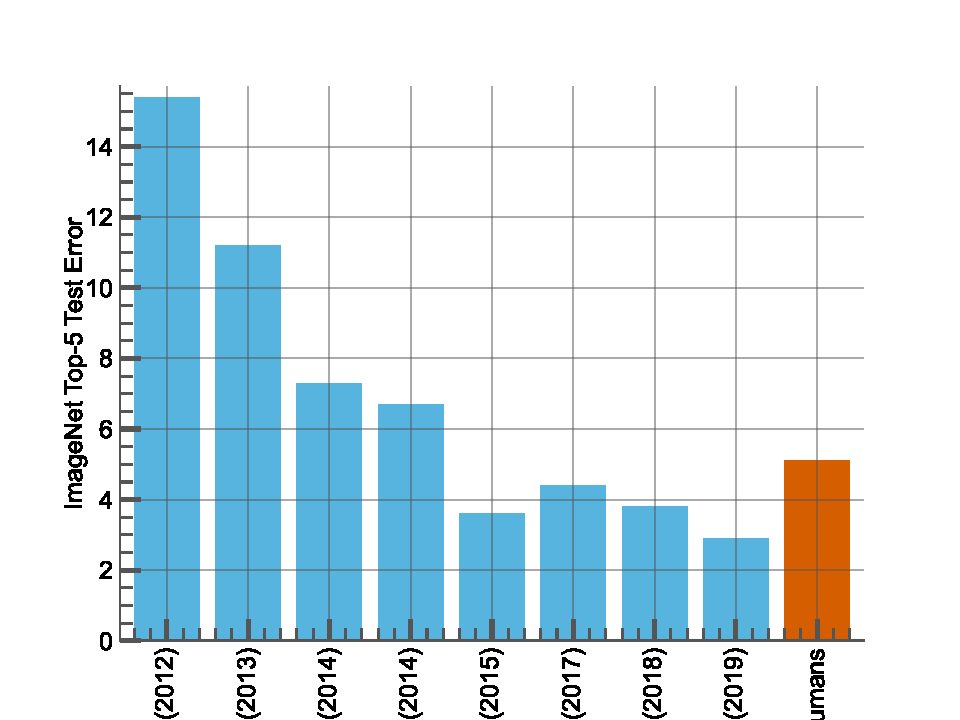
\includegraphics[width=0.8\textwidth]{chapter_intro/assets/models_vs_human.pdf}
      \caption{Models top-5 accuracy on ImageNet \cite{deng2009imagenet} compared
            to human performance.}
      \label{fig:intro:models_vs_humans}
\end{figure}

Given the nature of tasks the Netatmo cameras are designed to perform, deep
learning and \aclp{DNN} are not just a choice but a necessity. They represent
the state of the art in computer vision tasks that outperforms other algorithms
and allows for accurate and reliable object detection and recognition.\\

\section{Challenges}

While deep learning, particularly through the use of \acp{CNN}, is the
technology of choice for computer vision applications, it comes with its
challenges that need to be addressed, especially in the context of deploying
these deep and large models on embedded devices. These challenges include model
complexity and computational requirements. The necessity of compressing neural
networks has been highlighted previously and also comes with its challenges that
include: preserving the performance and controlling the size of the compressed
model as well as training time.\\

One of the most significant challenges in deploying deep learning models and
especially \acp{CNN} on embedded devices is the large model size. These models
often have millions of parameters and this makes them computationally heavy and
challenging to fit into the limited memory of embedded devices. Secondly, these
complex models require substantial computational resources to operate. This
translates into slow computations which is a critical issue for devices which
aim to perform real-time tasks.\\

Compressing large neural networks is a necessity to deploy them on embedded
devices. However, this compression process comes with its challenges. First, the
compressed model should maintain the performance of the original model. However,
the original large model is trained with all its parameters and thus depends on
all of them. Consequently, removing more than a few can lead to degraded
performance. \\

Second, the compressed model should be small enough to fit into the
limited memory of embedded devices. It means that the compression process should
be controlled to ensure that the size of the compressed model does not exceed
the memory budget. However, compressing the model too much can lead to an
irrecoverable loss in performance. The compression procedure and hyperparameters
should be carefully chosen to ensure that the compressed model has enough
capacity to perform the task at hand. This is often achieved by grid-searching
the optimal set of hyperparameters, which can be time-consuming.\\

Third, the compression process should be fast enough to be practical. Indeed,
the compression process is often performed after the training of the original
model and often requires fine-tuning the compressed one to compensate for the
loss of performance. This fine-tuning step can be computationally expensive and
time-consuming, effectively doubling the training time of the model in some
scenarios.\\

To conclude, while deep learning and \acp{CNN} represent an exciting advancement
in computer vision applications, several challenges need to be addressed for
efficient and effective deployment on embedded devices. Addressing these
challenges forms the crux of this research, with a particular focus on model
compression techniques to reduce the size and complexity of neural networks
without significant loss in performance.\\


\section{Contributions}

This thesis tackles the challenge of compressing \acp{DNN} through pruning, a
technique that aims to reduce the size of a neural network by removing redundant
or unnecessary parameters, subsequently detailed in \cref{chap:sota}. The
contributions detailed in this manuscript focus on methods to identify the
parameters to prune as well as minimise the impact of their removal on the final
performance. These contributions are as follows:\\

\noindent \textbf{Budget-aware pruning with weight reparametrisation.} The two
main challenges when pruning a neural network are first, determining which
weights should be removed and then, mitigating the loss of performance
introduced by weight removal. The first challenge is often referred to as
determining the saliency of the weights, which is a score that reflects the
importance of the weights in the network. The second challenge is often
sidestepped and the pruned network is simply fine-tuned to recover the lost
performance. To address both of these challenges, we propose the following main
contributions:

\begin{itemize}
      \item A numerically stable reparametrisation function, used in both our
            weight reparametrisation and our budget regularisation loss
            (subsequently detailed), that acts as a surrogate differentiable
            $\ell_0$ norm.

      \item A weight reparametrisation that embeds the saliency score of the
            weight in its expression and therefore value. This reparametrisation
            allows to soft-prune the weights during training thereby significantly
            mitigating the performance drop that occurs after pruning. Moreover,
            this reparametrisation does not require the introduction of auxiliary
            variables to determine the saliency of the weights, leading to a
            minimal impact on memory and computational requirements.

      \item A budget regularisation loss that allows to drive the optimisation
            procedure to respect a given budget. This budget regularisation loss
            benefits directly from the aforementioned reparametrisation function
            to compute the current weight budget. It is optimised jointly with
            the original loss, leading to an optimal solution in terms of
            performance and budget.

      \item A comprehensive set of experiments that demonstrate the
            effectiveness of our method and validate each one of its components
            on various datasets and architectures.\\
\end{itemize}

\noindent These contributions have been published in the following article:
\begin{itemize}
      \item Robin Dupont, Hichem Sahbi, and Guillaume Michel. Weight
            reparametrization for budget-aware network pruning. In \emph{2021
            IEEE International Conference on Image Processing, ICIP 2021,
            Anchorage, AK, USA, September 19-22, 2021}, pages 789–793. IEEE,
            2021.\\
\end{itemize}



\noindent \textbf{Pruning without weight training with stochastic sampling.} As
mentioned above, a major hurdle in pruning is determining which weights to
remove. This is especially challenging since weights, and consequently their
saliency, can fluctuate throughout training. This implies that pruning should
either be reversible or performed at the end of training. We propose a different
approach that does not require training the network to determine the saliency of
the weights, the latter being fixed throughout the process. Instead, we sample a
subset of weights (effectively pruning the other weights) forming a subnetwork
of the original network and evaluate its performance. This allows us to search
for a topology that is both lightweight and performant inside the original
network without training its weights. The main contributions of this method are
as follows: \\

\begin{itemize}
      \item A stochastic weight sampling method that is computationally
            efficient, numerically stable, differentiable and allows sampling
            weights while training their probability of being selected,
            represented by latent masks. The optimisation of the latter allows
            to learn the saliency of the weights without training the network,
            and therefore identifying and extracting an effective subnetwork.

      \item A pruning strategy for the masks that freeze the topology and
            performs better than averaging methods previously used in the
            state-of-the-art. Moreover, this pruning strategy allows to discover
            the optimal pruning rate for the network, eliminating the need for
            costly grid search to determine it.

      \item An efficient learnt-based weight rescaling mechanism to compensate
            for the disruption in weight distribution statistics caused by
            stochastic sampling. This rescaling is less computationally
            intensive, more flexible and allows for smoother variations of the
            scaling factor than other rescaling methods.

      \item A comprehensive set of experiments that demonstrate the
            effectiveness of our method and validates each one of its components
            on various datasets and architectures, as well as comparison with
            other closely related state-of-the-art methods in various
            configurations.

      \item A public repository containing the implementation of our method and
            the methods we compare against, as well as detailed code and instructions to
            reproduce our results.\\
\end{itemize}

\noindent These contributions have been published in the following article:
\begin{itemize}
      \item Robin Dupont, Mohammed Amine Alaoui, Hichem Sahbi, and Alice
            Lebois. Extracting effective subnetworks with Gumbel-Softmax. In \textit{2022
                  IEEE International Conference on Image Processing, ICIP 2022, Bordeaux,
                  France, 16-19 October 2022,} pages 931–935. IEEE, 2022.\\
\end{itemize}

\section{Outline}

The rest of this thesis is organised as follows:\\

\Cref{chap:dlo} offers an introduction to deep learning, providing a detailed
overview of its foundational and core concepts. It first explores early
architectures, beginning with the \emph{Perceptron} and the \ac{MLP}. The focus
of the chapter then shifts towards neural network training, giving formal
definitions of the loss function, regularisation, and optimisation process. A
dedicated section delves into \aclp{CNN}, exposing and detailing their building
blocks, and the evolution of their architectures. Then, the architectures used
in the experiments of \cref{chap:chapter1,chap:chapter2} are detailed.
Additionally, this chapter lists and describes prominent datasets, namely
CIFAR-10, CIFAR-100, and TinyImageNet, and discusses their respective train,
validation, and test sets.\\

\Cref{chap:sota} introduces deep neural network compression and presents
state-of-the-art methods divided into different families. The chapter begins
with acceleration techniques and presents a range of methods whose goal is to
speed up matrix operations or convolutions. Then, it explores the teaching
paradigm, highlighting methods that rely on a large pre-trained network to
improve the training of lightweight ones. Furthermore, the chapter addresses the
design aspects of lightweight architectures introducing building blocks for
efficient architecture design and \acl{NAS}. Afterwards, the chapter discusses
methods to compress and optimise existing architectures and in particular
pruning. Finally, the chapter presents the positioning of our methods and the
rationale behind them.\\

\Cref{chap:chapter1} presents our pruning method based on weight
reparametrisation and budget regularisation. It starts by outlining closely
related work. Then, the core method components are examined, starting with our
weight reparametrisation and then our budget loss. Afterwards, a general
overview of the algorithm is provided. Furthermore, the chapter details
experiments assessing our method performance in various configurations as well
as experiments validating the components of our method and the choices of
hyperparameters. A conclusion summarises the key findings and highlights of our
method for neural network pruning.\\

\Cref{chap:chapter2} delves into our stochastic pruning method without weight
training. It starts with an introduction and examination of closely related
work. Then, it details the first core component of our method, namely
\acl{ASLP}, a method for extracting effective subnetworks using the
Gumbel-Softmax technique that solves various issues that arose from previous
methods. Afterwards, it introduces our weight-rescaling technique and presents
its main benefits, as well as our pruning strategy to freeze the stochastic
topology. Subsequently, a method and algorithm overview outlines the key points
of our methods. Furthermore, the chapter exposes a comprehensive set of
experiments that compares our method against other state-of-the-art methods in
various scenarios and validates the components of our method. The chapter
concludes by summarising our findings and results.\\
\chapter{Deep Learning Overview}\label{chap:dlo}

\localtableofcontents

\section{Introduction}

Deep learning is a subfield of machine learning that focuses on the study of
\acp{DNN}. Deep Learning is a family of machine learning algorithms called
\acp{DNN} that have their roots in \acp{ANN} which aim to learn a data
representation from unstructured data such as raw images
\cite{DBLP:conf/nips/KrizhevskySH12}, text
\cite{DBLP:conf/emnlp/BudzianowskiV19} or audio
\cite{DBLP:journals/corr/HannunCCCDEPSSCN14}, in an end-to-end fashion.
\acp{ANN} were initially conceptualised based on the understanding of biological
neural networks present in the brain
\cite{mcculloch1943logical,hebb2005organization}.
\citeauthor{rosenblatt1958perceptron} proposed in
\cite{rosenblatt1958perceptron} a theoretical model of a neuron, denoted the
\emph{perceptron}, which was capable of learning a linear decision boundary. The
perceptron model was later extended to multiple layers of neurons, giving rise
to the \ac{MLP} \cite{rosenblatt1961principles,rumelhart1986learning}. A
\acl{MLP} is a type of artificial neural network that extends the concept of a
single-layer perceptron by including one or more hidden layers of neurons
connected upstream to an input layer and downstream to an output layer. Each
layer is fully connected to the next, allowing the model to learn and represent
more complex, non-linear relationships in the input data. Although able to learn
more complex boundaries than the perceptron, the \ac{MLP} is still limited by
its depth. The next advance came from the stacking of multiple layers, leading
to \aclp{DNN}.\\

In the context of \acp{DNN}, the term \emph{deep} denotes the stacking of many
layers within a neural network. The concept of \acp{DNN} is based on the idea
that the depth and the numerous layers can help in learning features at various
levels of abstraction, enabling the network to learn complex hierarchical
patterns. For instance, in the context of image recognition, lower layers may
learn local features like edges and textures, while deeper layers might learn to
identify more abstract concepts like shapes or objects.\\

The rise of \acp{DNN} was made possible by several factors. On the one hand the
increase in computational power, and in particular the use of \acp{GPU}, which
made the training of deep networks feasible. Indeed, AlexNet, the first \ac{CNN}
to win the ImageNet Large Scale Visual Recognition Challenge
\cite{DBLP:conf/nips/KrizhevskySH12}, was trained on two \acp{GPU} in parallel
to accelerate computations. Nowadays, the use of \acp{GPU} or dedicated hardware
such as \acp{TPU} is ubiquitous and supported by all the major deep learning
frameworks
\cite{DBLP:journals/corr/AbadiABBCCCDDDG16,DBLP:conf/nips/PaszkeGMLBCKLGA19}.On
the other hand, the availability of large-scale datasets such as ImageNet
\cite{deng2009imagenet} allowed to train or pre-train deep networks with
millions of parameters without overfitting.\\

This chapter aims to give an overview of the different neural network
architectures, building blocks, training techniques and datasets that are widely
used in Deep Learning for computer vision as well as our experiments.
\Cref{sec:dlo:early_architectures} introduced the early neural network
architectures, namely the perceptron and the \ac{MLP}. \Cref{sec:dlo:training}
focuses on the functional definition of a neural network and its training.
\Cref{sec:dlo:cnn} presents the building blocks and architectures of various
\acp{CNN} for computer vision, and in particular the ones we benchmark our
methods with (see \cref{sec:chap1:experiments,sec:chap2:experiments}). Finally,
\Cref{sec:dlo:datasets} gives an overview of the most used datasets that we
used in our experiments.


\section{Early Architectures}\label{sec:dlo:early_architectures}

In this section, we present the perceptron \cite{rosenblatt1958perceptron} and
then the \acl{MLP} \cite{rosenblatt1961principles,rumelhart1986learning}. Both
are the two founding neural network architectures that led to the development of
\aclp{DNN}.

\subsection{Perceptron}\label{sec:dlo:perceptron}

The \emph{perceptron} is a model of artificial neuron, capable of learning a
linear decision boundary. It was proposed by
\citeauthor{rosenblatt1958perceptron} in 1958 \cite{rosenblatt1958perceptron}
and conceptualised based on the understanding of biological neural networks
present in the brain \cite{mcculloch1943logical,hebb2005organization}. The
perceptron is composed of inputs that are weighted and summed before being
passed through a nonlinear function referred to as an activation function. The
conceptrual representation of the perceptrion is displayed in
\cref{fig:dlo:perceptron} and its mathematical formulation is defined in
\cref{eqn:dlo:perceptron}: \\
% and can be express in vector form as written in \cref{eqn:dlo:perceptron_vector}.\\

\begin{equation}
  \label{eqn:dlo:perceptron}
\hat{y} = g(\sum_{i=1}^{n} w_i \cdot x_i + b)
\end{equation} \\


% \begin{equation}
%   \label{eqn:dlo:perceptron_vector}
%   \hat{y} = g(\mathbf{w}^T \mathbf{x} + b)
% \end{equation}\\

\noindent where $x_i$ is the $i$th input, $w_i$ is the weight associated with
the $i$th input,$n$ is the number of inputs, $b$ is the bias, $g$ is the
activation function, and $\hat{y}$ is the perceptron's output. This formulation
can also be written in vector form as in \cref{eqn:dlo:perceptron_vector}: \\

\begin{equation}
  \label{eqn:dlo:perceptron_vector}
  \hat{y} = g(\mathbf{w}^T \mathbf{x} + b)
\end{equation}\\

\noindent where $\mathbf{x}$ is the vector of inputs and $\mathbf{w}$ is the
vector of weights. The activation function is typically a nonlinear function,
such as the sigmoid function or the hyperbolic tangent function. Due to its
shallow architecture, the perceptron cannot learn complex decision boundaries.
Nevertheless, it is possible to stack several perceptrons to learn nonlinear
decision boundaries, leading to a \acl{MLP}.\\

\begin{figure}[htbp]
  \centering
  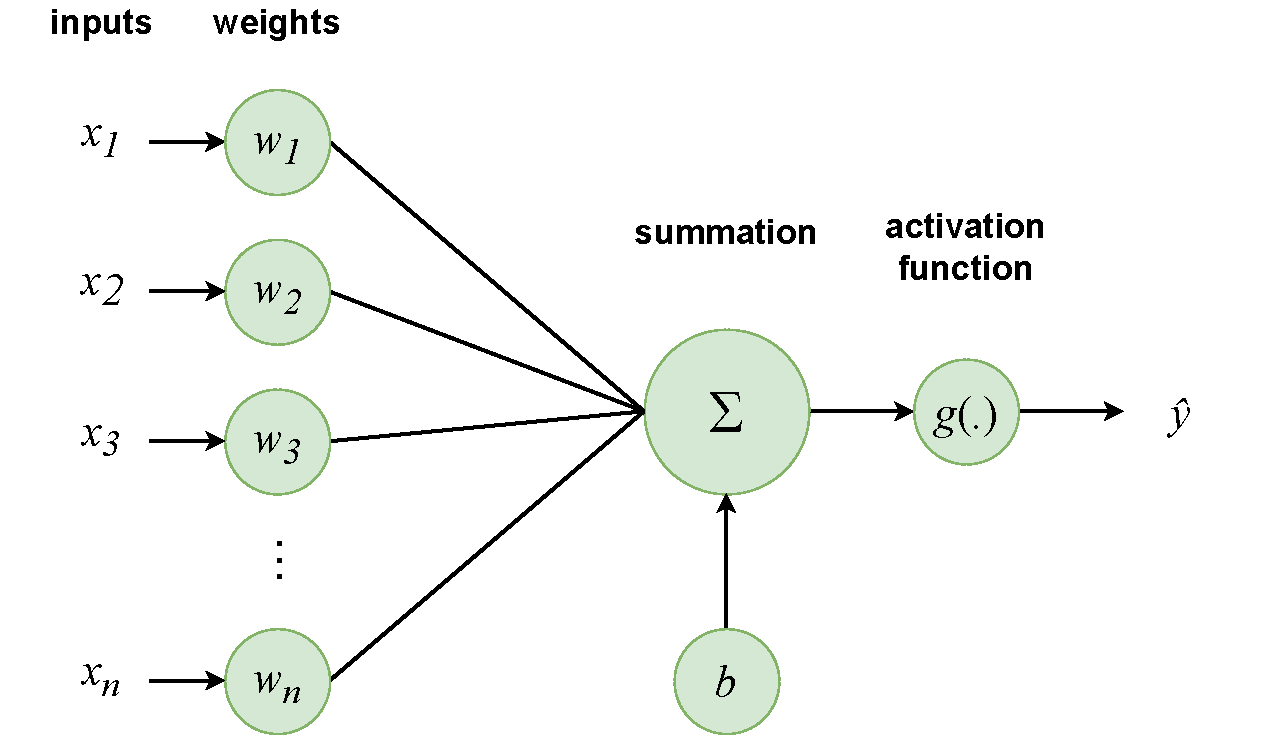
\includegraphics[width=0.7\textwidth]{chapter_dlo/assets/perceptron_scheme.pdf}
  \caption{Conceptual scheme of the \emph{perceptron}. Each input $x_i$ is multiplied
  by its associated weight $w_i$ and summed to the other weighted inputs. The
  bias $b$ is added to the sum and the result is passed through an activation
  function $g$ to produce the output $\hat{y}$.}
  \label{fig:dlo:perceptron}
\end{figure}

\subsection{Multilayer Perceptron}\label{sec:dlo:mlp}


The \acf{MLP} is an extension of the perceptron model, comprising multiple
layers of perceptrons, also referred to as neurons \cite{rumelhart1986learning}.
A \ac{MLP} with one hidden layer is represented in \cref{fig:dlo:mlp}. In the
latter, the circles represent the neurons, and the connections between
representing weights are materialised by lines. The \ac{MLP} is the simplest
type of feedforward \ac{ANN}. Feedforward refers to the fact that the
connections between neurons in the \ac{MLP} form a \acf{DAG}, where the outputs
of the neurons from one layer are passed to the next, with no backward
connections or feedback. Using the same notations as in
\cref{eqn:dlo:perceptron_vector}, the vector form of the \ac{MLP} displayed in
\cref{fig:dlo:mlp} can be written as in \cref{eqn:dlo:mlp}, where the subscript
of activation functions $g_i$, weight matrices $\mathbf{w}_i$ and bias vectors
$\mathbf{b}_i$ denotes their belonging to the $i$th layer.\\

\begin{equation}
  \label{eqn:dlo:mlp}
  \hat{\mathbf{y}} = g_2(\mathbf{w}_2^T \cdot  g_1(\mathbf{w}_2^T \cdot \mathbf{x} + \mathbf{b}_1) + \mathbf{b}_2)
\end{equation}\\

Each layer of the \ac{MLP} being fully connected to the next one, it enables the
\ac{MLP} to handle problems that the perceptron cannot solve, such as problems
requiring nonlinear decision boundaries. Furthermore,
\citeauthor{cybenko1989approximation} proved in \cite{cybenko1989approximation}
that an \ac{MLP} can approximate continuous functions on compact subsets of
$\mathbb{R}^n$. This result is known as the \emph{Universal Approximation
Theorem}. Before the emergence of Deep Learning, \acp{MLP} have been applied to
various domains, including voice recognition, image recognition, and machine
translation \cite{wasserman1988neural}.


\begin{figure}[htbp]
  \centering
  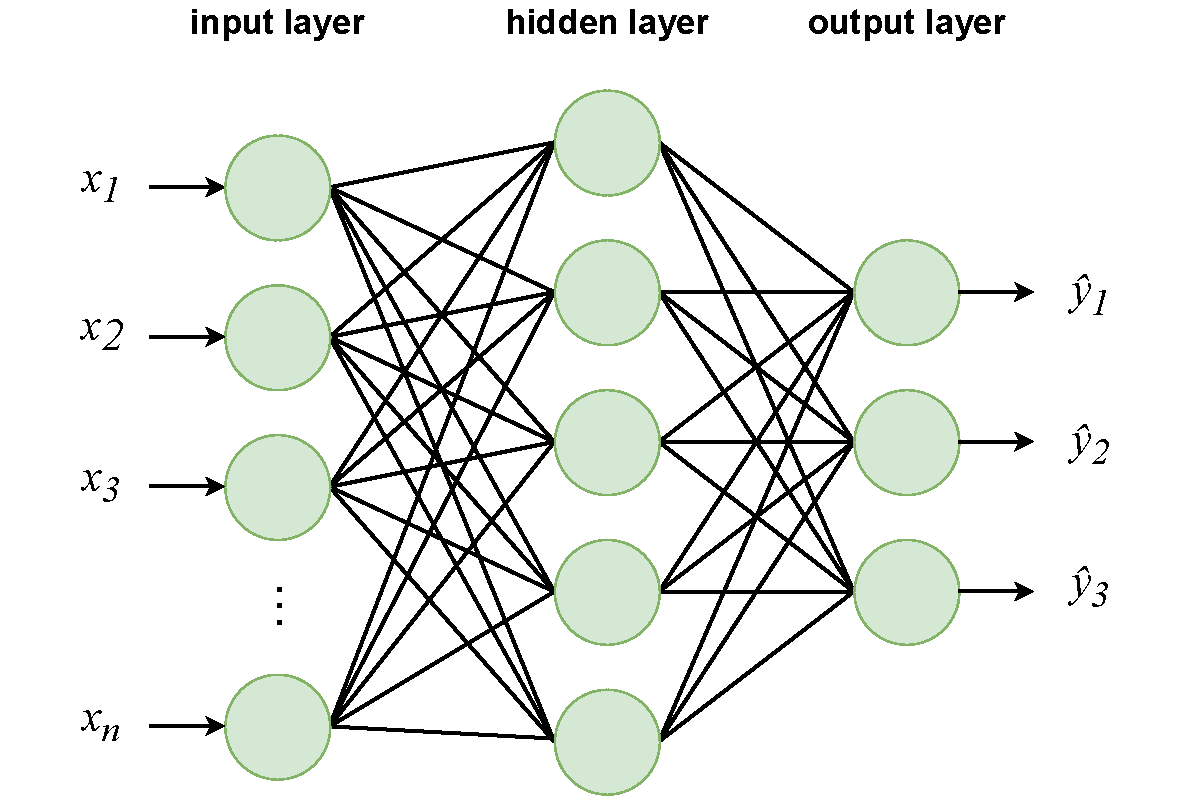
\includegraphics[width=0.7\textwidth]{chapter_dlo/assets/mlp_scheme.pdf}
  \caption{Conceptual scheme of a \ac{MLP} with one hidden layer. Each circle
  represent a neuron and each line a connection associated with a weight.}
  \label{fig:dlo:mlp}
\end{figure}

\section{Neural Network Training}\label{sec:dlo:training}

Neural Network Training revolves around the optimisation of a mapping function
that learns to predict an output given input data by adjusting its internal
parameters, also referred to as weights. This optimisation, also called
\emph{training}, involves iteratively tuning these weights so that the
discrepancy between the output predicted by the model and the reference output
is minimised. Weights tuning relies on gradient-based methods that hinge
arround to core components: the \emph{backpropagation} algorithm to compute the
gradients and the \ac{SGD} algorithm to update the weights.

\subsection{Functional Definition}

Neural networks can be defined as a mapping function from an input space
$\mathcal{X}$ to an ouput space $\mathcal{Y}$. This mapping function $f$ is
parametrised by a set of parameters $\theta$, often called \emph{weights}. The
training of a neural network consists in tuning the parameters $\theta$ so that,
given an input $X_i$, the mapping function $f$ output, denoted $\hat{y}_i$, is
as close as possible to the associated true output $y_i$. This training is done
iteratively by using example pairs $(X, y) \in \mathcal{X} \times \mathcal{Y}$,
where $X\in\mathcal{X}$ is the input and $y\in\mathcal{Y}$ is the output. In the
context of image classification, $X$ is an image and $y$ is a label that
indicates the class of the associated image. A functional representation of a
neural network is given in \cref{eqn:dlo:nn_functional_definition}, where $f$ is
the neural network, $\theta$ is the set of parameters of the network,
$X\in\mathcal{X}$ is the input given to the neural network and $\hat{y}$ is the
output.\\

\begin{equation}
  \label{eqn:dlo:nn_functional_definition}
  % \centering
  \begingroup
  \setlength\arraycolsep{0pt}
  f \colon\begin{array}[t]{c >{{}}c<{{}} l}
    \mathcal{X} & \to     & \mathcal{Y} \\
    X                     & \mapsto & f(X, \theta) = \hat{y}
  \end{array}
  \endgroup
\end{equation}\\


Considering image classification,  the output $\hat{y}$ is a probability vector
where the largest coefficient is the one whose index corresponds to the
predicted class of the input image, often called a label. This vector is
generally converted into a one-hot vector, where the only non-zero coefficient is
at the index of the predicted class. The true label $y$, referred to as the
ground truth is either the class index and $y\in\llbracket0;n-1\rrbracket$,
where $n$ is the number of classes considered. The ground truth can also be
converted into a one-hot vector.\\

% In the case of image classification, the input $X$ given to the neural network
% is an image, and the output $\hat{y}$ is a probability vector where the largest
% coefficient is the one whose index corresponds to the predicted class of the
% input image. $y_i$, often referred to as the ground truth is a one-hot vector
% where the only non-zero coefficient is at the index corresponding to the true
% class of the input image.\\

% A neural network is a function that maps an input $X$ to an output $y$ through
% a series of transformations. The functional definition of a neural network is
% given in \cref{eqn:dlo:nn_functional_definition}, where $f$ is the neural
% network, $\theta$ is the set of parameters of the network, and $y$ is the
% output.\\

\subsection{Loss Function and Regularisation}
Training a neural network aims at finding the optimal parameters $\theta$ that
maximises a performance, quantified by the metric $P$, often based on the
discrepancy between the predicted output $\hat{y}$ and the true output $y$.
However, optimising directly the metric $P$ might be intractable. To solve for
this issue, we define a differentiable cost function and minimise the latter as
a proxy for optimising $P$. Considering $\delta$ as the empirical distribution
of the training data, the cost function $\mathcal{J}(\theta)$, also denoted the
\emph{empirical risk} is defined as:

\begin{equation}
  \label{eqn:dlo:cost_function}
  \mathcal{J}(\theta) = \mathds{E}_{(X, y) \sim \delta} \left[ \mathcal{L}(f(X,\theta), y) \right]
\end{equation}\\

\noindent where $\mathcal{L}$ is the loss function. Note that the true data
distribution is not known, and thus, the empirical distribution $\delta$ is used
instead. The minimisation of the empirical risk alone is not sufficient. Indeed,
the neural network could learn to perfectly predict the output of the training
set but fail to generalise to unseen data. This phenomenon is called
\emph{overfitting}. To prevent overfitting, we add a regularisation term to the
empirical risk. The regularisation term, denoted $\mathcal{R}$, is a function of
the parameters $\theta$ of the neural network which penalises the complexity of
the model, and thus prevents overfitting. To account for regularisation, the
cost function in \cref{eqn:dlo:cost_function} is updated to:

\begin{equation}
  \label{eqn:dlo:regularised_cost_fn}
  \mathcal{J}_r(\theta) = \mathds{E}_{(X, y) \sim \delta} \left[ \mathcal{L}(f(X,\theta), y) + \mathcal{R}(\theta) \right]
\end{equation}\\

\noindent\textbf{Loss function.} In
\cref{eqn:dlo:cost_function,eqn:dlo:regularised_cost_fn}, the loss function
$\mathcal{L}$ is a measure of the discrepancy between the ground truth $y$ and
the predicted output. Contrary to the metric $P$ which might be
non-differentiable, the loss function is differentiable so that its minimisation
can be achieved using gradient-based methods, subsequently detailed in
\cref{sec:dlo:backpropagation}. The choice of the loss function depends on the
task at hand. For classification tasks (not only images), the loss function is
often the \emph{cross-entropy} loss. For a binary classification problem, the
ground truth is a binary variable $y\in \{0,1\}$ and the predicted output is a
scalar $f(X,\theta)=\hat{y}\in[0,1]$. The binary cross-entropy loss is defined
as follows:\\

\begin{equation}
  \label{eqn:dlo:binary_cross_entropy_loss}
  \mathcal{L}(\hat{y}, y) = - y \log(\hat{y}) - (1-y) \log(1-\hat{y})
\end{equation}\\

\noindent The binary cross-entropy loss defined in
\cref{eqn:dlo:binary_cross_entropy_loss} can be extended to problems with more
than two classes. For a classification problem with $c$ classes, the ground
truth is a one-hot vector $\mathbf{y}\in \{0,1\}^c$ and the output is a
$c$-dimensional vector $f(X,\theta)=\hat{\mathbf{y}}\in\mathds{R}^c$. The
multi-class cross-entropy loss is defined as follows:

\begin{equation}
  \label{eqn:dlo:multiclass_cross_entropy_loss}
  \mathcal{L}(\hat{\mathbf{y}}, \mathbf{y}) = - \sum_{i=1}^c y_i \log \left( \displaystyle\frac{\exp(\hat{y}_i)}{\displaystyle\sum_{j=1}^c \exp(\hat{y}_j)} \right)
\end{equation}\\

\noindent In the above equation, $\hat{\mathbf{y}}$ is the unormalised raw
output vector of the neural network and $\phi$ is the softmax function, whose
expression is given in \cref{eqn:dlo:softmax}. The softmax function is used to
convert the raw output vector of real numbers into a probability distribution.
Note that some models output directly a probability distribution, in which case
the softmax is not needed.\\

\begin{equation}
  \label{eqn:dlo:softmax}
  \phi(\mathbf{z})_j = \frac{\exp(z_j)}{\displaystyle\sum_{k=1}^{\text{dim}(\mathbf{z})} \exp(z_k)}
\end{equation}\\

\noindent \textbf{Regularisation.} The regularisation term $\mathcal{R}$ is a
differentiable function of the weights $\theta$. It acts as a control mechanism
to avoid overfitting by preventing the weights of the neural network from
becoming too large, which can lead to overly complex models that overfit the
training data. This is typically achieved by adding a penalty proportional to
the magnitude of the weights, thereby keeping them small.\\

Common types of regularisation include $\ell_1$ and $\ell_2$ regularisation,
whose expressions are shown in \cref{eqn:dlo:reg_l1,eqn:dlo:reg_l2}
respectively. $\ell_1$ regularisation \cite{tibshirani1996regression}, adds a
penalty equal to the absolute value of the magnitude of the weights. On the
other hand, $\ell_2$ regularisation \cite{hoerl1970ridge}, adds a penalty
equivalent to the square of the magnitude of the weights. Both methods aim to
reduce the magnitude of the weights, but $\ell_1$ regularisation is more
targeted towards feature selection, effectively pushing some weights to $0$,
whereas $\ell_2$ restrains globally their magnitude.\\

The regularisation term $\mathcal{R}$ is added to the cost function with a
regularisation coefficient, usually denoted as $\lambda$, which is a
hyperparameter that balances the trade-off between fitting the training data
(minimising the loss $\mathcal{L}$) and limiting the complexity of the model
(minimising $\mathcal{R}$).

\begin{equation}
  \label{eqn:dlo:reg_l1}
  \mathcal{R}_{\ell_1}(\theta) = \lambda \sum_{i=1}^{\text{dim}(\theta)} \left| \theta_i \right|
\end{equation}\\

\begin{equation}
  \label{eqn:dlo:reg_l2}
  \mathcal{R}_{\ell_2}(\theta) = \frac{\lambda \| \theta \|_2}{2} 
\end{equation}\\

\subsection{Loss Optimisation}\label{sec:dlo:backpropagation}

As mentioned before, the training of a neural network involves finding the
optimal set of parameters $\theta$ that minimises a cost function
$\mathcal{J}(\theta)$. This process of optimisation is typically carried out
using gradient-based methods which rely on the iterative adjustment of the
parameters in the opposite direction of the gradient of the cost function. The
gradient of a function provides the direction of the steepest ascent at a given
point \cite{boyd2004convex}. Thus, by moving the parameters in the opposite
direction of the gradient, we seek to descend to a local minimum of the
function.\\

\noindent \textbf{Backpropagation.} One critical step in the optimisation
process is the computation of the gradient of the cost function with respect to
the parameters, $\nabla \mathcal{J}(\theta)$. These gradients are computed with
the \emph{backpropagation} algorithm \cite{rumelhart1986learning} which is an
application of the \emph{chain rule} (see \cref{eqn:dlo:chain_rule}) to
efficiently compute these gradients. It involves a forward pass through the
network to compute the outputs and thus the loss, and a backward pass to
calculate the gradients. During the backward pass, the partial derivative of the
cost with respect to each parameter is computed, starting from the output layer
and going back to the input layer. The previously computed derivatives from the
subsequent layers are used to compute the ones of the earlier layers,  
making the backpropagation algorithm computationally efficient.\\

% Chain rule latex equation
\begin{equation}
  \label{eqn:dlo:chain_rule}
  \frac{\partial z}{\partial x} = \frac{\partial z}{\partial y} \frac{\partial y}{\partial x}
\end{equation}\\

\noindent \textbf{\acl{SGD}.} Once the gradients are calculated, they are
used to update the parameters. The most prevalent for parameter updates is
\acf{SGD}, a derivative of the Robbins–Monro algorithm
\cite{robbins1951stochastic}. In \ac{SGD}, the gradient of the loss function is
computed for a random subset of the data (a \emph{batch} or \emph{mini-batch}),
and the weights are shifted in the direction that decreases the loss function.
This is achieved by subtracting the gradient of the cost function with respect
to that parameter multiplied by a learning rate $\eta$:\\

\begin{equation}
\label{eqn:dlo:sgd_update}
\theta_i^{(t+1)} = \theta_i^{(t)} - \eta \frac{\partial \mathcal{J}(\theta)}{\partial \theta_i}
\end{equation}\\

\noindent where $\theta_i^{(t)}$ is the $i$th parameter at iteration $t$. The
\ac{SGD} algorithm is detailed in \cref{alg:dlo:sgd}. The use of mini-batches in
\ac{SGD} leads to a trade-off between computational efficiency and estimation
accuracy. Indeed, the gradient is estimated using a subset of the entire
training set, which is, on the one hand, less accurate than using the whole
dataset, but on the other hand, less computationally intensive. The size of the
minibatch, which is a hyperparameter of the training algorithm, determines this
trade-off and should also be chosen depending on the computational and memory
resources available. Note that the size of modern datasets, subsequently
detailed in \cref{sec:dlo:datasets}, makes it intractable to evaluate the
gradients on the whole dataset in one step.\\

\begin{algorithm}
  \caption{Stochastic Gradient Descent Algorithm}
  \label{alg:dlo:sgd}
  \begin{algorithmic}
    \REQUIRE {Learning rate $\eta$, minibatch size $m$,Initial parameters
    $\theta^{(0)}$, $n>m$ training pairs $(X,y)\in
    \mathcal{X}\times\mathcal{Y}$, Loss function $\mathcal{J}$}
    \WHILE {Stopping criterion not met}
    \STATE {Sample minibatch of size $m$ from training set}
    \STATE {Compute gradient estimate on minibatch: $\hat{g} \gets \nabla \mathcal{J}(\theta)$}
    \STATE {Update parameters: $\theta^{(t+1)} \gets \theta^{(t)} - \eta \hat{g}$}
    \ENDWHILE
    \RETURN {Optimal parameters $\theta$}
  \end{algorithmic}
\end{algorithm}


\noindent \textbf{Learning Rate.} The learning rate is a hyperparameter that
determines the step size of the update at each iteration while moving toward a
minimum of the loss function. Setting the learning rate too high can cause the
learning process to converge too quickly or overshoot while setting it too low
can make the learning process slow to converge, as shown in
\cref{fig:dlo:gradient_descent}.\\

\begin{figure}[htbp]
  \centering
  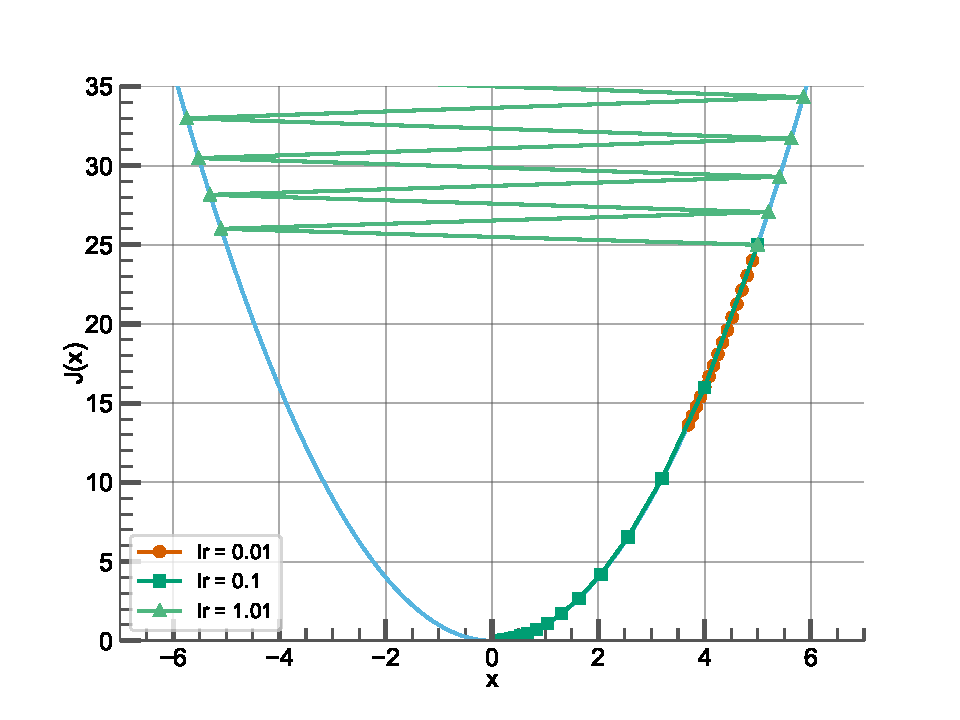
\includegraphics[width=0.7\textwidth]{chapter_dlo/assets/gradient_descent.pdf}
  \caption{Illustration of the effect of the learning rate on the convergence of
    the gradient descent. The gradient descent has been applied iteratively for
    20 epochs. On the one hand, a too-high learning (1.01) rate causes the
    gradient descent to overshoot the minimum of the loss function. On the other
    hand, a too-low learning rate (0.01) causes the gradient descent to converge
    slowly.}
  \label{fig:dlo:gradient_descent}
\end{figure}

\noindent \textbf{Alternative methods.} To enhance the performance of \ac{SGD},
various modifications and extensions have been proposed, such as \ac{SGD} with
momentum \cite{sutskever2013importance}, RMSProp \cite{hinton2012neural}, or
Adam \cite{kingma2014adam}. These methods aim to adjust the learning rate
dynamically or dampen the oscillations in the gradient descent to achieve faster
and more stable convergence.\\

For instance, \ac{SGD} with momentum \cite{sutskever2013importance} uses a
momentum term $\gamma$ to dampen the oscillations in the gradient descent. It
allows smoothing the variations of the descent direction and thus, preventing
the optimisation to get stuck in small local minimums. The momentum term is a
moving average of the gradients, here denoted $v$, and it is used to update the
parameters as shown in \cref{eqn:dlo:sgd_momentum_update}. In this equation, the
momentum term $\gamma \in [0,1]$ is a hyperparameter that is typically set close
to 1, $0.9$ being a common value.\\

\begin{equation}
  \label{eqn:dlo:sgd_momentum_update}
  \begin{split}
    v_{t+1} &= \gamma v_t + \eta \nabla \mathcal{J}(\theta) \\
    \theta_{t+1} &= \theta_t - v_{t+1}
  \end{split}
\end{equation}\\

\section{Convolutional Neural Networks for Computer Vision}\label{sec:dlo:cnn}

In the field of computer vision, \acp{CNN} have emerged as effective
architectures that enable high performance on image classification tasks. The
effectiveness of \acp{CNN} lies in their architecture that leverages the \ac{CL}
layers to automatically learn abstract features from visual data in a
hierarchical fashion. In this section, we explore the building blocks of
\acp{CNN} and various architectures that have been widely used and became
\emph{de facto} standards in the literature.

\subsection{Building Blocks}

This section covers the most common building blocks of \acp{CNN} for computer
vision. These building blocks are organised in layers that are stacked to form
neural network architectures subsequently detailed in
\cref{sec:dlo:architectures}.\\

\noindent\textbf{Convolutional layer.} \ac{CL} layers are one of the core
building blocks of \acp{CNN}. Each convolution layer performs a series of
spatial convolutions on the input data using a set of learnable filters or
kernels. These filters are designed to extract low-level features such as edges,
corners, and textures in the early layers, while they learn high-level features
like object parts or even whole objects in the deeper layers. Contrary to manual
feature engineering, the features learned by \ac{CL} layers are learned in a
\emph{end-to-end} fashion. The convolution operation is defined in
\cref{eqn:dlo:convolution} :\\

\begin{equation}
  \label{eqn:dlo:convolution}
  (x * k)(i,j) = \sum_{m} \sum_{n} x(i -m, j -n) \cdot k(m, n)
\end{equation}\\

\noindent where, $x$ is the input, $k$ is the kernel, $(i,j)$ are the spatial
coordinates in the output feature map and $m$ and $n$ represents the spatial
coordinates of the kernel $k$. Note that some Deep Learning frameworks
implement \emph{cross-correlation} instead of convolution. In the former, the
kernel is not spatially flipped leading to the cross-correlation not being
commutative \cite{goodfellow2016deep}. The \ac{CL} layer kernels are typically
smaller than the input along width and height dimensions (they are generally
$3\times 3$ \cite{DBLP:conf/cvpr/HeZRS16}) but comprises as much channels as the
input. During the forward pass, each kernel is spatially convolved channel-wise
with the input and their outputs are summed along the channel dimension to yield
a single scalar for each kernel position on the input (see
\cref{fig:dlo:conv_layer}).\\

\ac{CL} are more computationally efficient than \ac{FC} layers, as they have a
form of weight sharing baked in. Indeed, the same kernel is applied to every
location of the input, which brings two main benefits: \emph{(i)} the number of
parameters is independent of the input size and \emph{(ii)} a single learned
kernel, acting as a feature detector, can be used in multiple locations. This is
especially useful for early feature detector that detects basic shapes or
textures. In addition, because of the kernels being convolved across the whole
input, \ac{CL} layers are also less sensitive to spatial translations that might
occur in different instances of the same class.

\noindent \textbf{Fully connected layer.} \ac{FC} layers, also known as
\emph{Dense} layers are often the last layers of a \ac{CNN}, effectively serving
as a classifier, whereas the \ac{CL} layers act as a feature extractor.
\ac{FC} layers perform high-level reasoning by conducting non-linear
transformations of the extracted features and combining them to make decisions.
In an FC layer, each neuron is connected to every neuron in the previous layer.
A \ac{FC} layer can be describe as a matrix-vector product as in
\cref{eqn:dlo:fc_layer} (see \cref{fig:dlo:dense_layer}).\\

\begin{equation}
  \label{eqn:dlo:fc_layer}
  y = \mathbf{w}^T \cdot \mathbf{x} + b
\end{equation}\\

\noindent where $\mathbf{x}$ is the input vector, $\mathbf{w}$ is the weight
matrix and $b$ is the bias. In the context of \acp{CNN}, before passing the
output of the last \ac{CL} layer to the first \ac{FC} layer, it needs to be
flattened or reshaped into a single column vector. The final layer in a \ac{CNN}
is a \ac{FC} layer that has a number of neurons equal to the number of output
classes, and it typically uses a softmax activation to output a probability
distribution over those classes.\\

%FIXME: rajouter phrase pour dire que l'on peut remplacer les layers FC par des
%layers conv pour des réseaux "fully convolutional"


\begin{figure}[htbp]
  \centering
  \subfloat[Convolutional Layer\label{fig:dlo:conv_layer}]{
    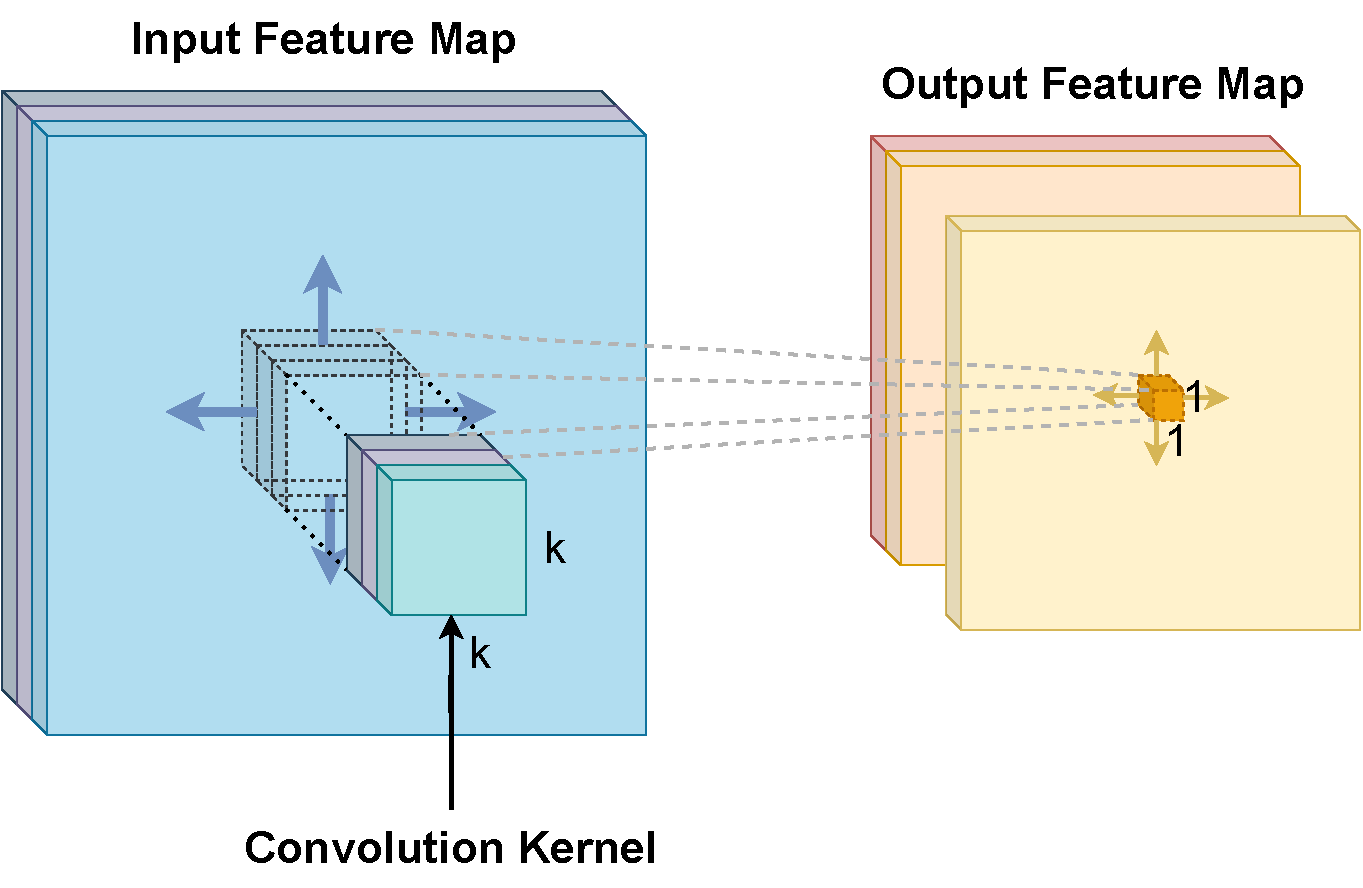
\includegraphics[width=0.49\textwidth]{chapter_dlo/assets/conv_layer.pdf}}
  \subfloat[Dense Layer\label{fig:dlo:dense_layer}]{
    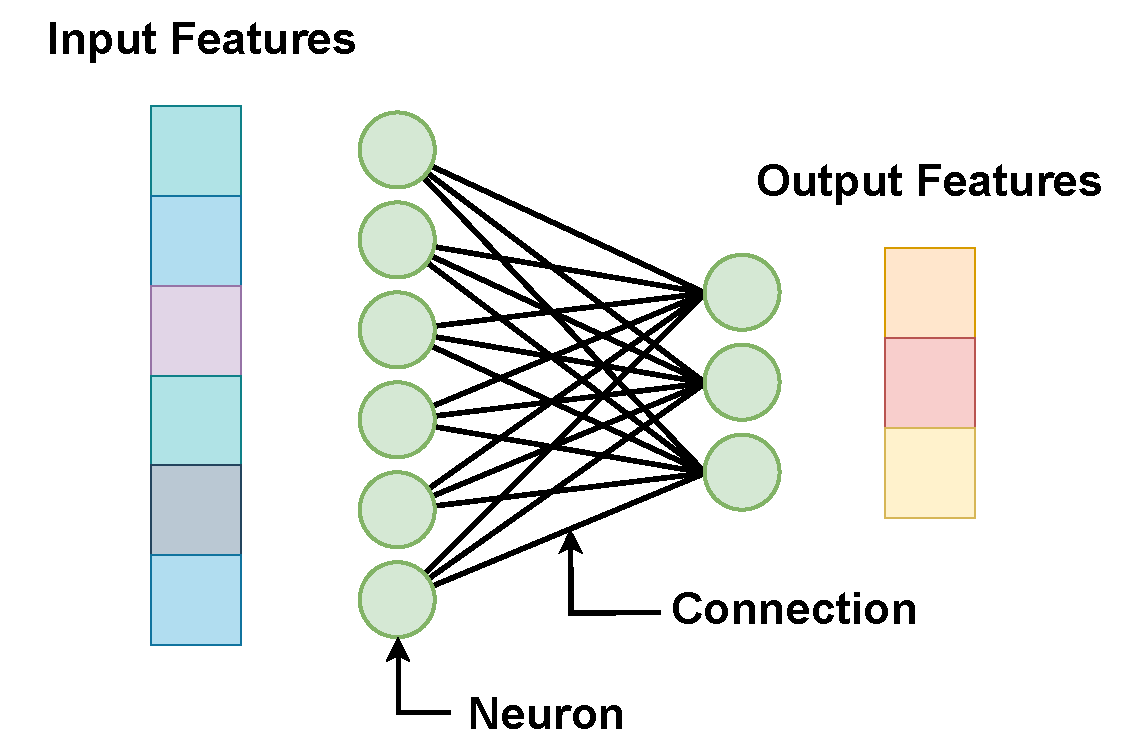
\includegraphics[width=0.49\textwidth]{chapter_dlo/assets/dense_layer.pdf}}
  \caption{Conceptual representation of a \acl{CL} and a dense
    layer. The \acl{CL} (\cref{fig:dlo:conv_layer}) takes a
    multi-channel input and produces a multi-channel output. Each coefficient of
    the output is computed by applying a convolution operation at a
    corresponding location in the input. The dense layer
    (\cref{fig:dlo:dense_layer}) takes a vector input and produces a vector
    output. Each connection is represented by a weight in the weight matrix.}
  \label{fig:sota:layers}
\end{figure}

\noindent \textbf{Activation function.} Activation functions are often applied to
the output feature map of a convolutional or fully connected layer. This
function introduces non-linearity into the model, allowing it to learn more
complex patterns \cite{long2015fully}. A common activation function used in
\acp{CNN} is the \ac{ReLU} function, represented as $f(x)=\max(0,x)$. Other
functions like the sigmoid $f(x)=1/(1+e^{-x})$ or tanh $f(x)=(e^{x}
-e^{-x})/(e^{x}+e^{-x})$ functions have been used (see
\cref{fig:dlo:activation_functions}), however, the \ac{ReLU} is prefered over
the latter for its computational efficiency and its ability to mitigate the
vanishing or exploding gradients problem
\cite{hochreiter2001gradient,glorot2010understanding}.\\

\begin{figure}[htbp]
  \centering
  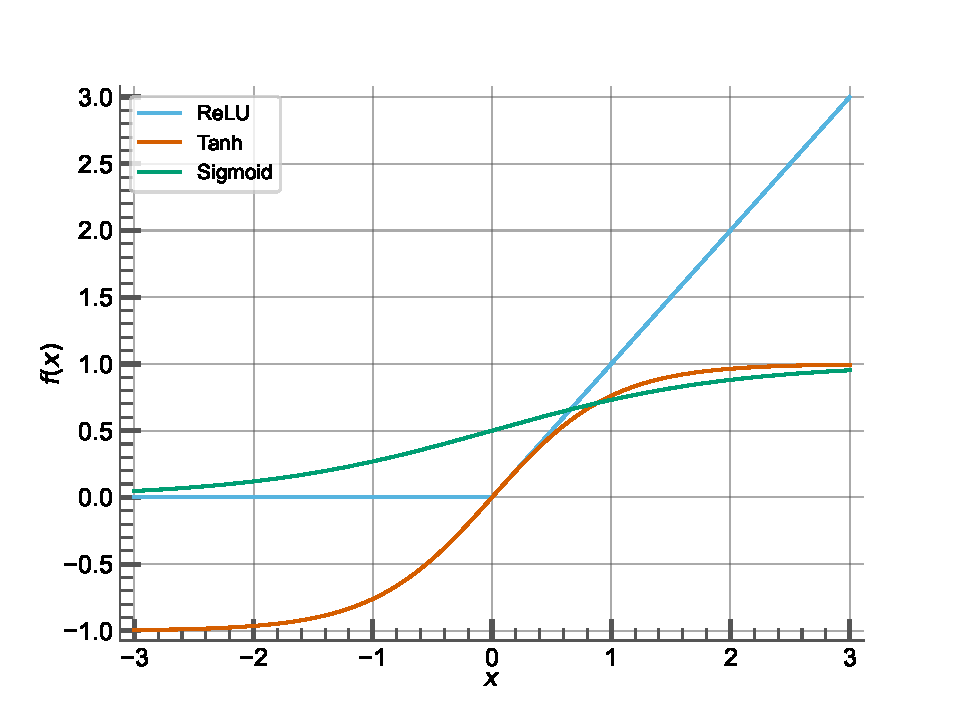
\includegraphics[width=0.7\textwidth]{chapter_dlo/assets/activation_functions.pdf}
  \caption{\ac{ReLU}, tanh and sigmoid activation functions.}
  \label{fig:dlo:activation_functions}
\end{figure}

\noindent \textbf{Pooling.} Pooling is often employed after \ac{CL} layers
in a \ac{CNN} and aims at progressively reducing the spatial size of the input
representation, thus reducing the number of parameters and computations in the
network. This also helps control overfitting and increases the receptive field
of the subsequent layers. The pooling operation is performed independently on
each input channel, so the depth dimension remains unchanged. The two most
common types of pooling are \emph{max pooling} and \emph{average pooling}. with
the former, the maximum value in each window (often of size $2\times 2$) is
selected, while the latter computes the average value of the window. Given an
input matrix $\mathbf{x}$ and a pooling function $p$, the output matrix $
\mathbf{y} $ for a certain spatial location $(i, j)$ is defined as follows:\\

\begin{equation}
  \label{eqn:dlo:pooling}
  y_{ij} = p \left( \mathbf{x}(i⋅s:i⋅s+f,j⋅s:j⋅s+f) \right)
\end{equation}\\

\noindent where $s$ is the stride or step size, $f$ is the spatial extent of the
filter, or window size and $\mathbf{x}(m:n)$ denotes a slice of the vector or
matrix $\mathbf{x}$ starting at index $m$ and ending at index $n$. Note that
pooling has no learnable parameters. They only downsample the input based on a
fixed function.\\


\noindent \textbf{Batch Normalisation.} \ac{BN} is a technique introduced in
\cite{DBLP:conf/icml/IoffeS15} to combat the issue of internal covariate shift
in deep neural networks, thereby accelerating training and improving
generalization. Covariate shift refers to the change in the input distribution
to a learning system, which can lead to slow convergence and make the network
harder to train. \ac{BN} normalises the input layer by adjusting and scaling the
activations. For each mini-batch, it computes the mean and variance of the
activations and performs normalization. The transformation is defined as
follows:\\

\begin{equation}
  \label{eqn:dlo:batchnorm}
  \hat{x}_{i} = \frac{x_{i} - \mu_{B}}{\sqrt{\sigma_{B}^{2} + \varepsilon}}
\end{equation}\\

\noindent where $x_{i}$ is the input, $\mu_{B}$ is the mini-batch mean,
$\sigma_{B}^{2}$ is the mini-batch variance, and $\varepsilon$ is a small
constant for numerical stability. After normalization, the method allows the
network to learn an affine transformation for each activation, permitting the
network to control the mean and standard deviation of the input distribution,
formalised in \cref{eqn:dlo:batchnorm}.\\

\begin{equation}
  \label{eqn:dlo:batchnorm_affine}
  y_{i} = \gamma \hat{x}_{i} + \beta
\end{equation}\\

\noindent where, $\gamma$ and $\beta$ are the learnable parameters of the affine
transformation. \ac{BN} has the advantage of making the network less sensitive
to the initial weights, allowing higher learning rates, and reducing the need
for Dropout, among other regularisers. However, its effectiveness decreases in
the case of small batch sizes, as the estimate of the batch mean and variance
becomes less accurate.\\

\noindent \textbf{Dropout.} Dropout is a regularization technique used to
prevent overfitting in neural networks. Dropout was introduced in
\cite{DBLP:journals/jmlr/SrivastavaHKSS14} and works by randomly deactivating a
proportion of neurons in a layer during each training iteration. More
specifically, during the forward pass, each neuron has a probability $p$ of
being temporarily removed from the network, effectively breaking up
co-adaptations between neurons and forcing them to learn more robust and
independent features (see \cref{eqn:dlo:dropout}).\\

\begin{equation}
  \label{eqn:dlo:dropout}
    r_i \sim \text{Bernoulli}(1 - p), \quad
    \mathbf{y} = \frac{\mathbf{x} \odot \mathbf{r}}{1 - p} 
\end{equation}\\

\noindent where $\mathbf{x}$ denote the output of a layer processed with
dropout, $\mathbf{r}$ is a binary mask vector of the same shape as $\mathbf{x}$,
where each element of $r$ is independently drawn from a Bernoulli distribution
with probability $1-p$, leading to $r_i=1$ if the associated weight is kept and
a $r_i=0$ if not. The product $\mathbf{x} \odot \mathbf{r}$ is scaled by $1-p$
to ensure that the expected value of $\mathbf{x}$ remains unchanged. During the
evaluation, the dropout is changed to an identity function.

\subsection{Architectures}\label{sec:dlo:architectures}


The evolution of \aclp{CNN} is characterized by a consistent increase in their
size and performance, alongside the introduction of new architectural
modifications to address the limitations of their predecessors (see
\cref{fig:dlo:net_sizes}). In this section, we present a historical overview of
the \acp{CNN} evolution and we subsequently detail the architectures that we
used in our experiments.\\

The first \ac{CNN} was introduced in 1998: LeNet-5 was developed for digit
recognition \cite{DBLP:journals/pieee/LeCunBBH98}, constituting a relatively
simple network with 5 layers with learnable parameters: 2 \ac{CL} layers
and 3 fully connected layers. Its size is significantly smaller compared to the
contemporary models (see \cref{fig:dlo:net_sizes}). With the introduction of
AlexNet \cite{DBLP:conf/nips/KrizhevskySH12} in 2012, the network size
considerably grew, comprising more layers and neurons to handle more complex
tasks, like large-scale image recognition. AlexNet tackled the overfitting issue
in LeNet-5 with the use of data augmentation and dropout techniques and
introduced and popularised the \ac{ReLU} activation function.\\

\begin{figure}[htbp]
  \centering
  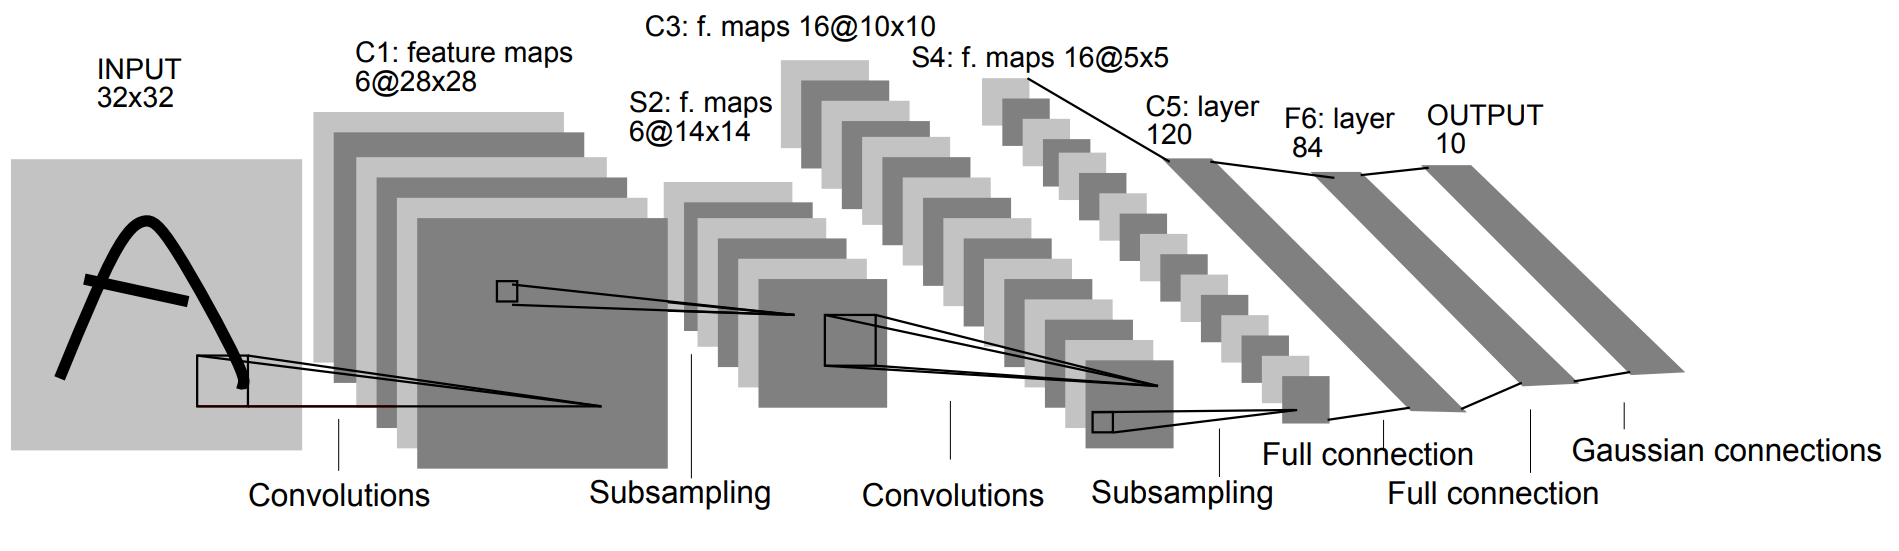
\includegraphics[width=0.70\textwidth]{chapter_sota/assets/lenet.png}
  \caption{Architecture of LeNet-5, a \acl{CNN} used for handwritten digit
    recognition. Image taken from \cite{DBLP:journals/pieee/LeCunBBH98}}
  \label{fig:dlo:lenet5}
\end{figure}


The next advancement was the VGG networks family
\cite{DBLP:journals/corr/SimonyanZ14a} %, introduced in 2014 
which proposed much deeper architectures with up to 19 layers, which is a
significant increase over the 8 layers of AlexNet. However, the increased depth
led to the \emph{vanishing gradients} problems. The vanishing gradients problem
refers to the situation in training a deep neural network where gradients are
backpropagated through layers and become increasingly small, effectively
preventing the weights of earlier layers from learning and updating effectively.
The VGG networks also introduced the practice of stacking multiple convolutional
layers with small $3\times 3$ filters instead of using larger filters. The same
year, Google's Inception (or GoogLeNet) \cite{DBLP:conf/cvpr/SzegedyLJSRAEVR15}
was introduced, addressing the vanishing gradients  issue with its novel
inception modules, which allowed the network to learn at varying scales and
increased computational efficiency, without overly increasing the network size.
GoogleNet was also the first \ac{CNN} that was not a simple stack of layers and
processed a single input with different blocks in parallel before merging
them.\\

\begin{figure}[htbp]
  \centering
  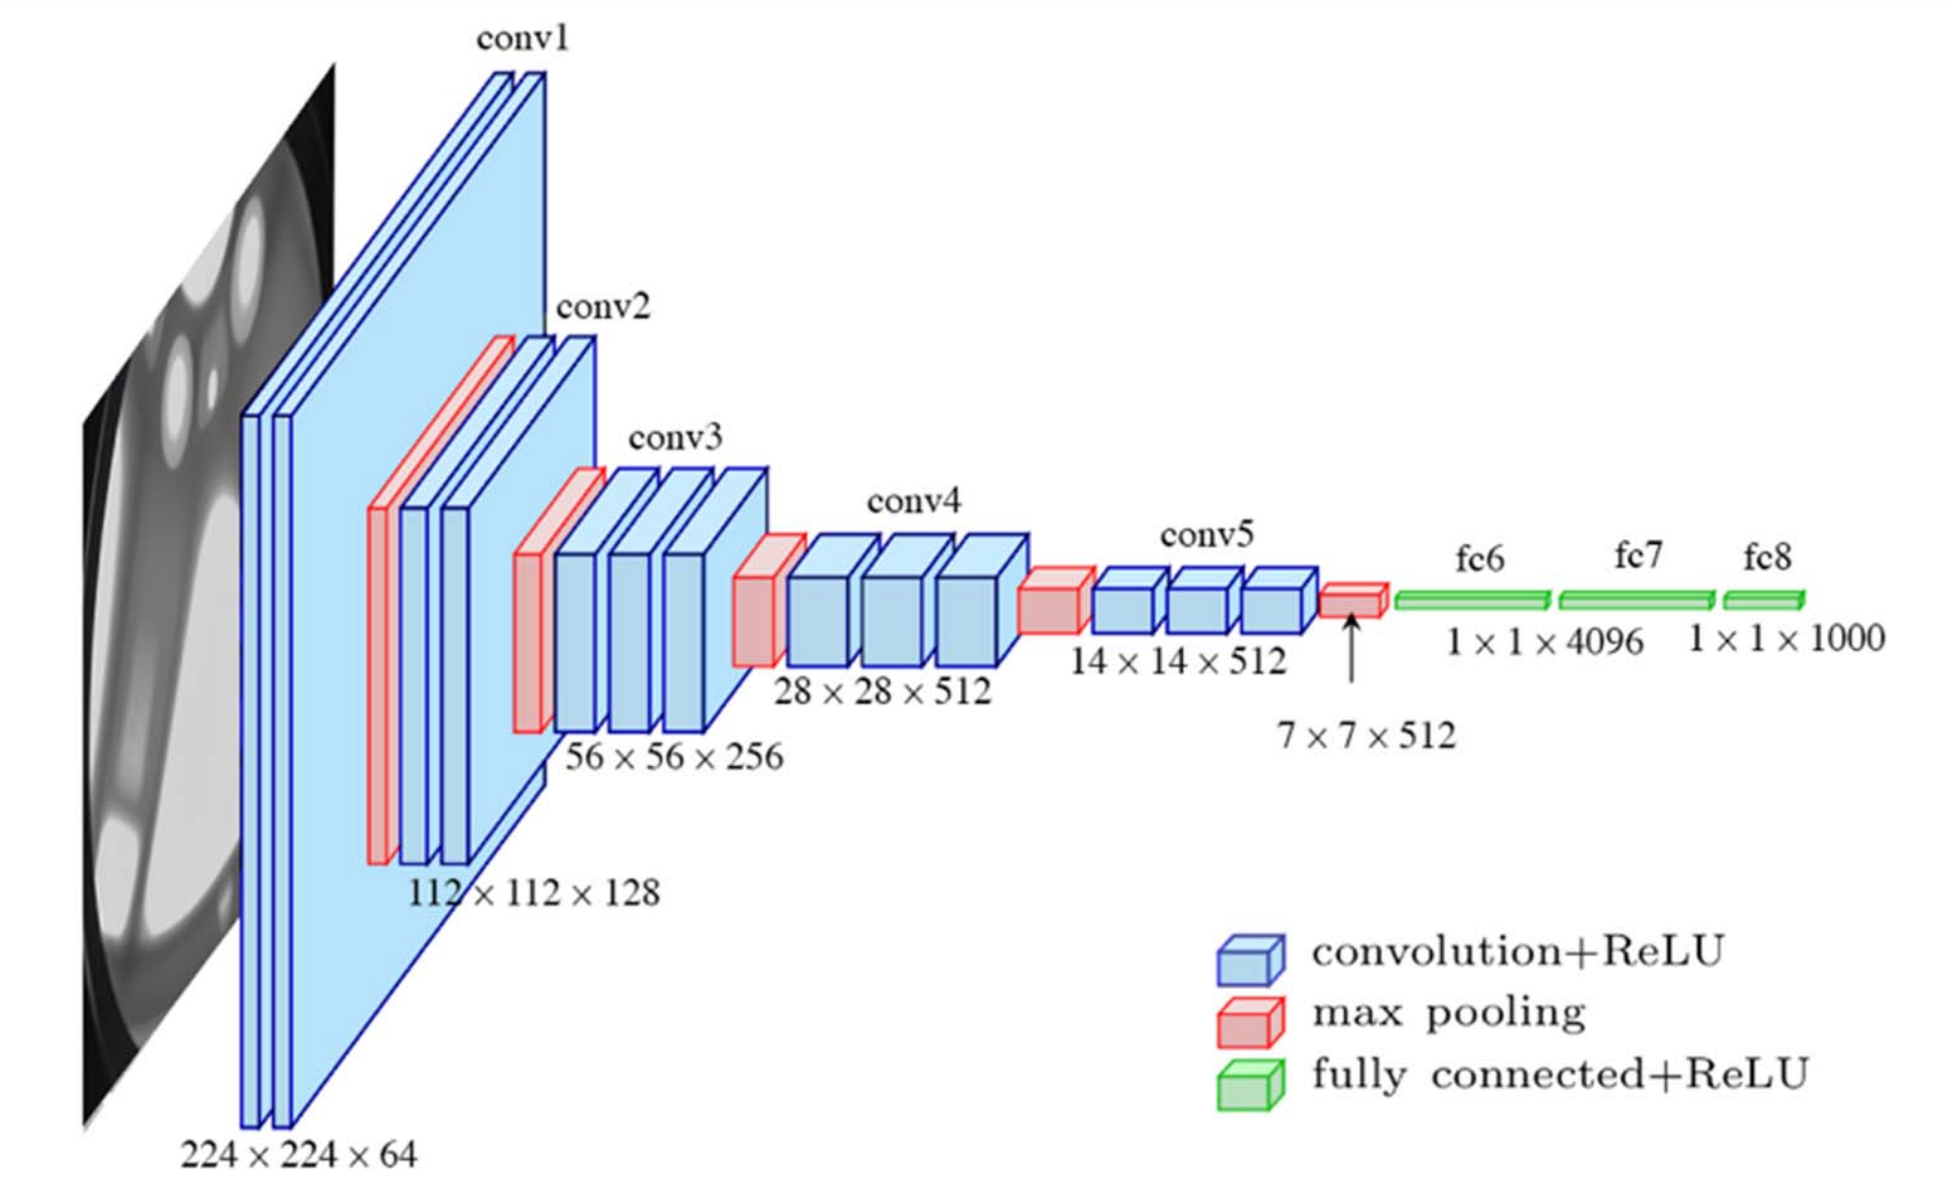
\includegraphics[width=0.7\textwidth]{chapter_sota/assets/vgg16.png}
  \caption{Architecture of the VGG16 network introduced in
    \cite{DBLP:journals/corr/SimonyanZ14a}. Image taken from
    \cite{ferguson2017automatic}}
  \label{fig:dlo:vgg16}
\end{figure}

Later, the ResNet models family was proposed in \cite{DBLP:conf/cvpr/HeZRS16},
which effectively tackled the vanishing gradient problem by introducing skip (or
shortcut) connections, allowing gradients to backpropagate directly through
several layers. These shortcut connections also allowed the network to grow in
depth up to 152 layers without a significant increase in computational cost.
However, a challenge remained with the constant need for careful design to
manage feature-map sizes.\\

\begin{figure}[htbp]
  \centering
  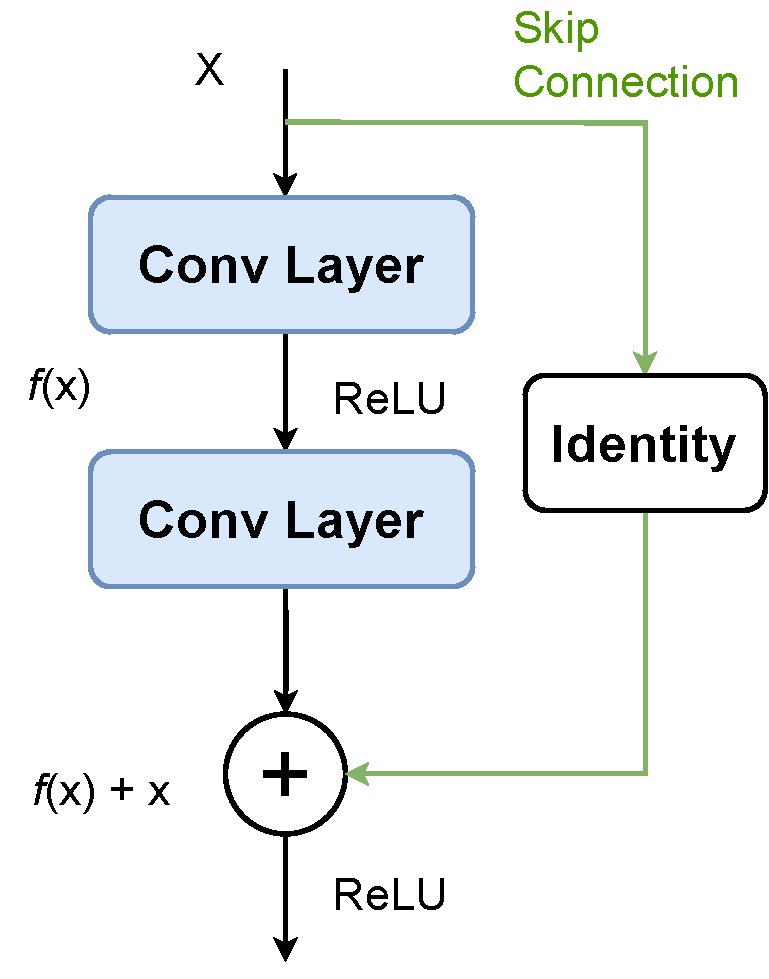
\includegraphics[width=0.5\textwidth]{chapter_dlo/assets/skip_connection.pdf}
  \caption{A residual block and its skip connection used in
    ResNets\cite{DBLP:conf/cvpr/HeZRS16}. The identity skip connection allows
    for the gradient to be backpropagated directly through several layers, thus
    mitigating the \emph{vanishing gradients} problem.}
  \label{fig:dlo:skip_connection}
\end{figure}

In response, DenseNet \cite{huang2017densely} was proposed. It connects each
layer to every other following layer of the same block in a feed-forward
fashion. By reinforcing the propagation of features and gradients through the
network, DenseNet alleviated the vanishing-gradient problem and further improved
the ability of the network to pass on information from earlier layers to later
ones. Thus, through these chronological advancements, neural networks not only
grew in size but also improved in performance, thereby becoming more efficient
and capable of handling more complex tasks.\\

\begin{figure}[htbp]
  \centering
  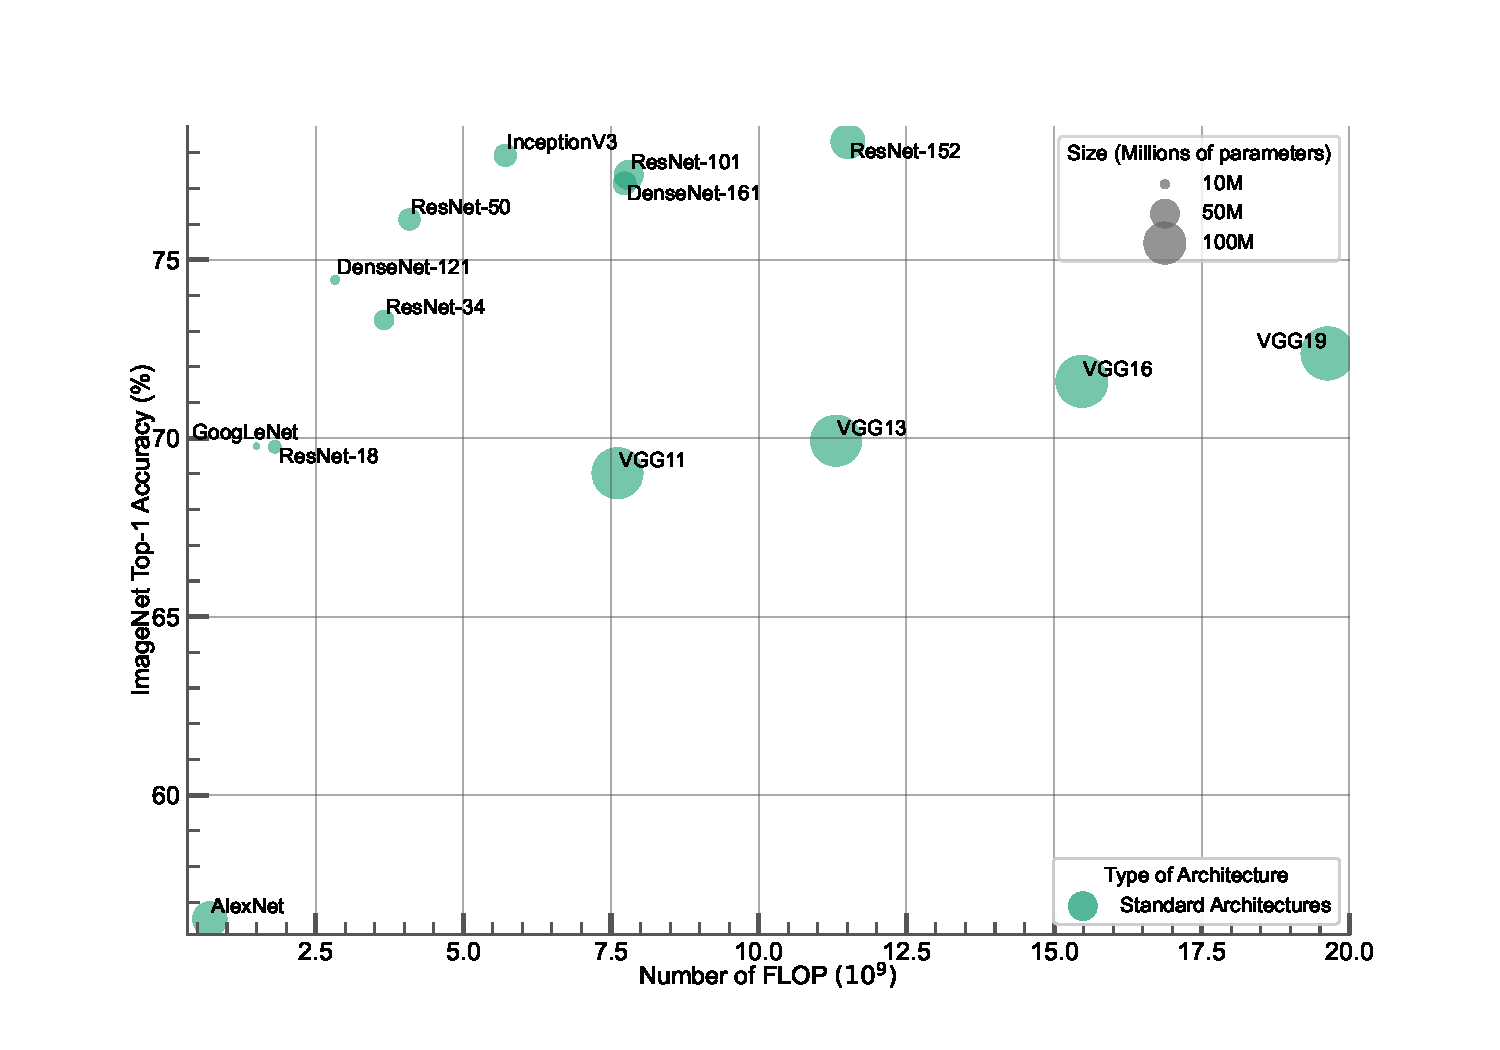
\includegraphics[width=0.7\textwidth]{chapter_sota/assets/network_sizes_normal.pdf}
  \caption{Networks size comparison. The \emph{x-axis} represents the number of
    \acp{FLOP} required to process a single image. The \emph{y-axis} represents
    the Top-1 accuracy on the ImageNet \cite{deng2009imagenet} dataset and the
    size of the circles represents the number of parameters in the network.
    Numbers are taken from \cite{pytorch_vision}}
  \label{fig:dlo:net_sizes}
\end{figure}

In the subsequent paragraphs, we detail the architectures that we used in our
experiments. We chose these architectures because they are representative of the
state-of-the-art in image classification and they are widely used in the pruning
literature. \Cref{tab:dlo:networks_size} gives an overview of the different
network architectures.\\

\begin{table}[ht!]
  \centering
  \begin{tabular}{lcccccc}
    \cline{2-7}
    & \textbf{Conv2} & \textbf{Conv4} & \textbf{Conv6} & \textbf{VGG16} & \textbf{ResNet20} & \textbf{ResNet18} \\ \hline
    Number of Parameters & 4,301,642 & 2,425,930  & 2,262,602      & 14,728,266
    & 269,034           & 11,685,608 \\
    Number of layers & 5 & 7 & 9 & 14 & 20 & 18 \\
    Number of \ac{CL} layers & 2 & 4 & 6 & 13 & 19 & 17 \\
    Number of \ac{FC} layers & 3 & 3 & 3 & 1 & 1 & 1 \\ \hline
  \end{tabular}
  \caption{Number of parameters for the used neural network architectures. The
  number of parameters is given for the CIFAR-10 dataset, except for the
  ResNet18 architecture, whose number of parameters is given for the
  TinyImageNet dataset.}
  \label{tab:dlo:networks_size}
\end{table}

% VGG16
\noindent \textbf{VGG16.} The VGG16 network
\cite{DBLP:journals/corr/SimonyanZ14a} is a 16-layer \ac{CNN} composed of 13
\ac{CL} layers and 3 fully connected layers. VGG16 was originally deseign
for ImageNet \cite{deng2009imagenet} and in our experiments with CIFAR-10 and
CIFAR-100 (described in \cref{sec:dlo:datasets}) we use a slightly modified
version of VGG16 where we replace the 3 \ac{FC} layers with an average pooling
layer and a single \ac{FC} layer \cite{vggcifar}. The \ac{CL} layers
filters are of size $3\times 3$ with a stride of 1. The max-pooling layers are
of size $2\times 2$ with a stride of 2. Each \ac{CL} layer is followed by
a \ac{ReLU} activation function. The VGG16 network is illustrated in
\cref{fig:dlo:vgg16_cifar}.\\

\begin{figure}[htbp]
  \centering
  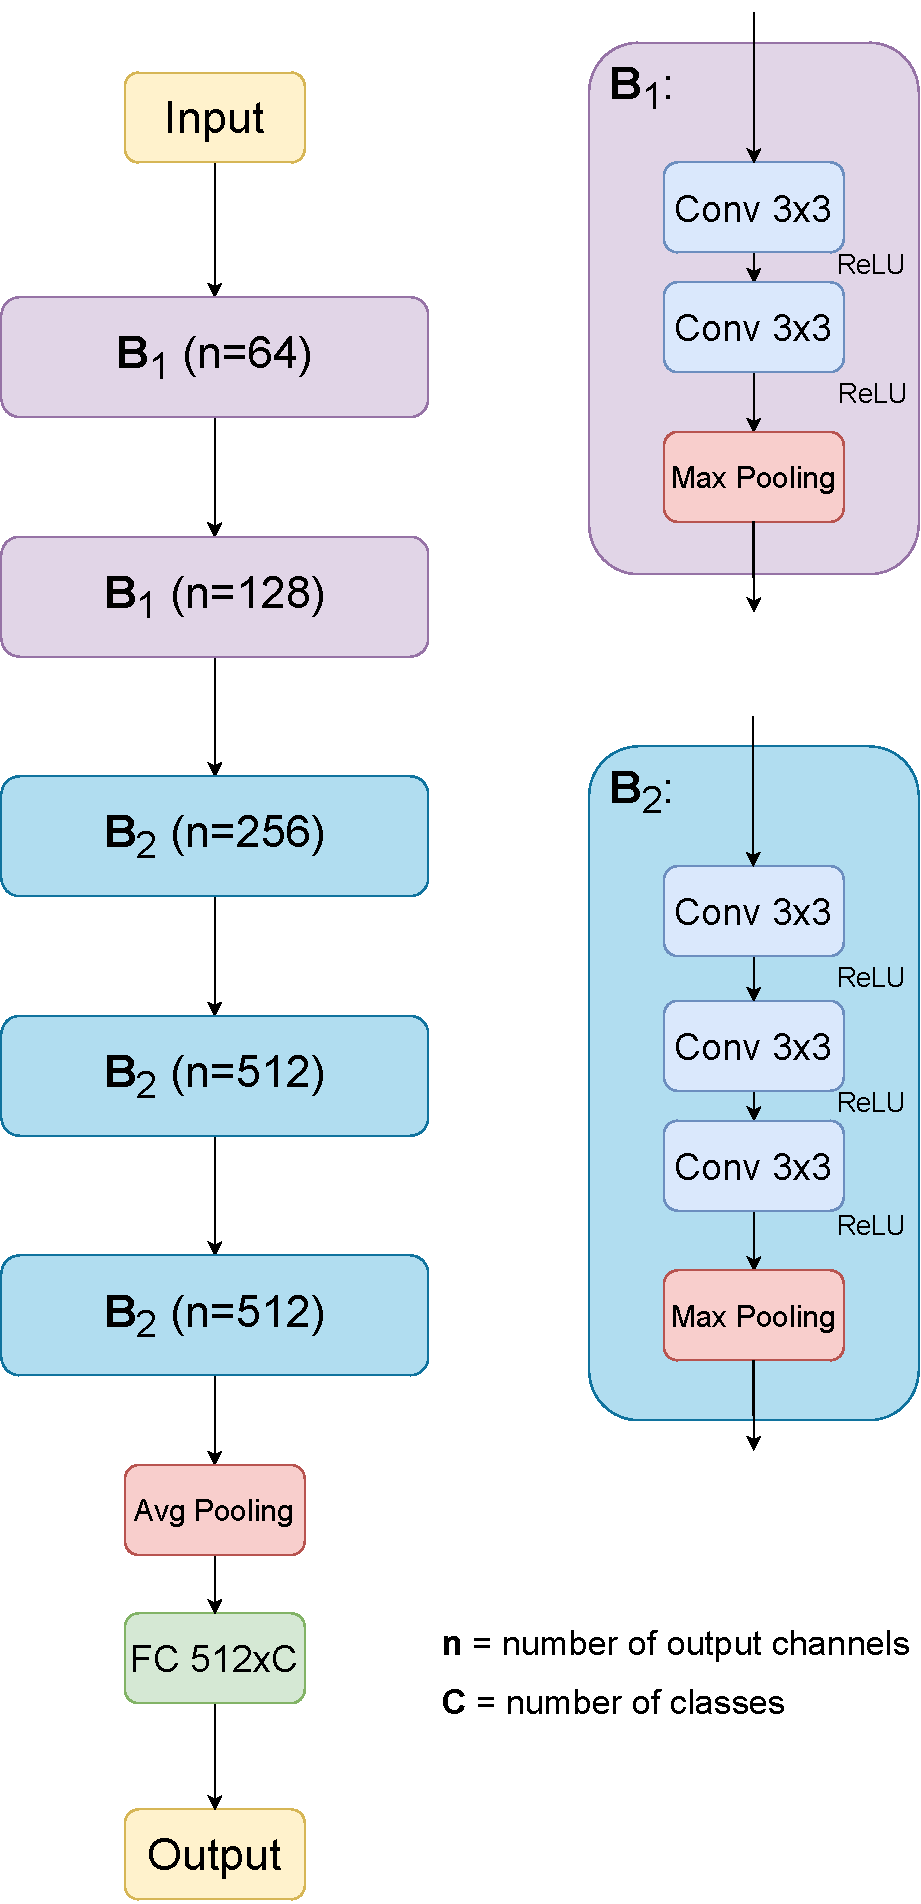
\includegraphics[width=0.30\textwidth]{chapter_dlo/assets/vgg16_cifar.pdf}
  \caption{VGG16 adapted for CIFAR-10 and CIFAR-100.}
  \label{fig:dlo:vgg16_cifar}
\end{figure}

% ResNet18 and ResNet20
\noindent \textbf{ResNet\{18,20\}.} The ResNet18 and ResNet20 networks
\cite{DBLP:conf/cvpr/HeZRS16} are 18 and 20-layer \acp{CNN} respectively. These
layers are organized into stages, with ResNet18, represented in
\cref{fig:dlo:resnet18}, consisting of 4 stages with 2 \ac{CL} layers each,
while ResNet20, represented in \cref{fig:dlo:resnet20}, is structured into 3
stages, each containing 3 \ac{CL} layers. They are composed of \emph{Residual
Blocks} also referred to as \emph{Basic Blocks}. Each residual block follows the
principle of learning the residual function:\\

\begin{equation}
  f(x) = h(x) - x
\end{equation} \\

\noindent where $h(x)$ is the mapping usually learned by previous architectures
such as VGG16. The representation of a residual block is given by
\cref{eqn:dlo:residual_block} (see also \cref{fig:dlo:skip_connection}): \\

\begin{equation}
  \label{eqn:dlo:residual_block}
  y = f(x,\theta) + x
\end{equation}\\

\noindent where $x$ is the input, $f$ represents the residual function, $\theta$
are the weights of the block, and $y$ is the output. In
\cref{eqn:dlo:residual_block} $+ x$ denotes the skip connection, which enables
direct backpropagation of the gradient to earlier layers.\\

\begin{figure}
\centering
\subfloat[ResNet20\label{fig:dlo:resnet20}]{
  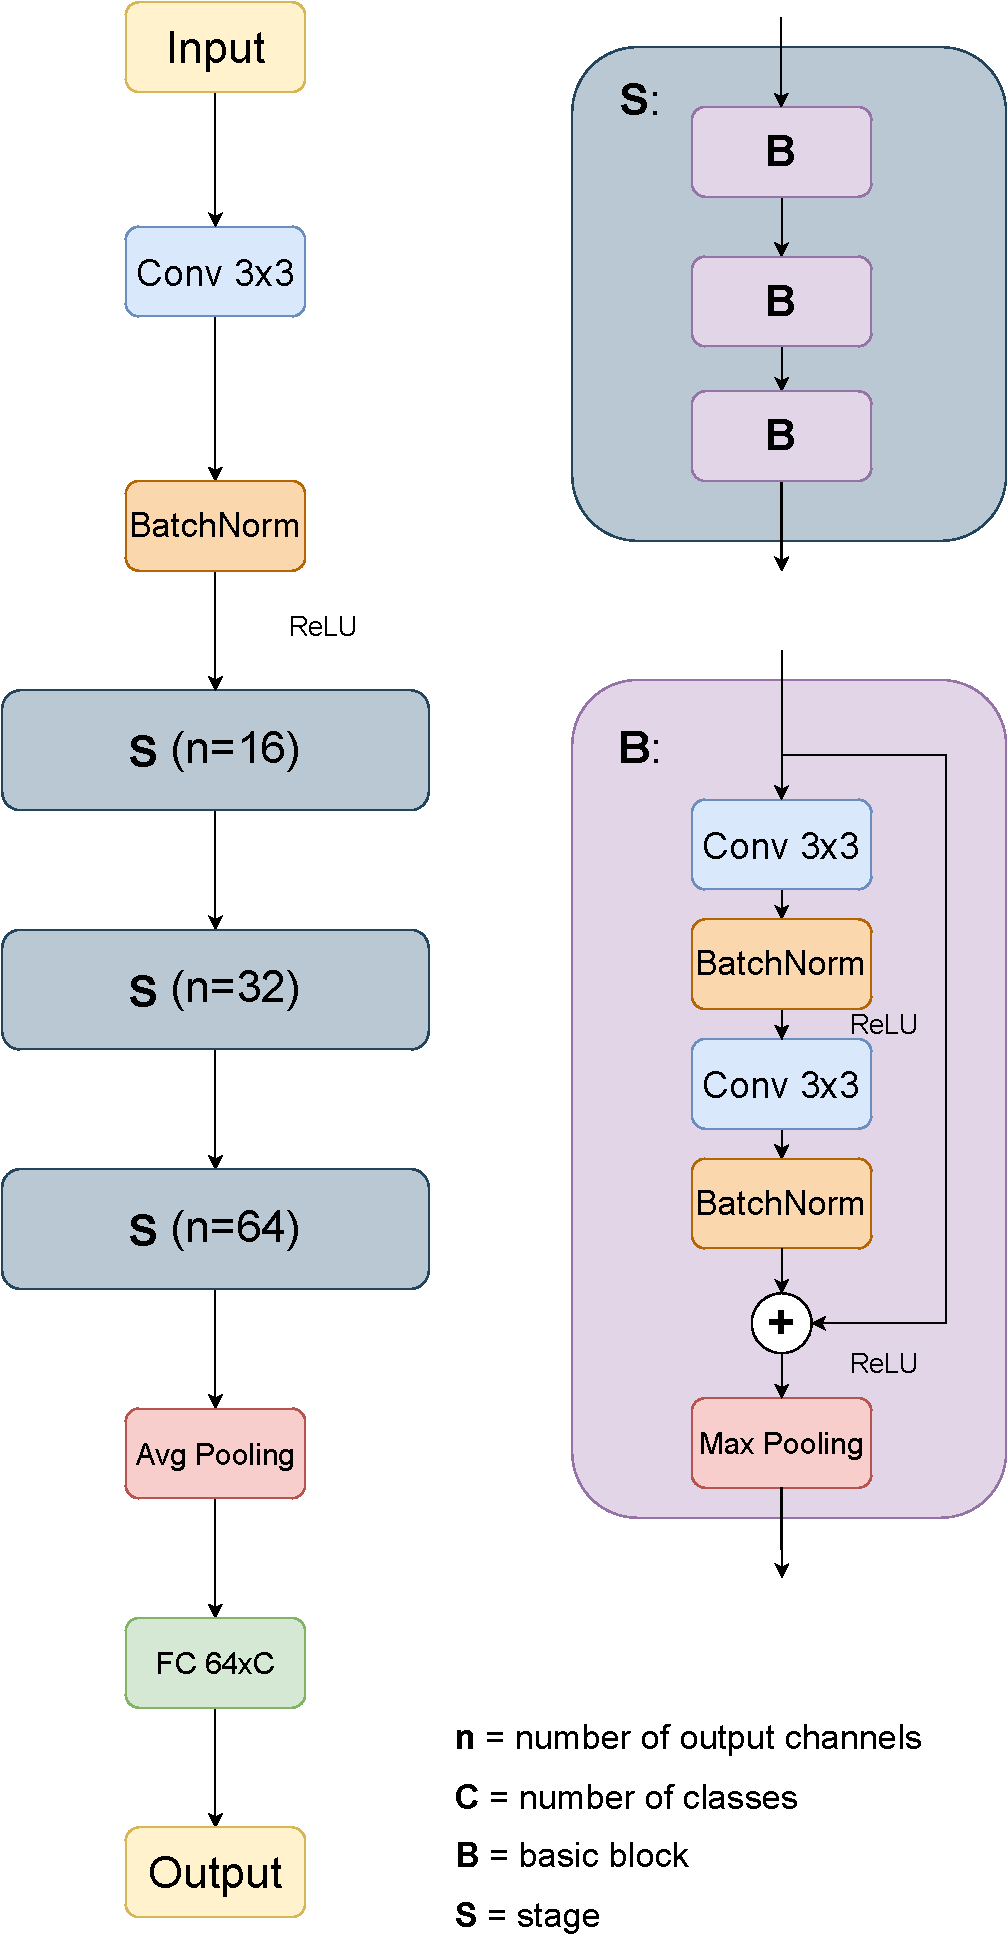
\includegraphics[width=0.35\textwidth]{chapter_dlo/assets/resnet20.pdf}}
  \hfill
\subfloat[ResNet18\label{fig:dlo:resnet18}]{
  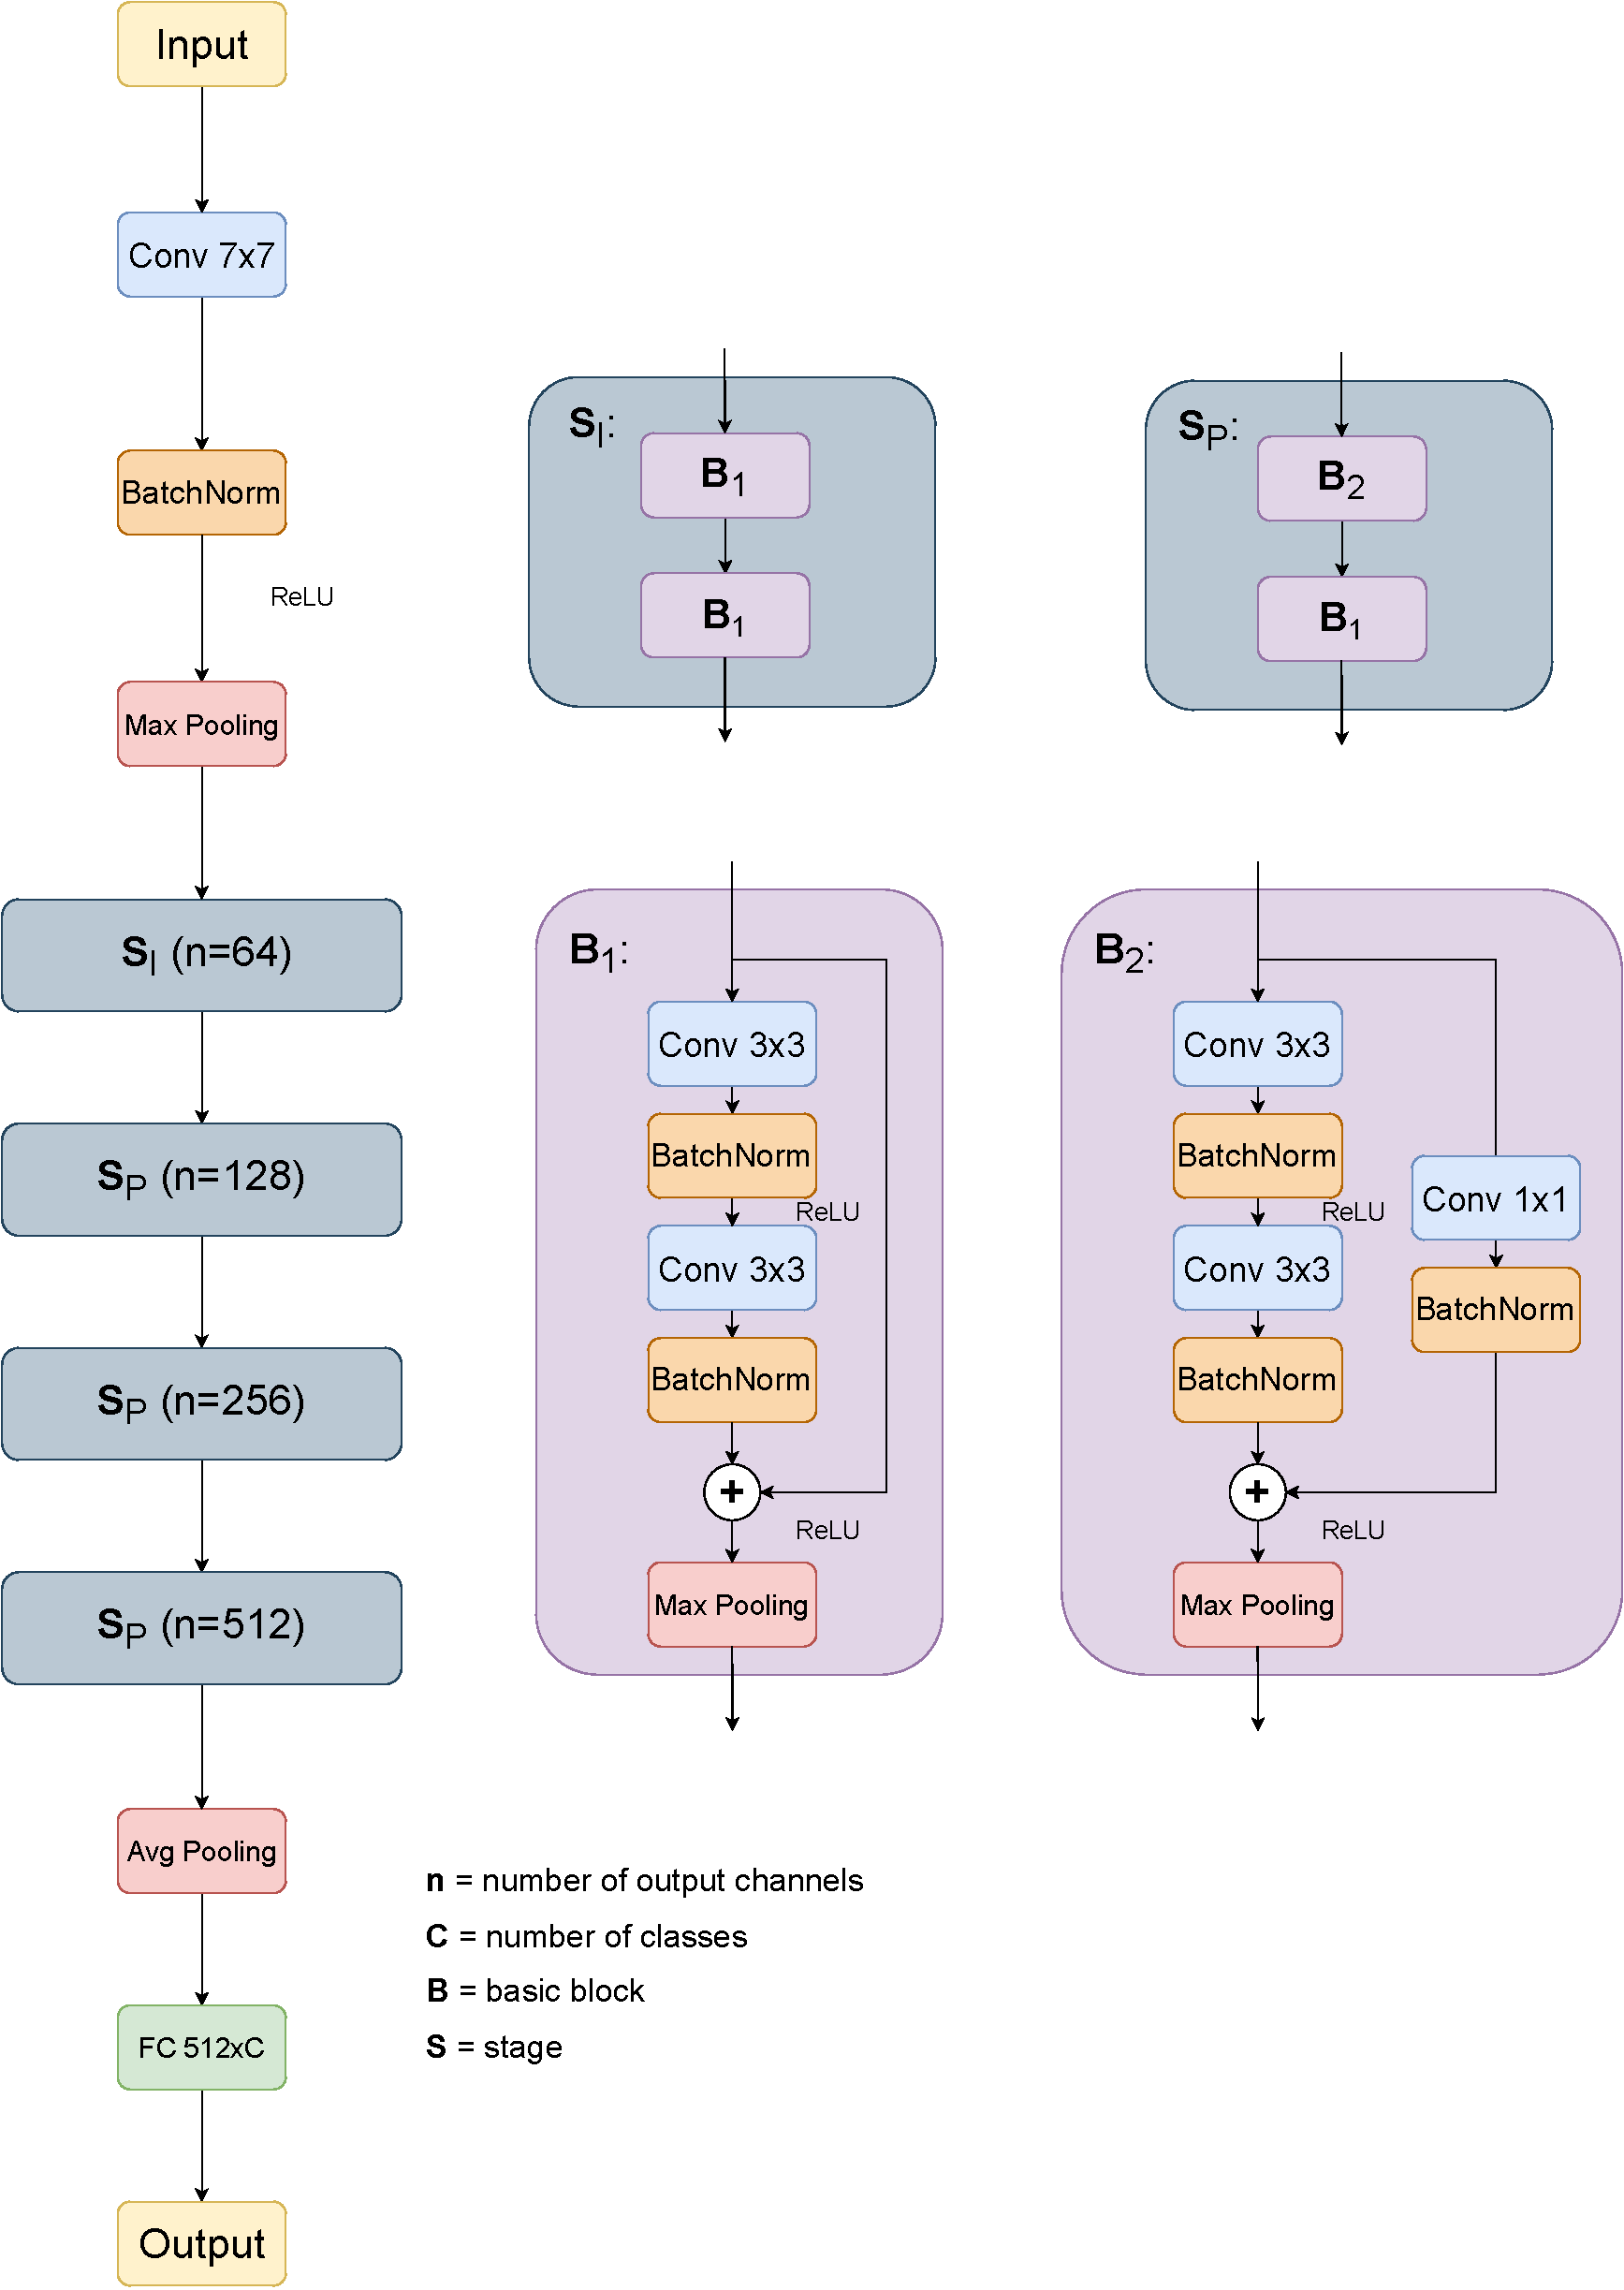
\includegraphics[width=0.60\textwidth]{chapter_dlo/assets/resnet18.pdf}}

\caption{ResNet20 and ResNet18 architectures. ResNet20 (\cref{fig:dlo:resnet20})
is tailored for CIFAR-10 and comprises 3 stages encompassing 3 \emph{Basic
Blocks} of 2 \ac{CL} layers each, with an identity skip connection in each
block. ResNet18 (\cref{fig:dlo:resnet18}) is tailored for ImageNet and is
composed of 4 stages encompassing 4 \emph{Basic Blocks} of 2 convolutional
layers each. There are two types of blocks: $\mathbf{B}_\text{I}$ with an
identity skip connection and $\mathbf{B}_\text{P}$ with a projection skip
connection. The projection skip connection is used to match the dimensions
between the input and the output of the block.}
\label{fig:dlo:resnets}
\end{figure}

\noindent \textbf{Conv\{2,4,6\}.} The Conv2, Conv4 and Conv6 networks are shrunk
down versions of the VGG16 network, composed of 2, 4 and 6 \ac{CL} layers
respectively and 3 \ac{FC} layers. Although the Conv2, Conv4 and Conv6 networks
introduced by \citeauthor{DBLP:conf/iclr/FrankleC19} in
\cite{DBLP:conf/iclr/FrankleC19} are not widely featured in existing literature,
we chose to employ them due to their use in the methods we benchmark against.
The \ac{CL} layers are stacked in increasing depth, and their
convolutional filters are of size $3\times 3$ with a stride of 1. The
max-pooling layers are of size $2\times 2$ with a stride of 2. They are
represented in \cref{fig:dlo:conv246}.\\

\begin{figure}[htbp]
  \centering
  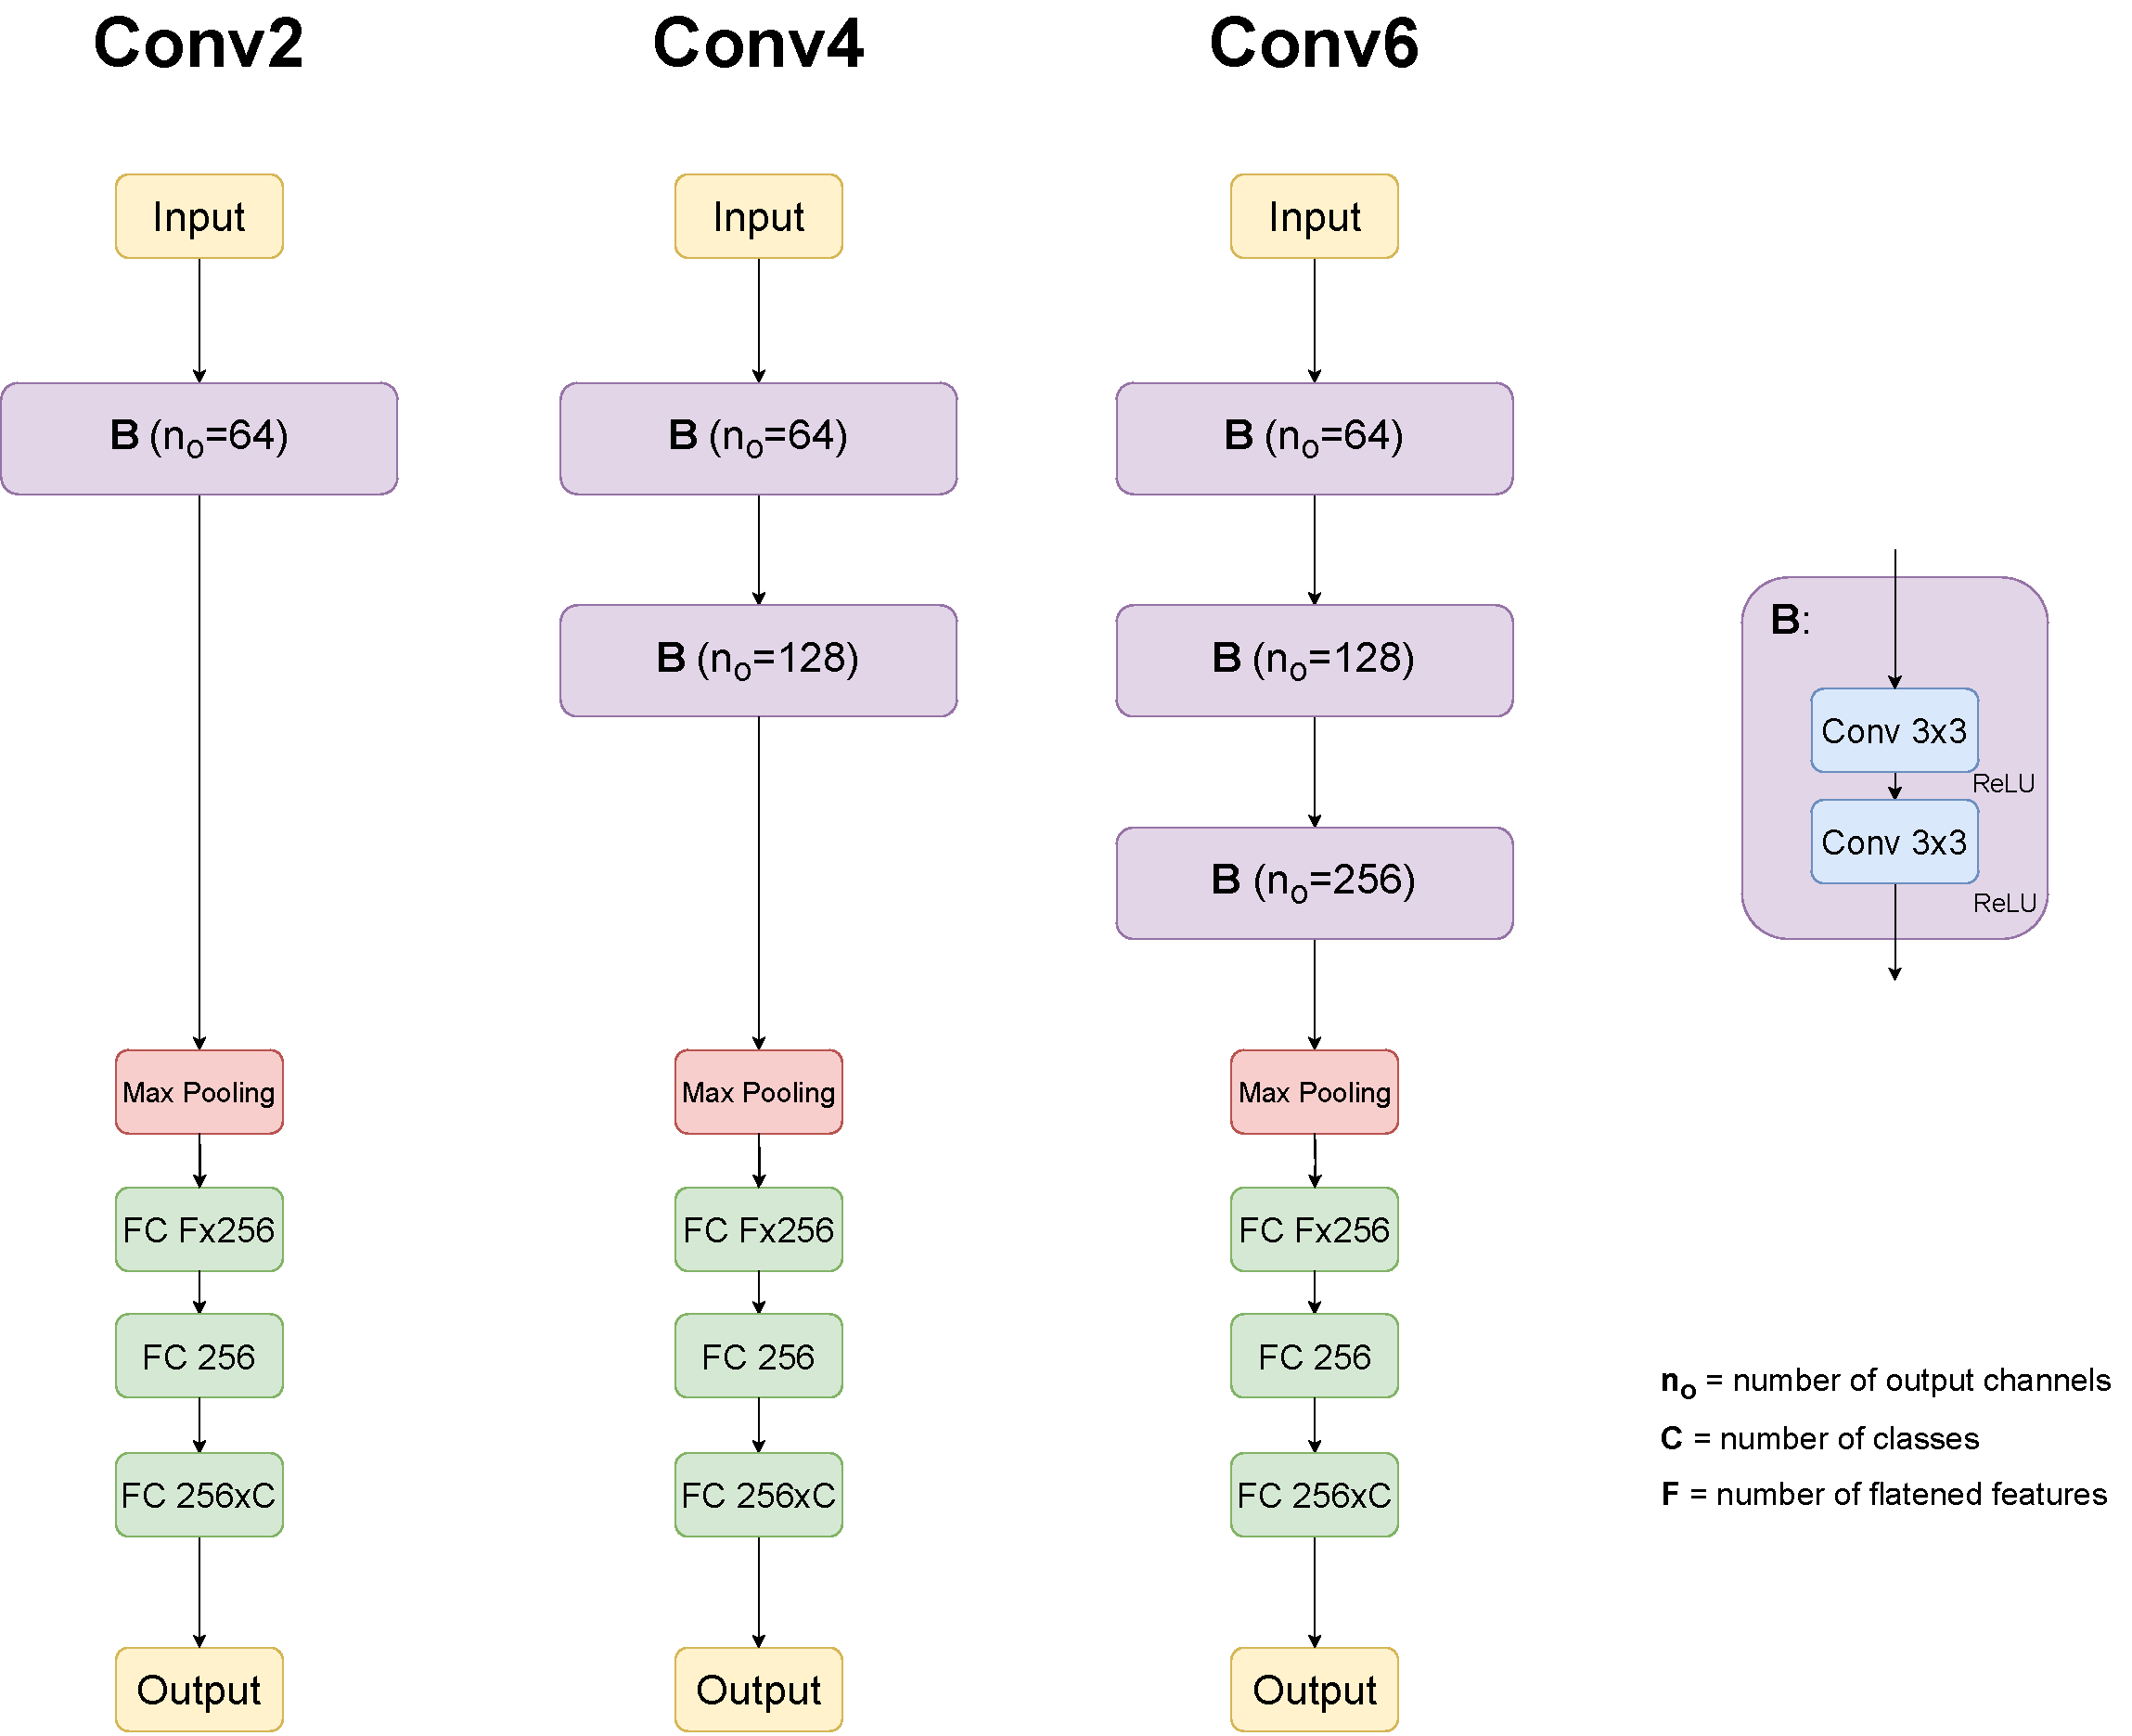
\includegraphics[width=0.7\textwidth]{chapter_dlo/assets/conv246.pdf}
  \caption{Conv2, Conv4 and Conv6 architectures. The number of flat features
  $\mathbf{F}$ corresponds to the size of the feature map of the last block
  $\mathbf{B}$, once vectorised. $\mathbf{F}=16384, ~8192~ \text{and}~ 4096$ for Conv2, Conv4
  and Conv6, respectively for input images of size $32\times 32$.}
  \label{fig:dlo:conv246}
\end{figure}


\section{Datasets}\label{sec:dlo:datasets}

In this thesis manuscript, we focus on image classification tasks and supervised
learning. Supervised learning is a machine learning paradigm in which the model
is trained using labeled data. In the context of image classification, the input
data is an image, and the label is the class of the image. We denote an input
image $X$ and its corresponding label $y$. Each image $X$ belongs to the set of
all images of the dataset $\mathcal{X}$, and each label $y$ belongs to the set
of all labels of the dataset $\mathcal{Y}$. The dataset, denoted $\mathcal{D}$,
is a set of pairs $(X, y)$, where $X \in \mathcal{X}$ and $y \in \mathcal{Y}$,
so that $D \subset \mathcal{X} \times \mathcal{Y}$. \\

In our experiments, we evaluated our methods on three different datasets
tailored for image classification: CIFAR-10 \cite{CIFARdataset}, CIFAR-100
\cite{CIFARdataset} and TinyImageNet \cite{TinyImageNet}. The following
paragraphs give details about these datasets and \cref{tab:dlo:datasets} sums
up their main characteristics.\\

\begin{table}[ht!]
  \centering
  \begin{tabular}{lcccc}
    \toprule
    \textbf{Dataset}    & \textbf{Number of images} & \textbf{Number of classes} &
    \textbf{Image size} & \textbf{Size of test set}                                               \\
    \hline
    CIFAR-10            & 60,000                    & 10                         & 32x32 & 10,000 \\
    CIFAR-100           & 60,000                    & 100                        & 32x32 & 10,000 \\
    TinyImageNet        & 100,000                   & 200                        & 64x64 & 10,000 \\
    \bottomrule
  \end{tabular}
  \caption{The number of images, of classes, image size and size of the test
    set for the three datasets used: CIFAR-10, CIFAR-100 and TinyImageNet.}
  \label{tab:dlo:datasets}
\end{table}

\subsection{CIFAR-10}

The CIFAR-10 dataset \cite{CIFARdataset} is a widely used dataset in machine
learning and computer vision. This is a labeled subset of the \emph{80 Million
Tiny Images} dataset \cite{4531741}. CIFAR-10 is a simple yet challenging
dataset that allows for quicker iteration or hyperparameter tuning than larger
datasets such as ImageNet \cite{DBLP:journals/ijcv/RussakovskyDSKS15}, but it is
significantly more complex than the MNIST dataset \cite{6296535}, which contains
grayscale handwritten digits images. the CIFAR-10 dataset contains 60,000 colour
images of size 32x32 pixels, split into 10 classes, namely: plane, car, bird,
cat, deer, dog, horse, ship, and truck. Each class contains 6,000 images. The
dataset is divided into two sets: a training set, composed of 50,000 images and
a test set containing 10,000 of them.\\

\begin{figure}[ht!]
  \centering
  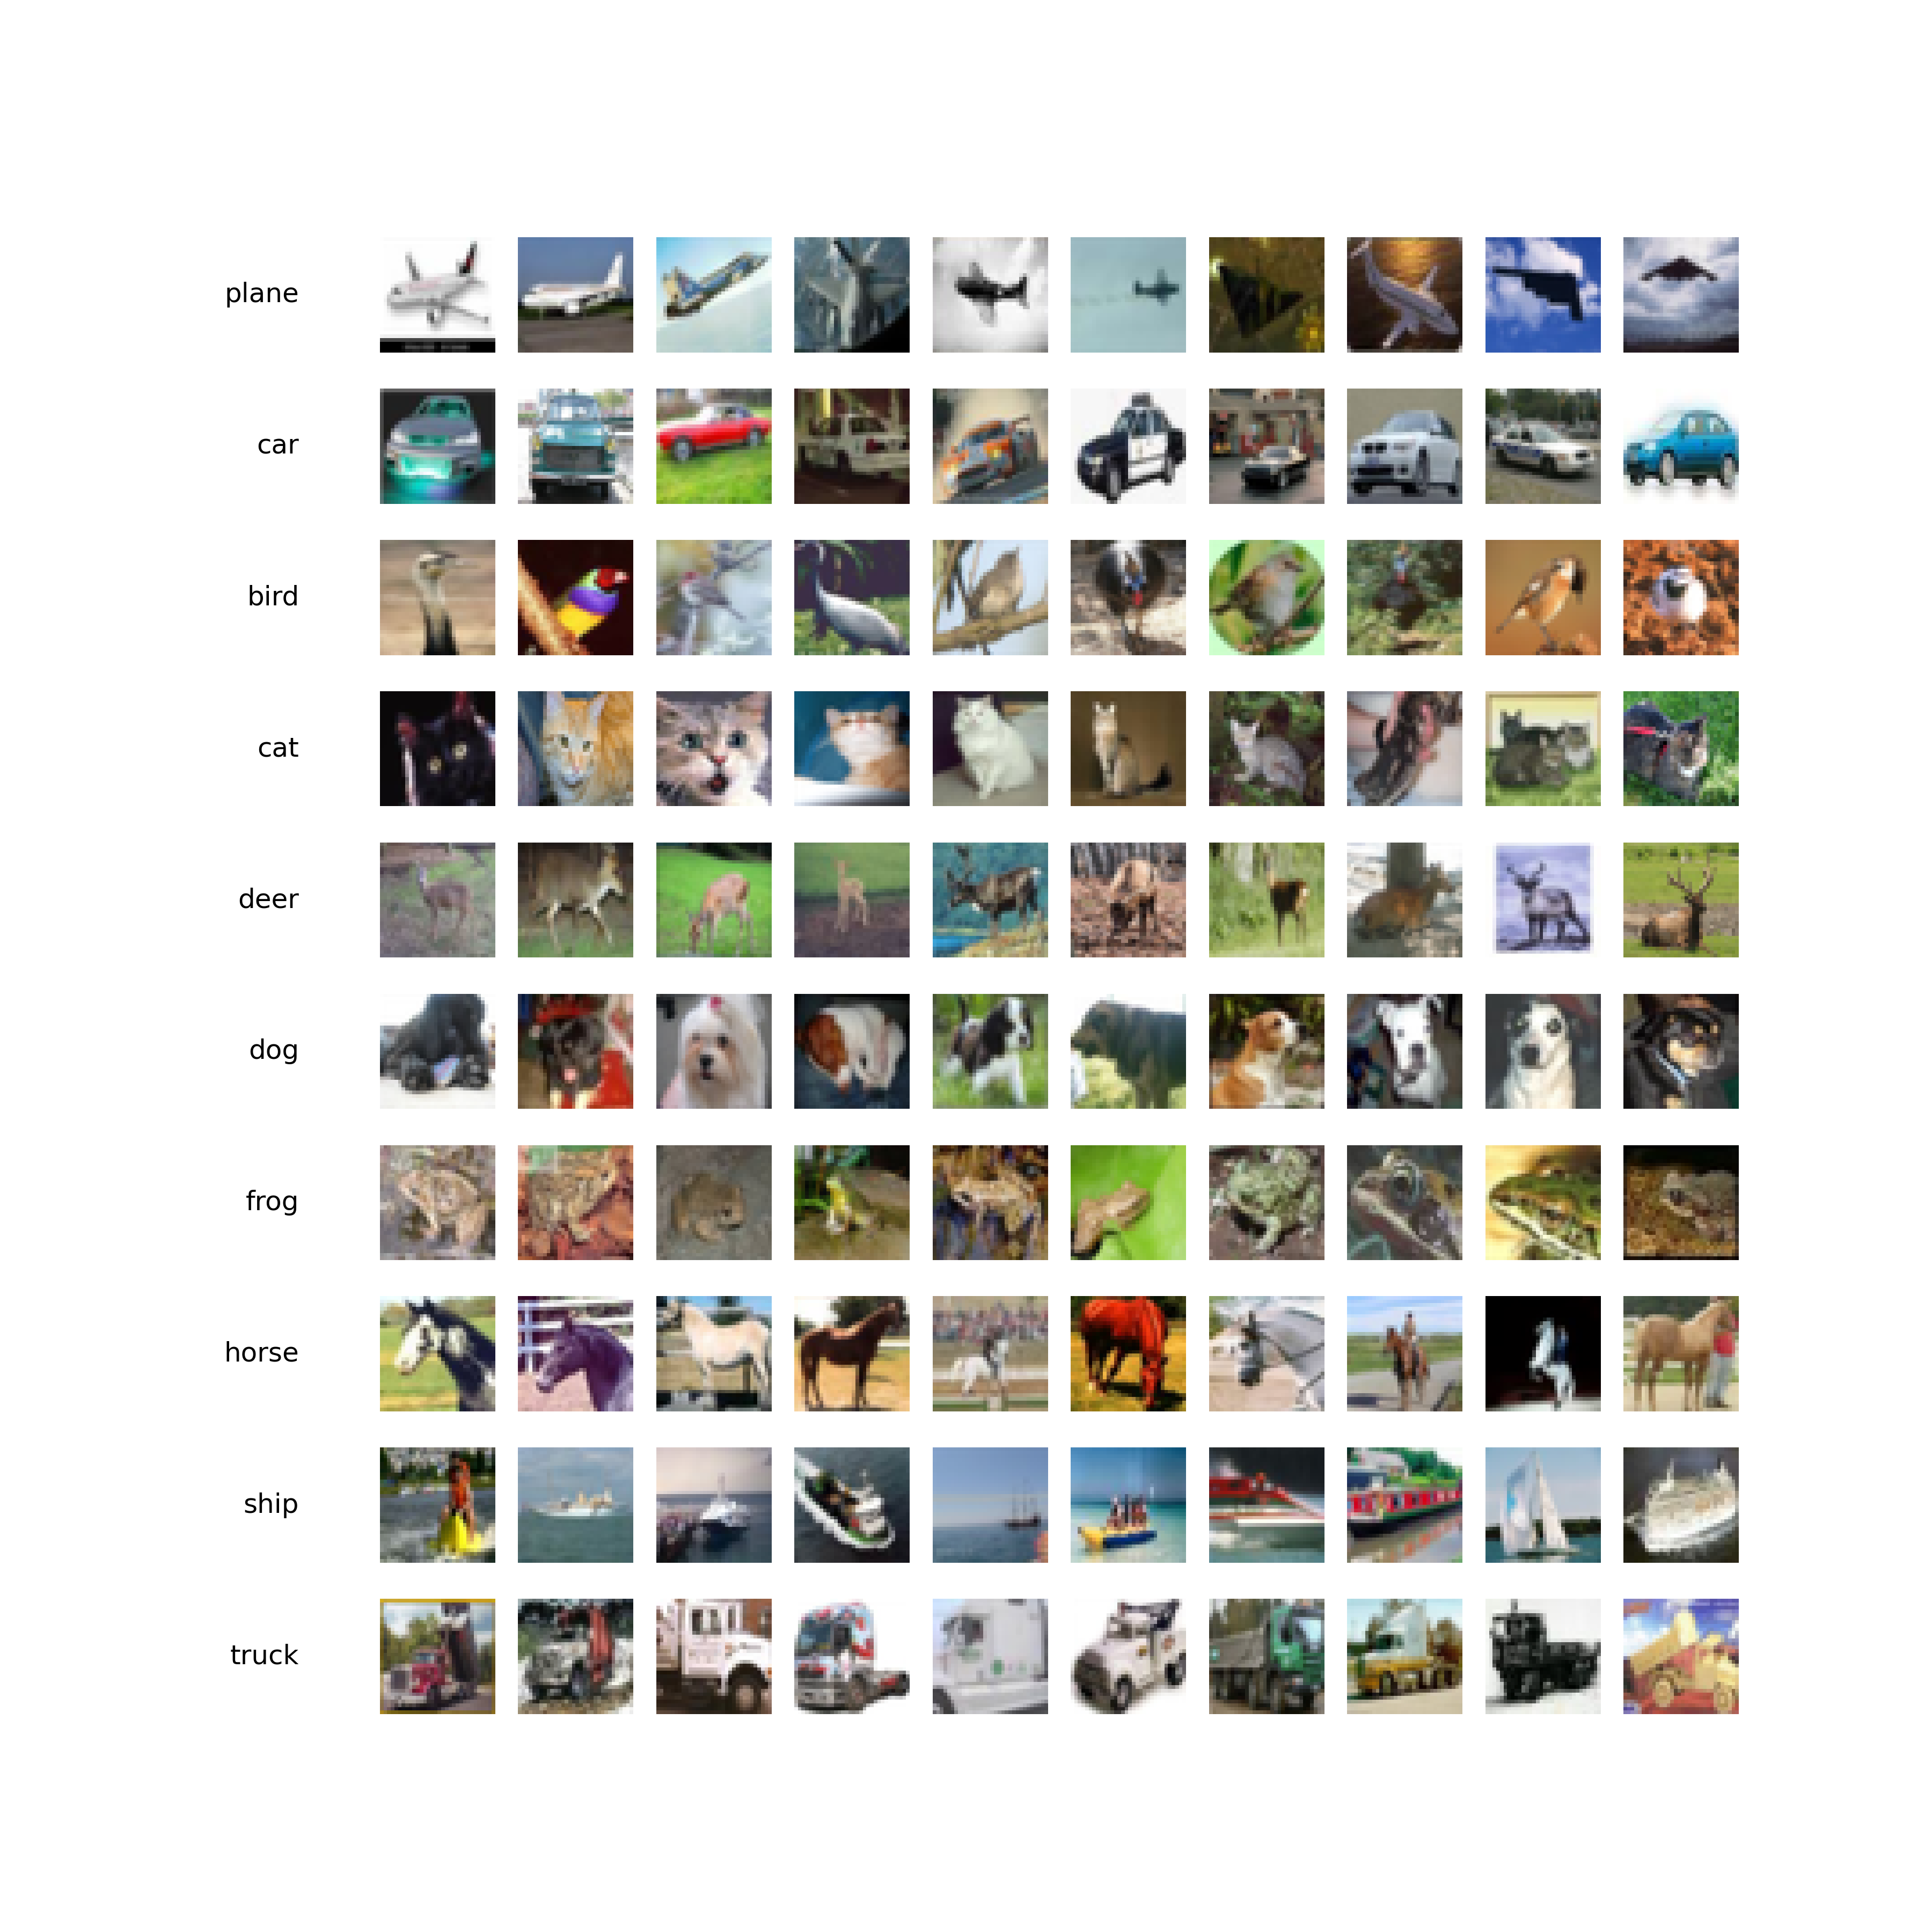
\includegraphics[width=0.7\textwidth]{chapter_dlo/assets/cifar-10_example.png}
  \caption{ A sample grid of images from the CIFAR-10 dataset. Each row
    contains images from one of the 10 classes: plane, car, bird, cat,
    deer, dog, frog, horse, ship, and truck}
  \label{fig:intro:cifar10_examples}
\end{figure}


\subsection{CIFAR-100}

CIFAR-100 \cite{CIFARdataset} is a more challenging
version of CIFAR-10. Like the latter, it is a labeled subset of the \emph{80
  Millions Tiny Images} and  is composed of 60,000 colour images of size 32x32
pixels. However, instead of 10 classes, CIFAR-100 contains 100 classes of 600
images each. As a result, each class has far fewer images than in CIFAR-10.
CIFAR-100 is also divided into two sets: a training set and a test, composed of
50,000 and 10,000 images respectively.\\

\begin{figure}[ht!]
  \centering
  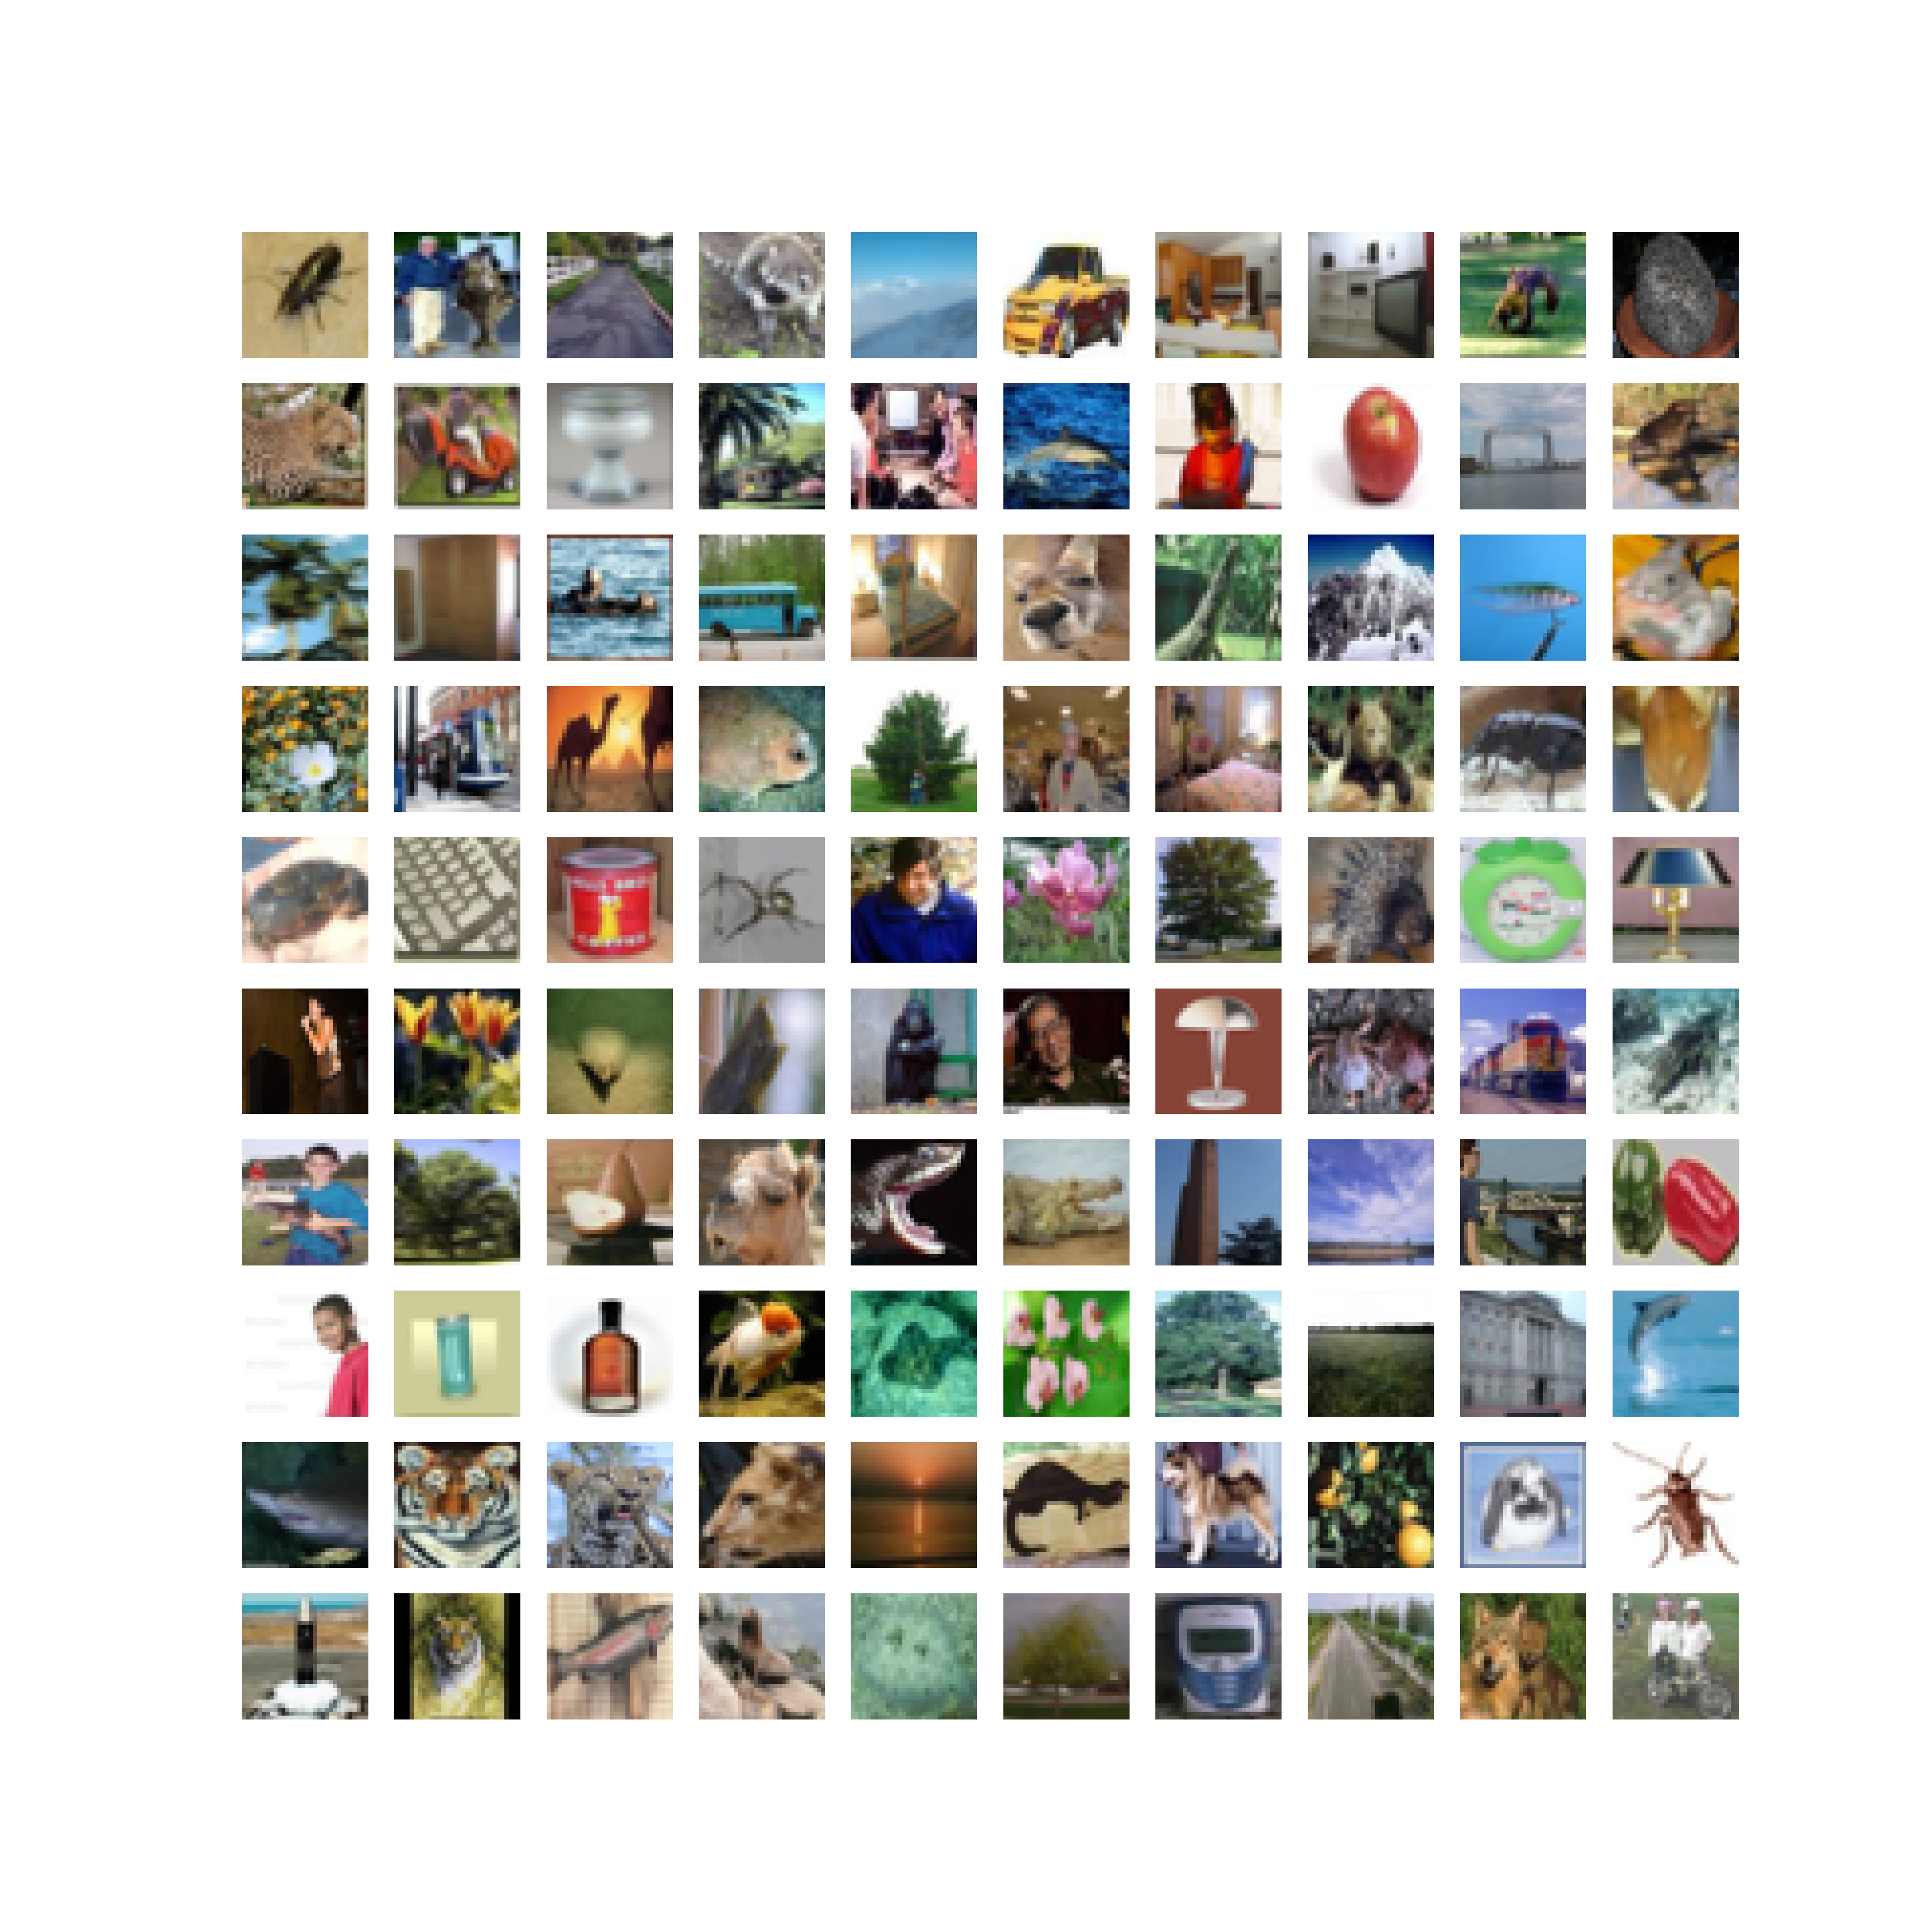
\includegraphics[width=0.7\textwidth]{chapter_dlo/assets/cifar-100_example.png}
  \caption{A sample grid of images from the CIFAR-100 dataset. The images
    represent a subset of the 100 available classes, each image represents
    a unique class.}
  \label{fig:intro:cifar100_examples}
\end{figure}


\subsection{TinyImageNet}

TinyImageNet dataset is another popular dataset in machine learning and computer
vision, conceived as a subset of the larger ImageNet dataset
\cite{DBLP:journals/ijcv/RussakovskyDSKS15}. It comprises 100,000 colour images
of size 64x64 pixels, split into 200 classes, whereas ImageNet contains 1.2
million images of size 256x256 pixels, split into 1,000 classes. The dataset is
divided in 3 sets: the train set, which contains 500 images per class, the
validation and test sets, which both contain 50. The scaled-down image size and
count make TinyImageNet more computationally accessible than ImageNet while
still being a challenging task and maintaining the diversity of the images and
classes.\\


\begin{figure}[ht!]
  \centering
  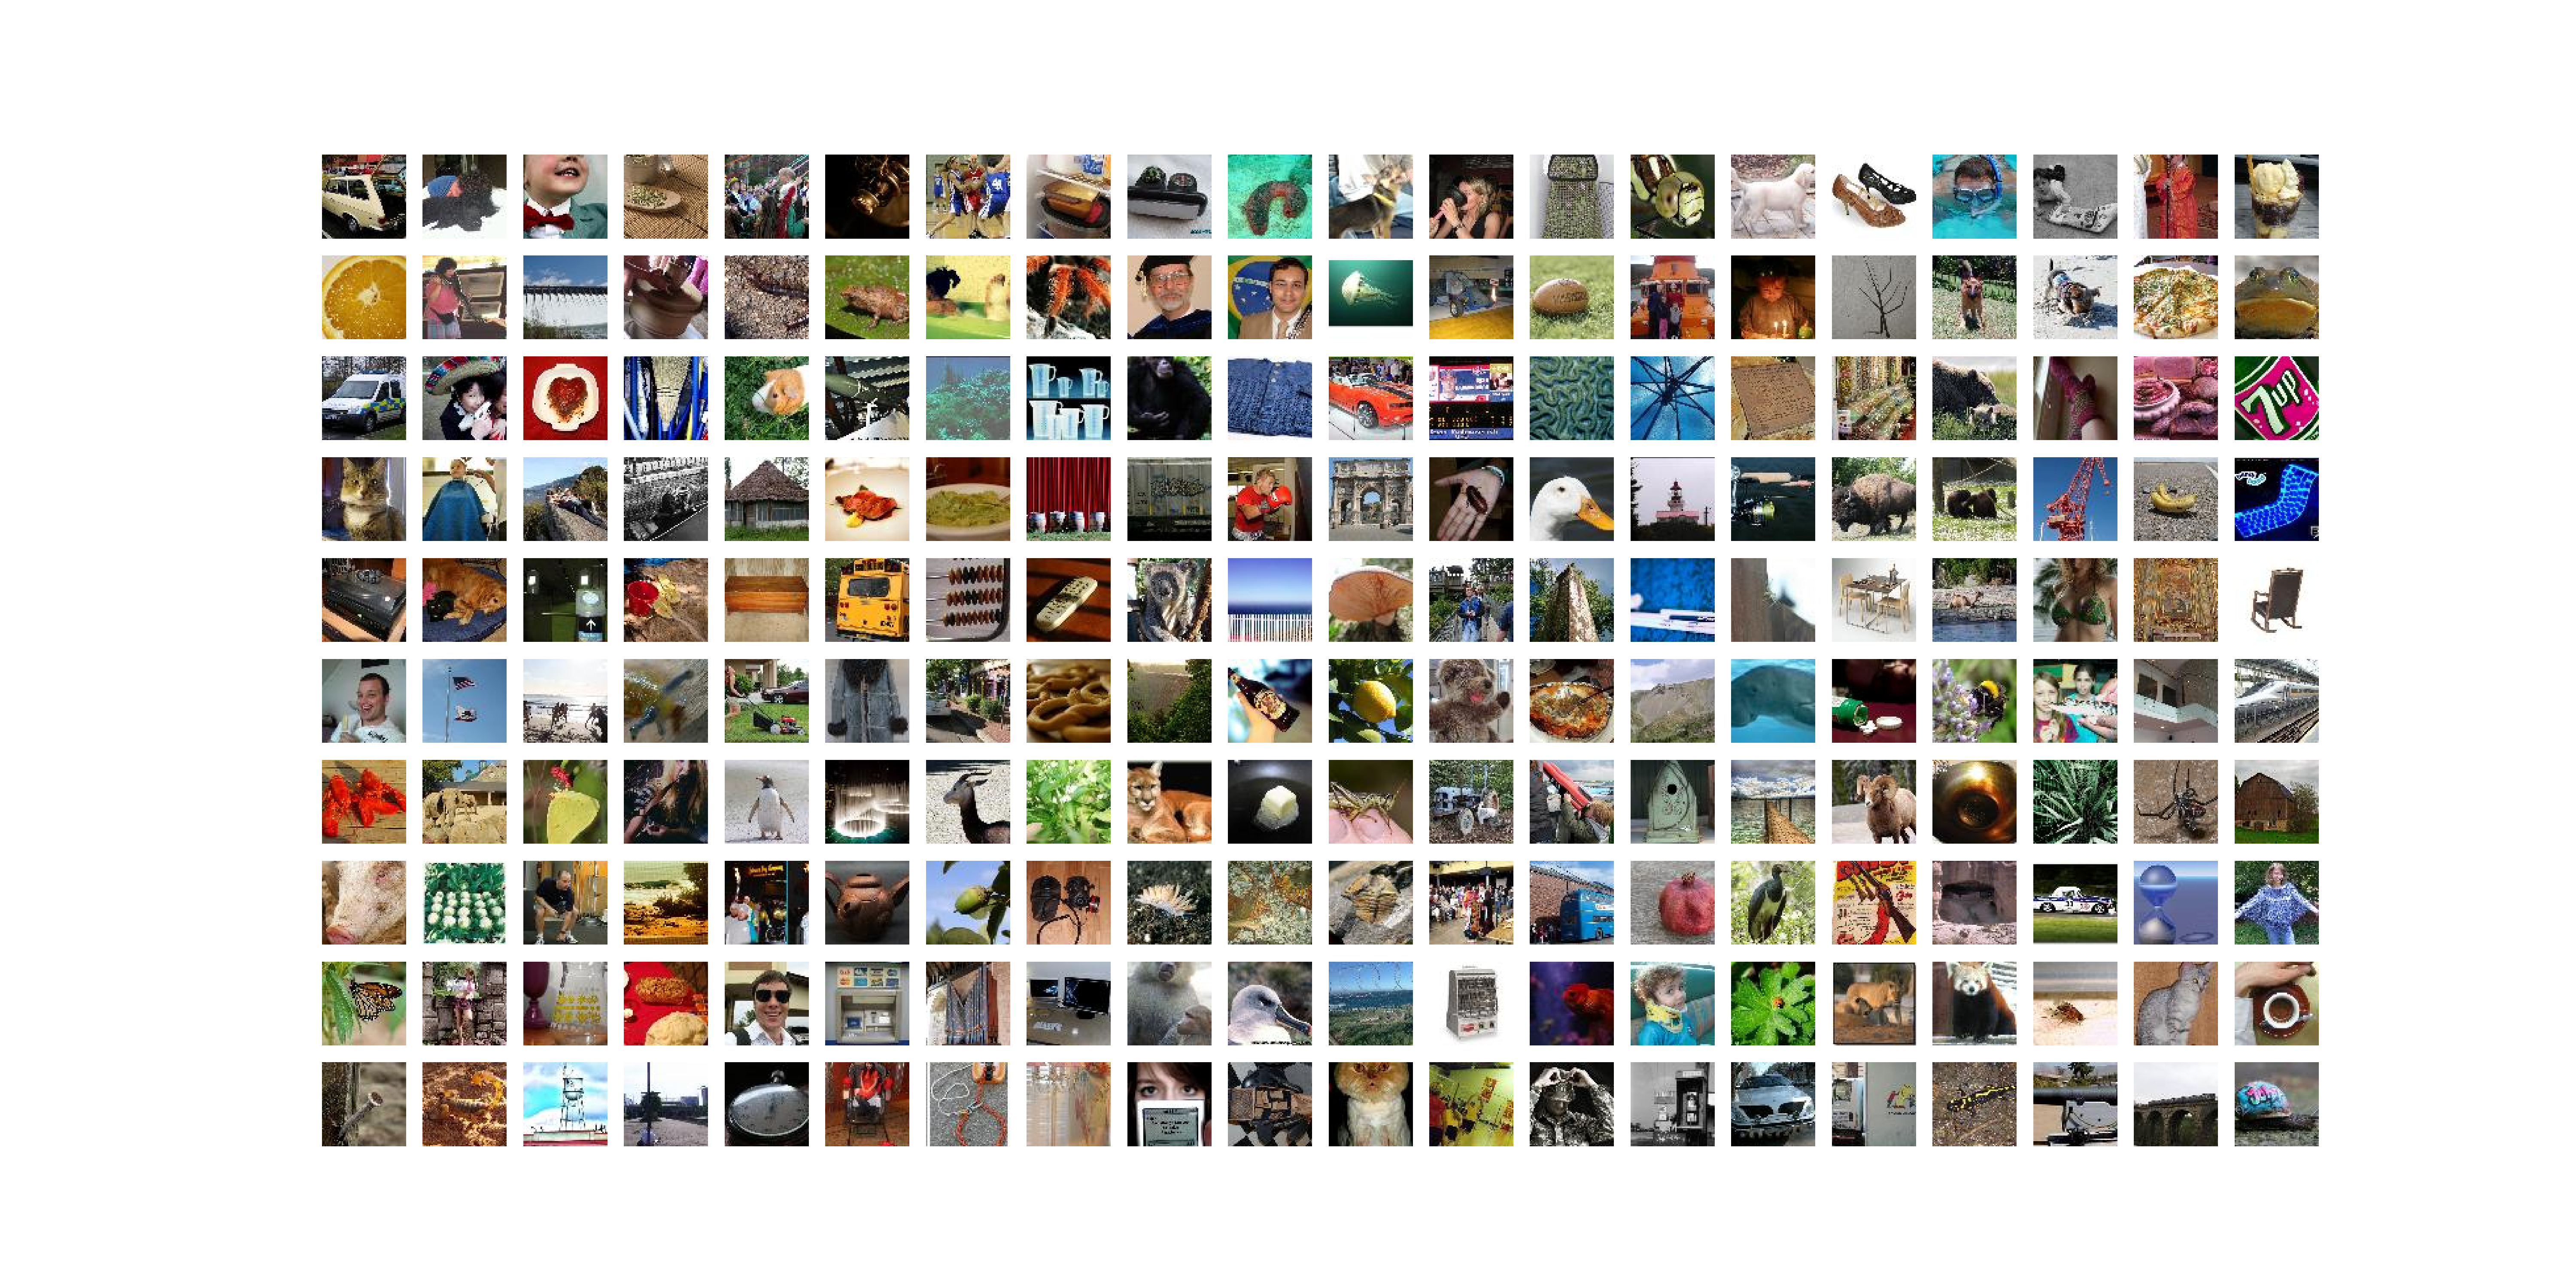
\includegraphics[width=0.7\textwidth]{chapter_dlo/assets/tinyimagenet_example.png}
  \caption{A sample grid of images from the Tiny ImageNet dataset. The images
    represent a subset of the 200 distinct classes, each image represents a
    unique class.}
  \label{fig:intro:tinyimagenet_examples}
\end{figure}

\subsection{Train, Validation and Test Sets}

In our experiments, for each dataset, we use 3 sets: train, validation and test
sets. The training set serves to train the model, while the validation set is
used to monitor the evolution of the performance metric on unseen data
throughout the training. The validation metric provides the necessary triggers
for the early stopping policy (\emph{i.e.} interrupting the training prematurely
if the validation metrics do not change over a given number of iterations). The
test set, on the other hand, is used to evaluate the model's performance on
entirely new data and to report the final test accuracy. When utilizing datasets
like CIFAR-10 and CIFAR-100, only training and testing sets are available. For
these datasets, we split the given train set in half with the following
proportions: 90\% of the original training set is used for training for the
network and the remaining 10\% is used as the validation set. On the other hand,
the TinyImageNet dataset does provide training, validation, and testing sets,
but the test set lacks annotations. Hence, we use 90\% of the training set for
model training and the remaining 10\% for validation. Instead of the unannotated
test set, we repurpose the original validation set to serve as the test set.
This is a common strategy employed by other implementations
\cite{hanyuanxu2018tinyimagenet,nbdt,alvinwan2020nbdt}.\\

\chapter{Deep Neural Network Compression}
\label{chap:sota}


\localtableofcontents

\section{introduction}
% TODO: dire que l'on va faire un petite overview des réseaux de neurones
% TODO: relier avec ce que l'on a dit avant (context netatmo)

% region: intro
The development of neural networks and the enhancement of their performances has
been accompanied by a significant growth of their size, particularly in the
number of weights constituting them. In parallel, the evolution of these
networks has given rise to various applications, particularly embedded ones,
whose resources are highly constrained in terms of computing power, energy
consumption or memory footprint. Alongside the increase in the size of these
networks, compression techniques have been devised, in order to enable the use
of these algorithms in the said applications.

% TODO: adapter la suite à ce qui a été fait.

This chapter focuses on these
techniques and presents state-of-the-art neural network compression methods,
predominantly based on reducing the number of weights. First, we will explore
ad-hoc architectures, referred to here as \emph{Efficient Architectures}. These
networks are lightweight networks that revolve around a core technique to reduce
their size while preserving performance as much as possible. Following this, we
will discuss \ac{NAS}, a method that automates the discovery of optimal network
architectures tailored to specific tasks or constraints, potentially leading to
more compact and efficient designs. Thereafter, we will examine fast convolution
techniques, which aim to accelerate the computation of convolutions in neural
networks, thereby reducing both the runtime and computational resources
required. Subsequently, we will delve into \ac{KD}, a process by which the
knowledge of a larger, more complex network (denoted the \emph{teacher}) is
transferred to a smaller, more efficient network (denoted the \emph{student}),
enabling the latter to achieve comparable performance with a reduced footprint.
Afterwards, we will address weight operations techniques, including methods such
as low-rank factorisation and other linear algebra techniques, which aim to
reduce the complexity and size of the networks by capitalising on inherent
redundancies and structures in the weight matrices. Lastly, we will consider
Neural Network Pruning, a set of techniques that involve the removal of
redundant or insignificant connections and weights from the network, resulting
in a sparser and more computationally efficient model.\\

% TODO: reorganiser le paragraphe précédent qui introduit les sections dont on
% va parler. Il faut être sûr que ça correspond aux sections qui suivent.

% endregion: intro

\section{Deep Learning overview}

Deep learning is a subfield of machine learning that focuses on the study of
\acp{DNN}. \acp{DNN} are a family of machine learning algorithms that have their
roots in \acp{ANN} that aim to learn a data representation from unstructured
data such as raw images, text or audio, in and end-to-end fashion. \acp{ANN}
were initially conceptualised based on the understanding of biological neural
networks present in the brain \cite{mcculloch1943logical,hebb2005organization}.
\citeauthor{rosenblatt1958perceptron} proposed in
\cite{rosenblatt1958perceptron} a theoretical model of a neuron, denoted the
\emph{perceptron}, which was capable of learning a linear decision boundary. The
perceptron model was later extended to multiple layers of neurons, giving rise
the \ac{MLP} \cite{rosenblatt1961principles,rumelhart1986learning}. A \acl{MLP}
is a type of artificial neural network that extends the concept of a
single-layer perceptron by including one or more hidden layers of neurons, with
each layer fully connected to the next, allowing the model to learn and
represent more complex, non-linear relationships in the input data. The term
\emph{deep} in the context of \acp{DNN} refers to the staking of multiple and
numerous layers within a neural network. A \ac{DNN} consist of layers, each
layer is an operation that takes information from the previous layers, process
it and then passes it through an activation function
\cite{glorot2011deep,DBLP:journals/pieee/LeCunBBH98,klambauer2017self} that
introduce non linearity, and finally this output is send to the next layer.
Among the most fundamental types of these layers are \emph{Convolutional} and
\emph{Dense} (or fully connected) layers. \\

\begin{figure}
    \centering
    \subfloat[Convolutional Layer\label{fig:sota:conv_layer}]{
        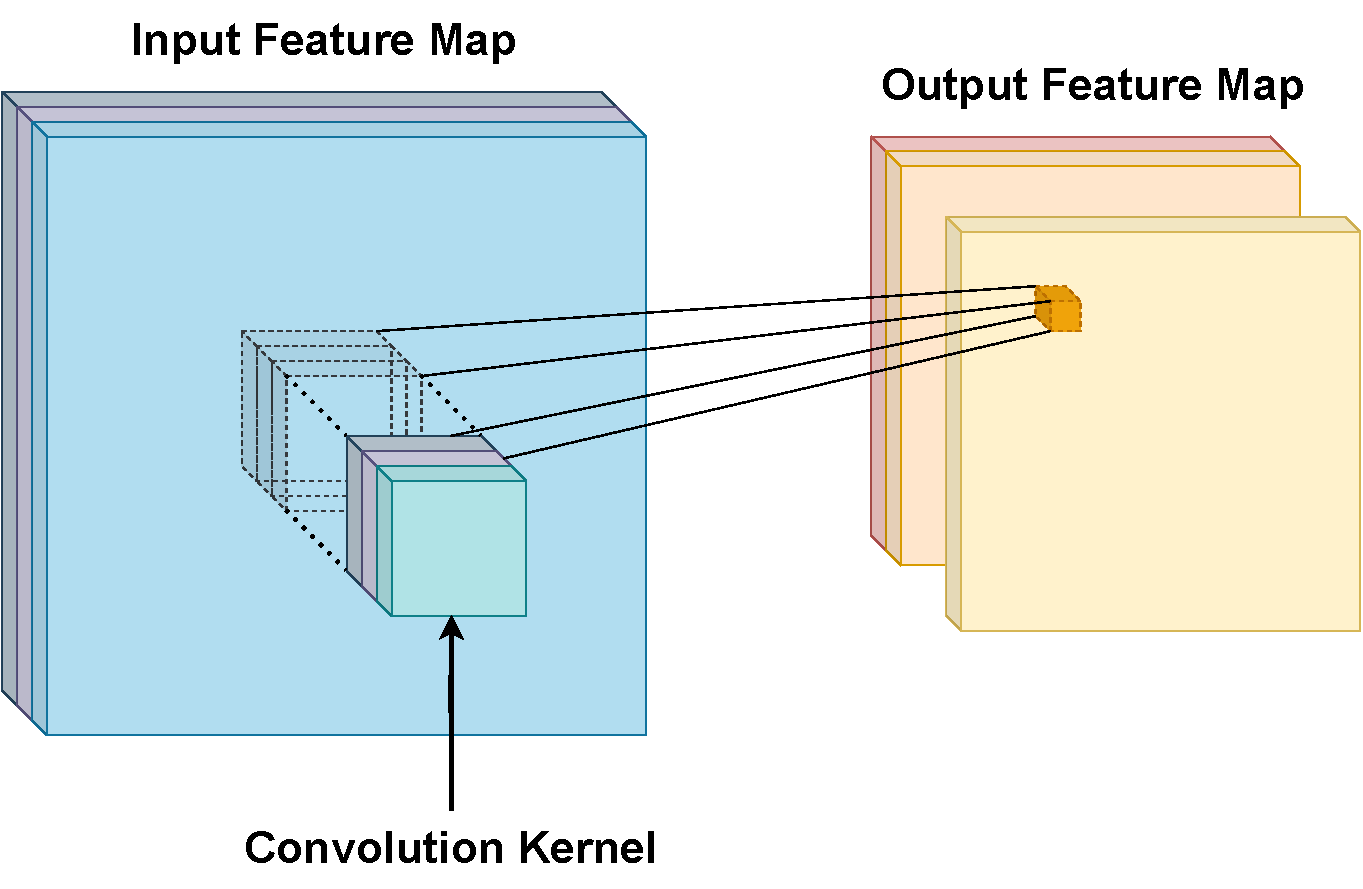
\includegraphics[width=0.49\textwidth]{chapter_sota/assets/conv_layer.pdf}}
        \subfloat[Dense Layer\label{fig:sota:dense_layer}]{
        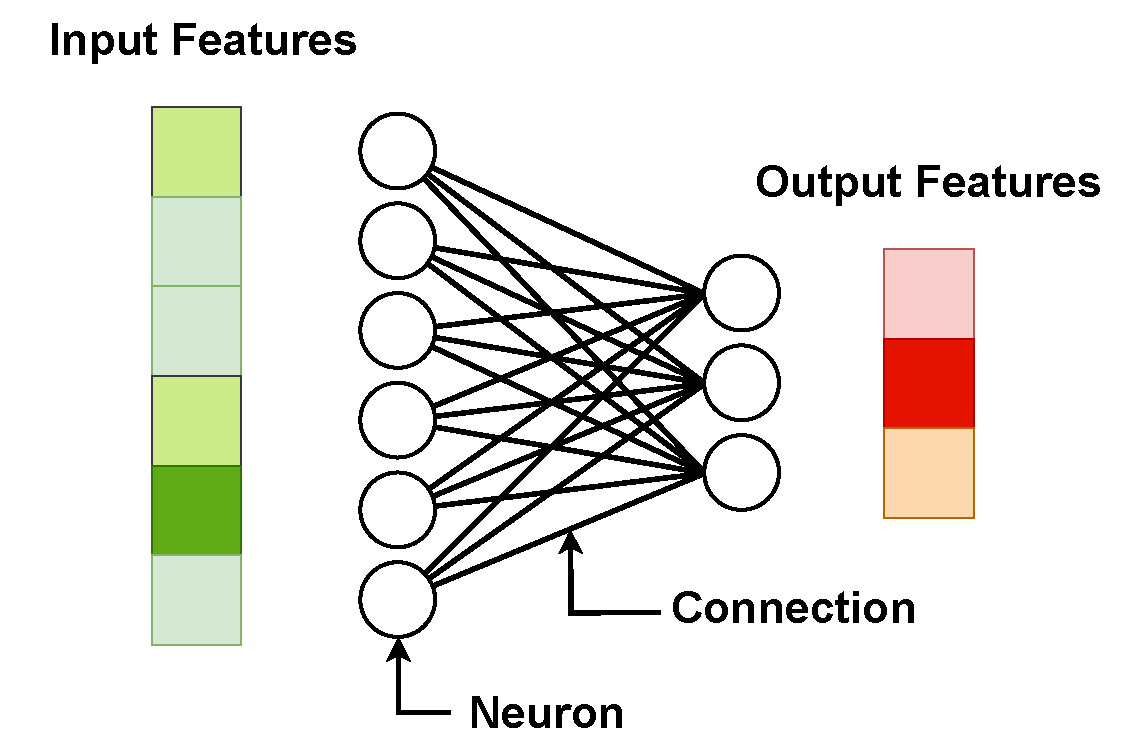
\includegraphics[width=0.49\textwidth]{chapter_sota/assets/dense_layer.pdf}}
        \caption{Conceptual representation of a convolutional layer and a dense
        layer. The convolutional layer (\cref{fig:sota:conv_layer}) takes a
        multi-channel input and produces a multi-channel output. Each coefficient of
        the output is computed by applying a convolution operation at a
        corresponding location in the input. The dense layer
        (\cref{fig:sota:dense_layer}) takes a vector input and produces a vector
        output. Each connection is represented by a weight in the weight matrix.}
    \label{fig:sota:layers}
    \end{figure}


Dense layers, often referred to as fully connected layers, are characterised by
neurons that connect to every neuron in the preceding layer. This characteristic
is central to \ac{MLP} networks, where these dense layers are stacked together.
Convolutional layers are typically used for image analysis tasks
\cite{DBLP:journals/pieee/LeCunBBH98}. They are composed of several kernels that
are convoluted with the input data. They are used for detecting edges, textures,
and patterns, and are often used as feature extractor. Typical neural network
targeted towards image processing are composed convolutional layers and thus
named \aclp{CNN}. In a such architecture, convolutional layers are stacked and
their output are usually fed into a fully-connected layer for further processing
\cite{DBLP:journals/corr/SimonyanZ14a,DBLP:conf/cvpr/HeZRS16,huang2017densely}.
Conceptual representations of these layers are shown in \cref{fig:sota:layers}
and a typical \ac{CNN} architecture is shown in \cref{fig:sota:lenet5,fig:sota:vgg16}.\\

\begin{figure}[htbp]
    \centering
    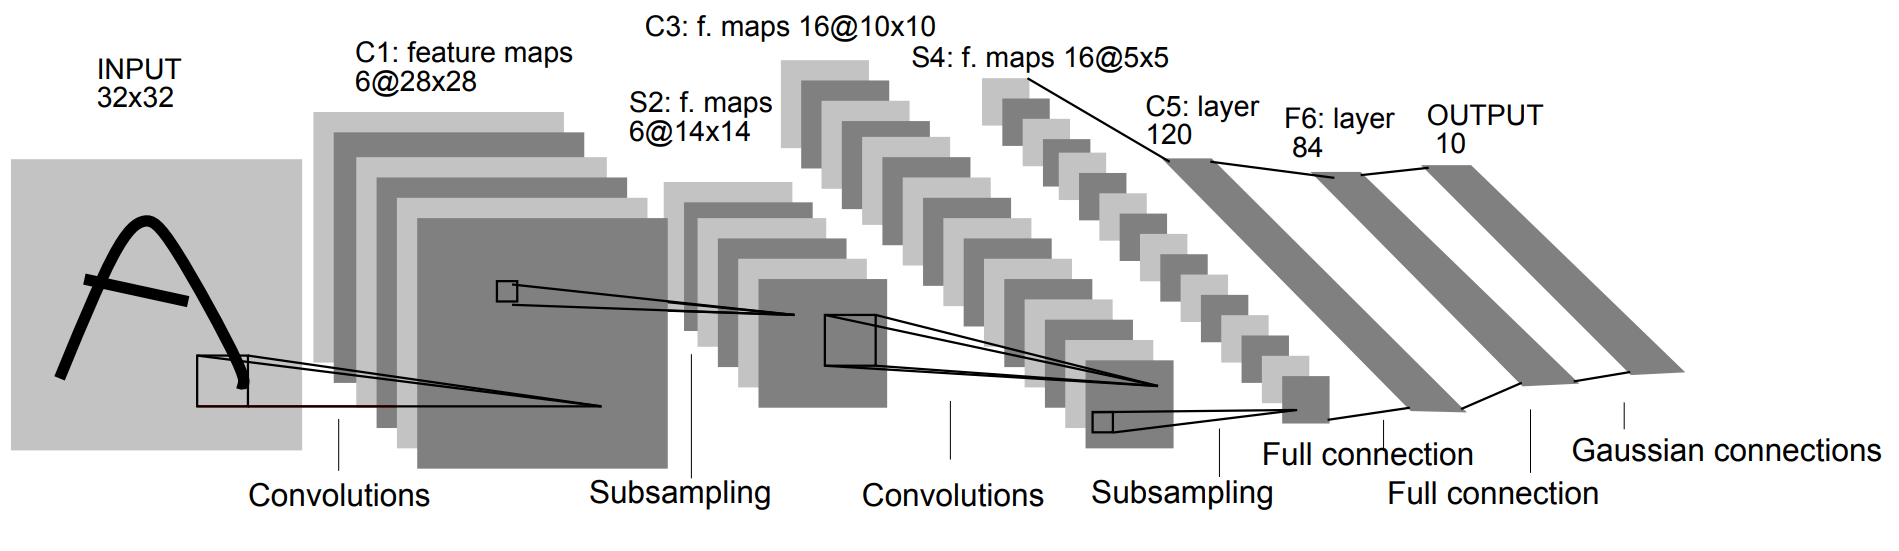
\includegraphics[width=0.70\textwidth]{chapter_sota/assets/lenet.png}
    \caption{Architecture of LeNet-5, a \acl{CNN} used for handwritten digit
    recognition. Image taken from \cite{DBLP:journals/pieee/LeCunBBH98}}
    \label{fig:sota:lenet5}
\end{figure}

\begin{figure}[htbp]
    \centering
    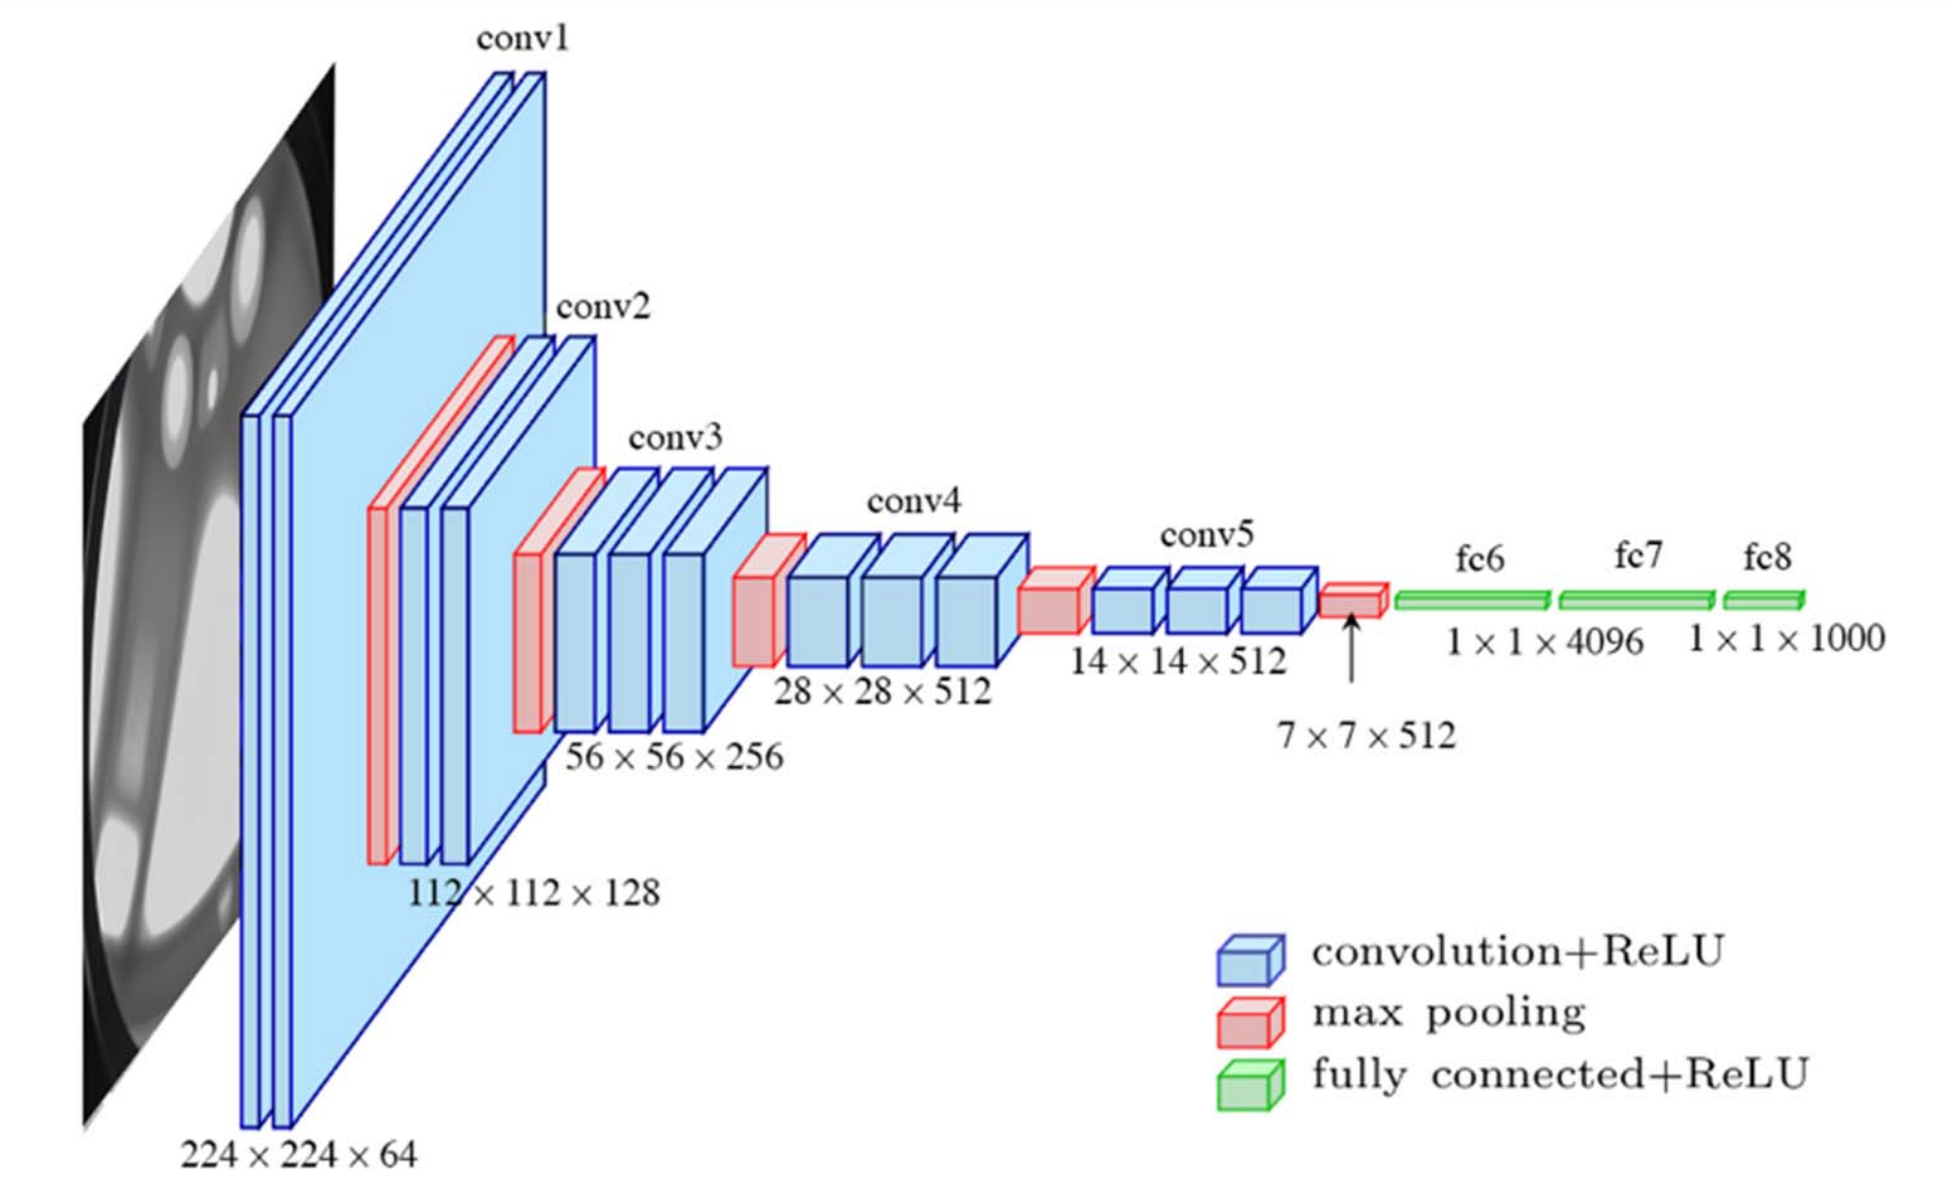
\includegraphics[width=0.7\textwidth]{chapter_sota/assets/vgg16.png}
    \caption{Architecture of the VGG16 network introduced in
    \cite{DBLP:journals/corr/SimonyanZ14a}. Image taken from
    \cite{ferguson2017automatic}}
    \label{fig:sota:vgg16}
\end{figure}


The process of training a neural network involves adjusting the weights of the
network to minimize a loss function. The loss function is a measure of the error
between the predicted output of the network and the ground truth. Since neural
networks are differentiables, the weights can be adjusted using gradient-based
methods. The most common method is \acf{SGD}, derived from the Robbins–Monro
algorithm \cite{robbins1951stochastic}. In \ac{SGD}, the gradient of the loss
function is computed for a random subset of the data (a \emph{batch} or
\emph{mini-batch}), and the weights are shifted in the direction that decreases
the loss function. This direction is computed via the backpropagation algorithm
\cite{rumelhart1986learning} which calculates the gradient of the loss with
respect to each weight using the chain rule. \acl{SGD} is a prevalent method for
loss function optimisation in neural networks, however, numerous other methods also
exist. These include momentum-based strategies \cite{sutskever2013importance}, adaptive
learning rate approaches \cite{zeiler2012adadelta} and moment estimation
techniques \cite{kingma2014adam}.\\


\section{Neural Networks Size and Achitecture Evolution}

% TODO: ajouter les bonnes refs
% TODO: relecture
% TODO: ajouter un graph de l'évolution de la taille des réseaux

The evolution of neural networks is characterized by a consistent increase in
their size and performance, alongside the introduction of new architectural
modifications to address limitations of their predecessors (see
\cref{fig:sota:net_sizes}). In 1998, LeNet-5 was developed for digit recognition
\cite{DBLP:journals/pieee/LeCunBBH98}, constituting a relatively simple network
with seven layers. Its size was significantly small compared to the contemporary
models. With the introduction of AlexNet \cite{DBLP:conf/nips/KrizhevskySH12} in
2012, the network size considerably grew, comprising more layers and neurons to
handle more complex tasks like large-scale image recognition. AlexNet tackled
the overfitting issue in LeNet-5 with the use of data augmentation and dropout
techniques.\\


The next advancement was the VGG networks family
\cite{DBLP:journals/corr/SimonyanZ14a} %, introduced in 2014 
which emphasized the importance of depth in neural networks. With up to 19
layers, VGG expanded on AlexNet's deep architecture, but the increased depth led
to vanishing gradient problems. In the same year, Google's Inception (or
GoogLeNet) \cite{DBLP:conf/cvpr/SzegedyLJSRAEVR15} was introduced, addressing
this issue with its novel inception modules, which allowed the network to learn
at varying scales and increased computational efficiency, without overly
increasing the network size.\\

%In 2015, 
Later, the ResNet models family was proposed in \cite{DBLP:conf/cvpr/HeZRS16},
which effectively tackled the vanishing gradient problem by introducing skip (or
shortcut) connections, allowing gradients to backpropagate directly through
several layers. These shortcut connections also allowed the network to grow in
depth up to 152 layers without a significant increase in computational cost.
However, a challenge remained with the constant need for careful design to
manage feature-map sizes.\\

In response, DenseNet was proposed.% in 2017, 
It connects each layer to every other layer in a feed-forward fashion. By
reinforcing the propagation of features and gradients through the network,
DenseNet alleviated the vanishing-gradient problem and further improved upon the
network's ability to pass on information from earlier layers to later ones.
Thus, through these chronological advancements, neural networks not only grew in
size but also improved in performance, becoming more efficient and capable of
handling more complex tasks.

\begin{figure}[htbp]
    \centering
    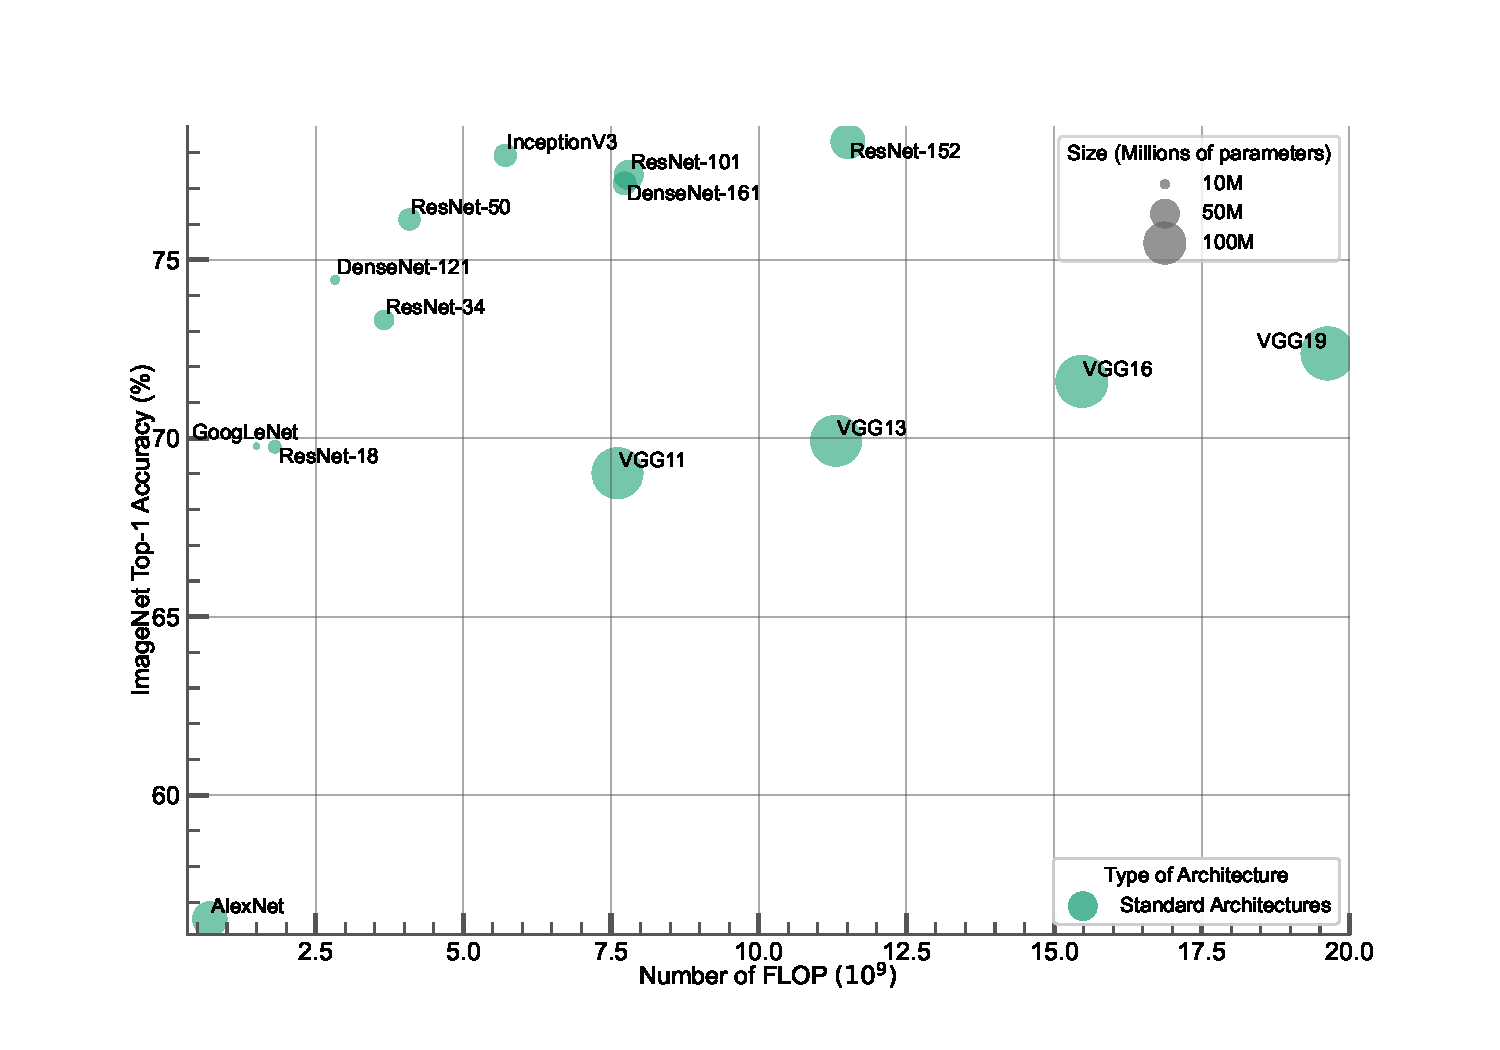
\includegraphics[width=0.7\textwidth]{chapter_sota/assets/network_sizes_normal.pdf}
    \caption{Networks size comparison. The \emph{x-axis} represents the number
    of \acp{FLOP} required to process a single image. The \emph{y-axis}
    represents the Top-1 accuracy on the ImageNet \cite{deng2009imagenet}
    dataset, and the size of the circles represents the number of parameters in
    the network. Numbers are taken from \cite{pytorch_vision}}
    \label{fig:sota:net_sizes}
\end{figure}

\section{Fast convolutions}
\label{sec:sota:fast_convolutions}


Neural networks, utilise two fundamental mathematical operations: convolution
and matrix multiplication. However, performing these operations can be
computationally demanding, particularly with large and complexe networks. This
can lead to significant processing times, posing a challenge for real-time or
resource-limited applications. To mitigate this, some research efforts have been
focused on developing techniques to speed up these operations. These strategies
range from optimizing the underlying algorithms to leveraging hardware
acceleration, with the objective of enhancing the speed and efficiency of neural
network computations.\\


The most popularalgorithm accelerating convolution operations rely on the
\ac{FFT}
\cite{DBLP:conf/nips/ChiJM20,DBLP:journals/npl/LinY19,DBLP:conf/pkdd/PrattWCZ17},
and leverage the Convolution Theorem. The Convolution Theorem states that the
convolution of two signals in the source domain is the product of the two
signals in the Fourier domain. This allows for a faster computation of the 2D
convolution by using the \ac{FFT} to compute the convolution in the frequency
domain \cite{oppenheim1997signals}.\\


Other algorithms focus on optimising matrix operations, such as the Strassen
algorithm \cite{strassen1969gaussian}, used in \cite{DBLP:conf/icann/CongX14}.
It is a fast method for matrix multiplication that reduces the computational
complexity from the standard $\mathcal{O}(n^{3})$ to approximately
$\mathcal{O}(n^{2.807})$ by recursively dividing the matrices of size $n$ into 4
submatrices of size $\frac{n}{2} \times \frac{n}{2}$, reorganising and combining
these multiplications to perform only 7 instead of 8 matrix multiplications. The
Strassen algorithm has later been refined by \citeauthor{coppersmith1987matrix},
who introduced the Coppersmith-Winograd algorithm \cite{coppersmith1987matrix}.
The latter brings down the complexity to $\mathcal{O}(n^{2.376})$. This
algorithm is used in various works, mostly targeted towards a specific \ac{FPGA}
architecture \cite{liu2018efficient,lu2018spwa,wang2020winonn}.\\


Another technique for optimising convolutions is the use of Toeplitz matrices. A
Toeplitz matrix, or diagonal-constant matrix, has the unique characteristic of
each descending diagonal from left to right being constant. $T$ is an example of
a Toeplitz matrix. This property is particularly useful for convolutions, as
they can be expressed as a multiplication by a Toeplitz matrix
\cite{gray2006toeplitz}. This algorithm has been used in
\cite{liao2019compressing}, with a focus on \ac{FPGA} architectures. Note that
the representation of a convolution as a product with a Toeplitz matrix can
further be accelerated by using the aforementioned optimisations to the matrix
multiplication algorithm.\\

$$
T = 
\left(
\begin{array}{cccc}
a & b & c & d \\
e & a & b & c \\
f & e & a & b \\
g & f & e & a \\
\end{array}
\right)
$$

The algorithms presented in this section offer significant acceleration in the
computation of convolution operations. However, their optimal efficiency is
bound to the use of relatively large matrices. Current architectures
\cite{DBLP:conf/cvpr/HeZRS16, huang2017densely, liu2018efficient} predominantly
use small $3 \times 3$ kernels, rendering the direct application of these
acceleration techniques less beneficial. As a consequence, these techniques have
not gained widespread adoption in contemporary deep learning architectures.



% TODO: Paragraphe sur l'entrainement Stochastique

% TODO: Paragraghe pour expliquer que l'on peut accélérer 




\section{Teaching Paradigm}


\acf{KD} is a method that aims to transfer the knowledge of a large, complex and
accurate network referred to as the \emph{teacher} to a smaller, more efficient
one called the \emph{student}. The student is trained with a combination of the
main task loss as well as a supplementary supervision signal which is derived
from the feature maps of the teacher network at various depths.\\

Methods in this paradigm are mostly based on the seminal work of
\citeauthor{DBLP:journals/corr/HintonVD15} \cite{DBLP:journals/corr/HintonVD15}.
The latter seeks to train simple networks with \acl{KD} yielding better
performances compared to those trained from scratch. \ac{KD} relies on teacher
and student networks, where the logits of the former are used as an additional
supervision signal for the latter. When trained separately, the student network
can only rely on classification labels in order to learn its own data
representation while \ac{KD} relies on the logits of the teacher network which
provide more insight about the hidden representations.\\

Inspired by \ac{KD}, \cite{DBLP:journals/corr/RomeroBKCGB14} introduced FitNet,
a two-stage training algorithm, where an intermediate layer of the teacher is
chosen as a \emph{hint}\footnote{\emph{Hint} is the terminology used by
\citeauthor{DBLP:journals/corr/RomeroBKCGB14}
\cite{DBLP:journals/corr/RomeroBKCGB14} to denote a feature map used as a target
for the student network.} for an intermediate layer of the student. First, the
student is trained up to its selected layer to mimic the hint feature map. Then,
the whole student network is trained with standard \ac{KD} against the whole
teacher. In the first step, a regressor is needed in order to adapt the
dimensions of the feature map, which may differ from the teacher to the student
networks, as illustrated in \cref{fig:sota:kd_frameworks}.
\citeauthor{DBLP:conf/cvpr/YimJBK17} argue that the direct feature map matching
utilised by FitNets is overly restrictive. Drawing inspiration from the
techniques used in \cite{DBLP:journals/corr/GatysEB15a} for style transfer, they
propose an alternative method. In the context of style transfer, the Gram matrix
of the feature maps is employed to encapsulate the texture information of an
image. Adapting this approach, the method presented in
\cite{DBLP:conf/cvpr/YimJBK17} calculates the Gram matrix across multiple layers
feature maps. This computed Gram matrix, dubbed the Flow of Solution Procedure
(FSP) matrix, then serves as a \emph{hint} for the student network, guiding its
training process.\\

\begin{figure}[htbp]
    \centering
    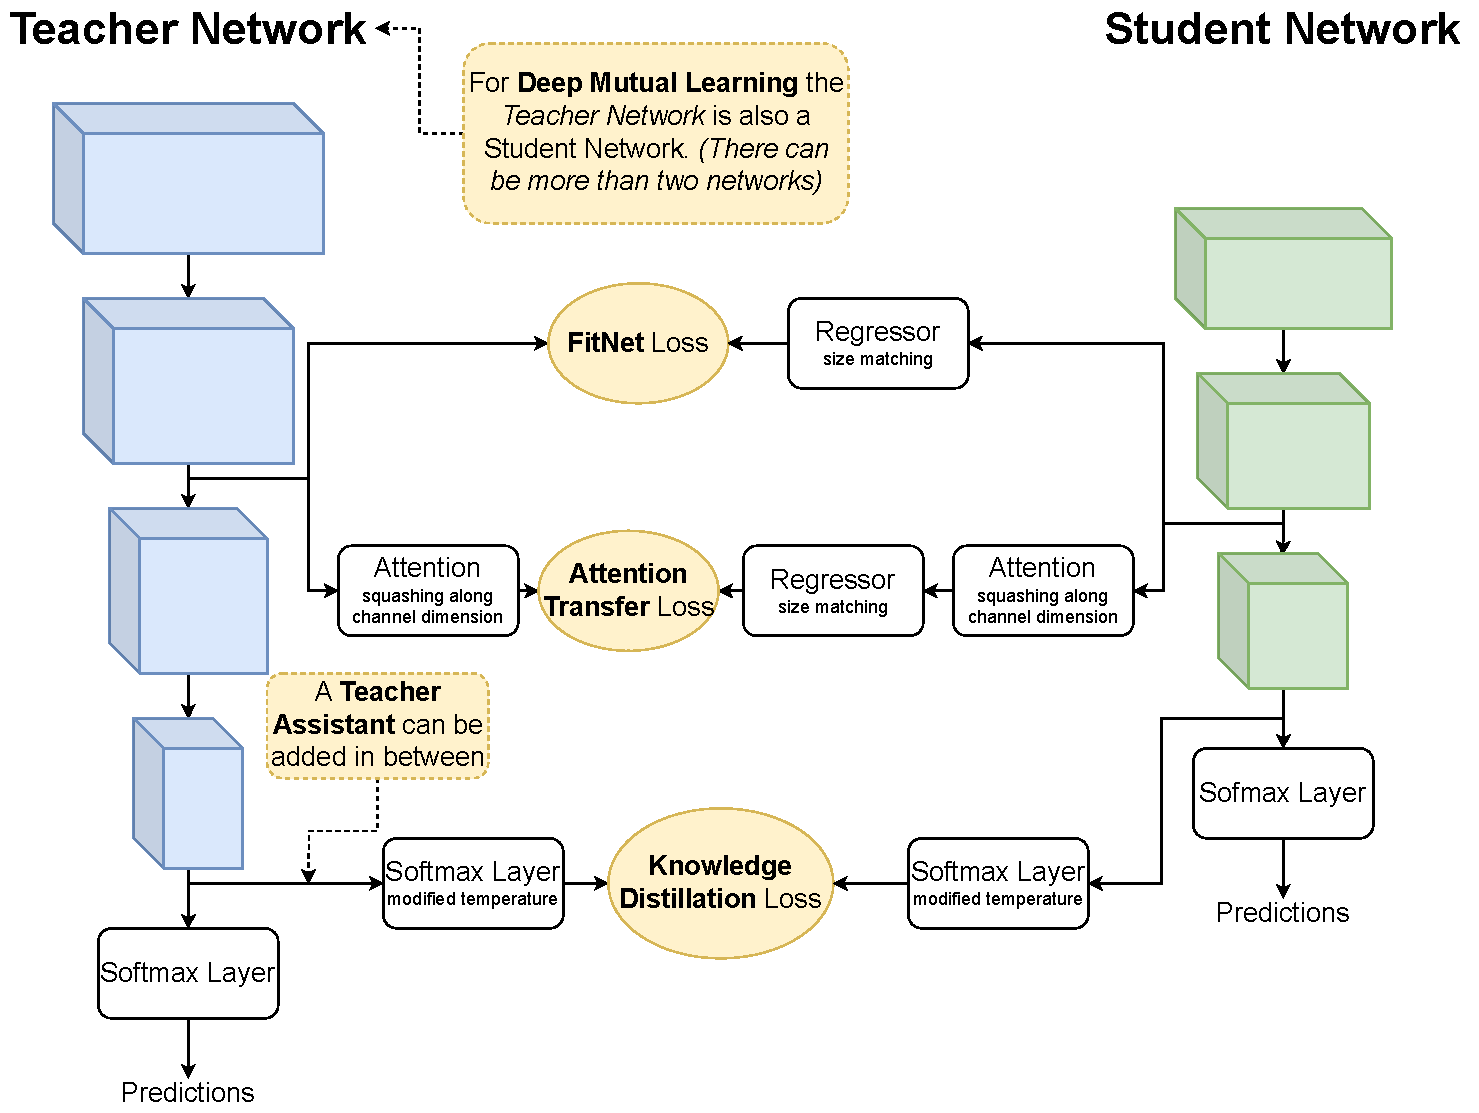
\includegraphics[width=0.75\textwidth]{chapter_sota/assets/kd_frameworks.pdf}
    \caption{Overview of various knowledge distillation frameworks. From top to
    bottom, left to right: Deep Mutual Learning
    \cite{DBLP:conf/cvpr/ZhangXHL18}, FitNet
    \cite{DBLP:journals/corr/RomeroBKCGB14}, Attention Transfer
    \cite{DBLP:conf/iclr/ZagoruykoK17}, Teacher Assistant
    \cite{DBLP:conf/aaai/MirzadehFLLMG20} and Knowledge Distillation
    \cite{DBLP:journals/corr/HintonVD15}.}
    \label{fig:sota:kd_frameworks}
\end{figure}

In practice, handling full-dimensional feature maps is cumbersome. That is why,
in order to avoid this issue, \cite{DBLP:conf/iclr/ZagoruykoK17} use an
attention map generated by squashing the feature maps to a 2D map allowing for a
smaller 2D regressor to match attention map dimensions. Note that the
aforementioned knowledge transfer methods require teacher-student pairs and
assume that teachers are large trained models. \cite{DBLP:conf/cvpr/ZhangXHL18}
relax this assumption by proposing Deep Mutual Learning, which enables a pool
of networks of different architectures to learn together, provided that they
have the same logit dimensions, and none of the models in the pool requires a
pretraining step. The uncertainty of each model is distilled to each other,
which creates additional knowledge.\\

In all the aforementioned methodos, the efficacy of knowledge distillation, and
consequently, the final performance of the student network, is significantly
influenced by the disparity in size between the student and teacher networks.
When this size discrepancy is excessive, the student network may encounter
difficulties in adequately aligning with the teacher logits, thus preventing
optimal knowledge distillation. In order to tackle this issue,
\citeauthor{DBLP:conf/aaai/MirzadehFLLMG20} introduced the concept of
\emph{Teacher Assistant}: networks of intermediary dimensions that aim at
bridging the gap between student and teacher
\cite{DBLP:conf/aaai/MirzadehFLLMG20}. Knowledge is first distilled from the
teacher to the teacher assistant, and then from the teacher assistant to the
student, resulting in improved performances compared to straightforward \ac{KD}.\\

\begin{figure}[htbp]
    \centering
    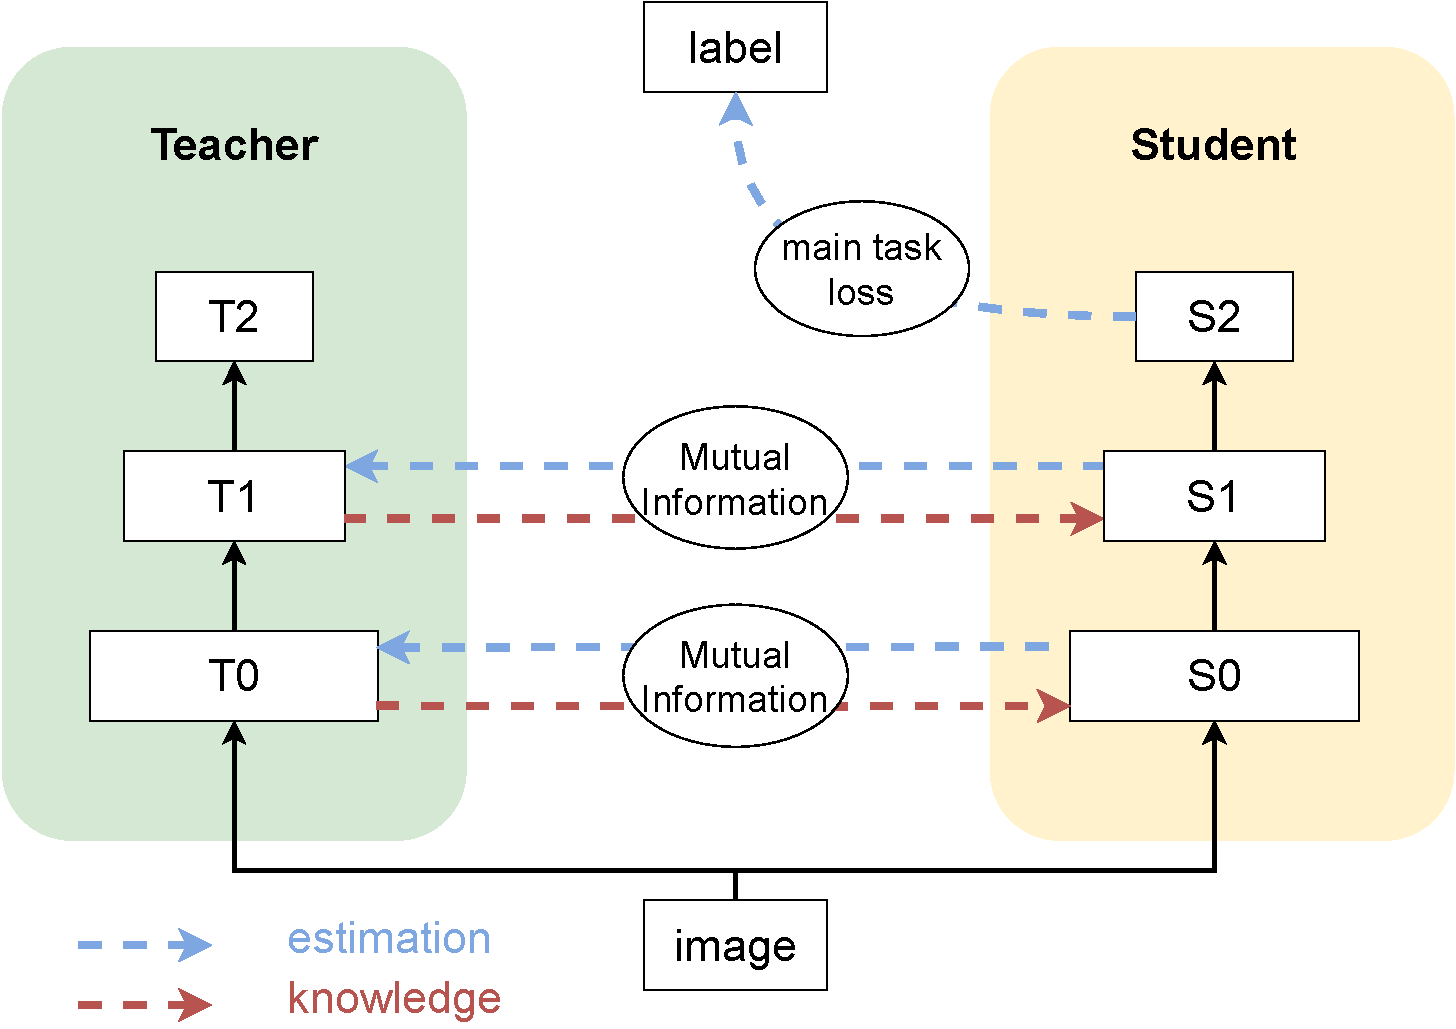
\includegraphics[width=0.7\textwidth]{chapter_sota/assets/variational_info_distillation.pdf}
    \caption{Conceptual scheme of \cite{DBLP:conf/cvpr/AhnHDLD19}. The student
    network efficiently learns the main task while retaining high mutual information
    with the teacher network. The mutual information is maximised by learning to
    estimate the distribution of the activations in the teacher network, provoking
    the transfer of knowledge. Adapted from the original
    scheme found in \cite{DBLP:conf/cvpr/AhnHDLD19}}
    \label{fig:sota:vid_scheme}
\end{figure}

Other approaches that do not rely on direct feature map or logit matching have
been proposed. \cite{DBLP:conf/cvpr/AhnHDLD19} introduced Variational
Information Distillation, which indirectly maximises the mutual information
between the student and the teacher. This is done by using \emph{variational
information maximisation} \cite{barber2004algorithm} to maximise a variational
lower bound of the mutual information, since directly maximising the latter is
intractable in practice (see \cref{fig:sota:vid_scheme}). Likewise,
\cite{DBLP:conf/eccv/PassalisT18} proposed a Probabilistic Knowledge Transfer
method that does not match logits or feature maps, but rather represents the
latter as a probability distribution and minimises divergence between the two
(see \cref{fig:sota:pkt_scheme}).\\


\begin{figure}[htbp]
    \centering
    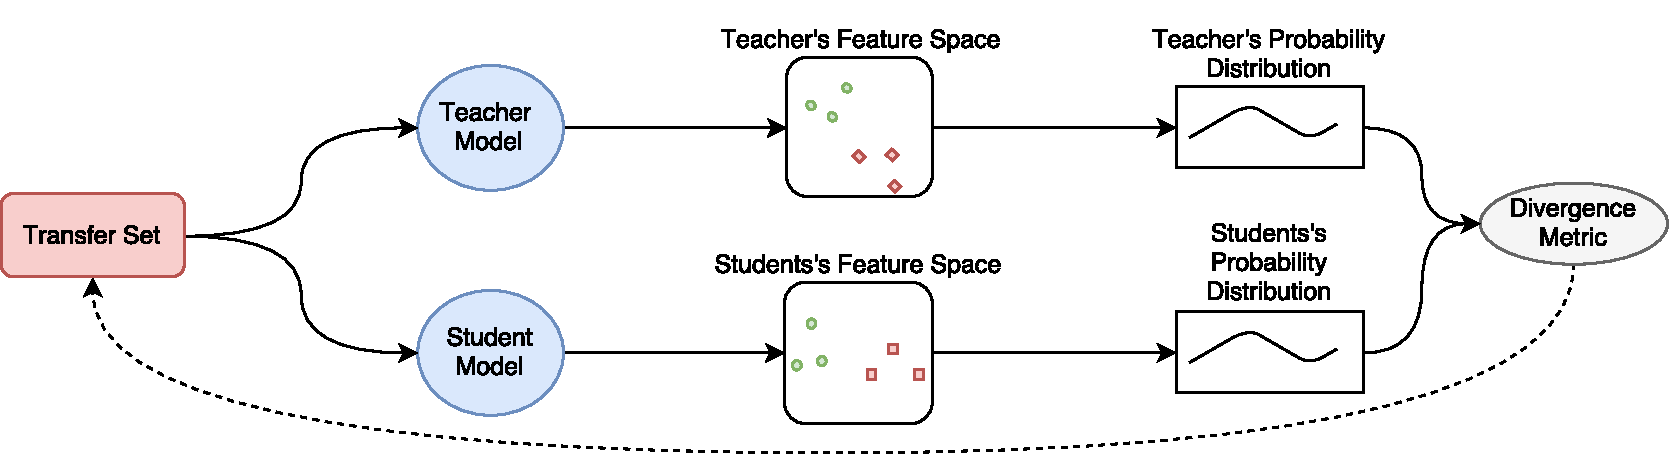
\includegraphics[width=0.7\textwidth]{chapter_sota/assets/pkt_diagram.pdf}
    \caption{Conceptual scheme of the
    Probabilistic Knowledge Transfer method. Both the student and the teacher
    feature maps are modelled using probability distributions. The divergence of the
    latter is minimised in order to transfer knowledge from the teacher to the
    student. Illustration taken from \cite{DBLP:conf/eccv/PassalisT18}.}
    \label{fig:sota:pkt_scheme}
\end{figure}

\section{Architecture Design}

\subsection{Building Blocks for Efficient Architecture Design}
\label{sec:sota:efficient_archi}
% region: depthwise separable convolutions

One of the initial strategies towards achieving efficiency in neural network
architectures is the use of depthwise separable convolutions. This technique,
utilised in \cite{howard2017mobilenets} and \cite{DBLP:conf/icml/TanL19},
separates the standard convolution operation into two distinct steps: a
depthwise convolution and a pointwise convolution (see
\cref{fig:sota:depthwise_conv_vs_standard_conv}). By decomposing the operations
in this manner, the computational complexity is markedly reduced while still
retaining the ability to capture spatial and channel-wise information. Consider
an input feature map with $C_\text{in}$ channels of arbitrary width and height
and $C_\text{out}$ convolution kernels of size $k\times k \times C_\text{in}$. A
standard convolution algorithm will need $C_\text{in} \times C_\text{out} \times
k \times k$ \ac{MAC} operations to produce a $1 \times 1 \times C_\text{out}$
element of the output feature map. In contrast, a depthwise separable
convolution algorithm will first apply a $k\times k \times 1$ convolution kernel
to the $C_\text{in}$ channels and then perform $C_\text{out}$ pointwise
convolutions with $1\times 1 \times C_\text{in}$ kernels to produce the same
$1\times 1 \times C_\text{out}$ element. This effectively reduces the number of
parameters to $C_\text{in} \times (C_\text{out} + k \times k)$, essentially
reducing the number of computations required to produce a $1 \times 1 \times
C_\text{out}$ element by a factor of\\

$$\displaystyle\frac{C_\text{out}\times k \times k}{C_\text{out} + k \times k}.$$\\

\begin{figure}[htbp]
\centering
\subfloat[Standard Convolution\label{fig:sota:standard_convolution}]{
    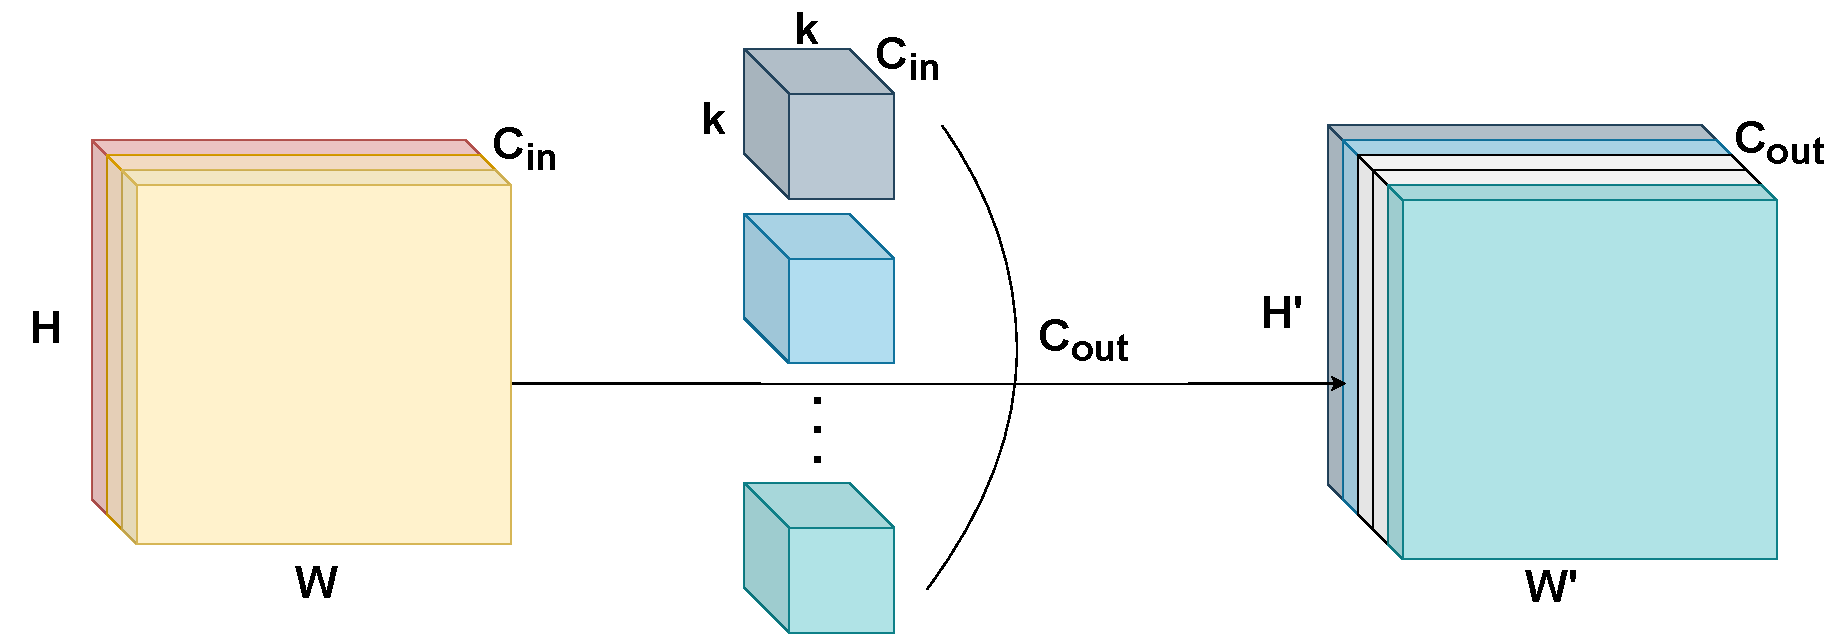
\includegraphics[width=0.70\textwidth]{chapter_sota/assets/standard_conv_scheme.pdf}}\\
    \vspace{1cm}
\subfloat[Depthwise Separable
    Convolution\label{fig:sota:depthwise_convolution}]{
    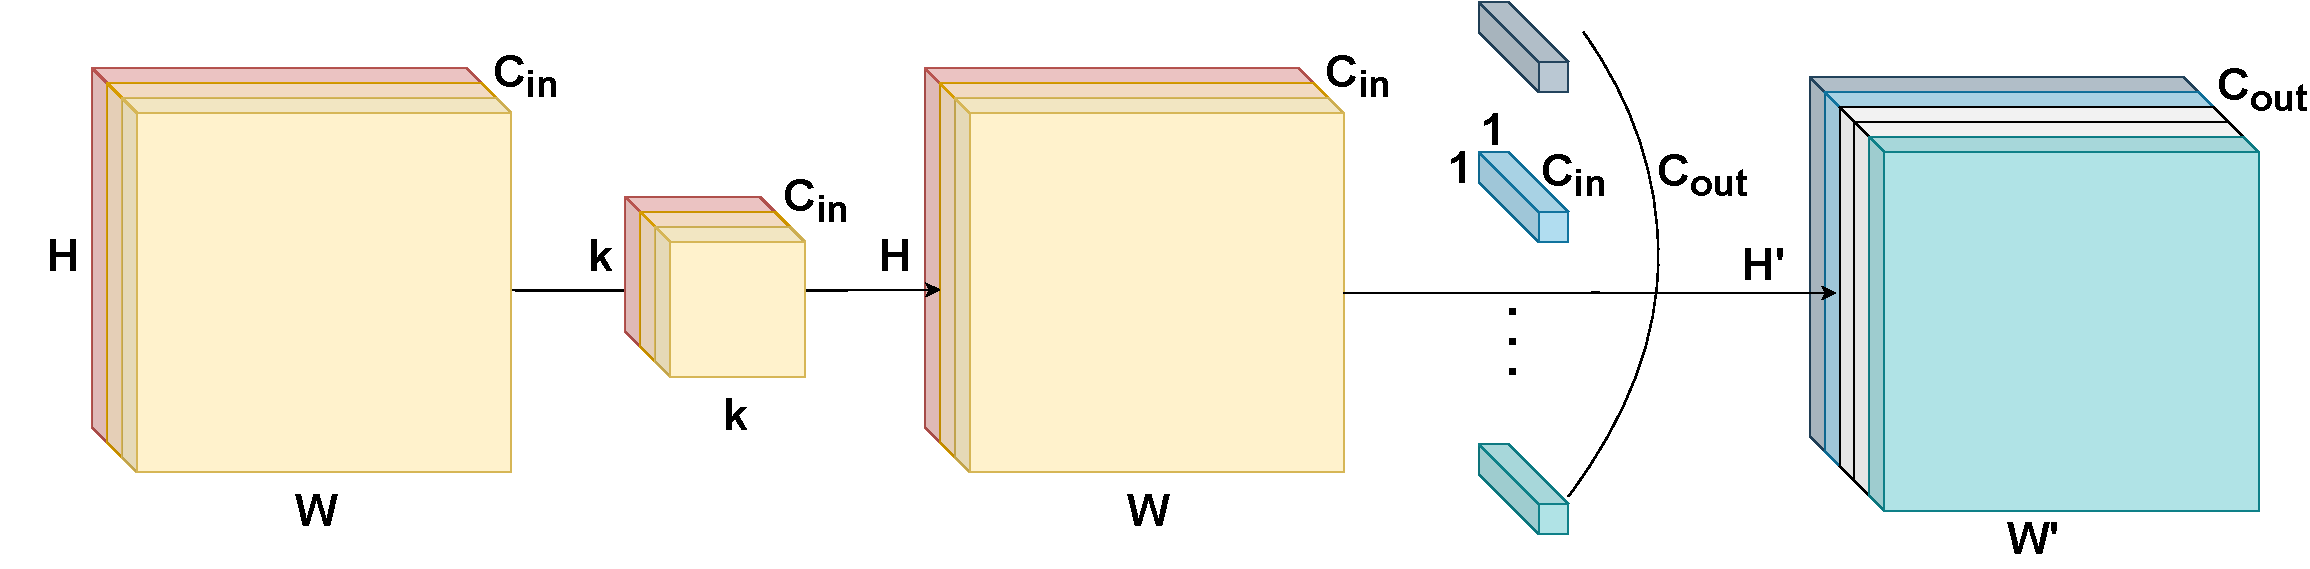
\includegraphics[width=0.70\textwidth]{chapter_sota/assets/depthwise_sep_conv_scheme.pdf}}
    \caption{Illustration schemes of the standard and depthwise separable
    convolution. The standard convolution uses $C_\text{out}$ kernels of size
    $k\times k \times C_\text{int}$. The depthwise separable convolution is
    split into two steps: \emph{(i)} a convolution with $C_\text{in}$ kernels
    of size $k \times k$ and \emph{(ii)} a convolution with $C_\text{out}$
    kernels of size $1\times 1 \times C_\text{int}$.
    Best viewed in colours.}
\label{fig:sota:depthwise_conv_vs_standard_conv}
\end{figure}

% endregion: depthwise separable convolutions

% region: fire module
An alternative approach for designing efficient architectures involves the
integration of \emph{fire modules}, as proposed in
\cite{DBLP:journals/corr/IandolaMAHDK16}. These modules aim to minimise
computational requirements by employing two distinct strategies: \emph{(i)}
diminishing the number of input channels supplied to the following conventional
$k\times k$ convolutions and \emph{(ii)} substituting a portion of the
resource-intensive $k\times k$ convolutions with pointwise convolutions, which
possess $k^2$ times fewer parameters. The initial strategy is applied within the
\emph{Squeeze Layer} of the \emph{fire module}, which functions to decrease the
number of input channels delivered to the \emph{Expand Layer}, subsequently
reducing the parameter count in the \emph{Expand Layer} kernels. The second
strategy is implemented in the \emph{Expand Layer}, where some $3\times3$
convolutions are replaced with $1\times1$ variants. Even though the $1\times1$
convolutions capture less spatial information, they are significantly less
computationally demanding.\\

\begin{figure}[htbp]
    \centering
    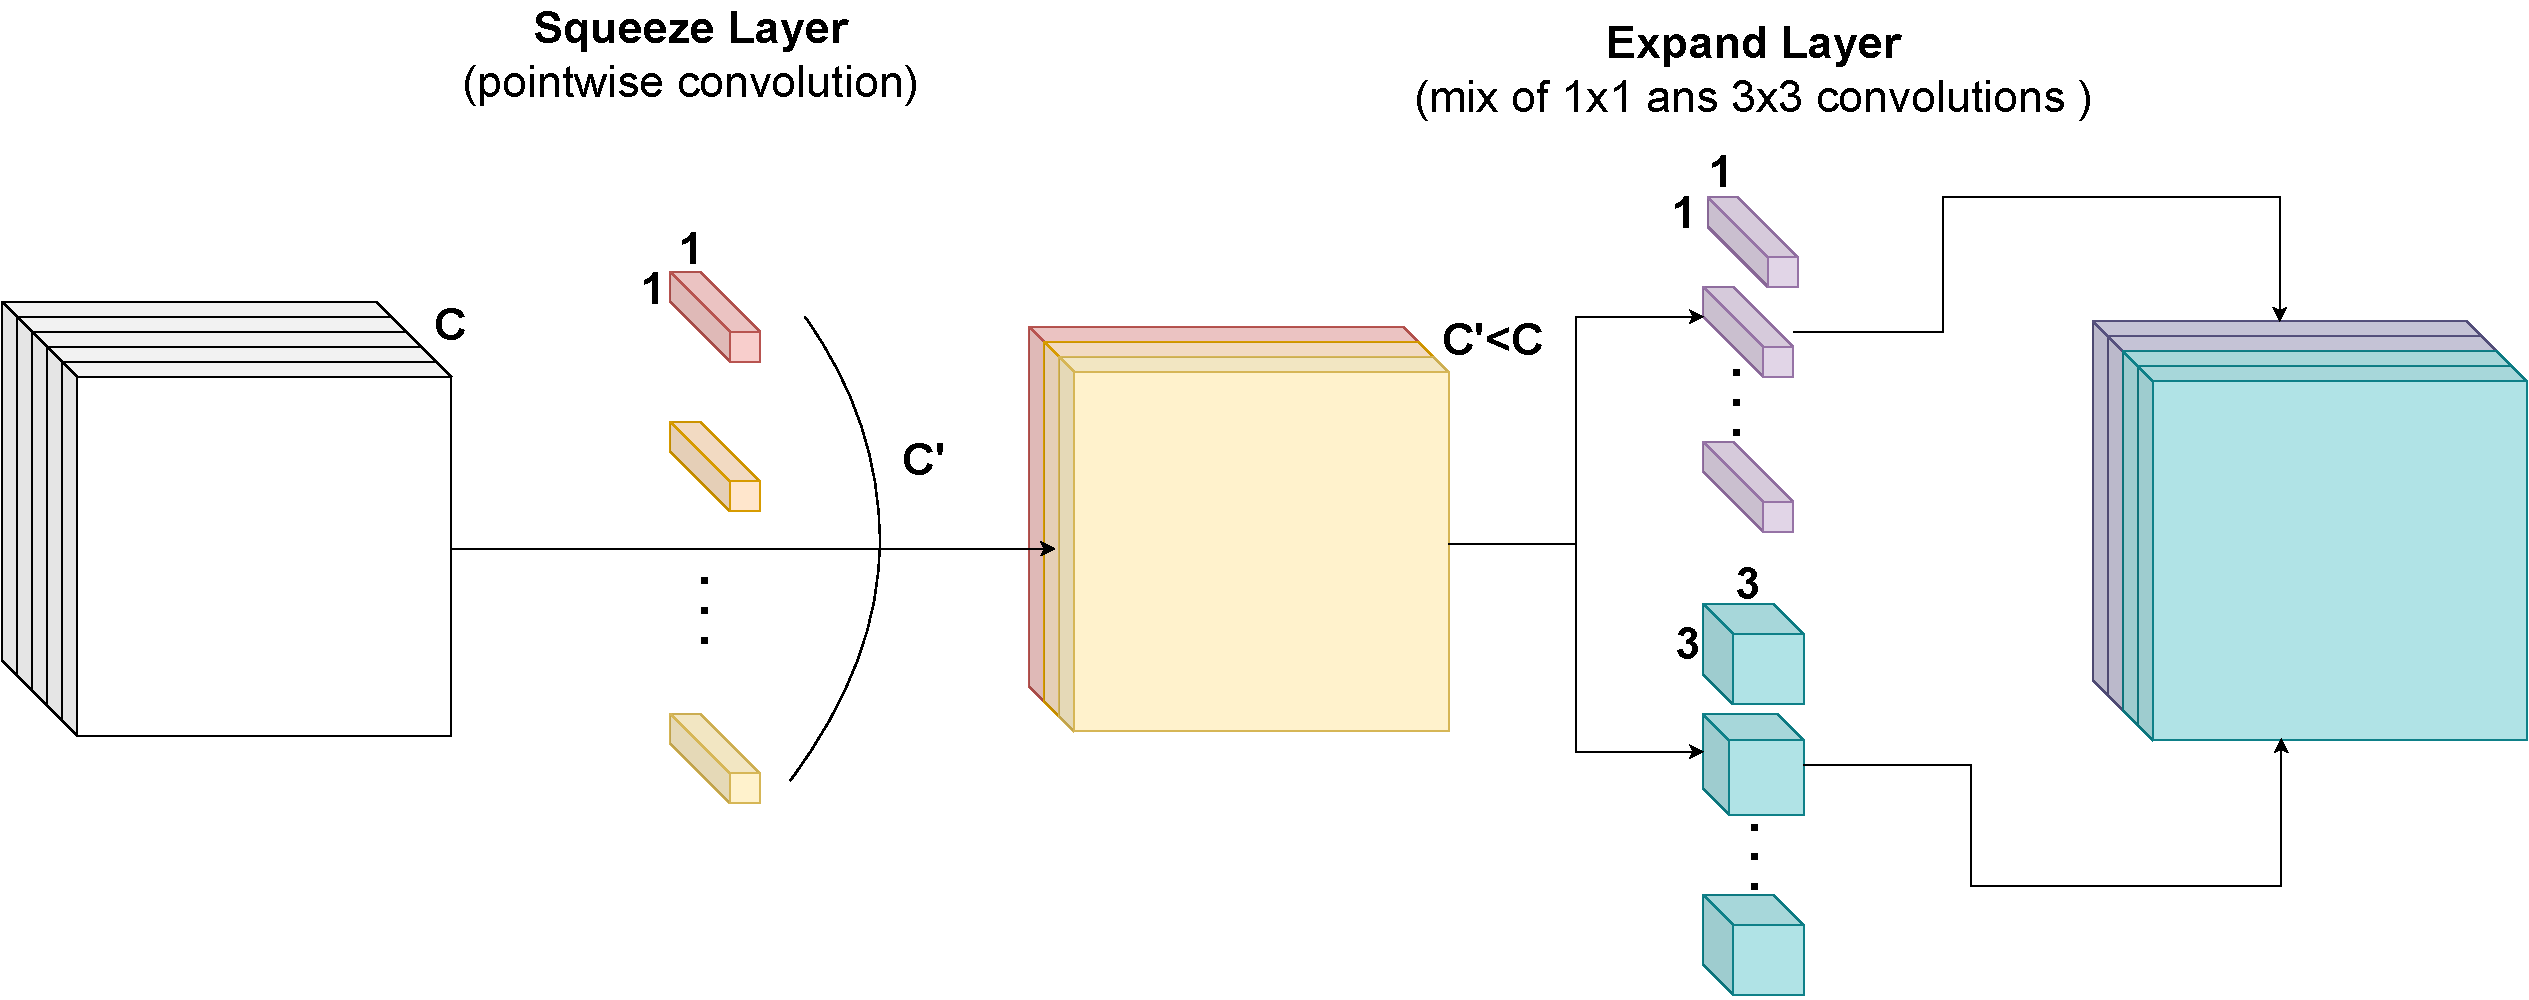
\includegraphics[width=0.70\textwidth]{chapter_sota/assets/fire_module.pdf}
    \caption{Illustration scheme of the fire module. The fire module is composed
    is composed of a \emph{squeeze layer} (pointwise convolution designed to
    reduce the number of channels fed to the following layer) and an
    \emph{expand layer} (convolution with mixed $1\times1$ and $3\times3$
    kernels. The $1\times1$ kernels replace some of the $3\times3$ kernels,
    being less computationally intensive.). Best viewed in colours.}
    \label{fig:sota:fire_module}
\end{figure}

% endregion: fire module

% region: shufflenet

Pushing the concept of depthwise separable convolutions further,
\cite{ZhangShuffleNet} introduces pointwise group convolutions and channel
shuffle operations to enhance efficiency while maintaining accuracy. Pointwise
group convolutions were initially introduced in
\cite{DBLP:conf/nips/KrizhevskySH12}, though their original purpose was not for
compression. Instead, group convolutions in \cite{DBLP:conf/nips/KrizhevskySH12}
were used to enable distributed training across multiple \acp{GPU} with limited
memory. However, ShuffleNet \cite{ZhangShuffleNet} leverages this concept for
network efficiency by dividing the input channels into groups and performing
convolutions on each group independently. This approach reduces the number of
operations and computational cost compared to traditional convolutions. To
counteract the potential loss of expressive power caused by the separation of
channels into groups, ShuffleNet incorporates \emph{channel shuffle operations}
as shown in \cref{fig:sota:shuffle_net}. This technique allows for information
exchange between groups, effectively maintaining accuracy by ensuring that
different groups can capture diverse features in the input.\\

\begin{figure}[htbp]
    \centering
    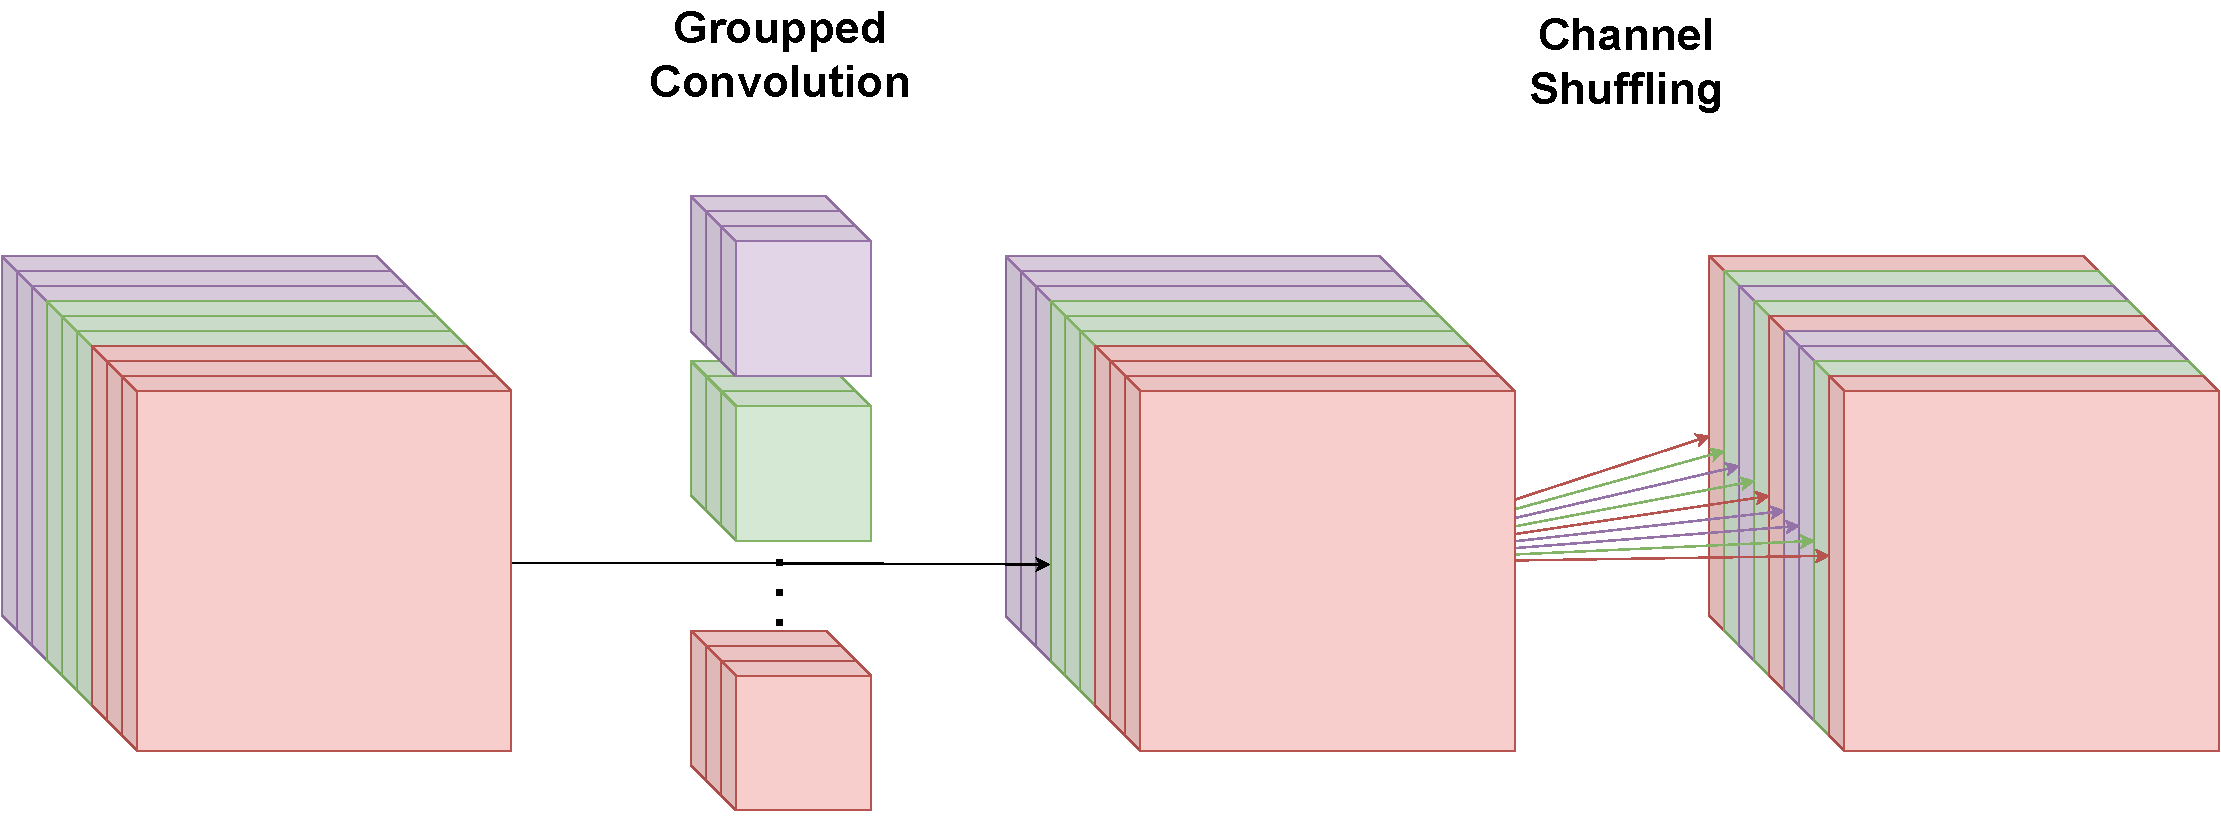
\includegraphics[width=0.70\textwidth]{chapter_sota/assets/group_conv_and_channel_shuffling.pdf}
    \caption{Illustration scheme of grouped convolution with channel shuffling.
    Each filter only acts on a subset of the input tensor (here represented by a
    matching colour). The channels of the yielded tensor are shuffled to ensure
    the subsequent groups can access information from all the previous groups. Best
    viewed in colours.}
    \label{fig:sota:shuffle_net}
\end{figure}

Following ShuffleNet, CondenseNet was introduced in \cite{huang2018condensenet},
incorporating learned group convolutions to further enhance efficiency. Unlike
the predefined group convolutions in ShuffleNet, CondenseNet learns which
channels should be grouped together, enabling the network to adapt its structure
for a specific task. This results in better utilisation of network capacity and
reduces redundancy. CondenseNet leverages the DenseNet architecture
\cite{huang2017densely} to further improve performance. Thanks to the densely
connected architecture, features discarded in any layer can still be recovered
in subsequent ones.\\

\begin{figure}[!h]
    \centering
    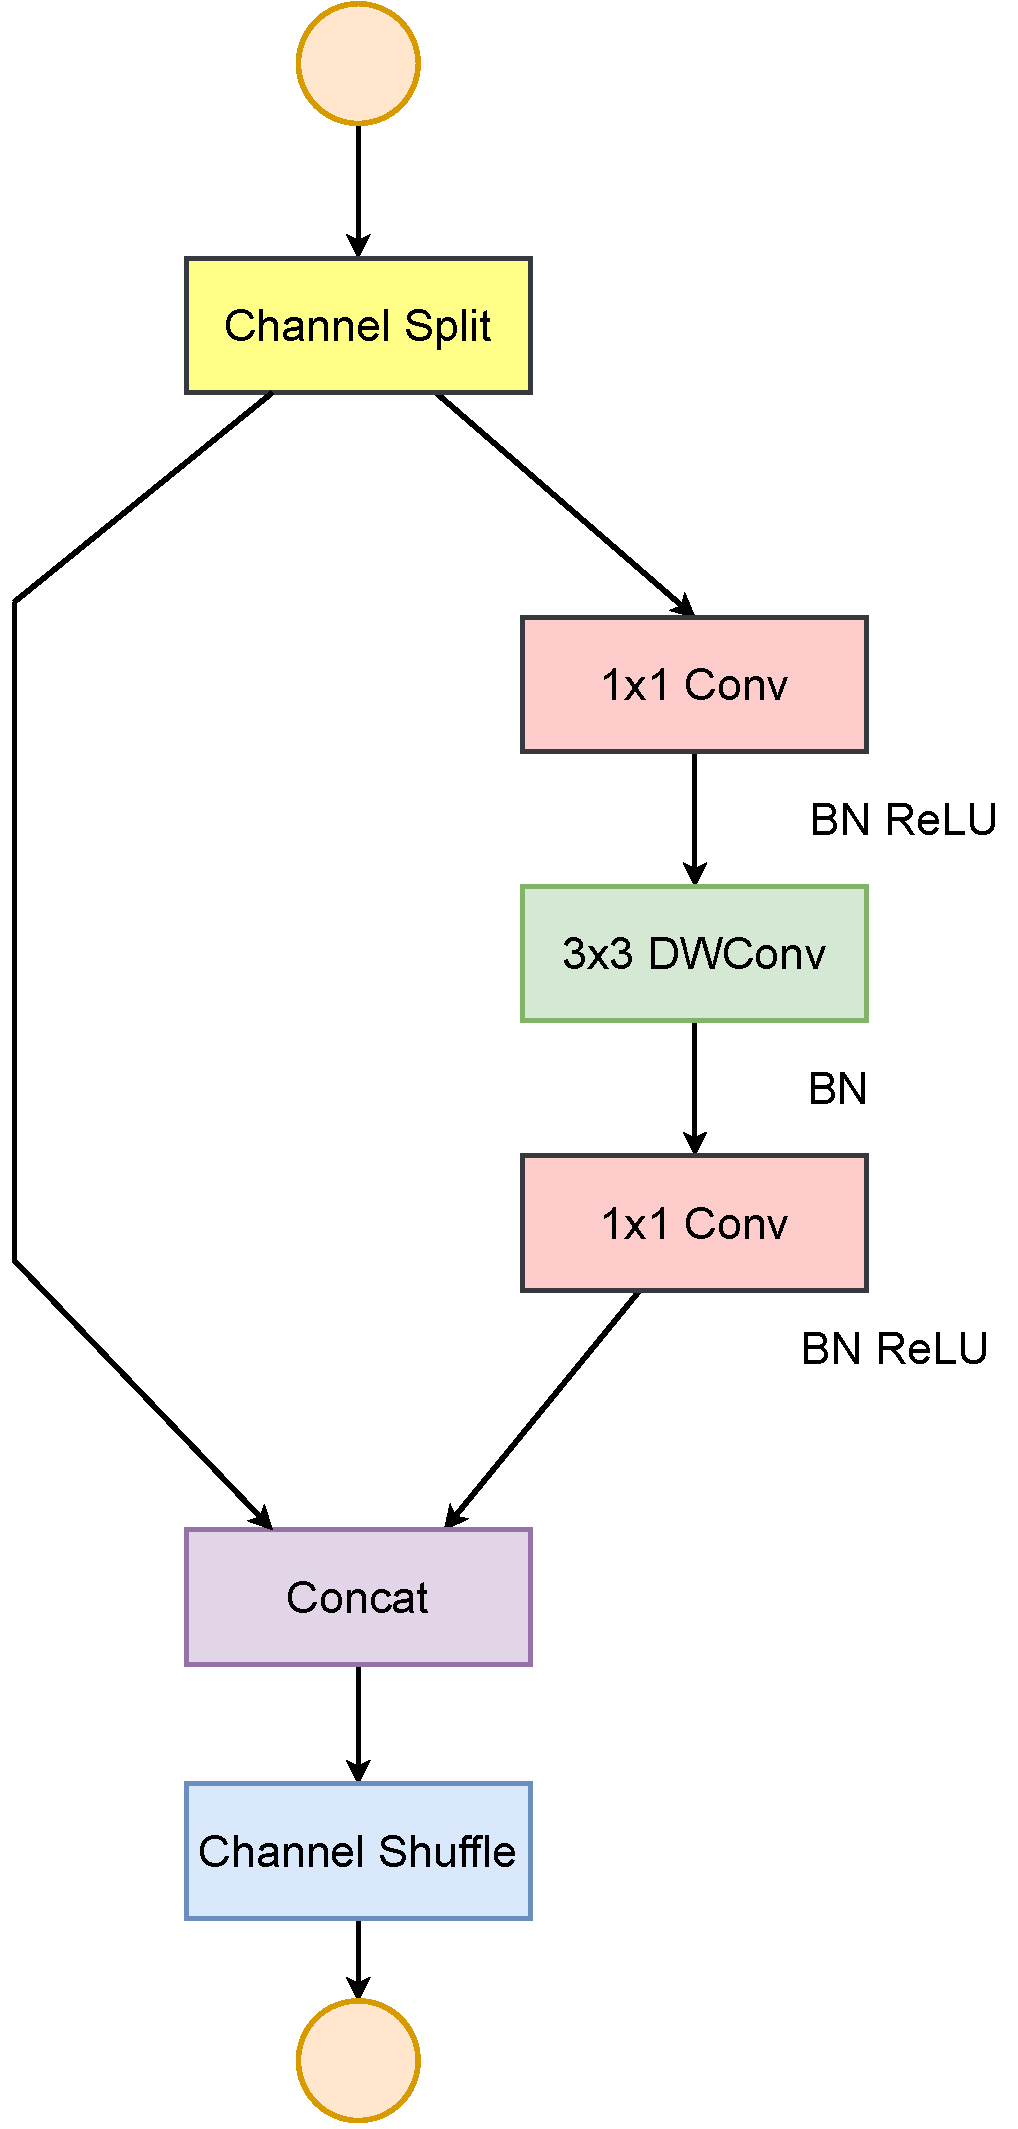
\includegraphics[width=0.3\textwidth]{chapter_sota/assets/channel_split.pdf}
    \caption{Illustration scheme of the path taken by the feature maps after the
    channel split block. Adapted from the original scheme found in \cite{MaShuffleNetV2}.}
    \label{fig:sota:channel_split}
\end{figure}

Building on the success of ShuffleNet, ShuffleNetV2 was introduced in
\cite{MaShuffleNetV2}, focusing on enhancing network efficiency through the
combination of strided convolution and channel split. Strided convolution helps
reduce the spatial dimensions of feature maps, thereby reducing the computation
cost. The Channel Split technique efficiently processes the input feature maps
while maintaining the expressive power of the architecture. Channel Split works
by dividing the input feature maps into two equal parts. One part is passed
through the main branch of the ShuffleNet unit, while the other part is sent
through the identity branch, which leaves its input unchanged. In the main
branch, a sequence of pointwise and $3\times 3$ convolutions are performed.
After both the main branch and the identity branch complete their respective
operations, the two parts are concatenated along the channel dimension and the
channels are shuffled. Finally, the output feature maps are passed to the next
ShuffleNet unit in the network. This process is represented in
\cref{fig:sota:channel_split}. This approach balances computational efficiency
with the expressive capacity of the model.\\
% endregion: shufflenet

% region: mobilenetv2
Depthwise Separable Convolutions were employed and improved in
\cite{howard2017mobilenets}. \citeauthor{DongMobileNetV2} introduced skip
connections and residual blocks into the MobileNet architecture, initially
proposed in \cite{DBLP:conf/cvpr/HeZRS16}. They also introduced the concept of
inverted residuals and linear bottlenecks. In conventional residual blocks, the
input is first compressed, then expanded, and finally compressed again after
being added to the original input. With inverted residual bottlenecks, on the
other hand, this process is reversed: the input is first expanded, then a
depthwise separable convolution is applied, and finally, it's compressed again.
In this architecture, the skip connections link the feature maps of smaller
size, instead of the larger ones. This allows for a more memory-efficient
architecture. The standard residual blocks and the inverted residual blocks are
shown in \cref{fig:sota:inverted_vs_residual_blocks}. The linear bottlenecks, on
the other hand, are convolutions without non-linear activation functions like
\ac{ReLU}. This takes advantage of the property that high-dimensional feature
maps can be embedded in a lower-dimensional manifold. To do this, it is
necessary to use linear transformations without an activation function, which
could potentially destroy information.\\

\begin{figure}
    \centering
    \subfloat[Standard Residual Block\label{fig:sota:residual_block}]{%
        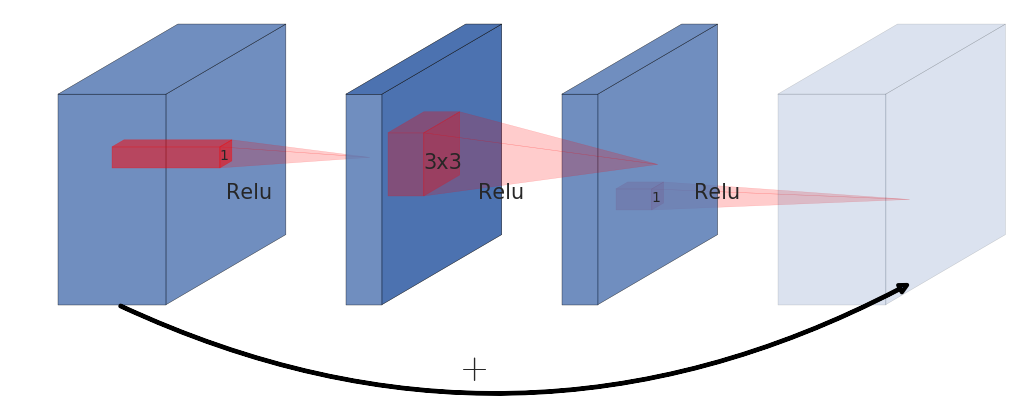
\includegraphics[width=0.49\textwidth]{chapter_sota/assets/mobilenet_v2_residual.png}}
    \subfloat[Inverted Residual Block\label{fig:sota:inverted_residual_block}]{%
        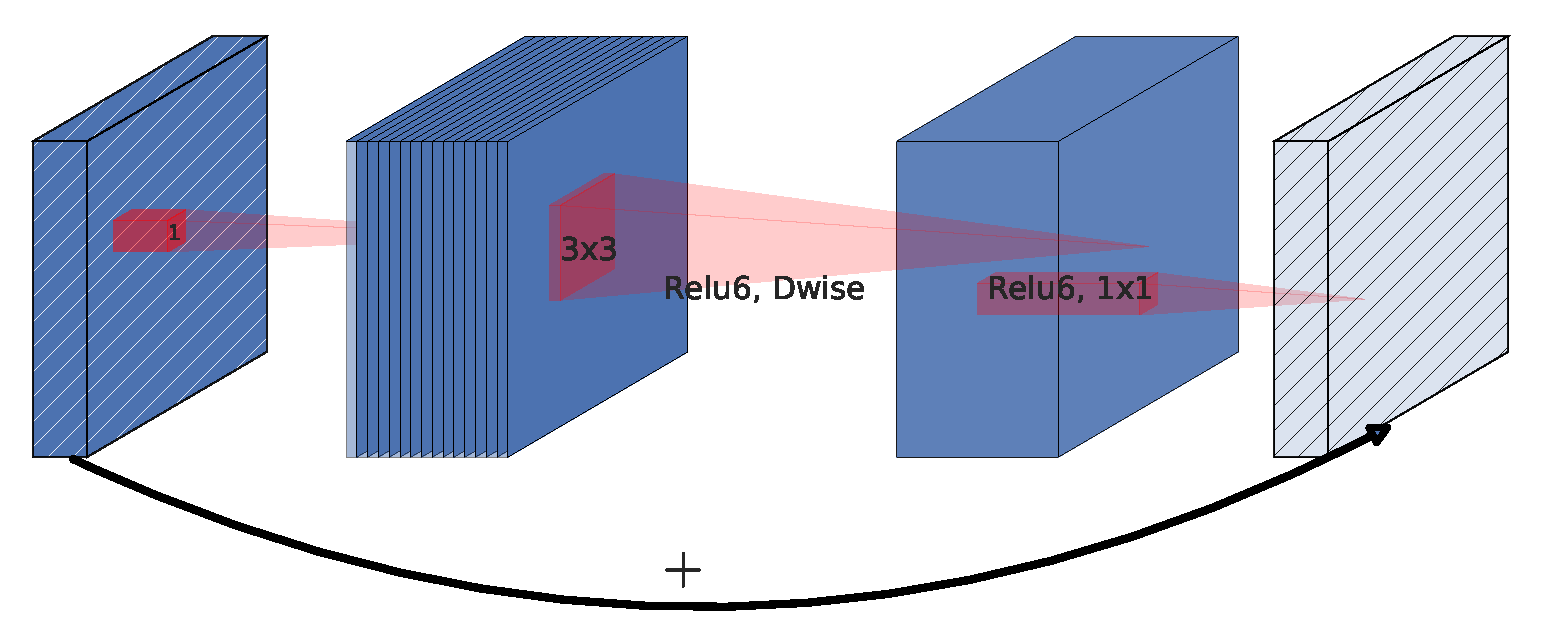
\includegraphics[width=0.49\textwidth]{chapter_sota/assets/mobilenet_v2_inverted_residual.pdf}}
    \caption{Illustration scheme of the residual block and the inverted residual
    block. Note that on the inverted residual block, the feature maps with the lower
    channel count are the ones connected via the skip connection, whereas it is the
    opposite on the standard residual block. Diagonally hatched layers do not use
    non-linearities. The grey colour indicates the beginning of the next block. Both
    illustrations are taken from \cite{DongMobileNetV2}. Best viewed in colours.}
    \label{fig:sota:inverted_vs_residual_blocks}
\end{figure}

% endregion: mobilenetv2

% region: mobilenetv3
Advancing from MobileNet and MobileNetV2, its third iteration
\cite{DBLP:conf/iccv/HowardPALSCWCTC19} incorporated \ac{SE} modules initially
introduced in \cite{DBLP:conf/cvpr/HuSS18}. These modules adaptively recalibrate
channel-wise feature responses, amplifying important features and suppressing
less relevant ones. The \ac{SE} module (represented in
\cref{fig:sota:se_module}) performs \emph{squeeze} and \emph{excitation}
operations. The squeeze operation uses global average pooling to create a
channel descriptor that summarises the spatial information for each channel. The
excitation operation uses this descriptor to learn non-linear interactions
between channels through two fully connected layers. The output of this
mini-network are per-channel modulation weights that recalibrate the original
feature maps, scaling or "exciting" them by these weights.\\

% endregion: mobilenetv3

\begin{figure}[htbp]
    \centering
    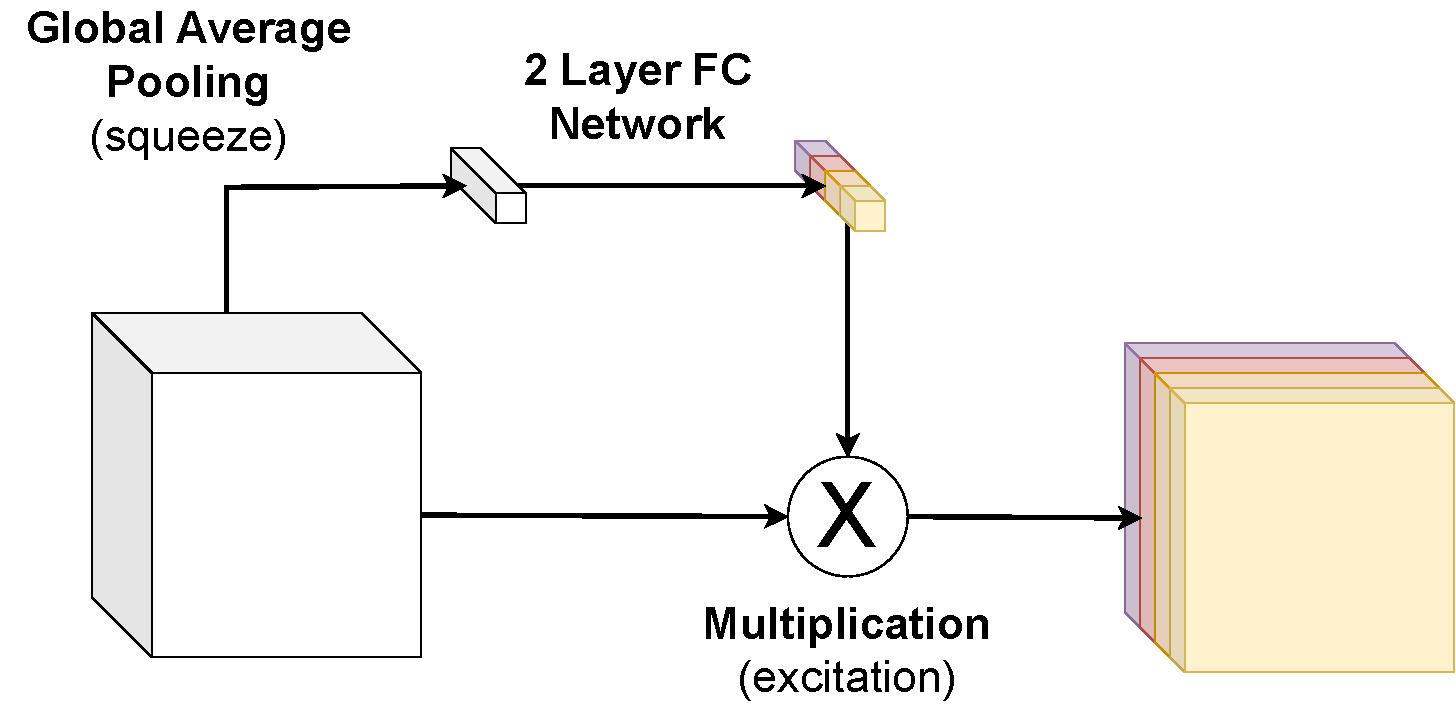
\includegraphics[width=0.70\textwidth]{chapter_sota/assets/SE_module.pdf}
    \caption{Illustration scheme of the \acf{SE} module. The original feature
    map is \emph{squeezed} into a channel descriptor through global average
    pooling. This descriptor is then used to learn the interdependencies between
    the channels through two fully connected layers. The output is then
    multiplied layerwise with the original feature map (\emph{excitation}). Best
    viewed in colours.}
    \label{fig:sota:se_module}
\end{figure}


% region: transition paragraph
The architectures we have just reviewed revolve around specific key techniques
such as depthwise separable convolutions, fire modules, channel shuffling, and
\ac{SE} modules, among others. These architectures, while highly efficient, are
manually crafted and require a significant degree of human expertise, intuition,
and time to develop, optimise, and fine-tune. The manual design of these
architectures often relies on a deep understanding of the tasks at hand, the
data they will process, and the constraints of the environment in which they
will operate. However, the process of designing these efficient architectures
can be automated, which is the subject of the next section. Sizes and
performance of networks architecture detailed in this section can be compared to
standard architecture sizes on \cref{fig:sota:net_sizes_std_eff}.\\

\begin{figure}[htbp]
    \centering
    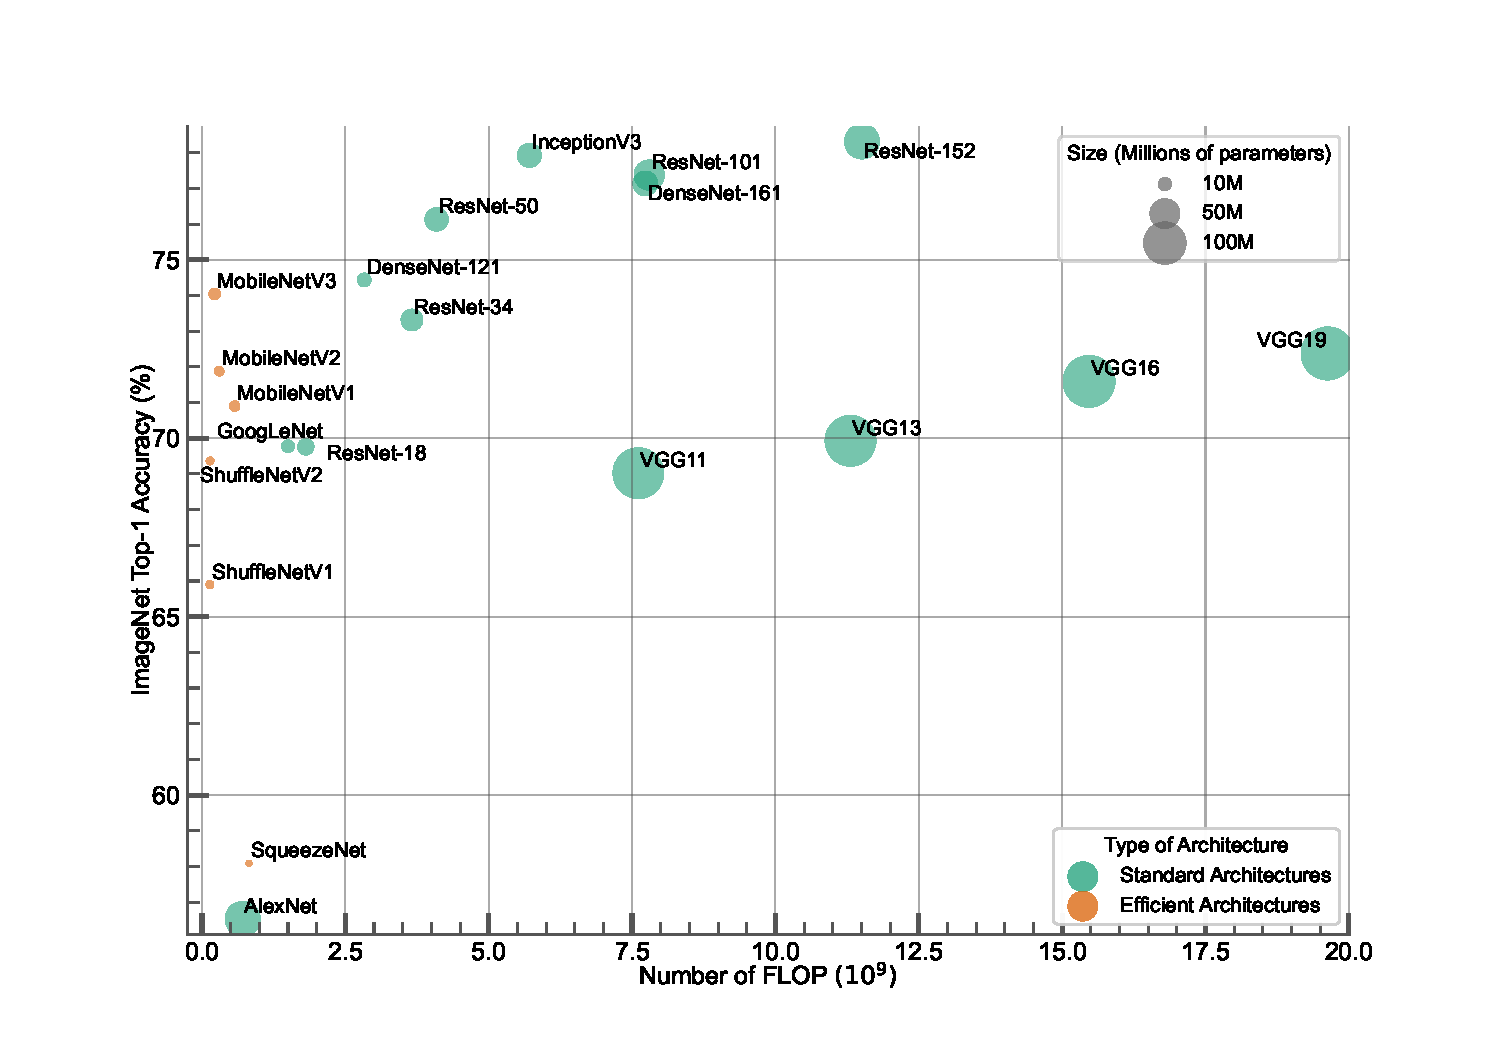
\includegraphics[width=0.70\textwidth]{chapter_sota/assets/network_sizes_normal_eff.pdf}
    \caption{\Cref{fig:sota:net_sizes} updated with the size and performance of the efficient
    architectures detailed in \cref{sec:sota:efficient_archi}}
    \label{fig:sota:net_sizes_std_eff}
\end{figure}




% endregion: transition paragraph

\subsection{Automatic Architecture Design Through Neural Architecture Search}
\label{sec:sota:nas} 

\acf{NAS} is a method that automates the discovery of neural network
architectures, potentially leading to more compact, efficient designs and
reducing the need for manual intervention. Although \ac{NAS} might not
explicitly aim at producing lightweight architectures, it can still yield
designs that strike a good balance between performance and computational cost
\cite{DBLP:conf/cvpr/TanCPVSHL19,DBLP:conf/icml/TanL19}. By using automated
methods to search for optimal architectures, it is possible to further enhance
the efficiency of neural networks, opening up new possibilities for their
deployment in resource-constrained environments. \ac{NAS} has emerged as an
essential paradigm, aiming to automate the traditionally manual and
labour-intensive process of designing efficient neural networks
\cite{DBLP:journals/corr/MiikkulainenLMR17}. Early network architectures were
indeed entirely handcrafted, requiring significant human effort and expertise.
However, these manual methods are being replaced by \ac{NAS} techniques, which
seek to automatically determine the optimal network structure given a training
set \cite{DBLP:journals/corr/abs-2301-08727,elsken2019neural}.\\

The performance and efficiency of \ac{NAS} are fundamentally determined by two
key aspects: the \emph{search space} and the \emph{search strategy}. The search
space, as the term suggests, defines the set of all possible architectures that
can be discovered by the \ac{NAS} algorithm. It could be as broad as all
possible configurations of a certain type of network, such as \acp{CNN}, or as
narrow as different arrangements of a specific set of layers
\cite{DBLP:conf/cvpr/LiuCSAHY019}. The search strategy, on the other hand,
determines how the \ac{NAS} algorithm navigates through this search space in
order to optimise its given objective. This could involve gradient-based
strategies \cite{DBLP:conf/iclr/LiuSY19,DBLP:conf/iclr/XuX0CQ0X20}, or
stochastic methods, such as evolutionary algorithms and reinforcement learning
strategies \cite{DBLP:conf/iclr/ZophL17,DBLP:conf/icml/RealMSSSTLK17}. The
choice of search space and search strategy significantly influences the ability
of \ac{NAS} to discover effective and efficient architectures, and is thus a
critical aspect of NAS research. In the following paragraphs, we will delve
deeper into some of these strategies and their impact on the field of
\ac{NAS}.\\



The search space is a critical aspect of \ac{NAS} as it bounds the possibilities
of architectures and significantly influences the outcome of the search. The
search space could be as broad as all possible configurations of a certain
network type or as specific as various arrangements of a predefined set of
layers or blocks. For instance, \cite{DBLP:conf/iclr/ZophL17} define their
search space as a set of repeatable sub-structures composed of basic layers
(convolution layers, fully connected layers, \ac{batch norm} layers, etc...)
often called \emph{cells} that are stacked to form the final architecture, while
\cite{DBLP:conf/iclr/XieZLL19} design their search space based on the
connectivity patterns between network blocks. \cite{DBLP:conf/iclr/LiuSY19}
propose a continuous search space where the architecture is parameterized as a
differentiable function, allowing for efficient search using gradient-based
methods. Hierarchical search spaces, on the other hand, offer a strategic
approach to navigate the complexity of the architecture search in \ac{NAS}
\cite{DBLP:conf/cvpr/LiuCSAHY019,DBLP:conf/cvpr/TanCPVSHL19}. In such a setup,
the architecture is divided into several levels of hierarchy, with each level
searched independently. This structure enables a more systematic and organized
exploration of the search space, allowing the algorithm to uncover useful
patterns and configurations at different levels of the network. The EfficientNet
models are exemplary of innovative architecture search strategies
\cite{DBLP:conf/icml/TanL19}. This series utilizes both \ac{NAS} and
\emph{compound scaling}. A baseline, EfficientNet-B0, was developed through
multi-objective \ac{NAS}, optimizing both accuracy and \acp{FLOP}. Subsequently, a
compound scaling method was applied to this baseline, uniformly scaling depth,
width, and resolution via a \emph{compound coefficient} $\phi$. This approach
yielded a series of progressively larger EfficientNet models, whose performances
are shown in \ref{fig:sota:efficientnet_perfs}.\\\


\begin{figure}[htbp]
    \centering
    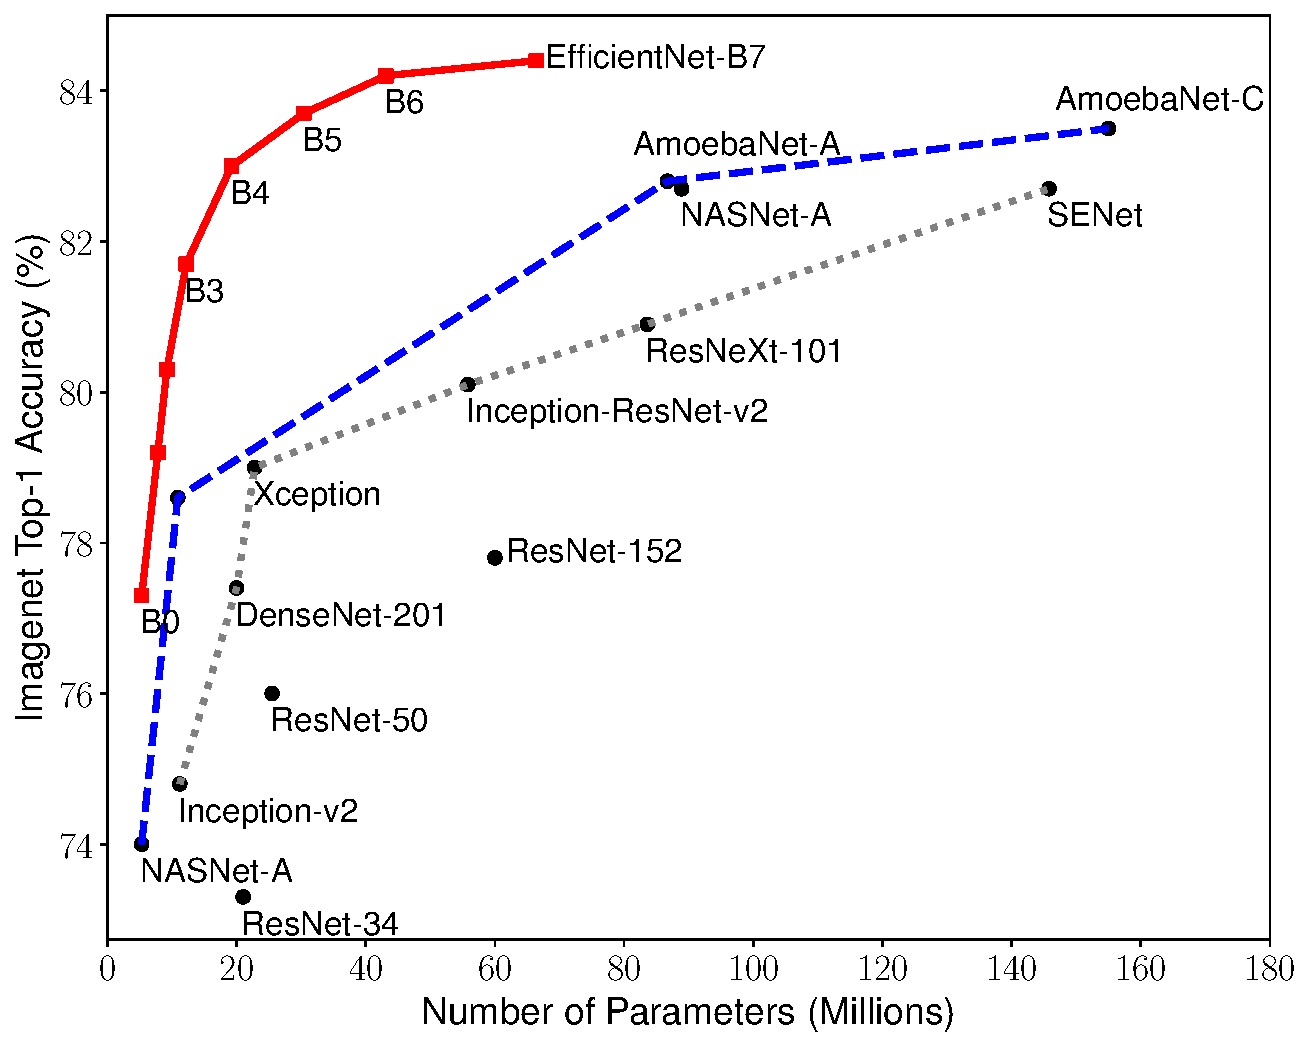
\includegraphics[width=0.70\textwidth]{chapter_sota/assets/efficientnet_perfs_overview.pdf}   
    \caption{ImageNet top-1 accuracy vs model size (in millions of parameters).
    The EfficientNet family of models significantly outperforms other models of
    similar size, obtained either by \ac{NAS} or manual design. This graph is
    taken from \cite{DBLP:conf/icml/TanL19}.
    }
    \label{fig:sota:efficientnet_perfs}
\end{figure}


The search strategy is another major component of \ac{NAS}, dictating how the
algorithm explores the search space to find the optimal architecture. A wide
range of search strategies have been proposed. Evolutionary algorithms
\cite{DBLP:conf/icml/RealMSSSTLK17} use principles of natural evolution such as
mutation, crossover, and selection to explore the search space. Despite their
potential to find high-quality solutions, these methods often require
substantial computational resources due to the large number of evaluations
needed. Reinforcement Learning-based methods \cite{DBLP:conf/iclr/ZophL17}
employ a policy network to generate architectures and a reward signal, typically
validation accuracy, to guide the search. While reinforcement learning methods
can effectively navigate large search spaces, their success heavily depends on
the quality of the reward signal. Gradient-based methods like
\cite{DBLP:conf/iclr/LiuSY19,DBLP:conf/iclr/XuX0CQ0X20} make the search space
continuous and use gradient descent for optimization, which enables efficient
exploration of the search space but requires careful regularization to prevent
overfitting. \cite{DBLP:conf/nips/BergstraBBK11} uses Bayesian optimization to
build a probabilistic model of the objective function and uses it to select
promising architectures, balancing exploitation and exploration. This method can
be sample-efficient but might struggle with high-dimensional spaces. These
diverse strategies offer multiple paths to navigate the complex landscape of
architecture search, each with its unique trade-offs between efficiency,
effectiveness, and computational demands.\\


\begin{figure}[htbp]
    \centering
    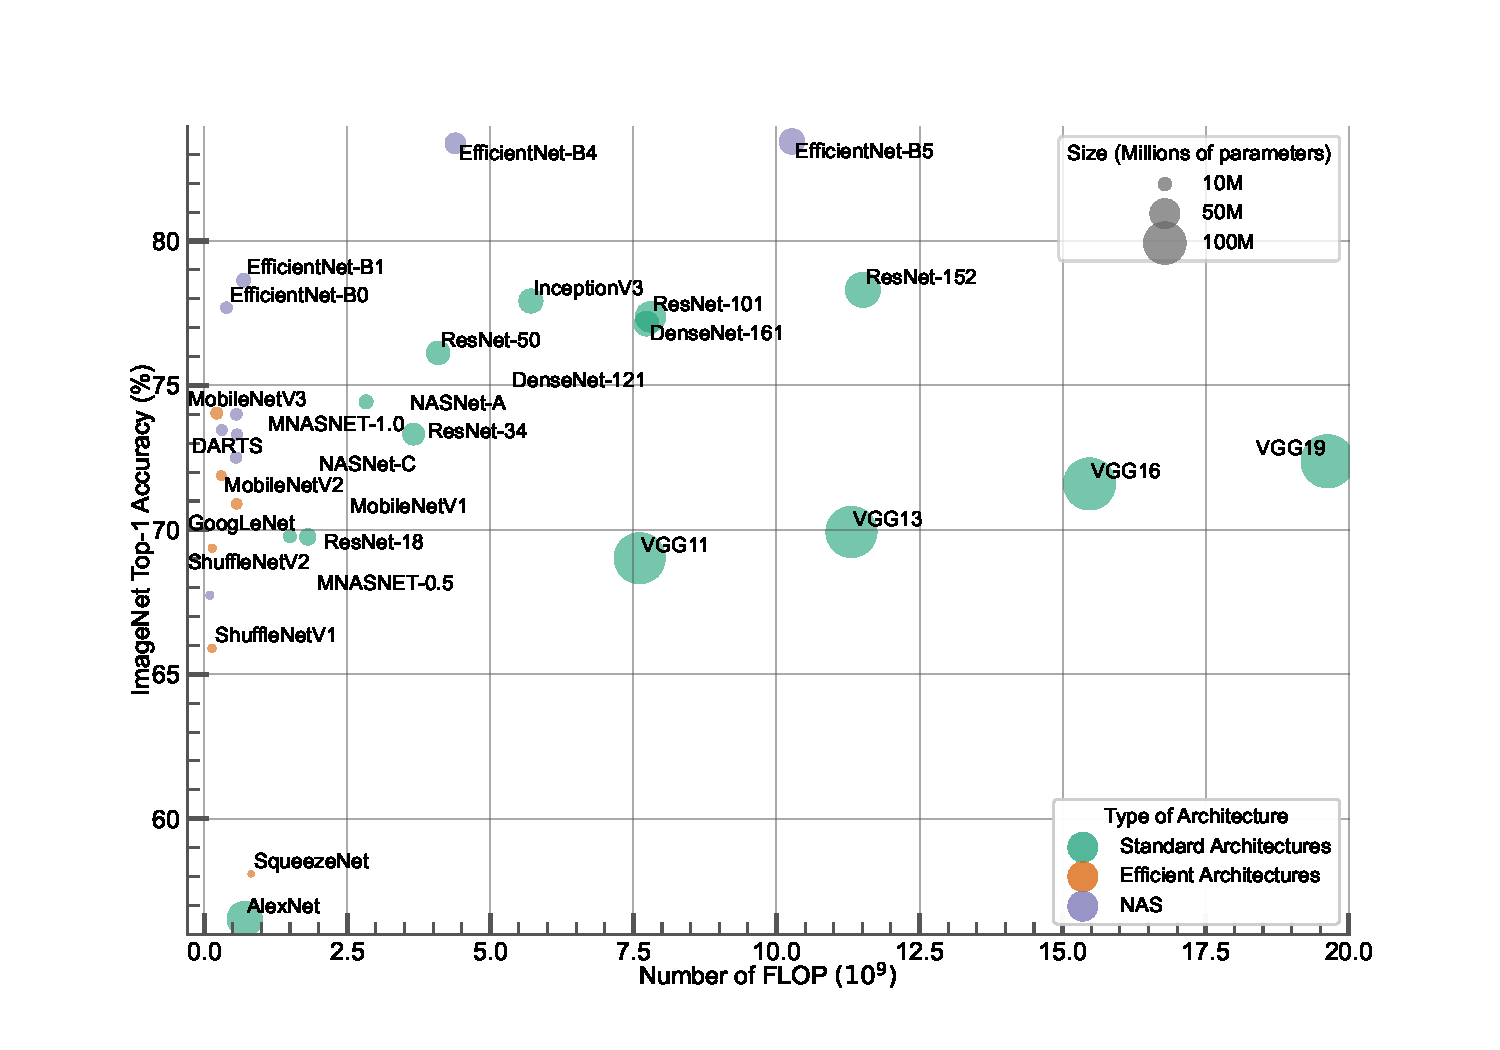
\includegraphics[width=0.70\textwidth]{chapter_sota/assets/network_sizes_normal_eff_nas.pdf}
    \caption{\Cref{fig:sota:net_sizes_std_eff} updated with the size and
    performance of architectures detailed in \cref{sec:sota:nas}}
    \label{fig:sota:net_sizes_std_eff_nas}
\end{figure}


\section{Architecture redfinement}

\subsection{Weight Operations}

\subsection{Pruning}



% ==============================================================================

\chapter{Weight Reparametrization}

\localtableofcontents

\begin{abstract}
    abstract of this part
\end{abstract}

\section{Introduction And Related Work}
% region
The introduction of neural networks has revolutionised the field of machine
learning, leading to breakthroughs in various areas such as image and speech
recognition, natural language processing, and game playing. However, the size of
neural networks has steadily increased in recent years, largely thanks to the
availability of powerful \ac{GPUs}. They have made it possible to train larger
and more complex models. However, as the size of neural networks has grown, so
have the computational and memory requirements to train and deploy them. The
evolution of neural network architectures can be traced back to the Rosenblatt
Perceptron \cite{rosenblatt1958perceptron}, a single-layer feedforward network
with only one neuron. Over time, neural network architectures became more
complex and included multiple layers, known as multi-layer perceptron or fully
connected networks. Then, with the introduction of \ac{CNNs}, neural network
architectures for image recognition have grown even larger. Convolutional neural
networks use convolutional layers to automatically and adaptively learn spatial
hierarchies of features from input images. This adaptivity allows \ac{CNNs} to
effectively learn and classify images with high accuracy. Some of the most
notable \ac{CNN} architectures include AlexNet
\cite{DBLP:conf/nips/KrizhevskySH12}, which was developed in 2012 and has 60
million parameters. The VGG networks \cite{DBLP:journals/corr/SimonyanZ14a},
developed in 2014, range from 132 to 143 million parameters. Inception
\cite{DBLP:conf/cvpr/SzegedyLJSRAEVR15}, developed in 2014, had 27 million
parameters in its third version. And the ResNet networks
\cite{DBLP:conf/cvpr/HeZRS16}, developed in 2015, are ranging from 11 to 60
million parameters. \\


The need for neural networks in embedded applications has grown in recent years.
Examples include object detection in self-driving cars, image and speech
recognition in mobile devices, and natural language processing in smart
speakers. These applications require real-time processing and low power
consumption, which are impossible with large neural networks. Pruning techniques
can reduce the size of neural networks, making them more suitable for deployment
on embedded devices while still maintaining or improving their performance.
Methods such as structured and unstructured weight pruning can reduce the number
of parameters and \ac{FLOPs}, consequently reducing the network's size, memory and
power consumption.\\


Pruning is an excellent way to obtain lightweight neural networks because it
reduces the number of parameters in a pre-trained network without the need to
design a new architecture from the ground up. Instead of starting from scratch,
pruning techniques can be applied to existing architectures, which have been
trained and tested on large-scale datasets. It aims to reduce the number of
network parameters by removing redundant or unnecessary weights. Pruning methods
can be split into two major categories: unstructured weight pruning, where
individual weights of the network are removed based on their importance. And
structured pruning, where entire columns, rows, channels, filters or even
subnetworks are removed. \\


The first methods to prune shallow networks were proposed in the late 1980s.
Techniques from that area include removing the smallest connection
\cite{janowsky1989pruning}, introducing a weight scaling factor and the study of
its impact on the loss function \cite{DBLP:conf/nips/MozerS88} or the study of
the sensitivity of the weights based on the gradients
\cite{DBLP:journals/tnn/Karnin90}. The most influential papers of the early
pruning days are Optimal Brain Damage \cite{DBLP:conf/nips/CunDS89} and Optimal
Brain Surgeon
\cite{DBLP:conf/nips/HassibiS92,DBLP:conf/nips/HassibiSW93,DBLP:conf/icnn/HassibiSW93}.
The former work focuses on pruning weights based on their impact on the loss,
approximated by its Taylor series, which requires the computation of the hessian
matrix of the loss. However, computing the hessian matrix is Intractable in
practice due to the large number of parameters in the neural networks.
Therefore, the authors introduced a few simplifying assumptions, most notably
the diagonal assumption for the hessian matrix: loss perturbations following
weight pruning are assumed to be weight independent. \\


More recently, pruning regained traction with the work of Han et al.
\cite{DBLP:conf/nips/HanPTD15}. The authors introduced a three-step pruning
method where first, the weights are tuned. Then all the weights whose absolute
value is below a certain threshold are removed. Finally, the remaining weights
are fine-tuned. \\


Following this work, research efforts stirred toward structured pruning.
Structured pruning removes groups of weights. The substructure of this group can
be a simple row or column in a filter, a channel of a filter, the filter itself
or even entire subnetworks. Structured pruning is not sparsifying weight tensors
but rather reshaping the network to remove unnecessary parts of it that are
costly to evaluate and do not bring much performance improvement regarding the
considered task. Since the remaining weight tensors are not sparse, speedups can
be achieved with conventional libraries and hardware. In this context, Anwar et
al. \cite{anwar2017structured} proposed a pruning technique on various levels
(channels, kernels and intra-kernel levels), while Li et al.
\cite{DBLP:conf/iclr/0022KDSG17} proposed a pruning method at a larger (filter)
level. Network slimming \cite{DBLP:conf/iccv/LiuLSHYZ17} is a streamlined
approach that aims at pruning the most useless channels in the layers preceding
\ac{batch norm} \cite{DBLP:conf/icml/IoffeS15}. It induces sparsity with
$\ell_1$ penalization of the \ac{batch norm} scaling factors, each one
associated with a channel. Then channels are removed based on the relative
importance of their associated scaling factor up to a predefined sparsity ratio.
More recent work proposed an automatic policy for pruning, such as \ac{amc}
\cite{DBLP:conf/eccv/HeLLWLH18}, which relies on reinforcement learning with two
interacting agents; the first one iterates over the layers of the architecture
and defines a targeted sparsity, and the second agent implements the targeted
sparsity using channel pruning. The \ac{amc} algorithm is either constrained by
accuracy or efficiency, depending on the reward assigned to the agents. Going
further with the concept of automatic pruning and architecture search,
Ramakrishnan et al. \cite{DBLP:conf/crv/RamakrishnanSN20} adapt $\ell_1$
penalisation from \cite{DBLP:conf/iccv/LiuLSHYZ17} to model the relative
importance of layers, groups of layers or network parts that can be removed.
Following the same line, \cite{DBLP:conf/icml/KangH20} proposed a channel
pruning method based on batch normalisation parameters. The authors introduce
masks that model the likelihood of feature maps being inhibited by the ReLU
activation function, thereby not contributing to the evaluation of the
underlying network. These masks are obtained by binarising the cumulative
density function of the gaussian distribution parameterised by the scaling and
the shift of the BN layer. Masks and BN parameters are updated "end-to-end" with
a gradient estimated using the Gumble Softmax trick
\cite{DBLP:conf/iclr/JangGP17}. Authors claim that a high accuracy is maintained
after pruning and without fine-tuning. \\



Although convenient to implement in practice, structured pruning imposes a
strong topological prior by removing whole chunks in the primary network and
achieves a lower sparsity rate compared to unstructured pruning. On the other
hand, unstructured weight pruning focuses on removing independent weights from
the global structure. As a result, this method is much more flexible and leads
to high sparsity rates and compression ratios. Han et al.
\cite{DBLP:conf/nips/HanPTD15} introduced a simple yet effective three-step
algorithm for unstructured weight pruning: a first standard training step to
identify the most important connections, a magnitude pruning step to remove the
smallest weight and a final fine-tuning step to compensate for the loss of
accuracy. \cite{DBLP:journals/corr/HanMD15} used the same technique in
combination with quantisation and Huffman coding, achieving a compression ratio
of up to 49x for a VGG16 network. Other methods do not rely on weight magnitude,
such as \cite{DBLP:conf/iclr/LouizosWK18}, which uses non-negative stochastic
gates as a surrogate L0 norm and penalises non-zero weights during training.
Variational Dropout \cite{DBLP:conf/icml/MolchanovAV17} introduces a
multiplicative gaussian noise as an alternative to binary dropout
\cite{DBLP:journals/corr/abs-1207-0580,DBLP:journals/jmlr/SrivastavaHKSS14} with
an unbound dropout rate. Magnitude pruning regains significant attention after
the publication of the Lottery Ticket Hypothesis
\cite{DBLP:conf/iclr/FrankleC19}ttery Tickets, whose training with initial
weights taken from the large networks yields comparably accurate classifiers. To
extract the lottery ticket, it is necessary to train the large network up to
convergence, apply magnitude pruning and restore the original values of the
unpruned weights. This Lottery Ticket can then be trained to match the level of
performances of the large network, with at most the same number of epochs
needed. Although remarkable, this result is hardly applicable in practice since
it requires multiple computationally intensive training steps.\\


These structured or unstructured methods propose different saliency indicators
and pruning criteria that aim at identifying and removing redundant or
unnecessary weights or groups of weights in order to remove them. Removing
weights introduces a loss of functional performance - depending on the task
considered - that needs to be compensated for (with the exception of
\cite{DBLP:conf/icml/KangH20}). This is achieved through fine-tuning the sparse
or lightened networks obtained after applying the pruning criterion. Fine-tuning
is a computationally intensive task and requires additional training time.
Moreover, the amount of weights pruned is enforced after the initial training,
meaning that the final target size or weight budget is never considered in the
optimisation procedure. Hence the need for a fine-tuning step. \\


In order to address the aforementioned issues, we introduce a novel
reparametrisation that learns not only the weights of a surrogate lightweight
network but also its topology. This reparametrisation acts as a regulariser that
models the tensor of the parameters of the surrogate network as the Hadamard
product of a weight tensor and an implicit mask. The latter makes it possible to
implement unstructured pruning constrained with a budget loss that precisely
controls the number of non-zero connections in the resulting network.
Experiments conducted on the CIFAR10 and the TinyImageNet classification tasks,
using standard primary architectures (namely Conv4, VGG19 and ResNet18), show
the the ability of our method to train effective surrogate pruned networks
without any fine-tuning.

% endregion

\section{Pruning With Weight Reparametrisation And Budget Loss}
% region
Consider the general case of a multi-layer neural network, denoted as a function
$f$ of two variables: $\theta$ and $X$. $f$ can be seen as the topology of the
network: a computation graph whose edge values are given by $\theta$. Indeed,
$\theta$ is the set of weights of the network: $\theta = \{\mathbf{w}_1,
\mathbf{w}_2, \ldots, \mathbf{w}_L\}$, where $L$ is the number of layer of the
network. $X$ is the input taken by the network. The input $X$ is an element of a
dataset $\mathcal{D}=\{ \mathcal{X}, \mathcal{Y} \}$, where $\mathcal{X}$ is the
set of the input data, and $\mathcal{Y}$ is the set of the corresponding labels.
The elements of $\mathcal{X}$ and $\mathcal{Y}$ are real-valued tensors.

\begin{equation}
    % \centering
    \begingroup
  \setlength\arraycolsep{0pt}
  f \colon\begin{array}[t]{c >{{}}c<{{}} c}
             \mathbb{R}^{\dim (X)} & \to & \mathbb{R}^{\dim (y)} \\ 
             X & \mapsto & f(X, \theta) = \hat{y} 
          \end{array}
  \endgroup
\end{equation}

Evaluating the neural network $f(X_i, \theta)$ yields the output $\hat{y_i}$
which is the prediction of the network for the input $X_i$. The discrepancy
between the output of the neural network $\hat{y_i}$ and the ground truth $y_i
\in \mathcal{Y}$ is computed with a loss function $\mathcal{L}$. This loss is
then minimised by updating the parameters $\theta$ of the network, thanks to the
backpropagation \cite{rumelhart1985learning,rumelhart1986learning} and gradient
descent methods.\\

The $L_0$ norm is perfectly suited for introducing sparsity in a network by, on
the one hand, acting as a sparsity-inducing regulariser for the weights, and on
the other hand, by indicating the number of non-zero weights in the network,
which is useful for computing the weight budget. \\

We aim to propose an end-to-end method that fits into the backpropagation
framework. Therefore, adding a $L_0$ regulariser and a $L_0$ based weight budget
is not possible since $L_0$ norm is not differentiable. Thus we propose our
differentiable reparametrisation, which seeks to define a novel weight
expression related to magnitude pruning
\cite{DBLP:conf/nips/CunDS89,DBLP:conf/nips/HanPTD15}. This expression
corresponds to the Hadamard product involving a weight tensor and a function
applied entry-wise to the same tensor (as shown in
\cref{fig:chap1:comparison_reparam_vs_mag_pruning}). This function acts as a
mask that \emph{(i)} multiplies weights by soft-pruning factors which capture their
importance and \emph{(ii)} pushes less important weights to zero through a particular
budget added to the loss function $\mathcal{L}$. \\

\begin{figure}[h]
    \centerline{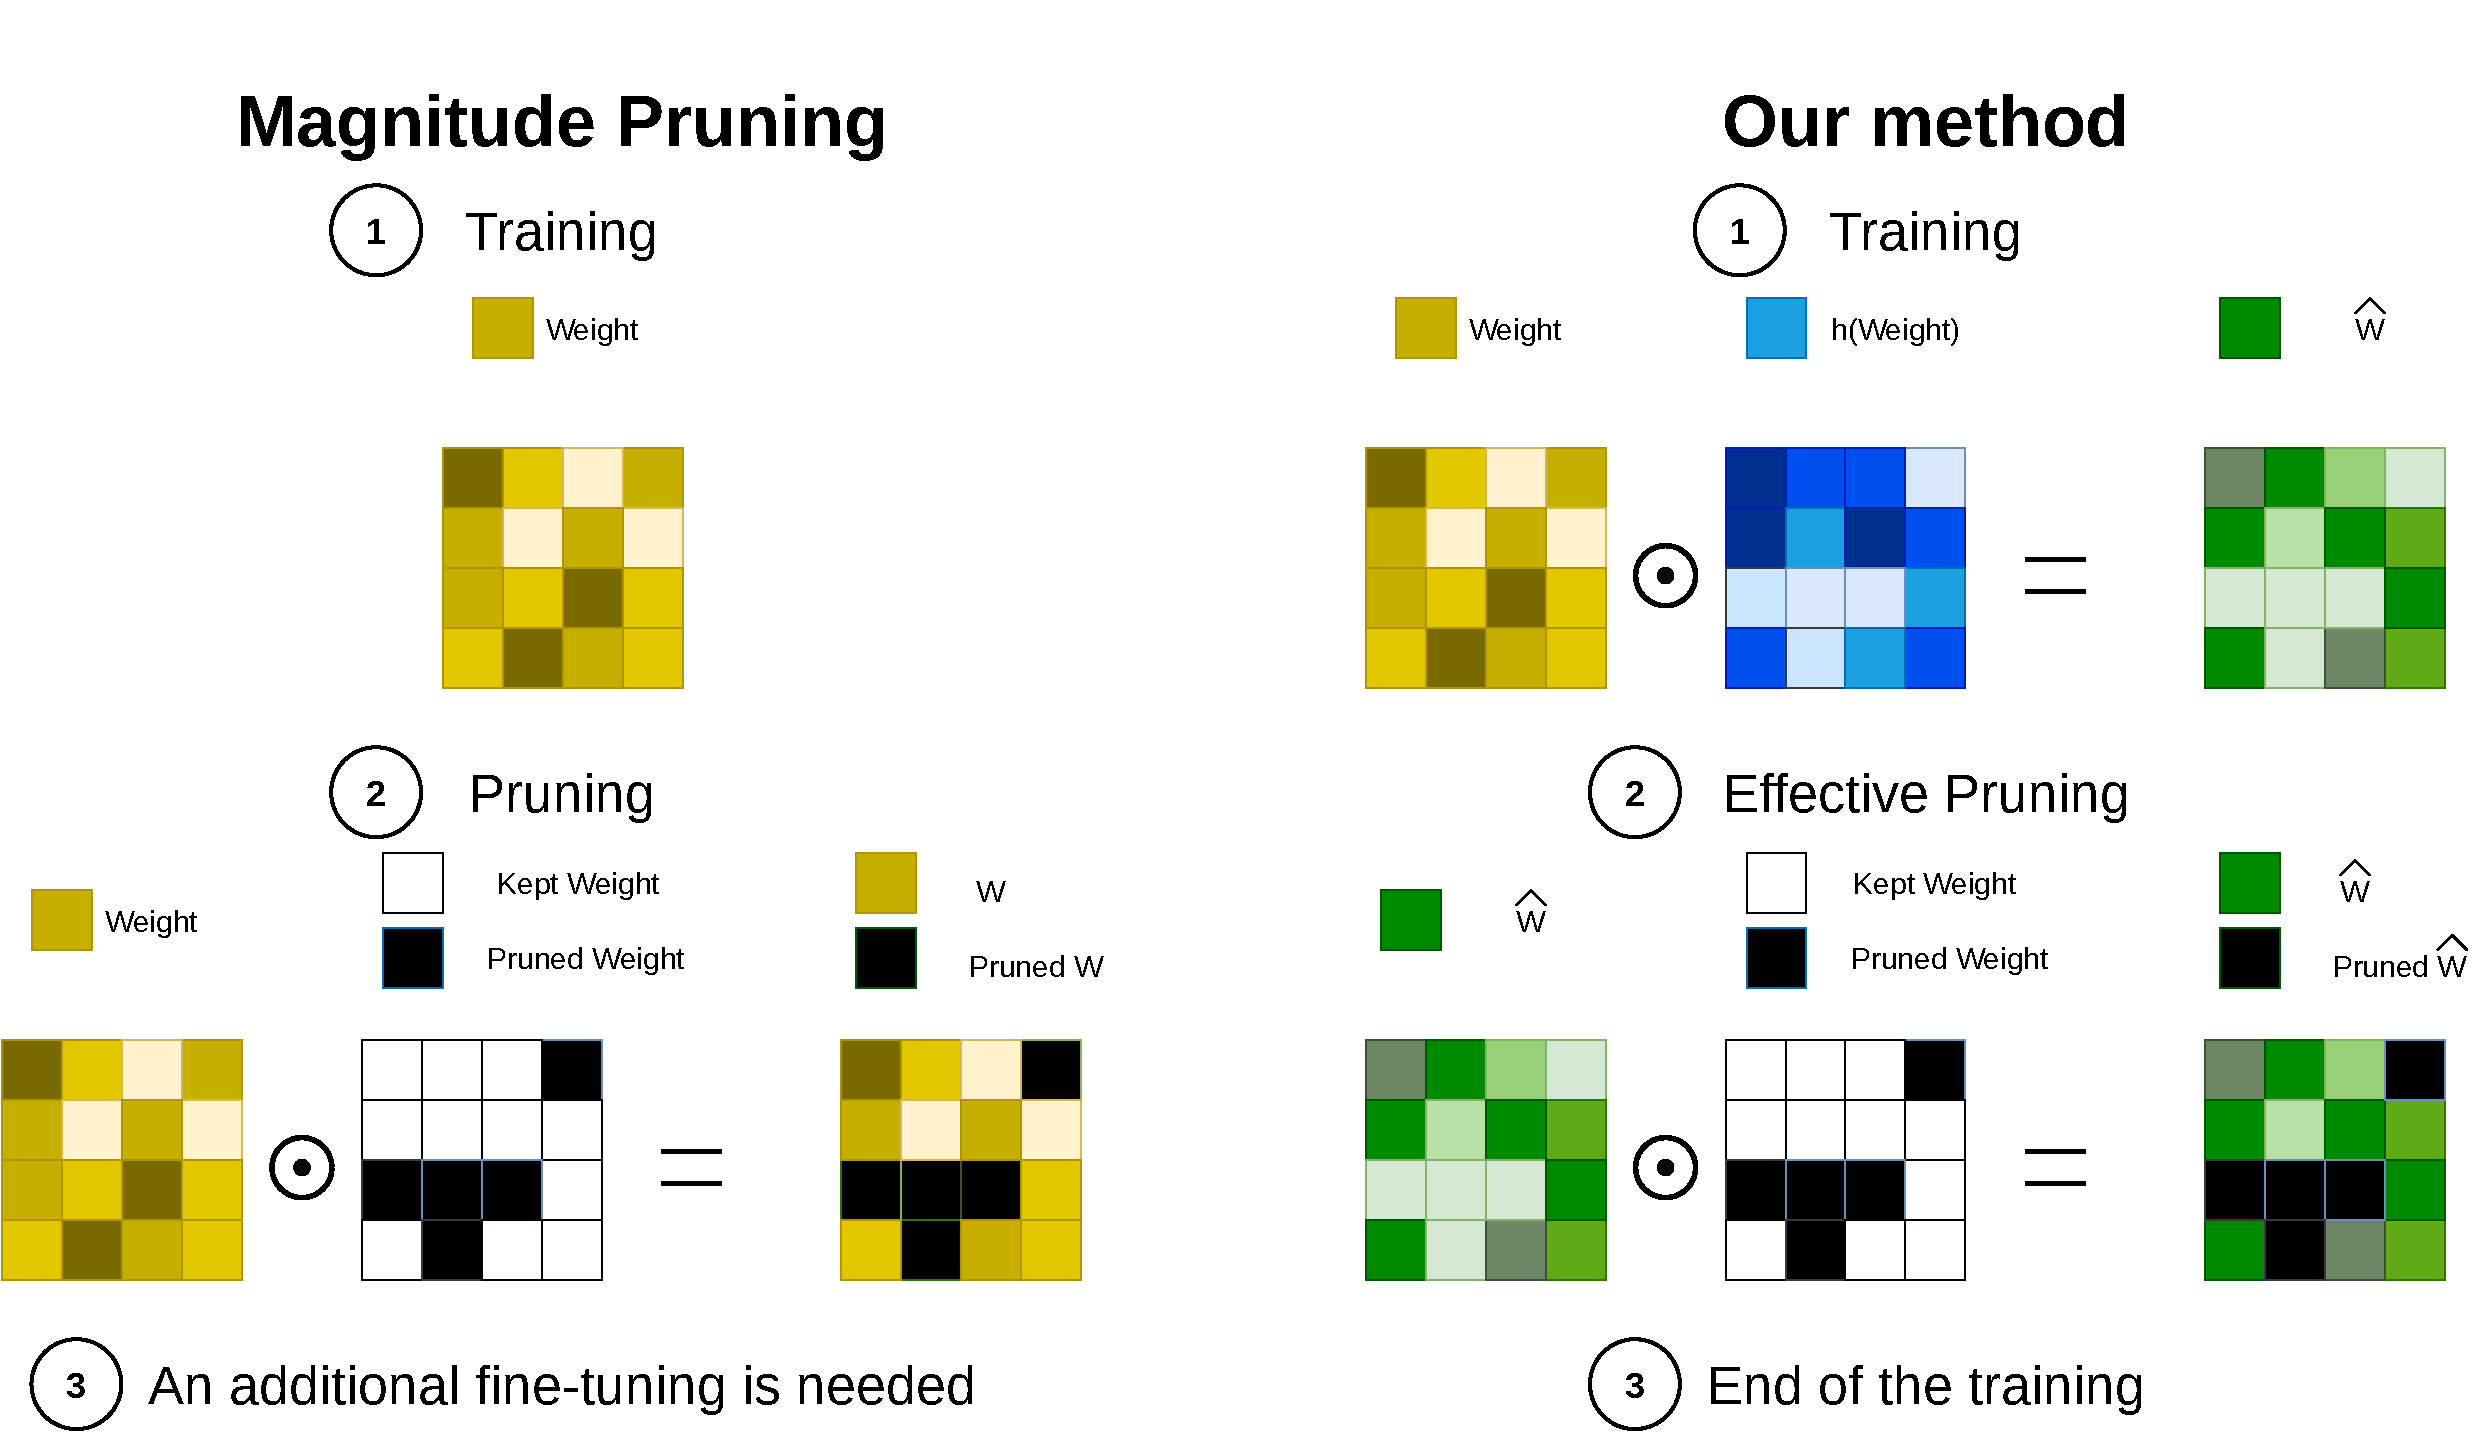
\includegraphics[width=12.5cm]{chapter_1/assets/comparison_reparam_vs_mag_pruning.pdf}}
  \caption{Comparison of our method and magnitude pruning. Magnitude pruning
  does not include any prior on weights during the initial training phase
  and needs an additional fine-tuning procedure. Our method embeds a saliency
  heuristic based on the weight magnitude in the weight reparametrisation and
  does not require fine-tuning.}
  \label{fig:chap1:comparison_reparam_vs_mag_pruning}
\end{figure}


Our proposed framework allows for a joint optimisation of the network weights
and topology. On the one hand, it prevents disconnections which may lead to
degenerate networks with an irrecoverable performance drop. On the other hand,
it allows reaching a targeted pruning budget in a more convenient way than $L_1$
regularisation. Our reparametrisation also helps minimise the discrepancy
between the primary and the surrogate networks by maintaining competitive
performances without fine-tuning. Learning the surrogate network requires only
one step that achieves pruning as a part of network design. This step zeroes out
the targeted number of connections by constraining their reparametrised weights
to vanish.

\subsection{Weight Reparametrization}
\label{sec:chap1:weight_reparam}

We consider the primary network $f$ as a combination of $L$ layers. The global
expression of $f$ can be recursively defined by the application of the layer $\ell$
to the output of the layer $\ell-1$. Without a loss of generality, we omit the
bias for clarity. This expression is shown on
\cref{eqn:chap1:layer_eq_f}.
\begin{equation}
\label{eqn:chap1:layer_eq_f}
f(\mathbf{x}) = g_L \big(\mathbf{w}_L \cdot g_{L-1}(\mathbf{w}_{L-1} \cdot g_{L-2} \dots
\mathbf{w}_2 \cdot g_1(\mathbf{w}_1 \cdot \mathbf{x}))\big),
\end{equation}
\noindent with $g_\ell$ being a nonlinear activation associated to $\ell \in
\left\{ 1,\dots, L \right\}$ and $\left\{ \mathbf{w}_\ell \right\}_\ell$ a
weight tensor. Keeping the same topology but changing the values of the weight,
we now consider the surrogate network $\hat{f}$ with weights
$\{\hat{w}_\ell\}_\ell$. \Cref{eqn:chap1:layer_eq_f} now becomes
\cref{eqn:chap1:layer_eq_f_hat}. The activation function and the topology of $f$
and $\hat{f}$ are the same. Only the weights are changing.

\begin{equation}
\label{eqn:chap1:layer_eq_f_hat}
\hat{f}(\mathbf{x}) = g_L \big(\mathbf{\hat w}_L \cdot g_{L-1}(\mathbf{\hat w}_{L-1} \cdot g_{L-2}
\dots\mathbf{\hat w}_2 \cdot g_1(\mathbf{\hat w}_1 \cdot \mathbf{x}))\big).
\end{equation}

\noindent In the above \cref{eqn:chap1:layer_eq_f_hat}, $\mathbf{\hat w}_\ell$
is referred to as apparent weight. The apparent weight is a reparametrisation of
$\mathbf{w}_\ell$, that includes a prior on its saliency. An apparent weight
$\mathbf{\hat w}_\ell$ of $\hat{f}$ is derived from the standard weight
$\mathbf{w}_\ell$ of $f$ by applying the following reparametrization: 
\begin{equation}
  \label{eqn:reparam}
  \mathbf{\hat w}_\ell = \mathbf{w}_\ell  \odot h_t(\mathbf{w}_\ell),
\end{equation}
\noindent with $h_t$ being the reparametrization function and $t$ its
temperature parameter. Here, $\odot$ represents the Hadamar product. It means
that the reparametrisation is element-wise, and every single weight has its own
reparametrisation. This reparametrisation function enforces the prior that
smallest weights should be removed from the network and act as a surrogate $L_0$
norm for the budget loss (see \cref{sec:chap1:budget_loss}). In order to achieve
this objective, $h_t$ should exhibit four properties: \\

\begin{enumerate}
  \item $\forall x \in \mathds{R},~~ 0 \leq h_t(x) \leq 1 $
  \item $h_t(x) \in C^1 \text{ on } \mathds{R}$
  \item $h_t(x) = h_t(-x)$
  \item $\forall a,\varepsilon \in\mathds{R}^{+\ast},~ \exists ~t
  \in\mathds{R}^{+\ast} ~ | ~ h_t(x) \leq \varepsilon, x \in [-a,a]$
\end{enumerate}

\noindent\textbf{First Property - Constrained Image} \\
\begin{equation}
    \centering
    \forall x \in \mathds{R},~~ 0 \leq h_t(x) \leq 1
    \label{eqn:chap1:reparam_prop1}
\end{equation}
\\
There should not be any co-adaptation between the weights and their
reparametrisation. Indeed, the reparametrisation function should not act as a
scaling factor for the weight and scale it so that the apparent weight is larger
than the original weight. Finally, the apparent weight should have the same sign
as the original weight. That is why the image of $\mathbb{R}$ by $h_t$ should be
the segment $[0,1]$.\\

\noindent\textbf{Second Property - Differentiability} \\
\begin{equation}
    \centering
    h_t(x) \in C^1 \text{ on } \mathds{R}
    \label{eqn:chap1:reparam_prop2}
\end{equation}
\\
Our method should fit in the backpropagation method. Since the optimisation will
be achieved by gradient descent, the reparametrisation function should be
derivable to ensure a computable gradient.\\

\noindent\textbf{Third Property - Symmetry} \\

\begin{equation}
    \centering
    h_t(x) = h_t(-x)
    \label{eqn:chap1:reparam_prop3}
\end{equation}
\\
The reparametrisation function should not induce any bias toward the positive or
negative weights so that only their magnitudes matter. It implies that the
reparametrisation function should be symmetric with respect to the origin.\\


\noindent\textbf{Fourth Property - Upper Bounded Segment} \\

\begin{equation}
    \centering
    \forall a,\varepsilon \in\mathds{R}^{+\ast},~ \exists ~t
    \in\mathds{R}^{+\ast} ~ | ~ h_t(x) \leq \varepsilon, x \in [-a,a]
    \label{eqn:chap1:reparam_prop4}
\end{equation}
\\
The last property ensures the existence of a temperature parameter $t$, which
allows upper-bounding the response of $h_t$ on any interval for any arbitrary
$\varepsilon$. More formally, for any arbitrarily large $a$ and arbitrarily
small $\varepsilon$, it exists a temperature $t$ which guarantees that the
reparametrisation of any $x$ is smaller than $\varepsilon$, provided that $x$ is
in the segment $[-a, a]$. Hence, $h_t$ acts as a stopband filter, eliminating
the smallest weights where the parameter $t$ controls the width of that filter.
\\



\begin{figure}
    \centering
    \subfloat[$h_{t}$ with $t=1$ and varying $n$]{
        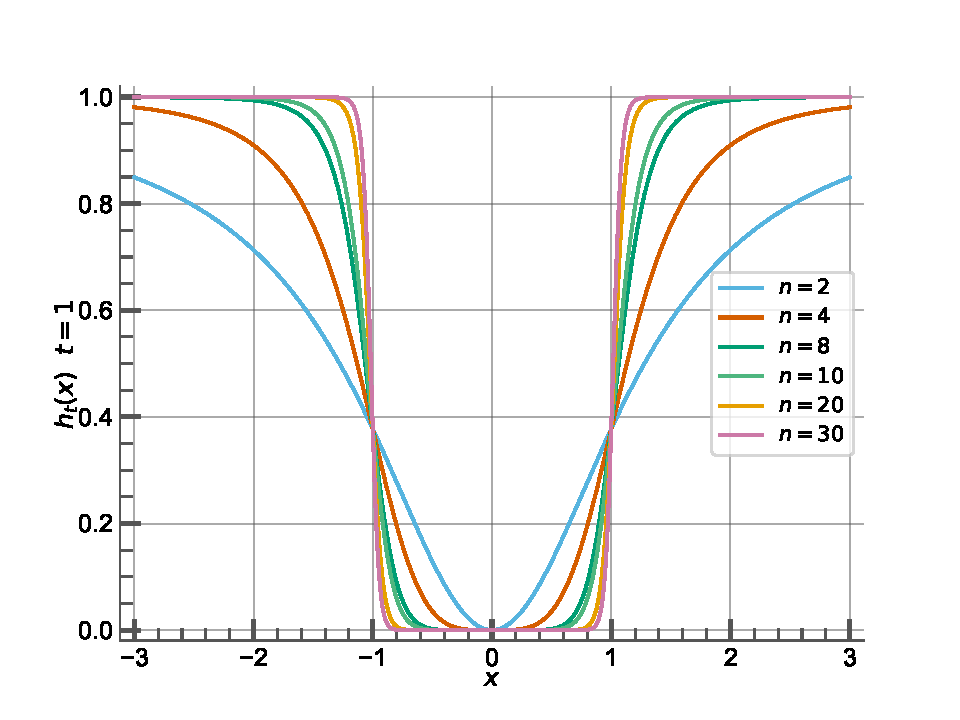
\includegraphics[width=0.49\linewidth]{chapter_1/assets/reparam_funct_varying_n.pdf}
        \label{fig:chap1:reparam_funct_varying_n}} \subfloat[$h_{t}$ with $n=2$
    and varying $t$]{
        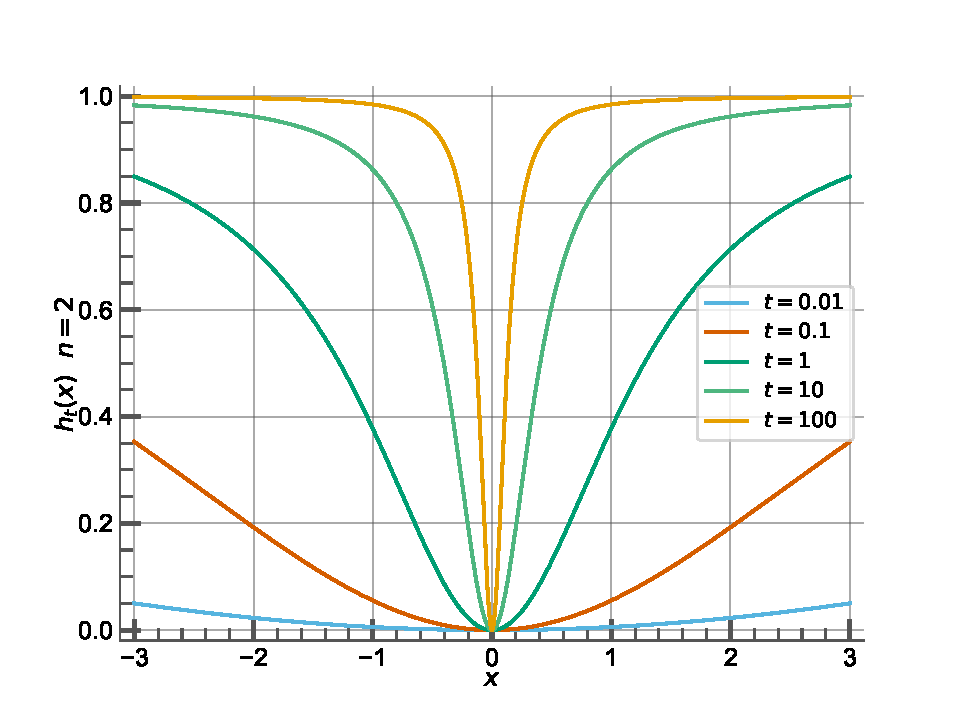
\includegraphics[width=0.49\linewidth]{chapter_1/assets/reparam_funct_varying_t.pdf}
        \label{fig:chap1:reparam_funct_varying_t}} \caption{\centering
    Reparametrization function $h_t$ with varying temperature parameter $t$ and
    power $n$. $t$ controls the width of the pit, and $n$ controls the steepness
    of the slope.}
    \label{fig:stopband}
\end{figure}

Weight distribution varies tremendously from one layer to another. In order to
match a specific budget (see \cref{sec:chap1:budget_loss}), the width of the
stopband, controlled by $t$, is tuned according to the weight distribution of
each layer. The manual setting of this parameter is non-trivial and cumbersome,
so in practice, $t$ is learned as a part of gradient descent on a layer-by-layer
basis.\\

% TODO: Ajouter amorce pour discussions sur l'initialisation de la température.
%the initial setting  $t_\text{init}$ of this temperature is shown in
%\cref{tbl:pruningperformances}.\\


Considering the aforementioned four properties of $h_t$, a simple choice of that
function is 
\begin{equation}
  \label{eqn:chap1:h_star_expression}
  h_t^*(x) = \exp\bigg\{{-\displaystyle\frac{1}{(tx)^n}}\bigg\}, ~ n\in 2\mathds{N},
\end{equation}
\noindent where $n$ controls the crispness of $h_t^*$. $n$ is not considered as
a parameter of $h_t$ (or $h_t^*$) since we use a fixed value for our
experiments, whereas $t$ is a learnt parameter and varies from one layer to
another. Although the function described in \cref{eqn:chap1:h_star_expression}
satisfies the four above properties, $h_t^*$ suffers from numerical instability
as it generates \ac{nan} outputs in most of the widely used deep learning
frameworks. Due to the way Backpropagation works, a single \ac{nan} in a weight
tensor makes the whole optimisation process for the entire network no longer
possible. We consider instead a stabilised variant with a similar behaviour, as
\cref{eqn:chap1:h_star_expression},  that still satisfies the four above
properties (see also \cref{fig:chap1:h_stable_vs_unstable}). This numerically
stable variant is  defined as 
\begin{equation}
  \label{eqn:chap1:stable_h_expression}
  h_t(x) = C_1 \biggl( \text{exp} \bigg\{-\displaystyle\frac{1}{(tx)^n +1}\bigg\} - C_2 \biggr),
\end{equation}
\noindent with $C_1=\frac{1}{1-e^{-1}}$ and $C_2 = e^{-1}$.\\

The addition of the scalar value 1 at the denominator in
\cref{eqn:chap1:stable_h_expression} is a mean to achieve numerical stability.
In equation \cref{eqn:chap1:h_star_expression}, the denominator $(tx)^n$ has the
potential to approach very small values that result in numerical instabilities,
leading to \ac{nan} outputs. The addition of 1 to the denominator makes the
function numerically stable and avoids producing \ac{nan} outputs. This solution
is favoured over adding a small value, such as an arbitrarily small
$\varepsilon$, as the latter requires careful consideration of its magnitude and
may result in either dramatic alterations to the shape of the function or
continued numerical instability if not carefully chosen. The addition of the
value 1 to the denominator provides a straightforward and sufficient mean to
stabilise the function. Constants $C_1$ and $C_2$ are introduced to compensate
for the slight alterations to the shape of the function caused by the addition
of 1 to the denominator and thus to ensure that the first property
(\cref{eqn:chap1:reparam_prop1}) is respected. Although both $h_t^*$ and $h_t$
satisfy the four properties, they do not possess the exact same shapes, as
demonstrated in figure (\ref{fig:chap1:h_stable_vs_unstable}).\\

\begin{figure}
  \centering
  \centerline{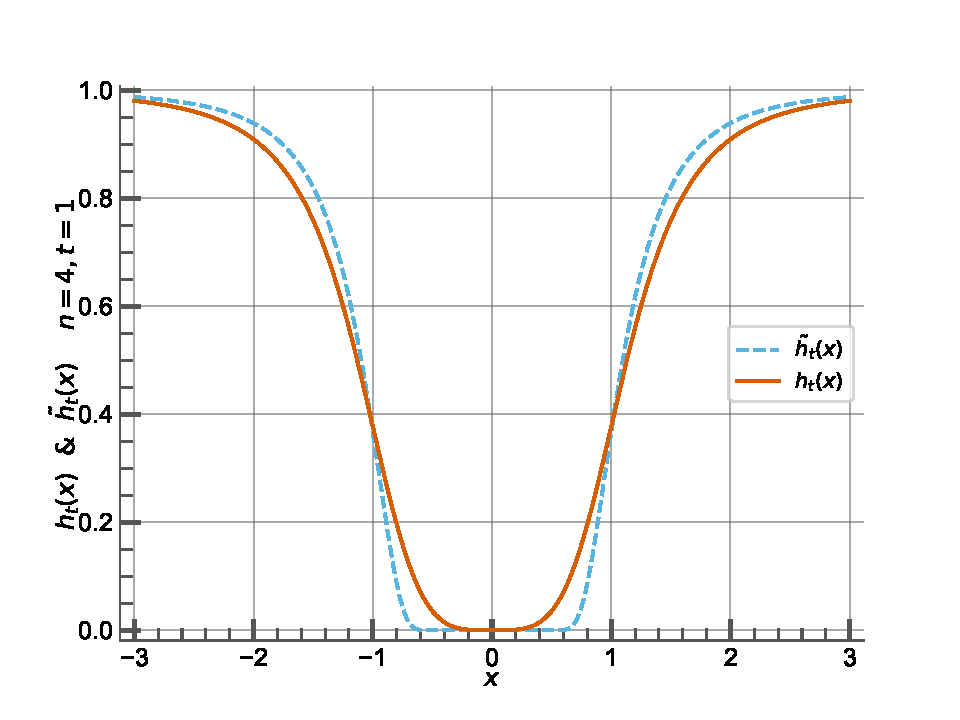
\includegraphics[width=0.49\linewidth]{chapter_1/assets/h_stable_vs_unstable.pdf}}
  \caption{\centering The unstable reparametrization function $h_t^*$ and its
  stable alternative $h_t$, with $t=1$ and $n=4$ for both functions.} 
  \label{fig:chap1:h_stable_vs_unstable}
\end{figure}

\subsection{Budget Loss}
\label{sec:chap1:budget_loss}

Most traditional pruning methods in deep learning do not explicitly incorporate
the target weight budget during the optimisation procedure. The amount of
weights pruned is typically enforced post-training, which can lead to suboptimal
results compared to methods that consider the weight budget during optimisation.
Our method introduces a budget loss term, in addition to the main task loss
term, that drives the network to match and respect a given weight budget during
the training process. Consequently, the trained network can be pruned to the
desired pruning rate with a marginal loss in accuracy and does not need
fine-tuning.\\


The considered budget is weight-based and should quantify the target fraction of
active connections in the network. To build the budget loss, we first introduce
a cost function that quantifies the number of active connections in the network.
Let $C(\{\mathbf{w}_1,\dots, \mathbf{w}_L\})$ be the {\em current} cost
associated to a neural network and its set of {\em current} weights and
$C_\text{target}$ the {\em targeted} one. $C_\text{target}$ is the number of
connections that should be active at the end of the training procedure. The
budget loss is defined as \\

\begin{equation}
  \label{eqn:chap1:simple_budget}
  {\cal L}_\text{budget} = \bigl( C(\{\mathbf{w}_1,\dots, \mathbf{w}_L\}) - C_\text{target} \bigr)^2.
\end{equation} \\


\noindent This budget loss is combined with the main task loss (a classification
loss in our experiments - see \cref{sec:chap1:experiments}). The budget loss $
{\cal L}_\text{budget}$ is in quadratic form to ensure the minimisation of this
loss will, in turn, minimise the difference between the {\em current} cost and
the {\em targeted} one. For better conditioning of this combination, we
normalise the budget loss by $C_\text{initial}$. The latter corresponds to the
cost of the primary unpruned network, which is set in practice to the number of
its parameters (see also \cref{sec:chap1:experiments}). Hence,
\cref{eqn:chap1:simple_budget} is updated as  \\

\begin{equation}
  \label{eqn:chap1:real_budget}
  {\cal L}_\text{budget} = \biggl( \displaystyle\frac{C(\{\mathbf{w}_1,\dots, \mathbf{w}_L\}) - C_\text{target}}{C_\text{initial}} \biggr)^2.
\end{equation}\\

Finally, the two losses are combined together via a strictly positive mixing
parameter $\lambda$ that  controls the relative importance of  the budget loss
${\cal L}_\text{budget}$ compared to the main task loss ${\cal L}_\text{task}$,
leading to\\

\begin{equation}
  \label{eqn:chap1:globalloss}
   {\cal L} =  {\cal L}_\text{task} + \lambda \cdot {\cal L}_\text{budget}.
\end{equation} \\

Ideally, the budget of a neural network could be evaluated as the number of
multiply-add operations, often referred to as \ac{FLOPs}, needed for a forward
pass or through the $\ell_0$ norm of its weights. However, neither are known to
be differentiable and, therefore, cannot be used in a gradient-based
optimisation. In order to circumvent this limitation, we use our weight
reparametrisation as a surrogate measure of $\ell_0$, and we define the cost
function as \\

\begin{equation}
  \label{eqn:chap1:cost_function}
  C(\{\mathbf{w}_1,\dots, \mathbf{w}_L\}) = \displaystyle \sum_{i=1}^{L} h_t(\mathbf{w}_i). 
\end{equation} \\


\begin{figure}
  \centering
  \subfloat[Number of parameters]{
      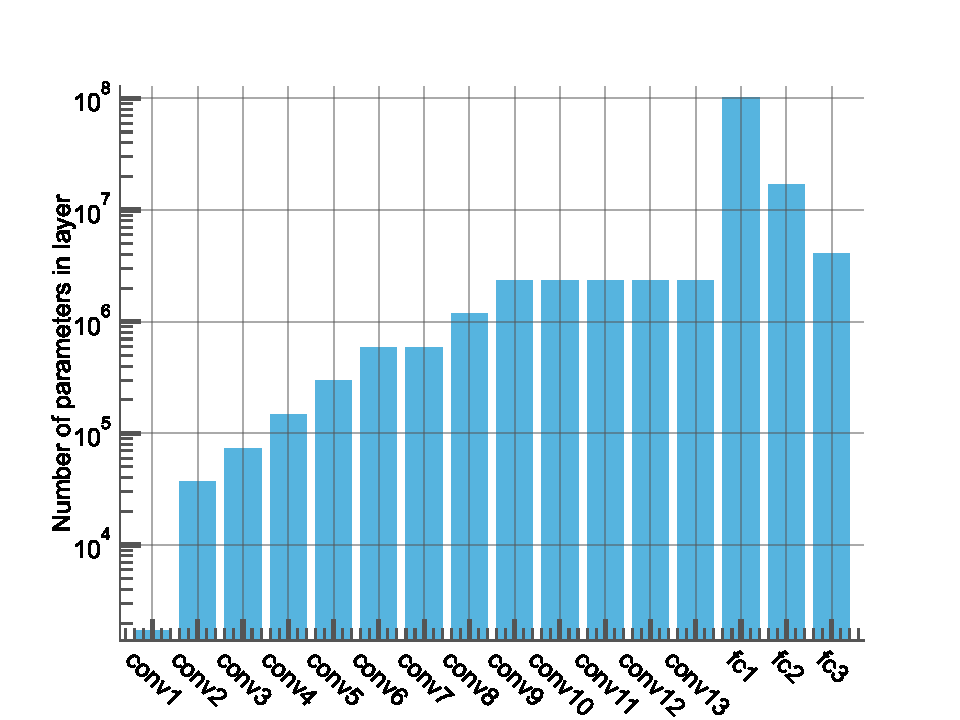
\includegraphics[width=0.49\linewidth]{chapter_1/assets/vgg16_num_params_per_layer.pdf}
      \label{fig:chap1:num_parap_vgg16}} \subfloat[Normalization factor]{
      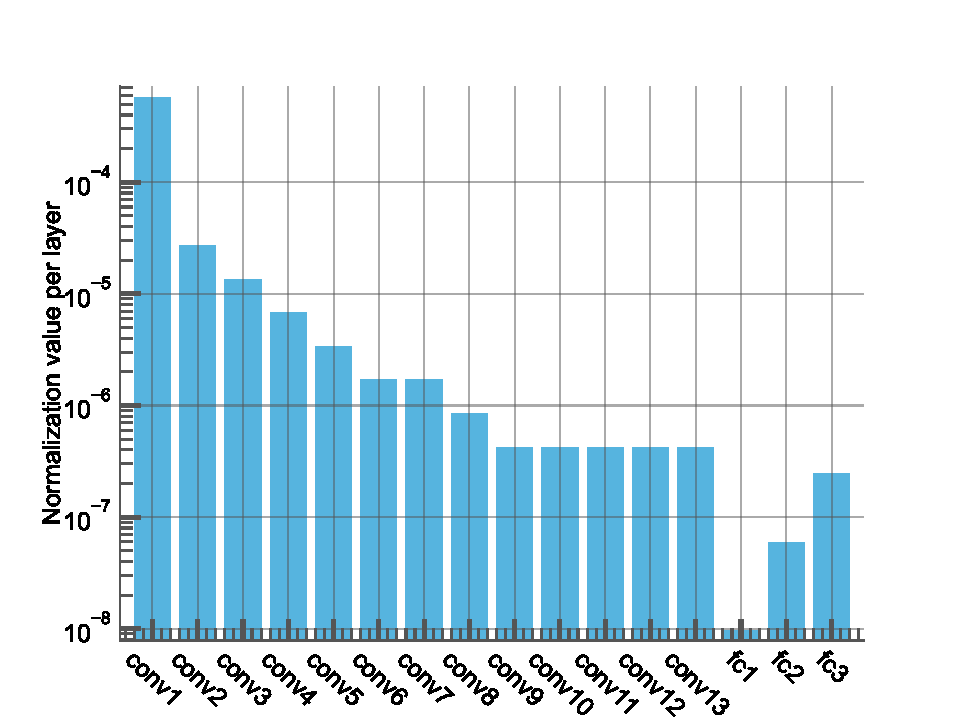
\includegraphics[width=0.49\linewidth]{chapter_1/assets/vgg16_normalization_factor_per_layer.pdf}
      \label{fig:chap1:norm_factor_vgg16}} \caption{\centering Log-scale plot of
      number of parameters and normalisation factor per layer for a VGG16
      network. The significant differences in term of the number of parameters
      yields dramatically different normalisation factors. Some of them are 4
      orders of magnitude apart, and all of them are vanishingly small compared
      to a common main task loss value.} 
  \label{fig:chap1:vgg16_per_layer_param_and_norm_factor}
\end{figure}

One could argue that the cost should be normalised layer-wise and, therefore,
that the right-hand term of \cref{eqn:chap1:cost_function} should be written as
$$\displaystyle\sum_{i=1}^{L}\frac{h_t(\mathbf{w}_i)}{\text{Card}(\mathbf{w}_i)}$$
where $\text{Card}(.)$ denotes the cardinal function, it is to say, in this
case, the number of scalar elements in a weight tensor. However, the number of
elements in a layer greatly varies from one layer to another (as demonstrated in
\cref{fig:chap1:vgg16_per_layer_param_and_norm_factor}). As a result,  the
budget loss relative importance would vary from one layer to another. More
importantly, the optimisation process would have less incentive to introduce
sparsity in larger layers since their normalisation factor would make the budget
loss negligible compared to other layers or the main task loss. This is critical
since the large layers are generally the ones where the highest pruning rates
can be achieved \cite{DBLP:journals/corr/abs-2202-12002}. Regarding the
aforementioned reasons, a better alternative is to normalise by the initial cost
$C_\text{initial}$, as done in \cref{eqn:chap1:real_budget}.\\

% endregion

\section{Experiments And Results}
\label{sec:chap1:experiments}

In this section, we will explore the effectiveness of our method on deep neural
networks for image classification. We have chosen to use three reference
databases in the field of computer vision: CIFAR10 \cite{CIFARdataset}, CIFAR100
\cite{CIFARdataset}, and TinyImageNet \cite{TinyImageNet}. We will evaluate the
impact of our method on several neural network architectures: VGG16
\cite{DBLP:journals/corr/SimonyanZ14a}, Conv4 \cite{DBLP:conf/iclr/FrankleC19},
ResNet18, and ResNet20 \cite{DBLP:conf/cvpr/HeZRS16}. This study will allow us
to demonstrate the effectiveness of our method for compressing image
classification models, as well as its influence on prediction accuracy. To that
extent, we will review the impact of both our reparametrisation and our budget
loss.\\

The CIFAR10 and CIFAR100 datasets both contain 60,000 colour images of size
32x32 pixels, split into 10 and 100 classes, respectively. The TinyImageNet
dataset is shrunk version of the ImageNet dataset
\cite{DBLP:journals/ijcv/RussakovskyDSKS15}, and contains 100,000 images of size
64x64 pixels, split into 200 classes. Each dataset is divided into two folds: a
training set and a test set. In addition to these two folds, we also use a
validation set to tune the hyperparameters of our method before testing it on
the test set. The validation dataset is obtained by selecting 10\% of the
training set. \Cref{tab:chap1:datasets} summarizes the composition of the three
datasets.\\


\begin{table}[h]
  \centering
  \begin{tabular}{lcccc}
    \toprule
    \textbf{Dataset} & \textbf{Number of images} & \textbf{Number of classes} &
    \textbf{Image size} & \textbf{Size of test set} \\ 
    \hline
    CIFAR10 & 60,000 & 10 & 32x32 & 10,000 \\ 
    CIFAR100 & 60,000 & 100 & 32x32 & 10,000\\ 
    TinyImageNet & 100,000 & 200 & 64x64 &10,000 \\ 
    \bottomrule
  \end{tabular}
  \caption{The number of images, of classes, image size and size of the test set for the three datasets used.}
  \label{tab:chap1:datasets}
\end{table}

In combination with these datasets, we use four different neural networks. Conv4
is a small and reasonably lightweight convolutional neural network which is a
shrunk-down version of the VGG16 architecture. VGG16 is a convolutional neural
of larger size and depth, which is a popular choice for image classification. We
used a slightly modified version of VGG16 that is better suited to CIFAR10. We
do not use dropout, but we use batch normalisation, and the fully connected
section has only one layer. ResNet18 is a residual neural network that
introduces skip connection in its architectural design. ResNet20 is a modified
version of the ResNet18 architecture to make it suited for CIFAR10 and CIFAR100
datasets. \Cref{tab:chap1:networks_size} summarises the size of the different
models. In our experiments, we use ResNet18 exclusively for TinyImageNet and the
other networks for CIFAR10 and CIFAR100.\\


\begin{table}[h]
  \centering
  \begin{tabular}{lllll}
  \cline{2-5}
                       & Conv4     & VGG16      & ResNet20 & ResNet18   \\ \hline
  Number of Parameters & 2,425,930 & 14,728,266 & 269,034  & 11,685,608 \\ \hline
  \end{tabular}
  \caption{\centering number of parameters for the four neural network architectures used.}
  \label{tab:chap1:networks_size}
\end{table}

\subsection{Performances}
\label{sec:chap1:performances}
Performances of our method are evaluated on CIFAR10 and CIFAR100 with Conv4,
VGG16 and ResNet20. On TinyImageNet, we evaluate our method on ResNet18. We
compare our method against magnitude pruning \cite{DBLP:conf/nips/HanPTD15}. The
key differences between our method and magnitude pruning are the following:
$(i)$ our method uses a budget loss to encourage sparsity, which takes into
account the final pruning rate from the beginning of the training process,
$(ii)$ our method does not require fine-tuning after pruning. Because of the
latter, we compare our method against magnitude pruning with and without
fine-tuning. Both methods share the following setup: networks are trained during
300 epochs with an initial learning rate of 0.1. A {\em Reduce On Plateau}
policy is applied to the learning rate: if the validation accuracy is not
improving for 10 epochs in a row, then the learning rate is decreased by a
factor of 0.3. A weight decay is applied on the weights with a penalisation
factor of $5\times10^{−5}$. An Early Stopping policy was used to stop the
training prematurely if no improvement of the test accuracy is observed in 60
epochs. To keep the comparison fair, for magnitude pruning, the 300 epochs are
split into two phases: the first 150 epochs are dedicated to the training of the
network, and the last 150 epochs are used for fine-tuning the pruned network. In
the fine-tuning phase, the learning rate is divided by 100 for better
convergence. \\

Results are repported on
\cref{fig:chap1:reparam_vs_mpft_conv4,fig:chap1:reparam_vs_mpft_resnet20,fig:chap1:reparam_vs_mpft_vgg16}.
In the figures mentioned above, our method (denoted \emph{Ours}) is compared to
magnitude pruning with and without fine-tuning (denoted \emph{MP w/ FT} and
\emph{MP w/o FT}, respectively). All three methods are evaluated on the test
fold of the dataset once the network has been pruned up to the pruning rate
indicated on the \emph{x-axis}. The test accuracy is reported on the
\emph{y-axis} as a float between 0 and 1 (0 being all images wrongly classified
and 1 being all images correctly classified). Each solid line representing a
method is the mean of 5 independent runs. The coloured area surrounding the
solid line represents the range within plus or minus one standard deviation. In
addition to the three methods, the dashed lines represent the performances of an
unpruned network trained without weight reparametrisation and budget loss
(denoted \emph{baseline}) and the accuracy of our method before the effective
pruning (denoted \emph{Ours (pre pruning)}). Sub-figures (c) and (d) of
\cref{fig:chap1:reparam_vs_mpft_conv4,fig:chap1:reparam_vs_mpft_resnet20,fig:chap1:reparam_vs_mpft_vgg16}.
represents the number of epochs (\emph{y-axis}) needed to obtain the best model
for each method, depending on the pruning rate (\emph{x-axis}).\\


Overall, our method performs consistently better than magnitude pruning without
fine-tuning (\emph{MP w/o FT}) and, for almost all pruning rates, better than
magnitude pruning with fine-tuning (\emph{MP w/ FT}) on the CIFAR10 and CIFAR100
datasets. In particular, our method significantly outperforms magnitude pruning
in both setups (with and without fine-tuning) for Conv4 networks (cf.
\cref{fig:chap1:reparam_vs_mpft_conv4_cifar10}). For the VGG16 network, we
observe the same trend, although the difference is less significant. For
ResNet20, magnitude pruning slightly overperforms our method on CIFAR100 for
high pruning rates (more than 90\%).
\Cref{fig:chap1:reparam_vs_mpft_conv4_cifar10_epochs,fig:chap1:reparam_vs_mpft_conv4_cifar100_epochs,fig:chap1:reparam_vs_mpft_vgg16_cifar10_epochs,fig:chap1:reparam_vs_mpft_vgg16_cifar100_epochs,fig:chap1:reparam_vs_mpft_resnet20_cifar10_epochs,fig:chap1:reparam_vs_mpft_resnet20_cifar100_epochs}
show that our method requires an equivalent number of epochs compared to
magnitude pruning for a higher level of performance (i.e. a higher test
accuracy). Magnitude pruning requires fewer epochs than our method, only at high
pruning rates (more than 90\%). On TinyImageNet
(\cref{fig:chap1:reparam_vs_mpft_resnet18}), our method outperforms magnitude
pruning with and without fine-tuning up until very high pruning rates (95\%). In
any cases
(\cref{fig:chap1:reparam_vs_mpft_conv4,fig:chap1:reparam_vs_mpft_vgg16,fig:chap1:reparam_vs_mpft_resnet20,fig:chap1:reparam_vs_mpft_resnet18}),
Our method produces much more stable results, and variations from one run to
another are significantly slimmer than the ones in magnitude pruning. Indeed,
the combination of the reparametrisation and the budget loss act, on the one
hand, as a regulariser and, on the other hand, helps to prepare the network for
the effective pruning step.\\

% region: perfs_figures
\begin{figure}
  \centering
  \subfloat[Conv4 - CIFAR10]{
      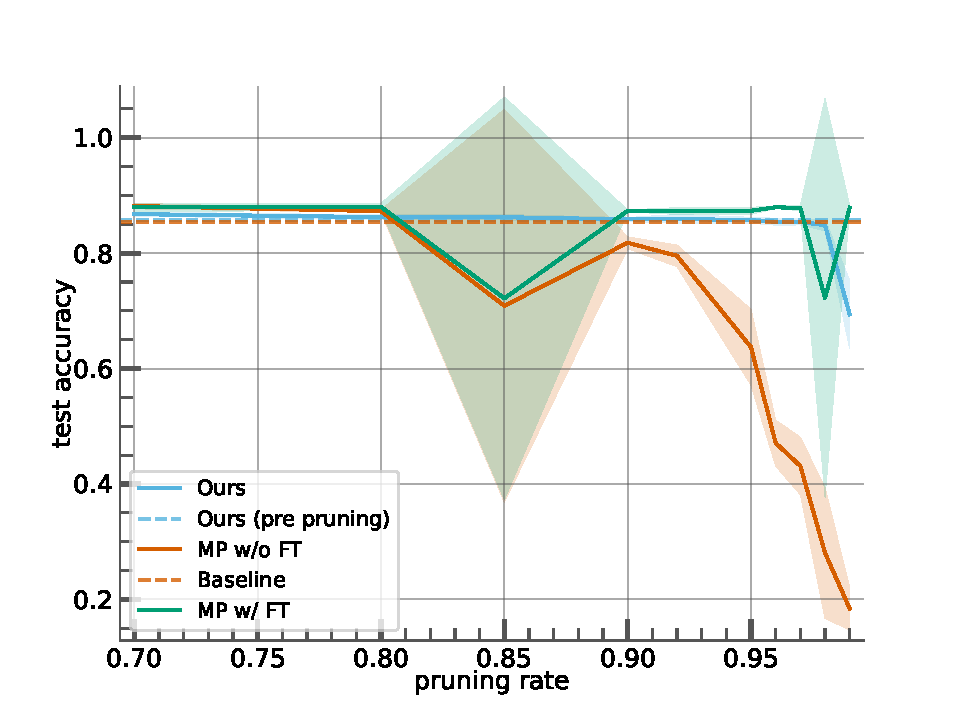
\includegraphics[width=0.49\linewidth]{chapter_1/assets/reparam_vs_mpft_Conv4_cifar10.pdf}
      \label{fig:chap1:reparam_vs_mpft_conv4_cifar10}}
  \subfloat[Conv4 - CIFAR100]{
      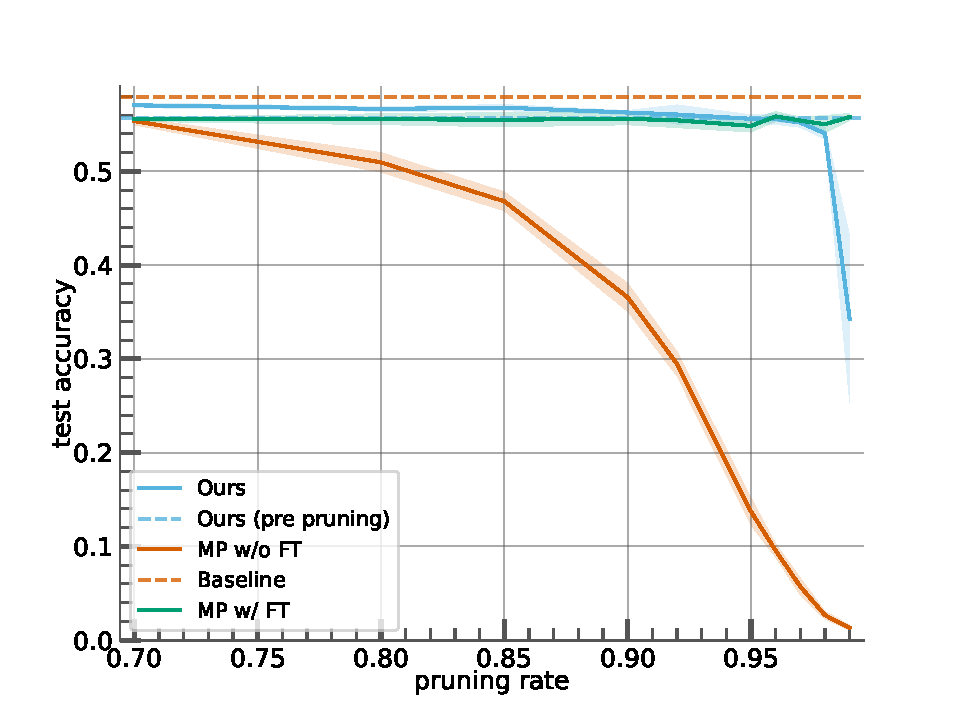
\includegraphics[width=0.49\linewidth]{chapter_1/assets/reparam_vs_mpft_Conv4_cifar100.pdf}
      \label{fig:chap1:reparam_vs_mpft_conv4_cifar100}}
      \\
  \subfloat[Conv4 - CIFAR10 (Number of Epochs)\label{fig:chap1:reparam_vs_mpft_conv4_cifar10_epochs}]{
      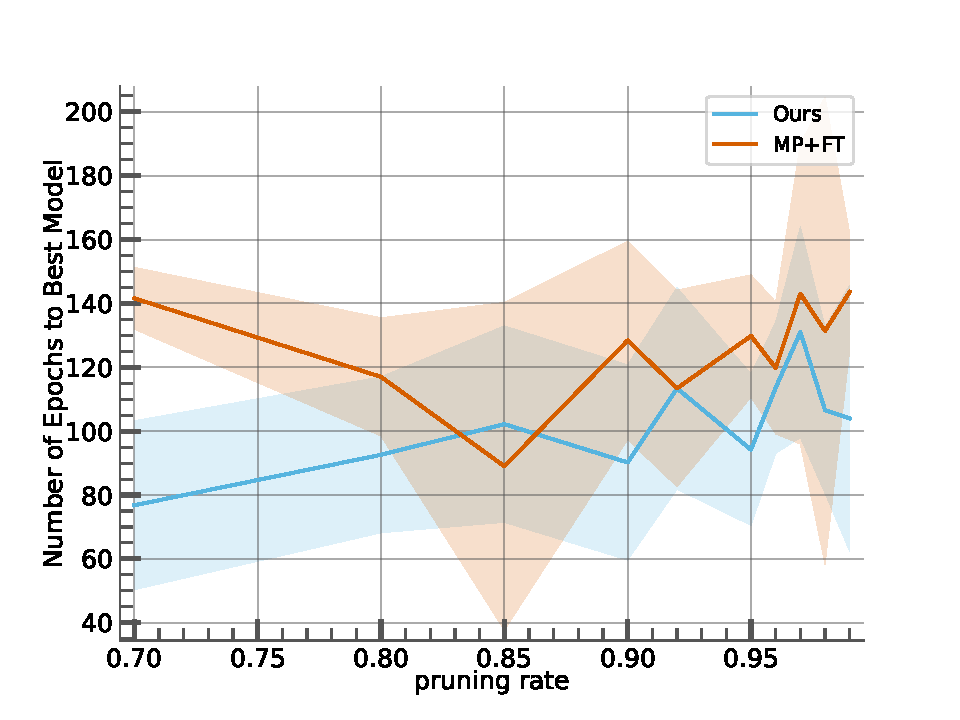
\includegraphics[width=0.49\linewidth]{chapter_1/assets/reparam_vs_mpft_training_time_Conv4_cifar10.pdf}}
  \subfloat[Conv4 - CIFAR100 (Number of Epochs)\label{fig:chap1:reparam_vs_mpft_conv4_cifar100_epochs}]{
      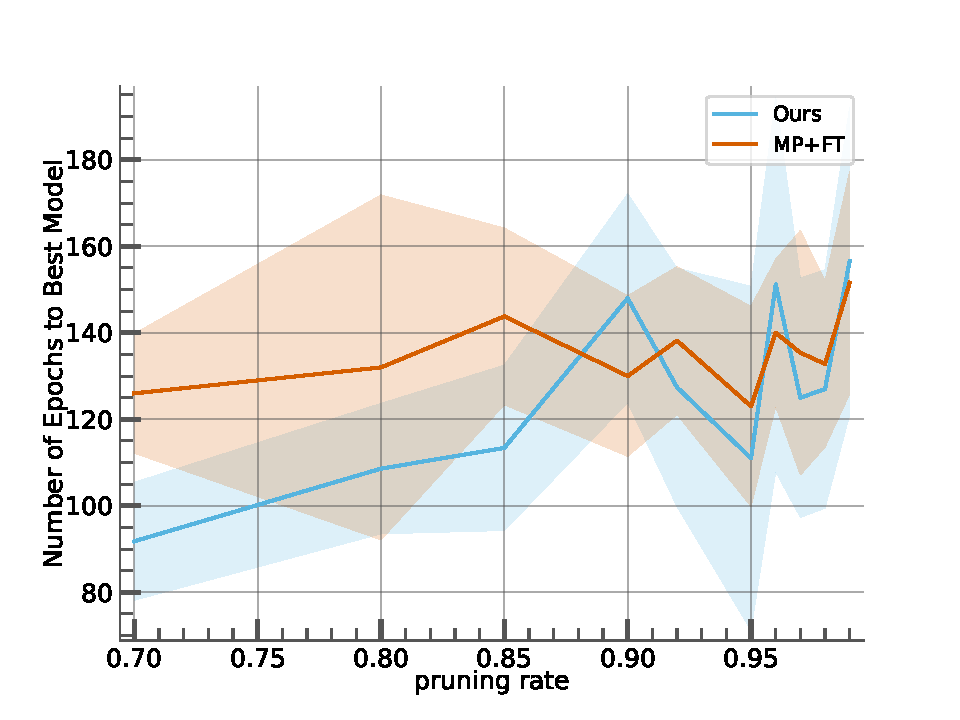
\includegraphics[width=0.49\linewidth]{chapter_1/assets/reparam_vs_mpft_training_time_Conv4_cifar100.pdf}}
  \caption{\centering Performances comparison of our method {\em(Ours)} against
  magnitude pruning without {\em(MP w/o FT)} and with fine-tuning {\em(MP w/ FT)} with a Conv4 network on
  CIFAR10 and CIFAR100 datasets, for different pruning rates.
  \Cref{fig:chap1:reparam_vs_mpft_conv4_cifar10} and
  \cref{fig:chap1:reparam_vs_mpft_conv4_cifar100} show the testing accuracy of
  the model and \cref{fig:chap1:reparam_vs_mpft_conv4_cifar10_epochs} and
  \cref{fig:chap1:reparam_vs_mpft_conv4_cifar100_epochs} the number of epochs
  needed to obtain the best model.}
  \label{fig:chap1:reparam_vs_mpft_conv4}
\end{figure}

\begin{figure}
  \centering
  \subfloat[VGG16 - CIFAR10]{
      \includegraphics[width=0.49\linewidth]{chapter_1/assets/reparam_vs_mpft_PrunableVGG16_cifar10.pdf}
      \label{fig:chap1:reparam_vs_mpft_vgg16_cifar10}} 
  \subfloat[VGG16 - CIFAR100]{
      \includegraphics[width=0.49\linewidth]{chapter_1/assets/reparam_vs_mpft_PrunableVGG16_cifar100.pdf}
      \label{fig:chap1:reparam_vs_mpft_vgg16_cifar100}} 
  \\
  \subfloat[VGG16 - CIFAR10 (Number of Epochs)\label{fig:chap1:reparam_vs_mpft_vgg16_cifar10_epochs}]{
    \includegraphics[width=0.49\linewidth]{chapter_1/assets/reparam_vs_mpft_training_time_PrunableVGG16_cifar10.pdf}}
  \subfloat[VGG16 - CIFAR100 (Number of Epochs)\label{fig:chap1:reparam_vs_mpft_vgg16_cifar100_epochs}]{
      \includegraphics[width=0.49\linewidth]{chapter_1/assets/reparam_vs_mpft_training_time_PrunableVGG16_cifar100.pdf}}

    
  \caption{\centering Performances comparison of our method \em{(Ours)} against
  magnitude pruning with fine-tuning \em{(MP+FT)} with a VGG16 network on
  CIFAR10 and CIFAR100 datasets, for different pruning rates.
  \Cref{fig:chap1:reparam_vs_mpft_vgg16_cifar10} and
  \cref{fig:chap1:reparam_vs_mpft_vgg16_cifar100} show the testing accuracy of
  the model and \cref{fig:chap1:reparam_vs_mpft_vgg16_cifar10_epochs} and
  \cref{fig:chap1:reparam_vs_mpft_vgg16_cifar100_epochs} the
  number of epochs needed to obtain the best model.}
  \label{fig:chap1:reparam_vs_mpft_vgg16}
\end{figure}

\begin{figure}
  \centering
  \subfloat[ResNet20 - CIFAR10\label{fig:chap1:reparam_vs_mpft_resnet20_cifar10}]{
      \includegraphics[width=0.49\linewidth]{chapter_1/assets/reparam_vs_mpft_PrunableResNet20_cifar10.pdf}}
  \subfloat[ResNet20 - CIFAR100\label{fig:chap1:reparam_vs_mpft_resnet20_cifar100}]{
      \includegraphics[width=0.49\linewidth]{chapter_1/assets/reparam_vs_mpft_PrunableResNet20_cifar100.pdf}} 
  \\
  \subfloat[ResNet20 - CIFAR10 (Number of Epochs)\label{fig:chap1:reparam_vs_mpft_resnet20_cifar10_epochs}  ]{
      \includegraphics[width=0.49\linewidth]{chapter_1/assets/reparam_vs_mpft_training_time_PrunableResNet20_cifar10.pdf}}
  \subfloat[ResNet20 - CIFAR100 (Number of Epochs)\label{fig:chap1:reparam_vs_mpft_resnet20_cifar100_epochs}]{
      \includegraphics[width=0.49\linewidth]{chapter_1/assets/reparam_vs_mpft_training_time_PrunableResNet20_cifar100.pdf}}
  \caption{\centering Performances comparison of our method \em{(Ours)} against
  magnitude pruning with fine-tuning \em{(MP+FT)} with a ResNet20 network on
  CIFAR10 and CIFAR100 datasets, for different pruning rates.
  \Cref{fig:chap1:reparam_vs_mpft_resnet20_cifar10} and
  \cref{fig:chap1:reparam_vs_mpft_resnet20_cifar100} show the
  testing accuracy of the model and
  \cref{fig:chap1:reparam_vs_mpft_resnet20_cifar10_epochs} and
  \cref{fig:chap1:reparam_vs_mpft_resnet20_cifar100_epochs}
  the number of epochs needed to obtain the best model.}
  \label{fig:chap1:reparam_vs_mpft_resnet20}
\end{figure}


\begin{figure}
  \centering
  \includegraphics[width=0.49\textwidth]{chapter_1/assets/reparam_vs_mpft_PrunableResNet18_tinyimagenet.pdf}
  \caption{Performances comparison of our method \em{(Ours)} against
  magnitude pruning with fine-tuning \em{(MP+FT)} with a ResNet18 network on
  TinyImageNet dataset, for different pruning rates.}
  \label{fig:chap1:reparam_vs_mpft_resnet18}
\end{figure}

% endregion: perfs_figures

\subsection{Optimal value of \texorpdfstring{$\lambda$}{Lambda}}
\label{sec:chap1:impact_of_lambda}
Our method relies on a budget loss which relative importance compared to the
main task loss is controlled by a parameter $\lambda$ (cf.
\cref{eqn:chap1:globalloss}). The choice of this parameter is crucial to ensure
a good tradeoff between \emph{(i)} the respect of the budget, in order to
mitigate the performance drop following the effective pruning step; and
\emph{(ii)} the optimisation of the main task loss, which influences the final
performance. The achieved budget as a function of the parameter $\lambda$ is
detailed for different pruning rates in
\cref{fig:chap1:lambda_impact_pruning_90,fig:chap1:lambda_impact_pruning_95,fig:chap1:lambda_impact_pruning_99}.
In these figures, the achieved budget is computed as the sum of the weights reparametrization\\

For low pruning rates (cf. \cref{fig:chap1:lambda_impact_pruning_90}), a low
value of lambda does not enforce the respect of the budget and in this case, the
final network has a smaller achieved budget than the targeted one. Similarly,
for higher pruning rates (cf. \cref{fig:chap1:lambda_impact_pruning_99}), a low
value of lambda results in a budget in excess compared to the targeted one. In
both cases, the performances of networks trained with a low value of $\lambda$
are subpar compared to higher values, as reported in
\cref{tab:chap1:lambda_impact}. On the opposite of the spectrum, high values of
$\lambda$ lay too much emphasis on the budget loss, and the network performances
are negatively impacted. Following the abovementioned considerations, we set the
value of $\lambda$ to 5 for all the experiments. This value strikes the best
balance between the two objectives: budget loss and main task loss.

% region: lambda_impact_figures

\begin{figure}
  \centering
  \subfloat[Pruning 90\% of the weights\label{fig:chap1:lambda_impact_pruning_90}]{
    \includegraphics[width=0.49\linewidth]{chapter_1/assets/lambda_impact_pr_90_C4_CIFAR10.pdf}}
  \subfloat[Pruning 95\% of the weights\label{fig:chap1:lambda_impact_pruning_95}]{
    \includegraphics[width=0.49\linewidth]{chapter_1/assets/lambda_impact_pr_95_C4_CIFAR10.pdf}}
  \\
  \subfloat[Pruning 99\% of the weights\label{fig:chap1:lambda_impact_pruning_99}]{
    \includegraphics[width=0.49\linewidth]{chapter_1/assets/lambda_impact_pr_99_C4_CIFAR10.pdf}}
    \caption{\centering Impact of the parameter $\lambda$ on the achieved final
    budget for a Conv4 network on CIFAR10 dataset, for various pruning rates. A
    too-small value of $\lambda$ does not make the actual budget match the desired
    budget. The actual budget is either too small
    (\cref{fig:chap1:lambda_impact_pruning_90}) or too high
    (\cref{fig:chap1:lambda_impact_pruning_99}) compared to the target, depending
    on the applied pruning rate.}
  \label{fig:chap1:lambda_impact}
  \end{figure}  


\begin{table}[tbp]
  \centering
  \begin{center}
    \begin{tabular}{llcc}
      \toprule
      Pruning Rate & $\lambda$ & Achieved Budget & Test Accuracy (post pruning) \\
      \midrule
      \multirow{4}{*}{0.9} & 0.005 & 5.25 $\pm$ 0.69 & 85.83 $\pm$ 0.83 \\
      & 0.5 & 8.06 $\pm$ 0.19 & 86.34 $\pm$ 0.64 \\
      & 5 & 9.93 $\pm$ 0.03 & 85.82 $\pm$ 0.74 \\
      & 50 & \textbf{10.00 $\pm$ 0.01} & \textbf{86.52 $\pm$ 0.46} \\
      \midrule
      \multirow{4}{*}{0.95} & 0.005 & 5.22 $\pm$ 0.73 & \textbf{86.27 $\pm$ 0.32} \\
      & 0.5 & 4.33 $\pm$ 0.41 & 85.66 $\pm$ 0.74 \\
      & 5 & 4.85 $\pm$ 0.19 & 86.11 $\pm$ 0.48 \\
      & 50 & \textbf{5.03 $\pm$ 0.02} & 85.37 $\pm$ 0.37 \\
      \midrule
      \multirow{4}{*}{0.99} & 0.005 & 4.60 $\pm$ 0.29 & 40.52 $\pm$ 5.27 \\
      & 0.5 & 3.69 $\pm$ 0.38 & 42.45 $\pm$ 9.02 \\
      & 5 & 1.89 $\pm$ 0.45 & \textbf{76.85 $\pm$ 6.34} \\
      & 50 & \textbf{2.09 $\pm$ 0.15} & 10.00 $\pm$ 0.00 \\
      \bottomrule
    \end{tabular}
  \end{center}
  \caption{\centering
    Impact of the parameter $\lambda$ on the achieved budget and the post-pruning test accuracy of the model for a Conv4 network on the CIFAR10 dataset
    for various pruning rates. Although a high value of $\lambda$ ensures 
    the target budget is reached, it also leads to a lower test accuracy when
    the pruning rate increases.}
    \label{tab:chap1:lambda_impact}
\end{table}

% endregion: lambda_impact_figures

\subsection{Impact of the budget loss}
\label{sec:chap1:impact_of_budget_loss}
To establish the importance and the efficacy of the budget loss in our method,
we present in this section the results of a comparative experimental analysis
with alternative variants.  Specifically, we investigated the impact of the
budget loss by comparing it with two other variants: \emph{(i)} a variant where the
budget loss was removed, and \emph{(ii)} a variant where the budget loss is replaced
with an $L_1$ regularization loss on the network weights. To remove the budget
loss, the value of $\lambda$ is set to zero 0 in \cref{eqn:chap1:globalloss}. In the
second variant, we varied the mixing coefficient $\lambda$ between 0.1 and 100.
Considering the same issue of loss conditioning as in
\cref{sec:chap1:budget_loss}, the $L_1$ loss is divided by the total number of
parameters before being added to the global loss. The new global loss is
expressed as :

\begin{equation}
  \label{eqn:chap1:globalloss_l1}
  \mathcal{L} = \mathcal{L}_{task} + \lambda \cdot \frac{1}{N} \sum_{i=1}^{N} \left| w_i \right|
\end{equation}

Where $|~.~|$ represents the absolute value, and $N$ is the total number of
parameters in the network (as reported in \cref{tab:chap1:networks_size}).\\

In both variants, the reparametrisation is kept in order to isolate the impact
of the budget loss. We evaluated the performance of our approach and the two
variants on the CIFAR10 and CIFAR100 datasets using Conv4, VGG16, and ResNet20
networks. The results are presented in
\cref{fig:chap1:no_budget_conv4,fig:chap1:no_budget_resnet20,fig:chap1:no_budget_vgg16}.
In the figures mentioned above, the variant without the budget loss is denoted
\emph{w/o budget}, and the variant with a $L_1$ regularisation loss is referred
as \emph{$L_1$ reg.}. The results denoted \emph{w/ budget} represents our method
in the same setup as in \cref{sec:chap1:performances}.\\

Removing the budget loss (variant \emph{(i)}) negatively impacts the network
performances. The test accuracy is systematically lower than the one obtained
with the budget loss. This is particularly visible in
\cref{fig:chap1:no_budget_conv4_cifar100,fig:chap1:no_budget_vgg16_cifar100}.
Removing the budget loss does not allow to introduce sparsity, much less to
respect a target budget. Therefore, effective pruning impacts all the more
negatively the network performance since it was not trained with a prior on
neither sparsity nor budget. \\

Replacing the budget loss with a $L_1$ regularisation loss (variant \emph{(ii)})
also impacts negatively the performance, with the exception of the ResNet20
network (\cref{fig:chap1:no_budget_resnet20}). Although the performance are
generally worse than our method (\emph{w/ budget}), results idicate that the
mixing coefficient $\lambda$ has a major importance. Indeed, the $L_1$
regulatisation does not target a precise budget, however, it still introduces
sparsity in the network. Thus, for certain pruning rates, the variant
\emph{(ii)} can exhibit better results than our method (especially visible on
\cref{fig:chap1:no_budget_resnet20_cifar10,fig:chap1:no_budget_resnet20_cifar100}).
Nevertheless, the choice of $\lambda$ is critial and not trivial. Because of the
absence of a budget loss, the level of sparsity is to be controlled only by the
parameter $\lambda$, which makes it difficult to find a single value suited for
a large range of pruning rates, networks and datasets.\\

In contrast, our method is able to achieve good performance accross multiple and
diverse conditions, without the need to fine-tune the value of $\lambda$.
Experiments presented in this section reveal that the budget loss is a critical
component of the method to train networks and prune them, while introducing a
minimal impact on the performance if no fine-tuning is applied. While the $L_1$
regularization loss may achieve superior performance in certain cases, our
method is more straightforward and robust in its applicability across various
scenarios.\\

% region: no budget
\begin{figure}
  \centering
  \subfloat[Conv4 CIFAR10\label{fig:chap1:no_budget_conv4_cifar10}]{
    \includegraphics[width=0.49\textwidth]{chapter_1/assets/ours_vs_no_lambda_vs_l1_only_cifar10_Conv4.pdf}}
    \subfloat[Conv4 CIFAR100\label{fig:chap1:no_budget_conv4_cifar100}]{
    \includegraphics[width=0.49\textwidth]{chapter_1/assets/ours_vs_no_lambda_vs_l1_only_cifar100_Conv4.pdf}}
    \caption{\centering Comparison of our method and its vairant without the
    budget loss. The experimental reults are denoted \emph{$L_1$ reg.}, wherein
    the budget loss is replaced by a $L_1$ regularisation loss on the network
    weights. The mixing coefficient $\lambda$ is varied from 0.1 to 100,
    depending on the experiment. \emph{w/o budget} denotes the asbcence of the
    budget loss (this is equivalent to $\lambda = 0$). On the other hand,
    \emph{w/ budget} corresponds to our method, with the same setup as described
    in \cref{sec:chap1:performances}. Results are presented for a Conv4 network,
    trained on CIFAR10 (\cref{fig:chap1:no_budget_conv4_cifar10}) and CIFAR100
    (\cref{fig:chap1:no_budget_conv4_cifar100})} 
      \label{fig:chap1:no_budget_conv4}
\end{figure}
  
  

\begin{figure}
  \centering
  \subfloat[ResNet20 CIFAR10\label{fig:chap1:no_budget_resnet20_cifar10}]{
    \includegraphics[width=0.49\textwidth]{chapter_1/assets/ours_vs_no_lambda_vs_l1_only_cifar10_PrunableResNet20.pdf}}
    \subfloat[ResNet20 CIFAR100\label{fig:chap1:no_budget_resnet20_cifar100}]{
    \includegraphics[width=0.49\textwidth]{chapter_1/assets/ours_vs_no_lambda_vs_l1_only_cifar100_PrunableResNet20.pdf}}
    \caption{\centering Comparison of our method and its vairant without the
    budget loss. The experimental reults are denoted \emph{$L_1$ reg.}, wherein
    the budget loss is replaced by a $L_1$ regularisation loss on the network
    weights. The mixing coefficient $\lambda$ is varied from 0.1 to 100,
    depending on the experiment. \emph{w/o budget} denotes the asbcence of the
    budget loss (this is equivalent to $\lambda = 0$). On the other hand,
    \emph{w/ budget} corresponds to our method, with the same setup as described
    in \cref{sec:chap1:performances}. Results are presented for a ResNet20
    network, trained on CIFAR10 (\cref{fig:chap1:no_budget_resnet20_cifar10})
    and CIFAR100 (\cref{fig:chap1:no_budget_resnet20_cifar100})}       
    \label{fig:chap1:no_budget_resnet20}
\end{figure}
  
    

\begin{figure}
  \centering
  \subfloat[VGG16 CIFAR10\label{fig:chap1:no_budget_vgg16_cifar10}]{
    \includegraphics[width=0.49\textwidth]{chapter_1/assets/ours_vs_no_lambda_vs_l1_only_cifar10_PrunableVGG16.pdf}}
    \subfloat[VGG16 CIFAR100\label{fig:chap1:no_budget_vgg16_cifar100}]{
    \includegraphics[width=0.49\textwidth]{chapter_1/assets/ours_vs_no_lambda_vs_l1_only_cifar100_PrunableVGG16.pdf}}
    \caption{\centering Comparison of our method and its vairant without the
    budget loss. The experimental reults are denoted \emph{$L_1$ reg.}, wherein
    the budget loss is replaced by a $L_1$ regularisation loss on the network
    weights. The mixing coefficient $\lambda$ is varied from 0.1 to 100,
    depending on the experiment. \emph{w/o budget} denotes the asbcence of the
    budget loss (this is equivalent to $\lambda = 0$). On the other hand,
    \emph{w/ budget} corresponds to our method, with the same setup as described
    in \cref{sec:chap1:performances}. Results are presented for a VGG16 network,
    trained on CIFAR10 (\cref{fig:chap1:no_budget_vgg16_cifar10}) and CIFAR100
    (\cref{fig:chap1:no_budget_vgg16_cifar100})}       
    \label{fig:chap1:no_budget_vgg16}
\end{figure}

% endregion: no budget

% \subsection{Impact of the reparametrization}
% \label{sec:chap1:impact_of_reparametrization}

\subsection{Fine tuning context}
\label{sec:chap1:impact_of_fine_tuning}

Although the method presented in this chapter was designed from the ground up to
circumvent the need for fine-tuning, it can be used to fine-tune a network
trained conventionally. In this section, we compare the performances of a
network trained in a standard way, pruned and then fine-tuned with two methods:
Our method and standard fine-tuning \cite{DBLP:conf/nips/HanPTD15}. This setup
is evaluated on Conv4, ResNet20 and VGG16 for both CIFAR10 and CIFAR100. The
results are shown in 
\cref{fig:chap1:finetuning_impact_conv4,fig:chap1:finetuning_impact_resnet20,fig:chap1:finetuning_impact_vgg6}.
First, a network is trained for 150 epochs on the main classification task. Then
it is pruned up to a specified pruning rate. The pruning criterion used is the
magnitude of the weights where weights with the smallest absolute value are
removed in an unstructured way. The pruned network is then fine-tuned for 300
epochs with an early stopping criterion based on the validation accuracy. The
training is stopped prematurely if the validation accuracy does not improve for
30 epochs. \\

Except for results with the Conv4 networks, fine-tuning a network with our
method overperforms the conventional fine-tuning method by a comfortable margin
on ResNet20 across all pruning rates (\cref{fig:chap1:finetuning_impact_resnet20}) and VGG16
(\cref{fig:chap1:finetuning_impact_vgg6}) for pruning rates higher than 96\%.
Moreover, the networks produced by fine-tuning with our method are much more
consistent from one run to another. This is illustrated by the standard
deviation being so small that the colored area around the solid line is barely
visible on the graphs. This is not the case for the conventional fine-tuning
where performances vary greatly from one run to another. This is especially
visible on \cref{fig:chap1:finetuning_impact_conv4_cifar10}. 

% region: fine-tuning

\begin{figure}
\centering
\subfloat[Conv4 CIFAR10\label{fig:chap1:finetuning_impact_conv4_cifar10}]{
  \includegraphics[width=0.49\textwidth]{chapter_1/assets/finetuning_cifar10_Conv4.pdf}}
  \subfloat[Conv4 CIFAR100\label{fig:chap1:finetuning_impact_conv4_cifar100}]{
  \includegraphics[width=0.49\textwidth]{chapter_1/assets/finetuning_cifar100_Conv4.pdf}}
  \caption{\centering Fine-tuning of a Conv4 network pruned by magnitude pruning
  (\emph{MP w/o FT}) on the CIFAR10 and CIFAR100 datasets for various pruning
  rates. Conventional (\emph{MP w/ FT}) fine-tuning is compared to fine-tuning
  with our method (\emph{pruned+FT (w/ our method)}). Our method is shown for
  comparison purposes (\emph{Ours}). On this network, our method performs better
  than other approaches. Fine-tuning the network with our method provides better
  results than fine-tuning it with a conventional method.}
    \label{fig:chap1:finetuning_impact_conv4}
\end{figure}


\begin{figure}
\centering
\subfloat[ResNet20 CIFAR10\label{fig:chap1:finetuning_impact_resnet20_cifar10}]{
  \includegraphics[width=0.49\textwidth]{chapter_1/assets/finetuning_cifar10_PrunableResNet20.pdf}}
  \subfloat[ResNet20 CIFAR100\label{fig:chap1:finetuning_impact_resnet20_cifar100}]{
  \includegraphics[width=0.49\textwidth]{chapter_1/assets/finetuning_cifar100_PrunableResNet20.pdf}}
  \caption{\centering Fine-tuning of a ResNet20 network pruned by magnitude
  pruning (\emph{MP w/o FT}) on the CIFAR10 and CIFAR100 datasets with various
  pruning rates. r  Conventional (\emph{MP w/ FT}) fine-tuning is compared to
  fine-tuning with our method (\emph{pruned+FT (w/ our method)}). Our method is
  shown for comparison purposes (\emph{Ours}). On this network, fine-tuning with
  our method considerably overperforms other approaches.}
    \label{fig:chap1:finetuning_impact_resnet20}
\end{figure}


\begin{figure}
\centering
\subfloat[VGG16 CIFAR10\label{fig:chap1:finetuning_impact_vgg16_cifar10}]{
  \includegraphics[width=0.49\textwidth]{chapter_1/assets/finetuning_cifar10_PrunableVGG16.pdf}}
  \subfloat[VGG16 CIFAR100\label{fig:chap1:finetuning_impact_vgg16_cifar100}]{
  \includegraphics[width=0.49\textwidth]{chapter_1/assets/finetuning_cifar100_PrunableVGG16.pdf}}
  \caption{\centering Fine-tuning of a ResNet20 network pruned by magnitude
  pruning (\emph{MP w/o FT}) on the CIFAR10 and CIFAR100 datasets with various
  pruning rates. r  Conventional (\emph{MP w/ FT}) fine-tuning is compared to
  fine-tuning with our method (\emph{pruned+FT (w/ our method)}). Our method is
  shown for comparison purposes (\emph{Ours}). On this network, fine-tuning with
  our method performs on par with other methods up to 95\% of pruning. For
  higher pruning rates, it other performs other approaches.}
    \label{fig:chap1:finetuning_impact_vgg6}
\end{figure}

% endregion: fine-tuning




\section{Conclusion and perspectives}

\chapter{Mask Training}
\label{chap:chapter2}


\localtableofcontents


\begin{abstract}

  This chapter focuses on the development of lightweight and efficient neural
  networks for image classification tasks, particularly in visual category
  recognition. These lightweight networks are increasingly important for
  intelligent embedded systems with limited computational resources and energy
  availability. Pruning techniques are popular in designing lightweight
  networks, but they require weight training, pruning and fine-tuning. These
  weights are pruned based on criteria or saliency indicators that are learned
  alongside the weights.
  
  This chapter introduces approaches that extract effective subnetworks by
  pruning large untrained networks, without weight training. A new method, named
  \acf{ASLP}, is proposed to extract effective subnetworks from a large,
  untrained deep neural network using the \acf{STGS} technique, which enables
  stochastic computation graphs to be trained with discrete variables while
  still preserving differentiability. Additionally, the \acf{SR} weight
  rescaling mechanism is introduced. It rescales the weight distributions of the
  selected subnetworks and as a result, improves the performance and reduces the
  number of epochs required for training as shown in later experiments. Finally,
  we introduce a novel pruning strategy that finds the pruning rate yielding the
  best performances, without the need to search for and enforce a fixed pruning
  rate.\\

  The \ac{ASLP} method, which integrates the \ac{STGS} sampling technique and the
  \ac{SR} mechanism, is evaluated through experiments on CIFAR-10, CIFAR-100,
  and TinyImageNet datasets. In most cases, \ac{ASLP} outperforms other
  state-of-the-art methods and consistently surpasses them for various network
  architectures. Further experiments show that the sparsity of the networks
  extracted with \ac{ASLP} can be increased with minimal impact on the
  performance. They also demonstrate the robustness of the method to extreme
  learning rate values and the effectiveness of the \ac{SR} mechanism.\\

  \noindent This chapter presents work that has resulted in the publication of the
  following conference article:
  \bibentry{DBLP:conf/icip/DupontASL22}
  \begin{itemize}
    \item Robin Dupont, Mohammed Amine Alaoui, Hichem Sahbi, and Alice
          Lebois. Extracting effective subnetworks with Gumbel-Softmax. In \textit{2022
            IEEE International Conference on Image Processing, ICIP 2022, Bordeaux,
            France, 16-19 October 2022,} pages 931–935. IEEE, 2022.
  \end{itemize}

  \noindent Our code for the \ac{ASLP} method, as well as the reimplementation
  of the comparative methods used in this chapter, is publicly available at:
  \begin{itemize}
    \item \url{https://github.com/N0ciple/ASLP}
  \end{itemize}

\end{abstract}

\section{Introduction}
% region: introduction

In this chapter, we tackle the challenge of extracting lightweight and effective
subnetworks from large, untrained neural networks. The goal is to obtain
subnetworks that have both a smaller number of parameters compared to the
original network and compelling performances. Contrary to \cref{chap:chapter1}
where the focus was on soft pruning weight based on their value while training,
the method presented in this chapter relies on training latent masks. The latter
represent a parametrisation of the probabilities for the weights to be selected
on not in a sampled topology. Unlike the method described in
\cref{chap:chapter1}, the method introduced in this chapter is, on the one hand,
stochastic, and on the other hand, decorrelating the pruning criterion from the
weight value.\\

This method boasts several advantages over the method presented in the previous
chapter: First, as we just mentioned, the pruning criterion is decorrelated from
the value of the weight, offering more flexibility. Indeed, two weights with the
same value can have different probabilities of being selected. Second, this
method does not train the weights but selects the best subset of them to
minimise the loss. Consequently, this method is perfectly suited for
applications where training the weight might not be possible and activating or
deactivating a weight is the only option. Finally, from a global standpoint,
this method provides a new path to neural network training that does not rely on
weight training.\\

\subsection{Related Work}\label{sec:chap2:related_work}

% Deep neural networks are increasingly used in solving various image processing
% tasks, especially in the domain of visual category recognition. While these
% models have shown significant success, their extensive computational
% requirements, memory footprint, and energy consumption are notable limitations.
% In light of the emergence of intelligent embedded systems with restricted
% computational resources and limited energy, there is a growing need to develop
% these models with lightweight architectures that prioritise efficiency while
% maintaining high accuracy. The aim is to make these models both lightweight and
% effective, which presents a significant challenge for researchers in the
% field.\\

% \subsubsection{Designing Lightweight Neural Networks}

% Creating small and efficient neural network architectures from scratch is a
% viable approach in designing lightweight networks. Despite being smaller than
% typical state-of-the-art architectures, these networks are still able to achieve
% good performances. SqueezeNet \cite{DBLP:journals/corr/IandolaMAHDK16} is an
% example of such a network, which achieves comparable performance to AlexNet on
% ImageNet but with only fifty times fewer parameters. MobileNet
% \cite{howard2017mobilenets} and MobileNetV2 \cite{DongMobileNetV2} are also
% popular examples of lightweight networks that use depthwise separable
% convolution. ShuffleNet \cite{ZhangShuffleNet} and ShuffleNetV2
% \cite{MaShuffleNetV2} are other approaches that rely on the grouped convolution
% concept and channel shuffling. CondenseNet \cite{huang2018condensenet} leverages
% DenseNet-like \cite{huang2017densely} connections together with grouped
% convolution to pick the most useful features from previous layer maps.\\

% Designing efficient lightweight neural networks requires substantial effort from
% human experts. These networks are designed from scratch, with a focus on
% reducing the number of parameters and computational complexity while maintaining
% high accuracy. The design process involves careful consideration of network
% architecture, layer types, hyperparameters, and optimization techniques. The
% development of such networks, therefore, requires a significant amount of time
% and expertise.\\

\noindent\textbf{Pruning at initialisation.} In general, extracting an efficient
subnetwork is still an open problem and is computationally demanding as this
amounts to full training of large networks (until convergence) prior to their
pruning. Existing alternatives approach this problem by pruning the network
weights before training \cite{DBLP:conf/iclr/LeeAT19,DBLP:conf/iclr/WangZG20,DBLP:conf/nips/TanakaKYG20}.\\

Single-Shot Network Pruning (SNIP) was introduced by
\citeauthor{DBLP:conf/iclr/LeeAT19} in \cite{DBLP:conf/iclr/LeeAT19}. The
authors devise a new criterion to determine the importance of a connection even
before the start of training. The criterion, called \emph{connection
sensitivity}, is based on the influence of a connection on the loss function.
The more a connection can change the loss function output, the more important it
is considered to be. Considering a connection $j$, the authors define its
sensitivity as:
\begin{equation}
  \label{eq:snip}
  s_j=\displaystyle\frac{|g_j(\bf{w};\mathcal{D})|}{\displaystyle\sum_{k=1}^m |g_{k}(\bf{w};\mathcal{D})|}
\end{equation}

\noindent where $m$ is the number of connections in the network and
$g_j(\bf{w};\mathcal{D})$ is the gradient of the loss function with respect to
an auxilarry variable denoted $c_j$ by the authors that represents the presence
($c_j=1$) or absence ($c_j=0$) of the connection $j$ in the network. The
connections are then sorted by their connection sensitivity score and the
top-$k$ connection are kept to match a given pruning rate.\\

GraSP (Gradient Signal Preservation) \cite{DBLP:conf/iclr/WangZG20} is a
refinement of SNIP that takes into account the \emph{gradient flow}. The authors
seek to preserve the latter in order to allow large gradients in the subsequent
network training. The scores of the weights are defined in a vectorised way as :
\begin{equation}
  \label{eqn:chap2:grasp_score}
  \bf{S}(-\bf{\theta}) = -\bf{\theta} \odot \bf{H} \bf{g}
\end{equation}

\noindent where $\odot$ is the Hadamard product, $\bf{\theta}$ is the vector of
weights, $\bf{H}$ is the Hessian matrix of the loss function with respect to the
weights and $\bf{g}$ is the gradient of the loss function with respect to the
weights. Considering how the score is defined in \cref{eqn:chap2:grasp_score},
pruning is achieved by removing the top-$k$ weights that reduces the gradient
flow to match a given pruning rate.\\

Both SNIP and GraSP require a single a mini-batch to compute their respective
scrores, whereas SynFlow \cite{DBLP:conf/nips/TanakaKYG20} is a data-free
pruning method that seeks to preserve \emph{synaptic flow} in the network in
order to prevent \emph{layer-collapse}. The latter is defined by the authors as
the complete pruning of a layer, which effectively renders the network
untrainable. For a given layer $\ell$, the synaptic flow score of the weights
$\theta_\ell$ of the layer is defined as :

\begin{equation}
  \label{eqn:chap2:synflow_score}
  \mathcal{S}_\text{SF}(\theta_\ell) = \displaystyle\frac{\partial ~ \left(\mathbb{1}^T \left( \displaystyle\prod_{\ell=1}^{L} | \theta_\ell | \right) \mathbb{1}\right)}{\partial ~ \theta_\ell} \odot \theta_\ell
\end{equation}

\noindent where $L$ is the total number of layers in the network and
$\mathbb{1}$ is the all ones vector. SynFlow does not necessitate any data to
compute the scores. The latter are computed and updated iteratively for 100
iterations, regardless of the targeted dataset. Since it prevents layer-collapse,
networks pruning with SynFlow can reach higher pruning rates than with SNIP or
GraSP.\\

These methods allow to prune a network at initialisation, but still require
training the weights. In contrast to these works, our proposed solution in this
chapter identifies effective subnetworks by training only their topology and
without any weight tuning.\\

\noindent\textbf{Lottery Ticket.} A way of obtaining lightweight neural networks
is to reduce the size of an already existing large neural network, through
pruning. As discussed in \cref{chap:chapter1,chap:sota}, pruning methods, either
structured or unstructured, are particularly successful at simplifying large
neural networks, and seek to remove connections with the least perceptible
impact on classification accuracy. Structured pruning consists in {\it jointly}
removing groups of weights, entire channels or subnetworks
\cite{DBLP:conf/iclr/0022KDSG17, DBLP:conf/iccv/LiuLSHYZ17}, whereas
unstructured pruning aims at removing weights {\it individually}
\cite{DBLP:conf/nips/HanPTD15,DBLP:journals/corr/HanMD15}.\\

Unstructured pruning has witnessed a recent surge in interest in the wake of the
\ac{LTH} \cite{DBLP:conf/iclr/FrankleC19}; an empirical study in
\cite{DBLP:conf/iclr/FrankleC19} demonstrates that large pre-trained networks
encompass lightweight subnetworks, referred to as \textit{\acp{LT}}, which can
achieve comparable performance to the original large networks in a similar
number of epochs when trained in isolation with initial weights taken from the
large network. To identify these \acp{LT}, the large network is trained until
convergence, followed by pruning the smallest weights based on their magnitude.
The remaining weights are then rewound to their original value, that is, the
value they had before the training of the large network began. This resulting
subnetwork is known as a \textit{Lottery Ticket}.
\citeauthor{DBLP:conf/iclr/FrankleC19} also leveraged \emph{iterative magnitude
pruning} to identify \acp{LT}, where the pruning rate is gradually increased
during training until it reaches the desired pruning rate
\cite{DBLP:conf/iclr/FrankleC19}.\\

Rewinding the weights to their original values does not allow to find \ac{LT}
for larger architectures, as noted by
\cite{DBLP:conf/iclr/LiuSZHD19,DBLP:journals/corr/abs-1902-09574}.
\citeauthor{DBLP:conf/iclr/FrankleC19} proposed a weaker version of the \ac{LTH}
where the weight values are not reset to their original values, but instead to
an early stage of the training corresponding to the network reaching a stable
state, described in \cite{DBLP:conf/icml/FrankleD0C20}.
\Cref{fig:chap2:lt_schemes} provides conceptual illustrations of the different
existing methods devised by \citeauthor{DBLP:conf/iclr/FrankleC19} to find a
\ac{LT}.\\

\begin{figure}[htbp]
  \centering
  \includegraphics[width=\textwidth]{chapter_2/assets/LT_schemes.pdf}
  \caption{Conceptual illustration of the different processes to obtain a
  \acl{LT}: reinitialising the weights to their original values with one-shot
  magnitude pruning (\emph{LT with original values}), reinitialising the weights
  to their early stage values with one-shot magnitude pruning (\emph{LT with
  early stage values}) and iterative magnitude pruning (\emph{LT with iterative
  magnitude pruning}). Best viewed in colour.}
  \label{fig:chap2:lt_schemes}
\end{figure}

Another study \cite{DBLP:conf/iclr/LiuSZHD19} pushes that finding further and
concludes that only the topology of these subnetworks is actually important in
order to reach compelling performances. \citeauthor{DBLP:conf/iclr/LiuSZHD19}
\cite{DBLP:conf/iclr/LiuSZHD19} point out that the weights of the \acp{LT} are
not important and can be randomly initialised, provided that the optimisation
procedure is carefully designed. In particular,
\citeauthor{DBLP:conf/iclr/LiuSZHD19} used a common \ac{SGD} optimiser with
momentum instead of using an Adam optimiser \cite{kingma2014adam} with low
learning rate as in \cite{DBLP:conf/iclr/FrankleC19}. \\

The aforementioned works
\cite{DBLP:conf/iclr/FrankleC19,DBLP:conf/icml/FrankleD0C20,DBLP:conf/iclr/LiuSZHD19}
focus on finding a \acl{LT} that still needs to be trained in order to reach a
satisfying level of performance. In contrast, our proposed method extracts a
subnetworks that already achieves compelling performances without any weight
training.\\ 


\noindent\textbf{Proof of effective subnetworks existence.} At first, it seems counterintuitive that
there exists a subnetwork in a large network, that can achieve compelling
performances without any weight training. This has been first conjectured in
\cite{DBLP:conf/cvpr/RamanujanWKFR20} as the Strong \acl{LTH}. A  few
theoretical analyses provide evidence that such subnetworks do exist.
\cite{DBLP:conf/icml/MalachYSS20} demonstrate that a neural network of width $d$
and depth $l$ can be approximated by pruning a randomly initialised one that is
a factor $O(d^4l^2)$ wider and twice as deep. The  upper bound on the network
width has later been improved by \cite{DBLP:conf/nips/OrseauHR20} to
$O(d^2\log(dl))$ under the assumption of a hyperbolic weight distribution. This
upper bound has eventually been refined to $O(d\log(dl))$ by
\cite{DBLP:conf/nips/PensiaRNVP20} for a broad class of distributions, including
the uniform one which is widely used for weight initialisation
\cite{DBLP:conf/iccv/HeZRS15}.\\

\noindent\textbf{Subnetwork topology extraction.} Although the existence of
effective subnetworks with untrained weights has been established, no
constructive proof has been provided in order to identify the lightweight and
efficient from-scratch subnetworks. In this context, several methods proposed
heuristics to extract them from a large untrained network
\cite{DBLP:conf/nips/ZhouLLY19,DBLP:conf/cvpr/RamanujanWKFR20}.\\

Supermark is a method introduced by \citeauthor{DBLP:conf/nips/ZhouLLY19} in
\cite{DBLP:conf/nips/ZhouLLY19} which is the first attempt to extract efficient
subnetworks from a large untrained network using stochastic mask training. The
weights of the network are stochastically sampled following a Bernoulli
distribution parametrised by a latent variable $m$. To that extent, weights are
reparametrised as follows:
\begin{equation}
  w' = w_i \odot \text{Bern}(\sigma(m))
\end{equation}
where $w'$ is the \emph{effective weight} used in the network, $w_i$ is the
original frozen weight, $\odot$ denotes the element-wise product and $\sigma$
the sigmoid function. At each iteration, a random variable is sampled from the
Bernoulli distribution parametrised by $m$, that either selects or prunes the
corresponding weight. The sampling being nondifferentiable, it is not possible
to train directly $m$ with \ac{SGD}. Instead, the authors proposed to use the
\ac{STE} \cite{DBLP:journals/corr/BengioLC13}, a technique that approximates the
gradient in the backward pass with a continuous surrogate function of the
forward pass non-differentiable function. \citeauthor{DBLP:conf/nips/ZhouLLY19}
also introduced a weight rescaling mechanism, called \ac{DWR}, to mitigate the
weight statistics disrupting due to pruning \cite{DBLP:conf/iccv/HeZRS15}. More
details are given in
\cref{sec:chap2:stochastic-sampling,sec:chap2:smart-rescale}.\\


During training, weights are frozen and only the masks are allowed to vary.
However, the major drawback of this method resides in the vanishing gradient
issue of the sigmoid which makes mask training numerically challenging.
\citeauthor{DBLP:conf/cvpr/RamanujanWKFR20}
\cite{DBLP:conf/cvpr/RamanujanWKFR20} proposed another alternative, entitled
Edge-popup, based on binarised saliency indicators learned with \ac{STE}, which
selects the most prominent weights in the resulting subnetworks. Each weight
$w_{ij}$ is associated with a latent saliency indicator $s_{ij}.$ During the
forward pass, the weights associated with the top-$k$ saliency indicators are
selected and the others are pruned. Similarly to Supermask, binarised saliency
indicatord are not differentiable, therefore, the latter is made with \ac{STE}.
The authors consider the following expression for the weights in the backward
pass:
\begin{equation}
  w'_{ij} = s_{ij} w_{ij}
\end{equation}
Edge-popup enforces the pruning rate \textit{a priori}, thereby determining the
value of $k$. This value is the same for all the layers, imposing a constant
pruning rate throughout all the layers of the network, which is suboptimal.
Indeed, the optimal pruning rate is layer-dependent and varies from one layer to
another. Moreover, finding the pruning rate giving the highest performances has
to be made through a cumbersome and time-consuming grid search. Like Supermask,
Edge-popup also includes a weight rescaling mechanism subsequently detailed in
\cref{sec:chap2:smart-rescale}.\\

\subsection{Contributions}
\label{sec:chap2:intro_contributions}

Considering the limitation of the aforementioned related work, namely, the
challenges in mask training due to the sigmoid mask parametrisation, and the
time-consuming nature of finding the optimal pruning rate, we introduce in this
chapter a new stochastic subnetwork selection method based on \ac{GS}. The
latter allows sampling subnetworks whose weights are the most relevant for
classification. The proposed contribution also relies on a new mask
parametrisation, entitled \acf{ASLP}, that allows better conditioning of the
gradient and thereby mitigates numerical instability during mask optimisation.
Besides, when combining \ac{ASLP} with a learned weight rescaling mechanism,
training is accelerated and the accuracy of the resulting subnetworks improves
as shown later in experiments. Our proposed pruning strategy is designed such
that it does not necessitate any prior information regarding the optimal pruning
rate that would yield the best performance. Instead, it automatically sets the
optimal rate, eliminating the need for exhaustive grid search procedures.\\ 

The rest of this chapter is organized as follows: \cref{sec:chap2:method} delves
into our proposed method, named \acf{ASLP}, for extracting efficient subnetworks
using \acl{GS}, including stochastic weight sampling and our unique weight
rescaling approach. The overall workflow of our proposed method is detailed in
\cref{sec:chap2:overview}. In \cref{sec:chap2:experiments}, we share the results
of our comprehensive experiments, including performance benchmarks, the impact
of our weight rescaling approach, the effect of increased a posteriori sparsity,
and the impact of the learning rate on the training convergence speed and final
performance. We conclude the chapter in \cref{sec:chap2:conclusion}, summarizing
our contributions and our key findings. As we will demonstrate, our new approach
overcomes several of the challenges associated with previous techniques,
offering a more efficient and effective way to identify and train
high-performance subnetworks without weight training.


\section{Extracting Effective Subnetworks with Gumbel-Softmax}\label{sec:chap2:method}
% region: method

Considering the same formalism as in \cref{chap:chapter1}, let $f_\theta$ be a
deep neural network whose weights are defined as $\theta =
  \left\{\bm{w}_1,\mathellipsis, \bm{w}_L \right\}$, with $L$ being its depth,
$\bm{w}_\ell \in \mathbb{R}^{d_{\ell} \times d_{\ell-1}}$ its $\ell^\textrm{th}$
layer weights, and $d_\ell$ the dimension of $\ell$. The output of a given layer
$\ell$ is defined as \\

\begin{equation}
  \label{eqn:chap2:layer_eq}
  \mathbf{z}_{\ell} = g_\ell(\bm{w}_\ell \otimes \mathbf{z}_{\ell-1}),
\end{equation}\\

being  $g_\ell$ an activation function and $\otimes$ the usual matrix product.
Without loss of generality, we omit the bias in the definition of
(\ref{eqn:chap2:layer_eq}).

% ------------------------------------------------------------------------------
\subsection{Stochastic Weight Sampling}
\label{sec:chap2:stochastic-sampling}
% region: stochastic-sampling
\indent Given a network $f_\theta$, weight pruning consists in removing
connections in the graph of $f_\theta$. A node in this graph refers to a neural
unit while an edge corresponds to a cross-layer connection. Pruning is usually
obtained by freezing and zeroing out  a subset of weights in $\theta$, and this
is achieved in practice by multiplying $\bm{w}_\ell$ by a binary mask
$\bm{m}_\ell \in \{ 0,1 \}^{\text{dim}(\bm{w}_\ell)}$. The binary entries of
$\bm{m}_\ell$ are set depending on whether the underlying layer connections are
kept or removed, so \cref{eqn:chap2:layer_eq} becomes\\

\begin{equation}
  \label{eqn:chap2:pruned_layer_eq}
  \mathbf{z}_{\ell} = g_\ell( (\bm{m}_\ell \odot \bm{w}_\ell ) \otimes \mathbf{z}_{\ell-1} ).
\end{equation}\\

Here $\odot$ stands for the element-wise matrix product. In
\cref{chap:chapter1}, the \emph{effective pruning} step was achieved by setting
the values of $\bm{m}_\ell$ to zero or one depending on the magnitude of the
weight reparametrisation (see \cref{eqn:chap1:reparam,sec:chap1:overview}).
Consequently, the masks $\bm{m}_\ell$ values are only determined by the weights
values and not the topology of the network. In this chapter, we propose another
approach to obtain the masks $\bm{m}_\ell$ that is not bound to the weights
values. In \cref{eqn:chap2:pruned_layer_eq}, the masks $\bm{m}_\ell$
are stochastic and sampled from a Bernoulli distribution. However, sampling is
not a differentiable operation, therefore, optimising directly
${\bm{m}_\ell}$ is not possible. To overcome this issue, while still
relying on \ac{SGD}, the \acf{STE} technique is applied together with a
reparametrisation of the mask.\\

\noindent\textbf{\acl{STE}.} Zhou et al. \cite{DBLP:conf/nips/ZhouLLY19}
consider a Bernoulli parametrisation of $\bm{m}_\ell$ in order to
sample masks in \cref{eqn:chap2:pruned_layer_eq}. Since sampling is not a
differentiable operation, they rely on the \ac{STE}. It is a technique developed
in \cite{DBLP:journals/corr/BengioLC13} that enables the training of neural
networks with discrete activations, such as binary or quantised activations. The
technique involves using a differentiable relaxation to the non-differentiable
activation function during backward pass, and using the non-differentiable
function in the forward pass. This allows for the use of \ac{SGD} to optimise
the network, which was previously not possible with discrete activations. It is
worth noting that \ac{STE} is an heuristic that does not provide the correct
gradient, but it is effective in practice \cite{DBLP:journals/corr/BengioLC13}.\\

In order to apply \ac{STE} to the problem of Bernoulli stochastic mask
sampling, the definition of $\bm{m}_\ell$ is based on another
  {\it latent} parametrisation $\bm{\hat{m}}_\ell$, detailed
subsequently, and obtained by applying a sigmoid function $\sigma(.)$ to
$\bm{\hat{m}}_\ell$. This allows optimizing $\bm{\hat{m}}_\ell$  using gradient
descent by considering the following surrogate of
\cref{eqn:chap2:pruned_layer_eq} in the backward pass of the backpropagation
algorithm:\\

\begin{equation}
  \label{eqn:chap2:pruned_layer_eq2}
  \mathbf{z}_{\ell} = g_\ell( ( \sigma(\bm{\hat{m}}_\ell) \odot \bm{w}_\ell ) \otimes \mathbf{z}_{\ell-1} ).
\end{equation} \\

\noindent As a result, although masks $\bm{m}_\ell$ are sampled and thus
disconnected from the computation graph (sampling being not differentiable),
their reparametrisation $\bm{\hat{m}}_\ell$ can be updated as if they were used
in the computational graph as shown in \cref{eqn:chap2:pruned_layer_eq}.\\


\noindent\textbf{Gumbel-Softmax.} In what follows, we consider an alternative to
\ac{STE} based on \acf{GS} \cite{DBLP:conf/iclr/JangGP17} that
demonstrates better performances for differentiable categorical sampling.
Gumbel-Softmax is a technique that can be used to approximate a discrete
categorical distribution with a continuous relaxation. Gumbel-Softmax works by
using the Gumbel distribution to add noise to a categorical distribution and
then applying the Softmax function to obtain a continuous relaxation of the
discrete distribution. The proposed method, dubbed as \acf{STGS}, is based on a
variant of \acl{GS} combined with \acl{STE}. In the forward pass, the softmax of
\ac{GS} is replaced by an argmax operator. Since this operator is not
differentiable, the standard softmax is considered in the backward pass. The
argmax operator allows sampling from a categorical distribution, as the limit of
\ac{GS} (\emph{i.e.}, when its softmax temperature approaches zero). \\

Let $z$ be a categorical random variable, associated with $n$ class probability
distribution $\mathcal{P} = [\pi_1,\dots,\pi_n]$. In order to sample in a
differentiable manner, the Gumbel-Softmax estimator takes as an input a vector
of log-probabilities \\

\begin{equation}
  \label{eqn:chap2:gumbel-softmax-input}
  \log(\mathcal{P}) =[\log(\pi_1),\dots, \log(\pi_n)]
\end{equation}\\

then it disrupts the latter with a random additive noise sampled from the Gumbel
distribution, and finally takes its argmax, yielding a categorical
variable. More formally, following \cite{DBLP:conf/iclr/JangGP17}, the value $q$
of our categorical variable $z$ is obtained as \\

\begin{equation}
  \label{eqn:chap2:gumbel-softmax-argmax}
  q = \underset{k}{ \text{argmax}} \ [ \log(\pi_k)+g_k ],
\end{equation}\\

with $g_k$ being independent and identically distributed sampled from  the
Gumbel distribution denoted $\mathcal{G}(0,1)$.\\

For mask sampling, only two possible outcomes are considered. Either the
corresponding weight is selected and its mask is set to 1, or it is pruned from
the sampled topology and its mask is set to 0. In what follows, and unless
stated otherwise, we omit $\ell$ from $\bm{w}_\ell$ and we write it for short as
$\bm{w}$. Let $\bm{w}_{ij}$ be the weight associated with the i-th and j-th
neurons respectively belonging to layers $\ell-1$ and $\ell$. Since there are
two possible outcomes for the masks, we define a two-class categorical
distribution $\mathcal{P}_{ij}$ on $\{0,1\}$ as\\

\begin{equation}
  \left\{ \begin{array}{c}
    \mathcal{P}_{ij}(z=1)=\pi_1^{ij} \\
    \mathcal{P}_{ij}(z=0)=\pi_2^{ij}
  \end{array} \right.
\end{equation}\\

with $\pi_1^{ij}=p_{ij}$ and $p_{ij}$ being the probability to keep the
underlying connection. Since there are only two mutually exclusive outcomes,
$\pi_2^{ij}=1-p_{ij}$. In other words, keeping the weight $\bm{w}_{ij}$ (or
not) in the sampled topology is a Bernoulli trial with a probability $p_{ij}$.
Considering \cref{eqn:chap2:gumbel-softmax-argmax}, a binary mask  $\bm{m}_{ij}$
is defined as\\

\begin{equation}
  \label{eqn:chap2:mask_value}
  \bm{m}_{ij} = 1_{\{q_{ij}=1\}}
\end{equation}\\

$1_{\{\}}$ being the indicator function and following
\cref{eqn:chap2:gumbel-softmax-argmax}, $q_{ij}$ is\\

\begin{equation}
  \label{eqn:chap2:q_ij_expression}
  q_{ij} = {\text{argmax}_{k \in \{1,2\}}}\big[\log(\pi_k^{ij})+g_k^{ij}\big]
\end{equation}\\

with $\pi^{ij}_1 = p_{ij}$ and $\pi^{ij}_2 = 1-p_{ij}$, the probability for a
weight to be selected or not in the sampled topology, respectively.\\

The proposed \ac{STGS} algorithm enables the learning of probabilities
$p_{ij}$ for each weight $\bm{w}_{ij}$ through \ac{SGD}. However, optimizing
$p_{ij}$ (with \ac{SGD}) raises a major issue. Since the optimisation is not
constrained, $p_{ij}$ can take values larger than 1 or smaller than 0. As a
consequence, it could no longer be interpreted as a probability, moreover,
$\log(p_{ij})$ and $\log(1-p_{ij})$ would also be undefined.\\

On another hand, solving constrained SGD, besides being computationally
expensive and challenging, may result in a worse local minimum. In order to
overcome all these issues, one may consider an alternative reparametrisation
$p_{ij}=\sigma(\bm{\hat{m}}_{ij})$, similar to the reparametrisation in
\cite{DBLP:conf/nips/ZhouLLY19}, with $\bm{\hat{m}}_{ij}$ being a latent mask
variable and $\sigma$ the sigmoid function which bounds $p_{ij}$ in $[0,1]$.
However, this workaround suffers in practice from numerical instability in
gradient estimation and is also computationally demanding. Indeed, the
combination of the logarithmic and the sigmoid functions leads to severe
numerical instabilities, that necessitate a cumbersome stabilisation by adding
$\varepsilon$ to prevent $p_{ij}$ and $(1-p_{ij})$ from being to close to 0. The
logarithmic function, which is applied to these quantities, is not defined on 0
and tends to $-\infty$ at its vicinity. Furthermore, it is important to note
that the above formulation is computationally intensive since it requires the
evaluation of log and exponential for every mask in the network.\\


\noindent\textbf{Arbitrarily Shifted Log Parametrisation.} In order to solve the
issues related to \ac{STGS} in the context of this chapter, in particular, the
need for numerical stabilisation and the computational complexity, another
alternative is to consider the following expressions for
$\log(\mathcal{P}_{ij})$:\\

\begin{equation}
  \label{eqn:chap2:log-probabilities}
  \log(\mathcal{P}_{ij}) =
  \begin{bmatrix}
    \log(p_{ij}) = \bm{\hat{m}}_{ij} \\
    \log(1-p_{ij}) = \log(1-\exp(\bm{\hat{m}}_{ij}))
  \end{bmatrix}
\end{equation}\\

\noindent and learn the underlying mask $\bm{\hat{m}}_{ij}$. However, this
reparametrisation is also flawed in the same way as the aforementioned sigmoid
reparametrisation, namely: numerically unstable and a high computational cost,
again due to the combination of logarithmic and exponential functions.\\

In what follows, we propose an equivalent formulation which turns out to be
highly effective and numerically more stable.  Instead of using the logarithmic
probabilities outlined in \cref{eqn:chap2:gumbel-softmax-input} as the input for
the \ac{STGS} that would eventually lead to the formulation of
\cref{eqn:chap2:log-probabilities}, we adopt the ensuing expression at the
weight level:\\

\begin{equation}
  \label{eqn:chap2:our-input-formulation}
  \begin{bmatrix}
    \bm{\hat{m}}_{ij} \\
    0                 \\
  \end{bmatrix}
\end{equation}\\

Here, the second coefficient of the vector, normally representing
$\log(1-p_{ij})$, is set and fixed to 0. It is important to note that this
formulation is not equal to the ones of
\cref{eqn:chap2:gumbel-softmax-input,eqn:chap2:our-input-formulation}. We
interpret this formulation as:

\begin{equation}
  \label{eqn:chap2:our-formulation}
  \begin{bmatrix}
    \bm{\hat{m}}_{ij} \\
    0                 \\
  \end{bmatrix}
  = \log\big(\mathcal{P}_{ij}(.)\big) + c =
  \begin{bmatrix}
    \log(p_{ij}) + c   \\
    \log(1-p_{ij}) + c \\
  \end{bmatrix},
\end{equation}\\

\noindent In the above expression, instead of using $\log(\mathcal{P}_{ij}(.))$
as an input for \ac{STGS}, we interpret \cref{eqn:chap2:gumbel-softmax-input} as
$\log(\mathcal{P}_{ij}(.)) + c$ , which is the input of the argmax in
\cref{eqn:chap2:gumbel-softmax-argmax}.\\

The constant $c \in \mathds{R}$ does not need to be known.
Adding this constant ensures that even if $\bm{\hat{m}}_{ij} > 0$, we can still interpret $p_{ij}$
as a probability with $\log(p_{ij}) \in ]-\infty,0] \Leftrightarrow p_{ij} \in [0,1]$. This is
enforced by setting the second coefficient of the vector to 0, rather
than computing it explicitly. Although different, the formulation of
\cref{eqn:chap2:our-formulation} is theoretically equivalent to the
aforementioned sigmoid reparametrisation. Indeed, solving the system of
\cref{eqn:chap2:our-formulation} with respect to $\bm{\hat{m}}_{ij}$ yields $p_{ij} =
  \sigma(\bm{\hat{m}}_{ij})$ (see \cref{prop:chap2:probability-interpretation}). \\

\begin{proposition}
  [Formulation equivalence]
  \label{prop:chap2:probability-interpretation}
  The formulation in \cref{eqn:chap2:our-formulation} is equivalent to defining
  $p_{ij} = \sigma(\bm{\hat{m}}_{ij})$ with $\sigma$ the sigmoid function,
  provided that $p_{ij}\in ~ ]0,1[$.
\end{proposition}
\vspace*{\baselineskip}

\begin{proof}
  Consider the following system of equations:\\
  $$
    \left\{
    \begin{array}{ll}
      \bm{\hat{m}}_{ij} = \log(p_{ij})+c & (1) \\
      0 = \log(1-p_{ij})+c               & (2) \\
    \end{array}
    \right.
  $$\\
  Substracting $(2)$ from $(1)$ yields:\\
  $$ (1) - (2) \Leftrightarrow \bm{\hat{m}}_{ij} = \displaystyle\log\left( \frac{p_{ij}}{1 - p_{ij}} \right)$$\\
  $$ \Leftrightarrow \log\left(\frac{1-p_{ij}}{p_{ij}} \right) = -
    \bm{\hat{m}}_{ij}$$\\
  $$ \Leftrightarrow \frac{1}{p_{ij}} - 1 = \exp(-\bm{\hat{m}}_{ij})$$\\
  $$ \Leftrightarrow \frac{1}{p_{ij}} = \exp(-\bm{\hat{m}}_{ij}) + 1$$\\
  $$ \Leftrightarrow p_{ij} = \frac{1}{\exp(-\bm{\hat{m}}_{ij}) + 1}$$\\
  $$ \Leftrightarrow p_{ij} = \sigma(\bm{\hat{m}}_{ij})$$\\

\end{proof}


Differently put, the formulation in \cref{eqn:chap2:our-formulation} considers a
reparametrisation $\bm{\hat{m}}_{ij} = \log(p_{ij})+c$ and $\log(1-p_{ij})+ c =0$ which is strictly
equivalent to the sigmoid one while being computationally more efficient and
also numerically stable.\\

\Cref{prop:chap2:probability-interpretation} assumes that $p_{ij}\in ~ ]0,1[$,
which, in practice, is never a problem. Indeed, $\bm{\hat{m}}_{ij}$ are
initialised to 0 (see \cref{sec:chap2:experiments}) and the sigmoid function
applied to them makes the gradients of $\bm{\hat{m}}_{ij}$ vanishingly small
when $\bm{\hat{m}}_{ij}$ deviate from 0. Because $\bm{\hat{m}}_{ij}$ are updated
following the \ac{SGD} algorithm, vanishingly small gradients results in
vanishigly small updates of $\bm{\hat{m}}_{ij}$. In practice, it prevents the
$\bm{\hat{m}}_{ij}$ reaching $\pm\infty$ and thus
$\sigma(\bm{\hat{m}}_{ij})=p_{ij}$ from reaching 0 or 1, which validates the
assumption of \cref{prop:chap2:probability-interpretation}.\\

A crucial point to consider is that adding any arbitrary constant $c$ to each
coefficient of the log-probability vector does not change the outcome of
Gumbel-Softmax sampling. This is because it does not alter the outcome of the
argmax function, which remains unchanged regardless of the value of $c$,
provided that the same value $c$ is added to both coefficients, which is the case
in our formulation (\emph{c.f.} \cref{eqn:chap2:our-formulation}). The
presence of this constant $c$, whose value is arbitrary, that shifts the
log-probabilities of our probability parametrisation gives the name of the
method: \acl{ASLP}.\\

% endregion: stochastic-sampling


\subsection{Smart Weight Rescaling}
\label{sec:chap2:smart-rescale}
% region: smart rescaling
Subnetwork selection may disrupt the dynamic of the forward pass
\cite{DBLP:conf/iccv/HeZRS15,DBLP:conf/cvpr/RamanujanWKFR20}, and thereby
requires adapting weights accordingly. \cite{DBLP:conf/iccv/HeZRS15} establish
that the variance of the initial weight distribution has a critical impact on
the network performances. Since in the context of this chapter, the weights are
not trained, it is all the more important to address this issue. The sampling of
the weights alters the original weight distribution and therefore its
statistics.\\

\ac{DWR} \cite{DBLP:conf/nips/ZhouLLY19}, along with the \ac{SKD}
\cite{DBLP:conf/cvpr/RamanujanWKFR20}, are two recognised strategies for
adjusting the weights of chosen subnetworks to mitigate the aforementioned
issue. Each approach has its limitations, which we address with our proposed
weight rescaling method.\\

\noindent\textbf{ \acl{DWR}.} The \ac{DWR} \cite{DBLP:conf/nips/ZhouLLY19}
method calculates the effective pruning rate at each training step on a
layer-by-layer basis, denoted the \emph{observed} pruning rate. This is achieved
by dividing the number of active weights in the layer (corresponding to a mask
value of 1) by the layer total weight count. Subsequently, all weights are
rescaled by multiplying them with the inverse of the observed pruning rate. A
drawback of \ac{DWR} is that it demands the storage of sampled masks and the
calculation of the observed pruning rate at each training step for every layer
in the network. This makes the procedure computationally demanding. Furthermore,
the flexibility and adaptability of the method are limited due to the rescaling
being tied to the pruning rate. There is no guarantee that the inverse of the
observed pruning rate is the optimal factor to prevent changes to the weight
distribution statistics. The performance boost attributable to \ac{DWR}, as
noted by \citeauthor{DBLP:conf/nips/ZhouLLY19}, might be due to the increase of
the standard deviation of the Xavier (or Glorot) initialisation
\cite{glorot2011deep} that the author used. Indeed, within the context of this
chapter, the Kaiming initialisation \cite{DBLP:conf/cvpr/HeZRS16}, has a larger
standard deviation and achieves superior results
\cite{DBLP:conf/cvpr/RamanujanWKFR20,DBLP:journals/corr/abs-2202-12002}. Kaiming
and Glorot initialisation are detailed in \cref{sec:appendix:xavier_init}\\

\noindent\textbf{\acl{SKD}.} The Kaiming initialisation
\cite{DBLP:conf/cvpr/HeZRS16} was presented by
\citeauthor{DBLP:conf/cvpr/RamanujanWKFR20} in
\cite{DBLP:conf/cvpr/RamanujanWKFR20}. Similar to \ac{DWR}, the weights are
rescaled to safeguard the weight statistics from alteration. The rescaling
factor here is the inverse of the square root of the pruning rate. Unlike
\ac{DWR}, the pruning rate in this method is enforced, not calculated, making it
less computationally taxing than \ac{DWR}. However, it shares the same
limitation as \ac{DWR} in that the rescaling factor is directly tied to the
pruning rate.\\

\noindent\textbf{\acl{SR}.} In what follows, we consider our proposed weight
adaptation mechanism, referred to as \acf{SR}. Instead of handcrafting this
rescaling factor proportionally to the pruning rate (as achieved for instance in
\cite{DBLP:conf/nips/ZhouLLY19}), \ac{SR} is learned layerwise and provides an
effective (and also efficient) way to adapt the dynamic of the forward pass
without retraining the entire weights of the selected subnetwork. These
localised adjustments of distributions provides an advantage over the
aforementioned methods that depend on a scaling factor that is reliant on the
pruning rate and which is the same across all layers in the case of the Scaled
Kaiming distribution. This flexibility ends up reducing the number of epochs
needed to reach convergence and also improving accuracy (to some extent) as
shown later in \cref{sec:chap2:experiments}.\\

Furthermore, \ac{SR} improves accuracy as it adjusts the weights to maintain the
statistical distribution of the original network weights, preserving the
representative power of the network. Hence, rather than forcing the weights to
follow an arbitrary distribution or scale, they are guided by the data-driven
\ac{SR} method which results in better performance and reduced training time.
With \ac{SR}, the $\ell$-th layer network output becomes \\

\begin{equation}
  \mathbf{z}_{\ell} = g_\ell(s_\ell \times (\bm{m}_\ell \odot \bm{w}_\ell) \otimes \mathbf{z}_{\ell-1}),
\end{equation}\\

\noindent where $s_\ell$ refers to the rescaling factor  of the $\ell$-th layer
(see also algorithm~\ref{alg:chap2:ASLP}). Smart Rescale increases the
flexibility of subnetwork selection and adaptation compared to \ac{DWR} (which
is bound to the pruning rate). Moreover, scaling factors obtained with \ac{SR}
vary smoothly, consequently making the training more stable with \ac{SGD}
compared to the ones obtained with \ac{DWR} which are again inversely
proportional to the observed pruning rates, and changes of the latter are more
abrupt due to stochastic mask sampling. \\

% endregion: smart rescaling

\subsection{Freezing the Topology}
\label{sec:chap2:freezing_topology}

This section presents a pruning strategy to evaluate our method on a fixed
topology. Once the \emph{latent} masks $\bm{\hat{m}}_{ij}$ are trained, a
pruning step is applied to extract a subnetwork from the original heavy and
unpruned network. This pruning fixes the values of the masks $\bm{m}_{ij}$ to
either 0 or 1 (\emph{c.f.} \cref{eqn:chap2:pruned_layer_eq}), effectively
freezing the network topology which was previously stochastic. This pruning step
does not enforce a specific pruning rate, rather it is based on thresholding the
weights probability of being selected $p_{ij}$. The resulting pruning rate,
denoted \emph{observed} pruning rate is computed as the fraction of weights
whose $p_{ij}$ is bellow the said threshold, denoted $\tau$. This pruning step
can be defined as applying the function $\xi_\tau$ to each mask
$\bm{\hat{m}}_{ij}$, and assigning its result to $\bm{m}_{ij}$, as shown in
\cref{eq:chap2:pruning}.\\

\begin{equation}
  \bm{m}_{ij} \leftarrow \xi_\tau(\bm{\hat{m}}_{ij}) =
  \left\{
  \begin{array}{ll}
    1 & \text{if~~}  p_{ij} \geq \tau \Leftrightarrow  \bm{\hat{m}}_{ij} \geq \sigma^{-1}(\tau) \\
    0 & \text{otherwise.}                                                                       \\
  \end{array}
  \right.
  \label{eq:chap2:pruning}
\end{equation}\\

\noindent where $\sigma^{-1}$ is the inverse of the sigmoid function, also known
as the logit function, whose expression is given in \cref{eqn:chap2:logit}.\\

\begin{equation}
  \sigma^{-1}(x) = \log\left(\frac{x}{1-x}\right)
  \label{eqn:chap2:logit}
\end{equation}\\

Our pruning strategy seeks to retain the weights that have the highest
probability of being present in the sampled topologies. Specifically, we set
$\tau$ so that retained weights must be selected, on average, in at least of
half the sampled topologies. This implies that the weight selection
probabilities $p_{ij}$, which are defined as $\sigma(\bf{\hat{m_{ij}}})$, must
be greater or equal than $\tau=0.5$, otherwise, the related weight $\bm{w}_{ij}$
is pruned. In other words, the weight is kept if the binary event of keeping a
connection is more likely than its removal. Since $p_{ij}$ is defined as
$\sigma(\bm{\hat{m}}_{i,j})$, in terms of latent masks, it means that a weight
is kept if its associated latent mask $\bm{\hat{m}}_{i,j} \geq
\sigma^{-1}(0.5)=0$. We refer to this pruning method as \textit{thresholding}.\\


\section{Method Overview and Algorithm}\label{sec:chap2:overview}
% region: overview
Our method introduced a new perspective on neural network training. Rather than
relying on the common training of the weights, our focus is on identifying the
optimal topology by selecting a subset of the weights. This approach delivers an
effective sparse subnetwork that demonstrates compelling performance compared to
standard weight training, all without the need for weight training. Such a
strategy is particularly beneficial in scenarios where a lightweight neural
network is required due to limited computing ressources or where weight training
may not be feasible.\\

Proceeding with this innovative approach, our method integrates the \acl{STGS}
sampling technique and the \acl{SR} mechanism, resulting in a comprehensive
method named \acf{ASLP}. This strategy constructs lightweight neural networks by
sampling topologies from a large, untrained network and learns the probability
of selecting each weight. Probabilities are determined using \acl{SGD} in
conjunction with a standard loss function, specifically cross-entropy loss for
image classification tasks. The training procedure for our method is detailed in
\cref{alg:chap2:ASLP}. Unless stated otherwise, this procedure is implemented in
\cref{sec:chap2:experiments}.\\

The core differences between our approach and standard pruning pipelines are
illustrated in \cref{fig:chap2:our-pipeline,fig:chap2:standard-pipeline}. As
highlighted in \cref{fig:chap2:our-pipeline}, our method focuses exclusively on
topology selection without weight training, whereas conventional pruning
pipelines rely on weight training and subsequent fine-tuning.\\


\begin{figure}[htbp]
  \centering
  \subfloat[Our pruning pipeline\label{fig:chap2:our-pipeline}]{
    \includegraphics[width=0.4\textwidth]{chapter_2/assets/our_pruning_pipeline.png}}
  \vspace{0.10\textwidth}
  \subfloat[Standard pruning pipelines \label{fig:chap2:standard-pipeline}]{
    \includegraphics[width=0.4\textwidth]{chapter_2/assets/standard_pruning_pipeline.pdf}}
  \caption{Overview of our pruning pipeline and standard pruning pipelines.
    Our pipeline perfoms topology selection only: weights are not trained.
    On the contrary, standard pruning pipelines rely on weight training and fine-tuning.}
\end{figure}


\begin{algorithm}
  \caption{Our training procedure}
  \label{alg:chap2:ASLP}
  \begin{algorithmic}
    \REQUIRE Dataset $\mathcal{D} \subset \mathcal{X} \times \mathcal{Y}$, network $f$,
    weights $\theta$, latent masks $\bm{\hat{m}}$, number of epochs $n$, learning rate $\eta$
    \FOR{$t = 1$ to $n$}
    \FOR{each $(X,y) \in \mathcal{D}$}
    \STATE
    $q_{i,j} \gets \text{argmax}
      \begin{bmatrix}
        \bm{\hat{m}}_{i,j} + g_{i,j} \\
        0 + g'_{i,j}                 \\
      \end{bmatrix}$ \COMMENT{Sample of a topology}
    \STATE $m_{ij} \gets 1_{\{q_{ij}=1\}}$
    \COMMENT{Give the masks $\bm{m}_{i,j}$ their values}

    \STATE ${\cal L}\big(f_\theta(X,
        s_\ell (\bm{m}_\ell \odot \bm{w}_\ell)),y \big)$
    \COMMENT{Compute the loss with masked weights and \ac{SR}}
    \STATE $\bm{\hat{m}}_{t+1} = \bm{\hat{m}}_t - \eta \nabla_{\bm{\hat{m}}} \mathcal{L}$ \COMMENT{Backpropagate the loss and update the masks}
    \ENDFOR
    \ENDFOR
    \RETURN Network $f$ with unchanged weights $\theta$ and trained latent masks $\bm{\hat{m}}$.
  \end{algorithmic}
\end{algorithm}


\section{Experiments}
\label{sec:chap2:experiments}

In this section, we  evaluate the efficacy of our proposed method and we
investigate the influence of various parameters and configurations.
\Cref{sec:chap2:experimental_setup} details the experimental setups,
\cref{sec:chap2:performances} presents the performances of our method against
other state-of-the-art methods, namely Edge-popup
\cite{DBLP:conf/cvpr/RamanujanWKFR20} and Supermask
\cite{DBLP:conf/nips/ZhouLLY19}, both detailed in \cref{sec:chap2:related_work}.
\Cref{sec:chap2:validation_weight_rescaling} validates our weight-rescaling
strategy,  \cref{sec:chap2:impact_learning_rate} studies the impact of the
learning rate on the performance of our method, and validates our choice of
learning rate. Finally, \cref{sec:chap2:increasing_sparsity} investigates the
impact of imposing a fixed pruning rate after the training and supports the
effectiveness of our thresholding pruning strategy method.


\subsection{Experimental Setup}
\label{sec:chap2:experimental_setup}

Our experiments were conducted on the CIFAR-10, CIFAR-100 and TinyImageNet
datasets which are described in \cref{sec:intro:datasets}. Unless stated
otherwise, on each table we report the test accuracy evaluated on the test set
of the said datasets. This accuracy is given in percentages with the standard
deviation. The latter is given numerically in tables or represented by the
shaded area arround curves for figures. Values are obtained by averaging 5
independent runs for each data point. The architectures considered are Conv2,
Conv4, Conv6, VGG16, ResNet-20 and ResNet-18, which are presented in
\cref{sec:intro:architectures}\\

In order to demonstrate the efficacy of our method in a standard image
classification scenario, we compare our approach with state-of-the-art methods,
specifically Edge-popup \cite{DBLP:conf/cvpr/RamanujanWKFR20} and Supermask
\cite{DBLP:conf/nips/ZhouLLY19}. We re-implemented both methods in PyTorch
\cite{DBLP:conf/nips/PaszkeGMLBCKLGA19} and employed a uniform training
procedure for all methods: networks are trained for 1000 epochs with a fixed
learning rate of 50 (except for Edge-popup, which utilises a learning rate of
0.1). The learning rate of \ac{SR} is set to $10^{-3}$, and  neither weight
decay nor $\ell_2$ regularisation is applied. This section examines several
configurations initially presented in \cite{DBLP:conf/nips/ZhouLLY19}, which
encompass combinations of techniques or enhancements employed for method
evaluation. The various techniques include the application of \ac{WR}, the use
of \ac{SC} weight distribution
\cite{DBLP:conf/nips/ZhouLLY19,DBLP:conf/cvpr/RamanujanWKFR20} and data
augmentation.\\

\noindent\textbf{Weight Rescaling.} Each method discussed in this section
incorporates its own weight rescaling technique: \acf{DWR} for
\cite{DBLP:conf/nips/ZhouLLY19}, \acf{SKD} for
\cite{DBLP:conf/cvpr/RamanujanWKFR20} and \acf{SR} for \ac{ASLP} (Ours). All of
these techniques are denoted as \ac{WR} in this section. The three of them have
been detailed in \cref{sec:chap2:smart-rescale}\\

\noindent\textbf{Signed Constant Distribution.} The signed constant
distribution was introduced by \cite{DBLP:conf/nips/ZhouLLY19}. Weights sampled
from this distribution can take only two values: $-\sigma$ and $\sigma$, where
$\sigma$ represents the standard deviation of the weight tensor upon
initialization using the widely adopted Kaiming initialization
\cite{DBLP:conf/iccv/HeZRS15}, which is tailored to initialise weights in such a
way that the variance remains the same across every layer during both forward
and backward passes, especially for neural networks with \ac{ReLU} activation
functions (More details are given in \cref{sec:appendix:xavier_init}).
\citeauthor{DBLP:conf/nips/ZhouLLY19} report that it improves performances over
the standard weight initialisation scheme.\\

\noindent\textbf{Data augmentation.} Although
\citeauthor{DBLP:conf/nips/ZhouLLY19} \cite{DBLP:conf/nips/ZhouLLY19} did not
used any data augmentation, it is a widely accepted practice in image
classification and is generally applied even if not explicitly mentioned by the
authors (for example \citeauthor{DBLP:conf/cvpr/RamanujanWKFR20} used data
augmentation in their code \cite{hidden-networks} altough it is not mentioned in
the original article \cite{DBLP:conf/cvpr/RamanujanWKFR20}). Consequently, we
consider two configurations: with and without data augmentation. The data
augmentation we apply has been observed in various state-of-the-art
implementations
\cite{hidden-networks,openlth_dataaugmentation,rethinking_dataaugmentatino} and
is the following: first, images are padded with zeroes, next, a random crop of
the original size is extracted from the padded image. Lastly, a random
horizontal flip is performed. An example of this data augmentation pipeline is
displayed in \cref{fig:chap2:data_augmentation_pipeline}.\\

\begin{figure}[h!]
  \centering
  \includegraphics[width=0.8\textwidth]{chapter_2/assets/data_augmentation_pipeline.pdf}
  \caption{Data Augmentation pipeleine example used for CIFAR-10 and CIFAR-100.}
  \label{fig:chap2:data_augmentation_pipeline}
\end{figure}

\noindent\textbf{Pruning Strategy.} To prune the networks trained with our
method, we chose to freeze the topology with our \emph{threhsolding} pruning
strategy, described in \cref{sec:chap2:freezing_topology}, which thresholds the
probabilities of selection $p_{ij}$ and consequently the latent masks
$\bm{\hat{m}}_{ij}$. As a matter of comparison, we also consider the setting in
\cite{DBLP:conf/nips/ZhouLLY19} which is an averaging strategy to evaluate
Supermask performance. It consists in sampling ten different topologies,
yielding effectively 10 different subnetworks. The performances of each of these
subnetworks are evaluated independently giving 10 test accuracies that are
averaged to obtain the final test accuracy. We refer to this pruning strategy as
\textit{averaging}. In the Edge-popup method
\cite{DBLP:conf/cvpr/RamanujanWKFR20}, the pruning rate (denoted $k$ by the
authors) is inherently incorporated with two primary characteristics:
$\emph{(i)}$ the set of pruned weights is deterministic, and $\emph{(ii)}$ the
fraction of pruned weights aligns with the predetermined pruning rate. As a
result, a distinct pruning step is redundant since it would not bring any
changes to the network structure or the values of the weights.\\

\subsection{Performances}
\label{sec:chap2:performances}

Overall, the analysis of our \ac{ASLP} method results, presented in
\cref{tab:chap2:con_performances_comparison_cifar10,tab:chap2:con_performances_comparison_cifar100,tab:chap2:r20_VGG16_performances_comparison,tab:chap2:tinyimagenet_performances_comparison},
shows that \ac{ASLP} outperforms both Edge Popup and Supermask methods on CIFAR-10
and CIFAR-100 datasets, a trend consistent across all tested networks, including
Conv2, Conv4, Conv6, VGG16, and ResNet20. Notably, our \textit{thresholding}
pruning strategy demonstrated superior performance compared to Supermask
\textit{averaging} approach (see \cref{sec:chap2:freezing_topology} for details
of both strategies). The \textit{thresholding} strategy ensures that the most
likely-to-be-selected weights are incorporated into the final frozen network. It
is accomplished by setting a threshold on $p_{ij}$, the proability for a weight
of being selected. Only those weights exceeding this threshold are preserved,
leading to the retention of most valuable connections in the network. This
approach focuses on the utilisation of high impact weights, which contributes to
the enhanced performance of the pruned network. Contrastingly, the
\textit{averaging} strategy employed by the Supermask method
\cite{DBLP:conf/nips/ZhouLLY19} takes a different approach. It draws 10 random
subnetworks, each possessing a distinct set of weights. However, this strategy
introduces a risk, as these randomly selected weight sets may contain weights
that contribute minimally to the network overall performance. The inclusion of
such potentially unuseful weights could dilute the efficiency of the pruned
network.\\

Remarkably, for larger networks such as VGG16 and ResNet-20, our \ac{ASLP} method
employing the \textit{thresholding} strategy also consistently surpasses all
other methods (see \cref{tab:chap2:r20_VGG16_performances_comparison}).
Nevertheless, a ResNet-18 trained on TinyImagenet with \ac{ASLP} it outperformed by
its counterpart trained with Edge-popup (see
\cref{tab:chap2:tinyimagenet_performances_comparison}).\\

We put forth several hypotheses to account for the reduced performance. First,
the ResNet-18 architecture employed is the standard PyTorch implementation
\cite{pytorch_resnet18}, designed for the ImageNet dataset
\cite{deng2009imagenet}. As a result, it is tailored for $224 \times 224$ pixel
images, while TinyImageNet images are only $64 \times 64$ pixels. With a smaller
input image size, each pixel encompasses a larger area of the input space, and
an overly large receptive field for a smaller image like TinyImageNet may lead
to the loss of crucial spatial information. We opted against upscaling
TinyImageNet images to $224 \times 224$ as a preprocessing step in order to
prevent an exponential increase in computational cost.\\

Secondly, the ResNet-18 network is among the largest networks we examined,
having roughly 3 times the parameter count of a Conv4 network (refer to
\cref{tab:intro:networks_size}). As a result, there are numerous possible weight
combinations and subnetworks. Viewing \ac{ASLP} as a Neural Architecture Search
method, the search space for ResNet-18 is considerably larger than for the
Conv\{2,4,6\} networks. Nevertheless, the number of sampled topologies is only
equal to the product of the number of batches and the number of epochs during
which the network is trained. \Cref{tab:chap2:topologies_exploration} presents
the details of 2 setups: ResNet-18 trained on TinyImageNet and Conv4 trained on
CIFAR-10. It shows that the fraction of explored topologies by our \ac{ASLP}
method, is considerably higher for the Conv4 network than for the ResNet-18 one
in the given configurations. The number of explored topologies might be
sufficient to sweep the search space for Conv\{2,4,6\} networks and find a
compelling and effective subnetwork, but it might not be enough for a ResNet-18
network.\\

\begin{table}
  \centering
  \resizebox{\textwidth}{!}{
    \begin{tabular}{lcc}
      \cmidrule[\heavyrulewidth]{2-3}
                                                         & \textbf{Conv4 \&
        CIFAR-10}
                                                         &
      \textbf{ ResNet-18 \& TinyImageNet}
      \\
      \midrule
      Number of parameters ($N$)                         & 2,425,930                            & 11,685,608 \\
      Train Dataset Size (number or images)              & 50,000                               & 90,000     \\
      Batch Size used for training                       & 256                                  & 256        \\
      Nb. of batches for 1 epoch                         & 196                                  & 352        \\
      Nb. of explored topologies in $10^3$ epochs ($E$)  & 196,000                              & 352,000    \\
      Nb. of possible topologies ($P$)                   & $2^N
      \approx 5\times 10^{10^{5.86}}$                    & $2^N \approx 5\times 10^{10^{6.54}}$              \\
      Fraction of explored topologies ($\nu_\text{exp}$) &
      $\nu_\text{exp}^\text{Conv4} = \displaystyle\frac{E}{P} \approx
      10^{{-10}^{5.86}}$                                 & $\nu_\text{exp}^\text{ResNet-18} =
      \displaystyle\frac{E}{P} \approx 10^{{-10}^{6.54}}$                                                    \\
      Ratio of fraction of explored topologies           &
      \multicolumn{2}{c}{$\displaystyle\frac{\nu_\text{exp}^\text{Conv4}}{\nu_\text{exp}^\text{ResNet-18}}
      \approx 10^{10^{6.44}}$}                                                                               \\
      \bottomrule
    \end{tabular}
  } \caption {Comparison of the number of explored topologies for the Conv4 and
    ResNet-18 networks with CIFAR-10 and TinyImageNet, respectively. Since a new
    topology is sampled for every battch, the number of explored topologies
    ($E$) is computed as the product of the number of batches and the number of
    epochs during which the network is trained (here $10^3$). The number of
    possible topologies ($P$) is computed as the number of possible weight
    combinations in the network ($2^N$). The ratio of the fraction of explored
    topologies is computed as the ratio of the fraction of explored topologies
    for the Conv4 network and the fraction of explored topologies for the
    ResNet-18 network. In these experimental setups, the fraction of explored
    topologies for the Conv4 network significantly higher than the fraction of
    explored topologies for the ResNet-18 network.}
  \label{tab:chap2:topologies_exploration}
\end{table}


However, this hypothesis warrants further clarification. Indeed, the VGG16
network has more parameters than the ResNet-18 (see
\cref{tab:intro:networks_size}), nevertheles, in our experiments, \ac{ASLP}
achieves superior results compared to other methods on the VGG16 architecture.
We suggest the following explanation: First, the CIFAR-10 and CIFAR-100 datasets
are simpler datasets with less classes, compared to TinyImageNet. And then,
although the VGG16 has more parameters, it has fewer weights in its fully
connected layers since the datasets it is evaluated on have fewer classes.
Indeed, a VGG16 network tailored for CIFAR-100 has 51,200 parameters in its last
fully connected layer, whereas a ResNet-18 network designed for TinyImageNet has
102,400. Thus, the search space for the fully connected part of the VGG network
is significantly smaller than on the ResNet-18 network. Therefore, because of
the smaller search space, \ac{ASLP} founds a more optimal subset of weight for
the last layer of the VGG16 network than the ResNet-18 one. This final fully
connected layers of a neural network play a crucial role in determining its
overall performance and accuracy in predicting outcomes.\\

%=============================================




% region: perf-tables


\begin{table}[htbp]
  \centering

  \begin{subtable}[t]{\textwidth}
    \centering
    \resizebox{14cm}{!}{
      \begin{tabular}{llcccc}
        \cmidrule[\heavyrulewidth]{3-6}
                                                           &                                                  & $\varnothing$             & \textbf{SC}               & \textbf{WR}               & \textbf{WR+SC}            \\
        \toprule
        % Conv 2 results
        \multirow{12}{*}{} \multirow{4}{*}{\textbf{Conv2}} & \ac{ASLP} (thresholding)                              & \textbf{75.70 $\pm$ 0.30} & \textbf{75.81 $\pm$ 0.69} & \textbf{76.48 $\pm$ 0.68} & \textbf{76.92 $\pm$ 0.24} \\
                                                           & \ac{ASLP} (averaging)                                 & 75.42 $\pm$ 0.25          & 75.50 $\pm$ 0.56          & 76.05 $\pm$ 0.44          & 76.44 $\pm$ 0.19          \\
                                                           & \cite{DBLP:conf/nips/ZhouLLY19} (averaging)      & -                         & -                         & -                         & -                         \\
                                                           & \cite{DBLP:conf/cvpr/RamanujanWKFR20} ($k=50\%$) & 74.18 $\pm$ 0.76          & 75.19 $\pm$ 0.56          & 74.51 $\pm$ 0.31          & 75.45 $\pm$ 0.44          \\
        \midrule
        % Conv 4 results
        \multirow{4}{*}{\textbf{Conv4}}                    & \ac{ASLP} (thresholding)                              & \textbf{83.03 $\pm$ 0.31} & \textbf{83.73 $\pm$ 0.46} & \textbf{83.59 $\pm$ 0.29} & \textbf{84.06 $\pm$ 0.31} \\
                                                           & \ac{ASLP} (averaging)                                 & 82.29 $\pm$ 0.25          & 83.22 $\pm$ 0.56          & 82.79 $\pm$ 0.30          & 83.46 $\pm$ 0.49          \\
                                                           & \cite{DBLP:conf/nips/ZhouLLY19} (averaging)      & -                         & -                         & -                         & -                         \\
                                                           & \cite{DBLP:conf/cvpr/RamanujanWKFR20} ($k=50\%$) & 82.38 $\pm$ 0.29          & 83.61 $\pm$ 0.38          & 81.71 $\pm$ 0.59          & 83.55 $\pm$ 0.32          \\
        \midrule
        % Conv 6 results
        \multirow{4}{*}{\textbf{Conv6}}                    & \ac{ASLP} (thresholding)                              & \textbf{84.98 $\pm$ 0.33} & \textbf{86.49 $\pm$ 0.36} & \textbf{85.32 $\pm$ 0.27} & \textbf{86.21 $\pm$ 0.34} \\
                                                           & \ac{ASLP} (averaging)                                 & 84.24 $\pm$ 0.28          & 85.67 $\pm$ 0.34          & 84.51 $\pm$ 0.35          & 85.49 $\pm$ 0.38          \\
                                                           & \cite{DBLP:conf/nips/ZhouLLY19} (averaging)      & -                         & -                         & -                         & -                         \\
                                                           & \cite{DBLP:conf/cvpr/RamanujanWKFR20} ($k=50\%$) & 84.67 $\pm$ 0.35          & 85.87 $\pm$ 0.13          & 84.37 $\pm$ 0.58          & 85.84 $\pm$ 0.51          \\
        \bottomrule
      \end{tabular}
    }
    \caption{With data augmentation.}
    \label{tab:chap2:perf-tables:with-augmentation}
  \end{subtable}

  \bigskip

  \begin{subtable}[t]{\textwidth}
    \centering
    \resizebox{14cm}{!}{
      \begin{tabular}{llcccc}
        \cmidrule[\heavyrulewidth]{3-6}
                                                           &                                                  & $\varnothing$             & \textbf{SC}                & \textbf{WR}               & \textbf{WR+SC}            \\
        \toprule
        % Conv 2 results
        \multirow{12}{*}{} \multirow{4}{*}{\textbf{Conv2}} & \ac{ASLP} (thresholding)                              & \textbf{68.24 $\pm$ 0.14} & \textbf{ 68.11 $\pm$ 0.64} & \textbf{66.84 $\pm$ 0.46} & \textbf{66.05 $\pm$ 0.93} \\
                                                           & \ac{ASLP} (averaging)                                 & 68.09 $\pm$ 0.35          & 67.69 $\pm$ 0.52           & 65.79 $\pm$ 0.65          & 65.35 $\pm$ 0.83          \\
                                                           & \cite{DBLP:conf/nips/ZhouLLY19} (averaging)      & 67.12 $\pm$ 0.25          & 66.34 $\pm$ 0.41           & 56.71 $\pm$ 2.99          & 56.26 $\pm$ 1.64          \\
                                                           & \cite{DBLP:conf/cvpr/RamanujanWKFR20} ($k=50\%$) & -                         & -                          & -                         & -                         \\
        \midrule
        % Conv 4 results
        \multirow{4}{*}{\textbf{Conv4}}                    & \ac{ASLP} (thresholding)                              & \textbf{71.64 $\pm$ 0.36} & \textbf{69.74 $\pm$ 1.37}  & \textbf{72.85 $\pm$ 0.48} & \textbf{72.08 $\pm$ 0.62} \\
                                                           & \ac{ASLP} (averaging)                                 & 70.88 $\pm$ 0.47          & 68.77 $\pm$ 1.42           & 71.82 $\pm$ 0.53          & 71.09 $\pm$ 0.69          \\
                                                           & \cite{DBLP:conf/nips/ZhouLLY19} (averaging)      & 68.09 $\pm$ 0.84          & 67.48 $\pm$ 0.52           & 58.13 $\pm$ 2.39          & 53.84 $\pm$ 5.00          \\
                                                           & \cite{DBLP:conf/cvpr/RamanujanWKFR20} ($k=50\%$) & -                         & -                          & -                         & -                         \\
        \midrule
        % Conv 6 results
        \multirow{4}{*}{\textbf{Conv6}}                    & \ac{ASLP} (thresholding)                              & \textbf{73.32 $\pm$ 0.42} & \textbf{69.83 $\pm$ 1.46}  & \textbf{76.20 $\pm$ 0.91} & \textbf{75.30 $\pm$ 0.89} \\
                                                           & \ac{ASLP} (averaging)                                 & 72.62 $\pm$ 0.57          & 69.53 $\pm$ 1.68           & 75.24 $\pm$ 0.69          & 74.50 $\pm$ 0.96          \\
                                                           & \cite{DBLP:conf/nips/ZhouLLY19} (averaging)      & 70.71 $\pm$ 0.98          & 69.16 $\pm$ 1.92           & 44.77 $\pm$ 17.02         & 36.59 $\pm$ 15.32         \\
                                                           & \cite{DBLP:conf/cvpr/RamanujanWKFR20} ($k=50\%$) & -                         & -                          & -                         & -                         \\
        \bottomrule
      \end{tabular}
    }
    \caption{Without data augmentation.}
    \label{tab:chap2:perf-tables:without-augmentation}
  \end{subtable}
  \caption{Comparison of \ac{ASLP} \textbf{test accuracy} against Edge-Popup and Supermask
    \cite{DBLP:conf/cvpr/RamanujanWKFR20,DBLP:conf/nips/ZhouLLY19} on \textbf{CIFAR-10}
    using various configurations. We use the configurations tested by the
    authors in their articles. Performances are presented with
    (\cref{tab:chap2:perf-tables:with-augmentation}) and without
    (\cref{tab:chap2:perf-tables:without-augmentation}) data augmentation,
    \acf{WR}, and \acf{SC} weight distribution. A dash denotes a configuration
    that was not tested by the authors. Our method performances are reported for
    both the \textit{thresholding} and \textit{averaging} setups detailed in
    \cref{sec:chap2:freezing_topology}. For Edge-popup, we use the value of $k$
    which yeilds the best test accuracy for Conv\{2,4,6\}, as reported in
    \cite{DBLP:conf/cvpr/RamanujanWKFR20}. Across all setups, our method ASLP
    outperforms Edge-Popup and Supermask.}
  \label{tab:chap2:con_performances_comparison_cifar10}

\end{table}


% \begin{table}[htbp]
%   \centering
%   \resizebox{16.5cm}{!} {
%     \begin{tabular}{llcccccccc}
%       \cmidrule[\heavyrulewidth]{3-10}
%                                                          &                                                  & \multicolumn{4}{c}{\textbf{w/ data augmentation}} & \multicolumn{4}{c}{\textbf{w/o augmentation}}                                                                                                                                                                          \\
%                                                          &                                                  & $\varnothing$                                     & \textbf{SC}                                   & \textbf{WR}               & \textbf{WR+SC}            & $\varnothing$             & \textbf{SC}                & \textbf{WR}               & \textbf{WR+SC}            \\
%       \toprule

%       % Conv 2 results
%       \multirow{12}{*}{} \multirow{4}{*}{\textbf{Conv2}} & \ac{ASLP} (thresholding)                              & \textbf{75.70 $\pm$ 0.30}                         & \textbf{75.81 $\pm$ 0.69}                     & \textbf{76.48 $\pm$ 0.68} & \textbf{76.92 $\pm$ 0.24} & \textbf{68.24 $\pm$ 0.14} & \textbf{ 68.11 $\pm$ 0.64} & \textbf{66.84 $\pm$ 0.46} & \textbf{66.05 $\pm$ 0.93} \\
%                                                          & \ac{ASLP} (averaging)                                 & 75.42 $\pm$ 0.25                                  & 75.50 $\pm$ 0.56                              & 76.05 $\pm$ 0.44          & 76.44 $\pm$ 0.19          & 68.09 $\pm$ 0.35          & 67.69 $\pm$ 0.52           & 65.79 $\pm$ 0.65          & 65.35 $\pm$ 0.83          \\
%                                                          & \cite{DBLP:conf/nips/ZhouLLY19} (averaging)      & -                                                 & -                                             & -                         & -                         & 67.12 $\pm$ 0.25          & 66.34 $\pm$ 0.41           & 56.71 $\pm$ 2.99          & 56.26 $\pm$ 1.64          \\
%                                                          & \cite{DBLP:conf/cvpr/RamanujanWKFR20} ($k=50\%$) & 74.18 $\pm$ 0.76                                  & 75.19 $\pm$ 0.56                              & 74.51 $\pm$ 0.31          & 75.45 $\pm$ 0.44          & -                         & -                          & -                         & -                         \\
%       \midrule

%       % Conv 4 results
%       \multirow{4}{*}{\textbf{Conv4}}                    & \ac{ASLP} (thresholding)                              & \textbf{83.03 $\pm$ 0.31}                         & \textbf{83.73 $\pm$ 0.46}                     & \textbf{83.59 $\pm$ 0.29} & \textbf{84.06 $\pm$ 0.31} & \textbf{71.64 $\pm$ 0.36} & \textbf{69.74 $\pm$ 1.37}  & \textbf{72.85 $\pm$ 0.48} & \textbf{72.08 $\pm$ 0.62} \\
%                                                          & \ac{ASLP} (averaging)                                 & 82.29 $\pm$ 0.25                                  & 83.22 $\pm$ 0.56                              & 82.79 $\pm$ 0.30          & 83.46 $\pm$ 0.49          & 70.88 $\pm$ 0.47          & 68.77 $\pm$ 1.42           & 71.82 $\pm$ 0.53          & 71.09 $\pm$ 0.69          \\
%                                                          & \cite{DBLP:conf/nips/ZhouLLY19} (averaging)      & -                                                 & -                                             & -                         & -                         & 68.09 $\pm$ 0.84          & 67.48 $\pm$ 0.52           & 58.13 $\pm$ 2.39          & 53.84 $\pm$ 5.00          \\
%                                                          & \cite{DBLP:conf/cvpr/RamanujanWKFR20} ($k=50\%$) & 82.38 $\pm$ 0.29                                  & 83.61 $\pm$ 0.38                              & 81.71 $\pm$ 0.59          & 83.55 $\pm$ 0.32          & -                         & -                          & -                         & -                         \\
%       \midrule

%       % Conv 6 results
%       \multirow{4}{*}{\textbf{Conv6}}                    & \ac{ASLP} (thresholding)                              & \textbf{84.98 $\pm$ 0.33}                         & \textbf{86.49 $\pm$ 0.36}                     & \textbf{85.32 $\pm$ 0.27} & \textbf{86.21 $\pm$ 0.34} & \textbf{73.32 $\pm$ 0.42} & \textbf{69.83 $\pm$ 1.46}  & \textbf{76.20 $\pm$ 0.91} & \textbf{75.30 $\pm$ 0.89} \\
%                                                          & \ac{ASLP} (averaging)                                 & 84.24 $\pm$ 0.28                                  & 85.67 $\pm$ 0.34                              & 84.51 $\pm$ 0.35          & 85.49 $\pm$ 0.38          & 72.62 $\pm$ 0.57          & 69.53 $\pm$ 1.68           & 75.24 $\pm$ 0.69          & 74.50 $\pm$ 0.96          \\
%                                                          & \cite{DBLP:conf/nips/ZhouLLY19} (averaging)      & -                                                 & -                                             & -                         & -                         & 70.71 $\pm$ 0.98          & 69.16 $\pm$ 1.92           & 44.77 $\pm$ 17.02         & 36.59 $\pm$ 15.32         \\
%                                                          & \cite{DBLP:conf/cvpr/RamanujanWKFR20} ($k=50\%$) & 84.67 $\pm$ 0.35                                  & 85.87 $\pm$ 0.13                              & 84.37 $\pm$ 0.58          & 85.84 $\pm$ 0.51          & -                         & -                          & -                         & -                         \\
%       \bottomrule
%     \end{tabular}
%   }
%   \caption{\textbf{OLD TABLE} Comparison of \ac{ASLP} performance against Edge-Popup and Supermask
%     \cite{DBLP:conf/cvpr/RamanujanWKFR20,DBLP:conf/nips/ZhouLLY19} on CIFAR-10
%     using various configurations. We use the configurations tested by the author
%     of the aforementioned articles. Performance measures reported are accuracy and
%     are presented with and without data augmentation, weight rescaling (WR), and
%     the signed constant weight distribution (SC). We report performances for both
%     \textit{thresholding} and \textit{averaging} setups for our method. For edge-popup, we use
%     the best $k$ value for Conv\{2,4,6\} reported in
%     \cite{DBLP:conf/cvpr/RamanujanWKFR20}.  Across all setups, our method ASLP
%     outperforms Edge-Popup and Supermask}
%   \label{tab:chap2:con_performances_comparison_cifar10_vold}

% \end{table}


\begin{table}[htbp]
  \centering
  \begin{subtable}[t]{\textwidth}
    \centering
    \resizebox{14cm}{!}{
      \begin{tabular}{llllll}
        \cmidrule[\heavyrulewidth]{3-6}
                                        &                                                  & $\varnothing$             & \textbf{SC}               & \textbf{WR}               & \textbf{WR+SC}            \\
        \toprule
        \multirow{12}{*}{}
        \multirow{4}{*}{\textbf{Conv2}} & \ac{ASLP} (thresholding)                              & \textbf{38.64 $\pm$ 0.92} & 38.31 $\pm$ 0.75          & \textbf{41.81 $\pm$ 0.84} & \textbf{42.06 $\pm$ 0.76} \\
                                        & \ac{ASLP} (averaging)                                 & 38.49 $\pm$ 0.61          & 38.18 $\pm$ 0.81          & 41.12 $\pm$ 0.66          & 41.17 $\pm$ 0.54          \\
                                        & \cite{DBLP:conf/nips/ZhouLLY19} (averaging)      & -                         & -                         & -                         & -                         \\
                                        & \cite{DBLP:conf/cvpr/RamanujanWKFR20} ($k=50\%$) & 38.47 $\pm$ 0.46          & \textbf{39.83 $\pm$ 0.46} & 38.57 $\pm$ 0.59          & 39.87 $\pm$ 0.78          \\
        \midrule

        \multirow{4}{*}{\textbf{Conv4}} & \ac{ASLP} (thresholding)                              & \textbf{47.78 $\pm$ 1.18} & 49.33 $\pm$ 0.77          & \textbf{50.33 $\pm$ 0.39} & \textbf{51.49 $\pm$ 0.43} \\
                                        & \ac{ASLP} (averaging)                                 & 47.18 $\pm$ 1.17          & 48.78 $\pm$ 0.79          & 49.39 $\pm$ 0.30          & 50.17 $\pm$ 0.50          \\
                                        & \cite{DBLP:conf/nips/ZhouLLY19} (averaging)      & -                         & -                         & -                         & -                         \\
                                        & \cite{DBLP:conf/cvpr/RamanujanWKFR20} ($k=50\%$) & 47.75 $\pm$ 0.63          & \textbf{50.16 $\pm$ 0.47} & 48.20 $\pm$ 0.72          & 50.02 $\pm$ 0.65          \\
        \midrule

        \multirow{4}{*}{\textbf{Conv6}} & \ac{ASLP} (thresholding)                              & 51.09 $\pm$ 0.92          & 53.00 $\pm$ 0.52          & \textbf{51.70 $\pm$ 0.48} & 52.85 $\pm$ 0.50          \\
                                        & \ac{ASLP} (averaging)                                 & 50.22 $\pm$ 1.09          & 51.72 $\pm$ 0.73          & 50.56 $\pm$ 0.33          & 51.59 $\pm$ 0.24          \\
                                        & \cite{DBLP:conf/nips/ZhouLLY19} (averaging)      & -                         & -                         & -                         & -                         \\
                                        & \cite{DBLP:conf/cvpr/RamanujanWKFR20} ($k=50\%$) & \textbf{51.13 $\pm$ 0.39} & \textbf{53.48 $\pm$ 0.51} & 51.06 $\pm$ 1.11          & \textbf{54.01 $\pm$ 0.35} \\
        \bottomrule
      \end{tabular}
    }
    \caption{With data augmentation}
  \end{subtable}

  \bigskip

  \begin{subtable}[t]{\textwidth}
    \centering
    \resizebox{14cm}{!}{
      \begin{tabular}{llllll}
        \cmidrule[\heavyrulewidth]{3-6}
                                        &                                                  & $\varnothing$             & \textbf{SC}               & \textbf{WR}               & \textbf{WR+SC}            \\
        \toprule
        \multirow{12}{*}{}
        \multirow{4}{*}{\textbf{Conv2}} & \ac{ASLP} (thresholding)                              & \textbf{38.72 $\pm$ 0.59} & 38.64 $\pm$ 1.23          & \textbf{42.42 $\pm$ 0.30} & \textbf{41.95 $\pm$ 0.68} \\
                                        & \ac{ASLP} (averaging)                                 & 38.40 $\pm$ 0.81          & \textbf{38.71 $\pm$ 1.05} & 41.66 $\pm$ 0.39          & 41.42 $\pm$ 0.55          \\
                                        & \cite{DBLP:conf/nips/ZhouLLY19} (averaging)      & 38.09 $\pm$ 1.03          & 37.28 $\pm$ 0.47          & 26.03 $\pm$ 2.23          & 23.49 $\pm$ 1.36          \\
                                        & \cite{DBLP:conf/cvpr/RamanujanWKFR20} ($k=50\%$) & -                         & -                         & -                         & -                         \\
        \midrule

        \multirow{4}{*}{\textbf{Conv4}} & \ac{ASLP} (thresholding)                              & \textbf{47.56 $\pm$ 0.36} & \textbf{49.30 $\pm$ 0.54} & \textbf{50.39 $\pm$ 0.58} & \textbf{51.16 $\pm$ 0.94} \\
                                        & \ac{ASLP} (averaging)                                 & 46.89 $\pm$ 0.52          & 48.74 $\pm$ 0.47          & 49.55 $\pm$ 0.57          & 50.23 $\pm$ 0.87          \\
                                        & \cite{DBLP:conf/nips/ZhouLLY19} (averaging)      & 45.84 $\pm$ 1.01          & 47.72 $\pm$ 0.75          & 27.70 $\pm$ 2.41          & 27.53 $\pm$ 5.20          \\
                                        & \cite{DBLP:conf/cvpr/RamanujanWKFR20} ($k=50\%$) & -                         & -                         & -                         & -                         \\

        \midrule

        \multirow{4}{*}{\textbf{Conv6}} & \ac{ASLP} (thresholding)                              & \textbf{51.43 $\pm$ 0.41} & \textbf{53.10 $\pm$ 0.27} & \textbf{51.52 $\pm$ 0.35} & \textbf{53.22 $\pm$ 0.54} \\
                                        & \ac{ASLP} (averaging)                                 & 50.47 $\pm$ 0.42          & 52.00 $\pm$ 0.27          & 50.38 $\pm$ 0.33          & 51.82 $\pm$ 0.34          \\
                                        & \cite{DBLP:conf/nips/ZhouLLY19} (averaging)      & 49.19 $\pm$ 0.75          & 50.66 $\pm$ 0.47          & 2.54 $\pm$ 1.63           & 9.21 $\pm$ 5.50           \\
                                        & \cite{DBLP:conf/cvpr/RamanujanWKFR20} ($k=50\%$) & -                         & -                         & -                         & -                         \\

        \bottomrule
      \end{tabular}
    }
    \caption{Without data augmentation}
  \end{subtable}

  \caption{Comparison of \ac{ASLP} \textbf{test accuracy} against Edge-Popup and Supermask
    \cite{DBLP:conf/cvpr/RamanujanWKFR20,DBLP:conf/nips/ZhouLLY19} on \textbf{CIFAR-100}
    using various configurations. We use the configurations tested by the
    authors in their articles. Performances are presented with
    (\cref{tab:chap2:perf-tables:with-augmentation}) and without
    (\cref{tab:chap2:perf-tables:without-augmentation}) data augmentation,
    \acf{WR}, and \acf{SC} weight distribution. A dash denotes a configuration
    that was not tested by the authors. Our method performances are reported for
    both the \textit{thresholding} and \textit{averaging} setups detailed in
    \cref{sec:chap2:freezing_topology}. For Edge-popup, we use the value of $k$
    which yeilds the best test accuracy for Conv\{2,4,6\}, as reported in
    \cite{DBLP:conf/cvpr/RamanujanWKFR20}. For smaller networks, ASLP
    outperforms the other methods, with the exception of the \ac{SC} setup for
    Conv2 and Conv4. However, for Conv6, \ac{ASLP} performance is superior when data
    augmentation is disabled, while Edge-popup achieves better results with data
    augmentation enabled (except for the \ac{WR} setup).}
  \label{tab:chap2:con_performances_comparison_cifar100}
\end{table}


% \begin{table}[htbp]
%   \centering
%   \resizebox{16.5cm}{!}{
%     \begin{tabular}{lllllllllll}
%       \cmidrule[\heavyrulewidth]{3-10}
%                                       &                                                  & \multicolumn{4}{c}{\textbf{w/ data augmentation}} & \multicolumn{4}{c}{\textbf{w/o augmentation}}                                                                                                                                                                         \\
%                                       &                                                  & $\varnothing$                                     & \textbf{SC}                                   & \textbf{WR}               & \textbf{WR+SC}            & $\varnothing$             & \textbf{SC}               & \textbf{WR}               & \textbf{WR+SC}            \\
%       \toprule
%       \multirow{12}{*}{}
%       \multirow{4}{*}{\textbf{Conv2}} & \ac{ASLP} (thresholding)                              & \textbf{38.64 $\pm$ 0.92}                         & 38.31 $\pm$ 0.75                              & \textbf{41.81 $\pm$ 0.84} & \textbf{42.06 $\pm$ 0.76} & \textbf{38.72 $\pm$ 0.59} & 38.64 $\pm$ 1.23          & \textbf{42.42 $\pm$ 0.30} & \textbf{41.95 $\pm$ 0.68} \\
%                                       & \ac{ASLP} (averaging)                                 & 38.49 $\pm$ 0.61                                  & 38.18 $\pm$ 0.81                              & 41.12 $\pm$ 0.66          & 41.17 $\pm$ 0.54          & 38.40 $\pm$ 0.81          & \textbf{38.71 $\pm$ 1.05} & 41.66 $\pm$ 0.39          & 41.42 $\pm$ 0.55          \\
%                                       & \cite{DBLP:conf/nips/ZhouLLY19} (averaging)      & -                                                 & -                                             & -                         & -                         & 38.09 $\pm$ 1.03          & 37.28 $\pm$ 0.47          & 26.03 $\pm$ 2.23          & 23.49 $\pm$ 1.36          \\
%                                       & \cite{DBLP:conf/cvpr/RamanujanWKFR20} ($k=50\%$) & 38.47 $\pm$ 0.46                                  & \textbf{39.83 $\pm$ 0.46}                     & 38.57 $\pm$ 0.59          & 39.87 $\pm$ 0.78          & -                         & -                         & -                         & -                         \\
%       \midrule

%       \multirow{4}{*}{\textbf{Conv4}} & \ac{ASLP} (thresholding)                              & \textbf{47.78 $\pm$ 1.18}                         & 49.33 $\pm$ 0.77                              & \textbf{50.33 $\pm$ 0.39} & \textbf{51.49 $\pm$ 0.43} & \textbf{47.56 $\pm$ 0.36} & \textbf{49.30 $\pm$ 0.54} & \textbf{50.39 $\pm$ 0.58} & \textbf{51.16 $\pm$ 0.94} \\
%                                       & \ac{ASLP} (averaging)                                 & 47.18 $\pm$ 1.17                                  & 48.78 $\pm$ 0.79                              & 49.39 $\pm$ 0.30          & 50.17 $\pm$ 0.50          & 46.89 $\pm$ 0.52          & 48.74 $\pm$ 0.47          & 49.55 $\pm$ 0.57          & 50.23 $\pm$ 0.87          \\
%                                       & \cite{DBLP:conf/nips/ZhouLLY19} (averaging)      & -                                                 & -                                             & -                         & -                         & 45.84 $\pm$ 1.01          & 47.72 $\pm$ 0.75          & 27.70 $\pm$ 2.41          & 27.53 $\pm$ 5.20          \\
%                                       & \cite{DBLP:conf/cvpr/RamanujanWKFR20} ($k=50\%$) & 47.75 $\pm$ 0.63                                  & \textbf{50.16 $\pm$ 0.47}                     & 48.20 $\pm$ 0.72          & 50.02 $\pm$ 0.65          & -                         & -                         & -                         & -                         \\
%       \midrule

%       \multirow{4}{*}{\textbf{Conv6}} & \ac{ASLP} (thresholding)                              & 51.09 $\pm$ 0.92                                  & 53.00 $\pm$ 0.52                              & \textbf{51.70 $\pm$ 0.48} & 52.85 $\pm$ 0.50          & \textbf{51.43 $\pm$ 0.41} & \textbf{53.10 $\pm$ 0.27} & \textbf{51.52 $\pm$ 0.35} & \textbf{53.22 $\pm$ 0.54} \\
%                                       & \ac{ASLP} (averaging)                                 & 50.22 $\pm$ 1.09                                  & 51.72 $\pm$ 0.73                              & 50.56 $\pm$ 0.33          & 51.59 $\pm$ 0.24          & 50.47 $\pm$ 0.42          & 52.00 $\pm$ 0.27          & 50.38 $\pm$ 0.33          & 51.82 $\pm$ 0.34          \\
%                                       & \cite{DBLP:conf/nips/ZhouLLY19} (averaging)      & -                                                 & -                                             & -                         & -                         & 49.19 $\pm$ 0.75          & 50.66 $\pm$ 0.47          & 2.54 $\pm$ 1.63           & 9.21 $\pm$ 5.50           \\
%                                       & \cite{DBLP:conf/cvpr/RamanujanWKFR20} ($k=50\%$) & \textbf{51.13 $\pm$ 0.39}                         & \textbf{53.48 $\pm$ 0.51}                     & 51.06 $\pm$ 1.11          & \textbf{54.01 $\pm$ 0.35} & -                         & -                         & -                         & -                         \\
%       \bottomrule
%     \end{tabular}
%   } \caption{\textbf{OLD TABLE} Comparison of \ac{ASLP} performance against Edge-Popup and Supermask
%     \cite{DBLP:conf/cvpr/RamanujanWKFR20,DBLP:conf/nips/ZhouLLY19} on CIFAR-100
%     using various configurations. We use the configurations tested by the author
%     of the aforementioned articles. Performance measures reported are accuracy and
%     are presented with and without data augmentation, weight rescaling (WR), and
%     the signed constant weight distribution (SC). We report performances for both
%     \textit{thresholding} and \textit{averaging} setups for our method. For edge-popup, we use
%     the best $k$ value for Conv\{2,4,6\} reported in
%     \cite{DBLP:conf/cvpr/RamanujanWKFR20}. For smaller networks, \ac{ASLP} outperforms
%     the other methods, with the exception of the SC setup for Conv2 and Conv4.
%     However, for Conv6, ASLP's performance is superior when data augmentation is
%     disabled, while edge-popup achieves better results with data augmentation
%     enabled (except for the WR setup).}
%   \label{tab:chap2:con_performances_comparison_cifar100_vold}
% \end{table}


\begin{table}[htbp]
  \centering\begin{tabular}{llcc}
    \cmidrule[\heavyrulewidth]{3-4}
                                                          &                                                  & \multicolumn{2}{c}{\textbf{Dataset}}                             \\
                                                          &                                                  & \textbf{CIFAR-10}                    & \textbf{CIFAR-100}        \\
    \toprule
    \multirow{6}{*}{} \multirow{4}{*}{\textbf{ResNet-20}} & \ac{ASLP} (thresholding)                              & \textbf{ 81.08 $\pm$ 0.50}           & \textbf{44.63 $\pm$ 0.91} \\
                                                          & \ac{ASLP} (averaging)                                 & 78.85 $\pm$ 0.41                     & 42.91 $\pm$ 1.14          \\
                                                          & \cite{DBLP:conf/nips/ZhouLLY19} (averaging)      & 69.83 $\pm$ 1.20                     & 30.60 $\pm$ 0.91          \\
                                                          & \cite{DBLP:conf/cvpr/RamanujanWKFR20} ($k=50\%$) & 75.09 $\pm$ 1.41                     & 22.47 $\pm$ 1.37          \\
    \midrule
    \multirow{4}{*}{\textbf{VGG16}}                       & \ac{ASLP} (thresholding)                              & \textbf{24.93 $\pm$ 0.69}            & \textbf{8.66 $\pm$ 0.33}  \\
                                                          & \ac{ASLP} (averaging)                                 & 24.93 $\pm$ 0.77                     & 8.58 $\pm$ 0.32           \\
                                                          & \cite{DBLP:conf/nips/ZhouLLY19} (averaging)      & 25.07 $\pm$ 0.34                     & 7.97 $\pm$ 0.35           \\
                                                          & \cite{DBLP:conf/cvpr/RamanujanWKFR20} ($k=50\%$) & 23.05 $\pm$ 0.84                     & 6.65 $\pm$ 0.38           \\
    \bottomrule
  \end{tabular}
  \caption{Comparison of \ac{ASLP} \textbf{test accuracy} against Edge-Popup and
    Supermask \cite{DBLP:conf/cvpr/RamanujanWKFR20,DBLP:conf/nips/ZhouLLY19} on
    both \textbf{CIFAR-10} and \textbf{CIFAR-100} datasets using VGG16 and
    ResNet-20 architectures. The results showcase the scenario with data
    augmentation, \acf{WR} and \acf{SC} weight distribution. Across all datasets
    and network architectures, \ac{ASLP} surpasses the comparative methods in its
    \textit{thresholding} configuration, detailed in
    \cref{sec:chap2:freezing_topology}.}
  \label{tab:chap2:r20_VGG16_performances_comparison}
\end{table}

\begin{table}[htbp]
  \centering
  \begin{tabular}{llc}
    \cmidrule[\heavyrulewidth]{3-3}
                                        &                                                  & \textbf{TinyImageNet}     \\
    \toprule
    \multirow{4}{*}{\textbf{ResNet-18}} & \ac{ASLP}  (thresholding)                             & 33.56 $\pm$ 1.18          \\
                                        & \ac{ASLP} (averaging)                                 & 34.16 $\pm$ 0.26          \\
                                        & \cite{DBLP:conf/nips/ZhouLLY19} (averaging)      & 34.83 $\pm$ 0.46          \\
                                        & \cite{DBLP:conf/cvpr/RamanujanWKFR20} ($k=50\%$) & \textbf{38.00 $\pm$ 0.26} \\
    \bottomrule
  \end{tabular}

  \caption{Comparison of \ac{ASLP} \textbf{test accuracy} against Edge-Popup and
    Supermask \cite{DBLP:conf/cvpr/RamanujanWKFR20,DBLP:conf/nips/ZhouLLY19} on
    \textbf{TinyImageNet} datasets using ResNet-18 architecture. The results
    showcase the scenario with data augmentation, \acf{WR} and \acf{SC} weight
    distribution. The \emph{thresholding} and \emph{averaging} configurations
    are detailed in \cref{sec:chap2:freezing_topology}. Edge-popup
    \cite{DBLP:conf/cvpr/RamanujanWKFR20} performs the best in this scenario.}
  \label{tab:chap2:tinyimagenet_performances_comparison}
\end{table}



\begin{table}[htbp]
  \centering\begin{tabular}{lcc}
    \cmidrule[\heavyrulewidth]{2-3}
    & \multicolumn{2}{c}{\textbf{Pruning Rate}}\\
    & \textbf{CIFAR-10} & \textbf{CIFAR-100}\\
    \toprule
    \textbf{Conv2} & 51.80 $\pm$ 0.14 & 51.90 $\pm$ 0.16\\
    \textbf{Conv4} & 51.78 $\pm$ 0.46 & 52.83 $\pm$ 0.40\\
    \textbf{Conv6} & 51.28 $\pm$ 0.40 & 52.15 $\pm$ 1.35\\
    \textbf{ResNet-20} & 51.63 $\pm$ 0.09 & 52.73 $\pm$ 0.28\\
    \textbf{VGG16} & 60.81 $\pm$ 1.56 & 60.89 $\pm$ 1.04\\
    \midrule
    & \multicolumn{2}{c}{\textbf{TinyImageNet}} \\
    \textbf{ResNet-18} & \multicolumn{2}{c}{52.73 $\pm$ 0.28}\\
    \bottomrule
    \end{tabular}
  \caption{Comparison of the \ac{ASLP} method observed \textbf{pruning rates} across
    various neural network architectures and datasets (CIFAR-10 and CIFAR-100)
    after applying the \emph{thresholding} procedure, detailed in
    \cref{sec:chap2:freezing_topology}. The results are presented as mean
    percentages of pruned weights with their respective standard deviations, for
    the setup with data augmentation, \acf{WR} and \acf{SC} weight
    distribution.}
  \label{tab:chap2:observed_sparsity}
\end{table}


% \begin{table}[htbp]
%   \centering\begin{tabular}{lcc}
%     \cmidrule[\heavyrulewidth]{2-3}
%                        & \multicolumn{2}{c}{\textbf{Dataset}}                           \\
%                        & \textbf{CIFAR-10}                         & \textbf{CIFAR-100} \\
%     \toprule
%     \textbf{Conv2}     & 48.20 $\pm$ 0.14                          & 48.10 $\pm$ 0.16   \\
%     \textbf{Conv4}     & 48.22 $\pm$ 0.46                          & 47.17 $\pm$ 0.40   \\
%     \textbf{Conv6}     & 48.72 $\pm$ 0.40                          & 47.85 $\pm$ 1.35   \\
%     \textbf{ResNet-20} & 48.37 $\pm$ 0.09                          & 47.27 $\pm$ 0.28   \\
%     \textbf{VGG16}     & 39.19 $\pm$ 1.56                          & 39.11 $\pm$ 1.04   \\
%     \midrule
%                        & \multicolumn{2}{c}{\textbf{TinyImageNet}}                      \\
%     \textbf{ResNet-18} & \multicolumn{2}{c}{47.27 $\pm$ 0.28}                           \\
%     \bottomrule
%   \end{tabular}
%   \caption{\textbf{OLD TABLE}Comparison of the \ac{ASLP} method \textbf{sparsity levels} across various
%     neural network architectures and datasets (CIFAR-10 and CIFAR-100) after
%     applying the \emph{thresholding} procedure, detailed in
%     \cref{sec:chap2:freezing_topology}. The results are presented as mean
%     percentages of remaining weights with their respective standard deviations,
%     for the setup with data augmentation, \acf{WR} and \acf{SC} weight
%     distribution.}
%   \label{tab:chap2:observed_sparsity2}
% \end{table}

% endregion: perf-tables

\subsection{Validation of the Weight Rescaling Mechanism}
\label{sec:chap2:validation_weight_rescaling}
In
\cref{tab:chap2:con_performances_comparison_cifar10,tab:chap2:con_performances_comparison_cifar100},
we observe that our weight rescaling technique, entitled \acf{SR}, positively
impacts performance, as corroborated by the increase in test accuracy compared
to the baseline (referred to as $\varnothing$). This improvement is consistent
across CIFAR-10 and CIFAR-100 datasets, with and without data augmentation.
Besides enhancing accuracy, \ac{SR} also contributes to a reduction in the
number of epochs necessary for convergence. This observation is supported by
\cref{fig:chap2:rescale_impact}, which shows a significant decrease in the
number of epochs prior to convergence for all tested architectures and datasets.
Networks used in \cref{fig:chap2:rescale_impact} have been trained with and
without \ac{SR} using data augmentation in both cases. The total number of
epochs is set to 1,000 and an early stopping policy, described in
\cref{sec:chap2:experiments}, is applied. The point of convergence is defined as
the moment when the early stopping policy halts the training process. Again, the
training process is stopped if there is no improvement in the validation
accuracy over the last 60 epochs. The reason for the enhanced performance and
reduced training time when using \ac{SR} can be attributed to its flexibility.
Unlike \ac{DWR} and \ac{SC}, which impose a pruning-bound scaling factor,
\ac{SR} provides a more flexible approach, permitting an adaptation of weight
distributions for each layer individually. The layer-wise adaptation allows for
limiting the exhaustive search of topology (and thereby reducing the training
time) by enabling a slight adjustment of the weight distribution.

Besides improving performances and reducing the number of epochs prior to
convergence, \ac{SR} is also an efficient alternative to \acf{DWR}
\cite{DBLP:conf/nips/ZhouLLY19}. \ac{DWR} requires rectifying weights layerwise
using the inverse of the observed pruning rates. In order to find the observed
pruning rate for each layer, it is necessary to store the sampled masks and
compute the active fraction of them. These layerwise evaluations introduce a
substantial overhead at each training epoch. On the other hand, \ac{SR} involves
straightforward scalar multiplications for each layer, resulting in reduced
complexity. In our experiments, enabling \ac{DWR} increases the epoch runtime by
0.2 seconds for Conv4 network, while our \ac{SR} method increases it by 0.13
seconds only. This corresponds to a 35\% reduction in training overhead when
using \ac{SR} compared to \ac{DWR} on a Conv4 network.\\

\begin{figure}[htbp]
  \centering
  \subfloat[CIFAR-10\label{fig:chap2:rescale_cifar10}]{
    \includegraphics[width=0.49\textwidth]{chapter_2/assets/sr_impact_on_epochs_cifar10.pdf}}
  \subfloat[CIFAR-100\label{fig:chap2:rescale_cifar100}]{
    \includegraphics[width=0.49\textwidth]{chapter_2/assets/sr_impact_on_epochs_cifar100.pdf}}
  \caption{Impact of \acf{SR} on the number of epochs required to reach
    convergence for Conv\{2,4,6\} on CIFAR-10 and CIFAR-100.}
  \label{fig:chap2:rescale_impact}
\end{figure}

\subsection{Effect of the Learning Rate on Training Performances}
\label{sec:chap2:impact_learning_rate}

The learning rate is an essential hyperparameter for training neural networks as
it controls the magnitude of the network parameter updates. When training
networks with our \ac{ASLP} method introduced in this chapter, we set the
learning rate to 50. This value is significantly higher than the learning rates
typically used for training neural networks. For instance, the learning rates to
train various baseline models reported in \cite{nvidia-baselines}, are several
orders of magnitude lower than 50. An excessively high learning rate typically
results in a diverging loss function resulting in a network failing to learn a
data representation. However, in the case of \ac{ASLP}, increasing the learning
rate up to arbitrarily high values does not cause the loss function to diverge.
This section investigates the impact of the learning rate on the final
performances of the network and its convergence speed. It also provides elements
to justify the choice of a learning rate of 50.\\

\Cref{fig:chap2:lr_impact} shows the evolution of the test accuracy for Conv4,
VGG16 and ResNet-20 on CIFAR-10, when trained with different learning rates. The
solid line represents the average of five independent runs and the shaded area
of the corresponding colour indicates the standard deviation. For ease of
visualisation and comparison, the curves of test accuracies have been padded
with their last value in order to make them all 1000 epochs long. Networks have
been trained with data augmentation, \ac{WR} and \ac{SC}. Results from
\cref{fig:chap2:lr_impact} indicate that a high learning rate makes the loss
function and the accuracy converge to their final values more quickly. Networks
trained with \ac{ASLP} and a high learning rate (500 or 5000) exhibit better
performance than the ones trained with a lower learning rate (5 or 50) when
considering only the first 50 epochs. Nevertheless, the former are eventually
outperformed by the latter if the training is run for more epochs. Conversely,
an excessively low learning rate may not allow networks to reach satisfying
performance levels in a reasonable amount of time. Our experimental findings
indicate that using a scheduling policy on the learning rate does not affect
performance. In other words, opting for a high learning rate and subsequently
decreasing it yields worse results than maintaining a lower, constant learning
rate. We found that a learning rate of 50 strikes the optimal balance between
performance and training speed. Interestingly, this learning rate remains
consistent across all architectures and datasets.\\

The robustness of \ac{ASLP} to substantially high learning rates can be
attributed to the fact that the trained latent masks, denoted by $\bm{\hat{m}}$,
can be interpreted as probabilities of selection by applying a sigmoid function
(refer to
\cref{sec:chap2:stochastic-sampling,prop:chap2:probability-interpretation}). The
sigmoid function is bounded between 0 and 1, ensuring that a large learning rate
does not cause the network output or \ac{SGD} gradients to take extremely large
or even \ac{nan} values. Instead, it assigns very high or very low values to
$\bm{\hat{m}}$, resulting in probabilities of selection close to 0 or 1. Due to
the vanishingly small gradients as the masks move further away from the origin,
it is practically impossible to reactivate those weights, let alone reactivate
them with a smaller learning rate. This accounts for the observation that
reducing the learning rate after using a high learning rate does not enhance
performance.\\

\begin{figure}[htbp]
  \centering
  \subfloat[Conv4\label{fig:chap2:lr_conv4}]{
    \includegraphics[width=0.33\linewidth]{chapter_2/assets/impact_of_lr_Conv4.pdf}}
  \subfloat[VGG16\label{fig:chap2:lr_vgg16}]{
    \includegraphics[width=0.33\linewidth]{chapter_2/assets/impact_of_lr_PrunableVGG16.pdf}}
  \subfloat[ResNet-20\label{fig:chap2:lr_resnet20}]{
    \includegraphics[width=0.33\linewidth]{chapter_2/assets/impact_of_lr_PrunableResNet20.pdf}}
  \caption{Evolution of the test accuracy for Conv4, VGG16 and ResNet-20 trained
    with \ac{ASLP} (with data augmentation, \ac{WR} and \ac{SC}) on CIFAR-10 for various learning
    rates. A learning rate of 50 yields the optimal balance between performance
    and training speed.}
  \label{fig:chap2:lr_impact}
\end{figure}

\subsection{Robustness to Post-Training Sparsity Enforcement}
\label{sec:chap2:increasing_sparsity}

Unlike Edge-popup \cite{DBLP:conf/cvpr/RamanujanWKFR20} where the pruning rate
is a hyperparameter of the method, the proposed \ac{ASLP} approach does not
enforce a predefined pruning rate during training. Instead, it determines its an
optimal subset of weights that enables the network to minimises the loss
function by updating weights probabilities of selection $p_{ij}$ through
backpropagation \cite{rumelhart1986learning}. Rather than being enforced, the
pruning rate is observed and is determined by thresholding the $p_{ij}$
following \cref{eq:chap2:pruning}, as explained in
\cref{sec:chap2:freezing_topology}. The observed pruning rate, which is the
fraction of weights whose probabilities of selection $p_{ij}$ are smaller than
the threshold $\tau$ in \cref{eq:chap2:pruning}, lies just above 50\% for the
tested architectures (60\% for VGG16), as reported in
\cref{tab:chap2:observed_sparsity}. However, instead of thresholding the
$p_{ij}$ and observing the pruning rate, it can be adjusted by pruning the
weights on the magnitude of their associated latent masks $\bm{\hat{m}}$, which
enforces the pruning rate \emph{a posteriori} by considering the probabilities
of selection $p_{ij}$ as saliency scores. This is equivalent to changing the
value of the threshold $\tau$ in \cref{eq:chap2:pruning} in order to match a
given pruning rate. Notably, Conv\{2,4,6\} networks trained with \ac{ASLP}, and
pruned a posteriori with a given pruning rate, achieve compelling performances
on CIFAR-10 and CIFAR-100 datasets for pruning rates up to 85\%, whereas their
observed pruning rate is approximately 50\% (see
\cref{fig:chap2:sparsity_impact,tab:chap2:observed_sparsity}). In the
\cref{fig:chap2:sparsity_impact}, the solid line represents the average test
accuracy of five independent runs and the shaded area represents the standard
deviation.\\

Moreover, the results presented in \cref{fig:chap2:sparsity_impact} provide
further support for the \textit{thresholding} strategy. This figure displays the
test accuracy networks trained with \ac{ASLP} and pruned a posteriori, as
described in the above paragraph, for various pruning rates. Sweeping through
the pruning rate enables us to determine the optimal pruning rate for each
network and dataset combination. The optimal pruning rate is defined as the
pruning rate that yields the highest test accuracy. The results presented in the
figure suggest that the optimal pruning rate for Conv\{2,4,6\} and ResNet-20
networks lies at 50\%, and at 60\% for VGG16. These rates are precisely the
observed pruning rates obtained using the \ac{ASLP} method with the
\emph{thresholding} pruning strategy (see \cref{tab:chap2:observed_sparsity}).
In other words, the \ac{ASLP} method together with \emph{thresholding} pruning
automatically determine the optimal pruning rate for an architecture without the
need for a costly grid search, in contrary to the Edge-popup method
\cite{DBLP:conf/cvpr/RamanujanWKFR20}.\\

\begin{figure}[htbp]
  \centering
  \subfloat[cifar10\label{fig:chap2:sparsity_cifar10}]{
    \includegraphics[width=0.49\textwidth]{chapter_2/assets/impact_of_pr_cifar10.pdf}}
    \subfloat[cifar100\label{fig:chap2:sparsity_cifar100}]{
    \includegraphics[width=0.49\textwidth]{chapter_2/assets/impact_of_pr_cifar100.pdf}}
    \caption{Comparative analysis of \ac{ASLP} performance for CIFAR-10 and CIFAR-100
    datasets using various network architectures (Conv\{2,4,6\}, ResNet-20, and
    VGG16) at different pruning rates. \ac{ASLP} performances are evaluated with
    \ac{WR}, \ac{SC} and data augmentation. Results demonstrate that
    Conv\{2,4,6\} networks maintain strong performance even at higher pruning
    rates and indicate that the pruning rate achieved by thresholding is
    equivalent to the pruning rate yielding the best test accuracy when sweeping
    through the possible pruning rates.}
  \label{fig:chap2:sparsity_impact}
\end{figure}


\section{Conclusion}\label{sec:chap2:conclusion}
% region : Conclusion

In this chapter, we introduced the \acl{ASLP} method, which focuses on selecting
efficient subnetworks from large, untrained neural networks through stochastic
pruning, without training the weights. \acl{ASLP} is a stochastic subnetwork
selection method that uses \acl{GS} sampling and a new mask parametrisation to
optimize the subnetwork topology while mitigating numerical instabilities.
Additionally, we presented the \acl{SR} technique to accelerate training and
improve the accuracy of the resulting subnetworks. Our experimental results show
that \ac{ASLP} outperforms state-of-the-art methods, such as Edge-popup
\cite{DBLP:conf/cvpr/RamanujanWKFR20} and Supermask
\cite{DBLP:conf/nips/ZhouLLY19}, on the CIFAR-10 and CIFAR-100 datasets across
various network architectures. Our proposed \textit{thresholding} pruning
strategy consistently yields better performance than Supermask
\textit{averaging} approach, while finding the optimal pruning rate without the
need for costly grid-search, in contrary to Edge-popup. Furthermore, our
\acl{SR} method leads to faster convergence and improved accuracy with a lower
overhead compared to other weight-rescaling techniques, such as \acl{DWR}.
\acl{ASLP} also exhibits robustness to substantially high learning rates,
ensuring stable performance across different network architectures and
datasets.\\

All in all, the \acl{ASLP} method provides a promising solution for selecting
efficient subnetworks from large untrained neural networks through stochastic
pruning, offering improved performance and faster convergence and a new
perspective on neural network training which focuses on topology selection
rather than weight training.

% TODO: ajouter la partie qui lie le prochain chapitre.

% \textit{Ajouter la partie qui lie le prochain chapitre.}

%endregion : conclusion

\chapter{Conclusion and Perspectives}\label{chap:conclusion_chapter}

\localtableofcontents

\section{Summary of contributions}

In this thesis, we addressed the issue of \aclp{DNN} compression, specifically
from the perspective of pruning, and in particular, we focused on the problem of
performance drop after pruning. We proposed several solutions to address this
issue and ultimately questioned the very necessity of training the weights. We
summarised our contributions in the following paragraphs.\\

\noindent \textbf{Budget-aware pruning with weight reparametrisation.} Pruning a
network post-training introduces a performance drop that needs to be compensated
for with fine-tuning. In \cref{chap:chapter1} we propose a budget-aware pruning
method based on a weight reparametrisation. Respecting a budget throughout
training allows for joint optimisation of the weights and the topology.
Moreover, by controlling the number of parameters that will remain, it
encourages the network not to use more capacity and therefore weights than what
will be allowed once pruning is enforced.  To reach this goal, we introduce in
\cref{chap:chapter1} two main components that work together. On the one hand, a
budget regularisation loss that computes the current weight budget at each
training step, guiding the optimisation process to adhere to it. On the other
hand, a weight reparametrisation that embeds the saliency of the weights in
their expression and thereby soft-prune them during training. Both components
are based on our reparametrisation function that acts as a surrogate $\ell_0$
norm and have been carefully designed to be differentiable and numerically
stable.\\

We validated our approach by comparing our method against magnitude pruning with
and without fine-tuning on various datasets and network architectures. Our
method performs consistently better than magnitude pruning without fine-tuning
and, for almost all tested pruning rates, better than magnitude pruning with
fine-tuning. We also validated the relevance of each component of our method
individually in a set of comparative experiments. Finally, we provided
experimental results to discuss and support the choice of the mixing coefficient
and tested our method on trained and pruned initialisation to show the
importance of budget enforcement and weight reparametrisation, even on already
pruned networks when they undergo fine-tuning.\\

\noindent \textbf{Pruning without weight training with stochastic sampling.}
When it comes to estimating the saliency of weights, the general approach is to
derive an indicator based on their value, such as magnitude pruning which
considers the absolute value of the weight as its saliency. However, these
approaches, by design, cannot treat differently two connections with the same
weight value. In \cref{chap:chapter2}, we proposed a new stochastic approach to
extract lightweight subnetworks from a large untrained network. This approach
estimates the importance of a weight based on trained masks which are auxiliary
variables that represent their associated weight saliency and are consequently
not bound to the value of the weights. Furthermore, to also tackle the
aforementioned issue with the necessity to fine-tune pruned networks, the method
detailed in \cref{chap:chapter2} does not require any weight training and relies
purely on topology selection through the optimisation of the auxiliary masks.
This method works by stochastically sampling topologies from a large untrained
network, based on the value of the masks, interpreted as probabilities of
selection of the corresponding weight. These sampled topologies are evaluated to
eventually identify a subnetwork with compelling performances. The subnetwork is
extracted by pruning the weights of the large network identified as redundant
from the larger network, with no performance drop. To achieve this, we
introduced two components called \acf{ASLP} and \acf{SR}. The former is a
computationally efficient and numerical stable technique that relies on \acl{GS}
to train the masks in a stochastic context. The former is an efficient
learnt-based weight rescaling mechanism that allows the network to rescale the
weight distributions in order to mitigate the disruption of the weight
distribution statistics caused by the pruning. We also introduce a thresholding
strategy responsible for pruning the weights, that allows to effectively
\emph{freeze} the topology.\\

We validated our approach by comparing our method against other state-of-the-art
methods on various datasets and network architectures. Our method performs
better than those other methods in most tested scenarios, offering higher
accuracy. We also provided experimental results to validate the relevance of our
\ac{SR} mechanism and thresholding strategy, support our choice of learning rate
and finally, show that our method is robust to modification of the pruning rate
post-training. Finally, our code has been made publicly available \footnote{Code
available at: \url{https://github.com/N0ciple/ASLP}} and contains the
instructions to reproduce our results as well as a reimplementation of the
state-of-the-art method we benchmark against in PyTorch.\\ 

\section{Perspectives}

In this section, we discuss the perspectives and future works that could be
undertaken to improve the methods we proposed in this thesis as well as push
forward the findings we made.\\

\noindent \textbf{Experimental validation on larger datasets and architectures.}
In our experiments, we chose to focus on results reliability and therefore we
chose to run every configuration for every experiment at least 5 times to
average the results and provide their standard deviation. This choice was made
to avoid drawing conclusions based on a single run that could be an outlier.
However, this choice comes at the cost of computational time and resources,
thereby limiting the scale of datasets and architectures we could evaluate.\\

Futur works and development efforts could target the evaluation of our method on
larger networks and datasets, namely the ResNet-50 architecture
\cite{DBLP:conf/cvpr/HeZRS16}, Vision Transformers
\cite{DBLP:conf/iclr/DosovitskiyB0WZ21}, both in combination with the ImageNet
dataset \cite{DBLP:journals/ijcv/RussakovskyDSKS15}. A larger dataset like
ImageNet would allow to sample more topologies and therefore explore the
topology space more thoroughly.\\

\noindent \textbf{Structured Pruning.} The methods introduced in
\cref{chap:chapter1,chap:chapter2} are unstructured pruning methods, meaning
that they prune weights individually which is a flexible approach that allows to
reach high pruning rates. However, the speedup obtained by unstructured pruning
is not straightforward and could necessitate additional optimisations. On the
other hand, structured pruning methods, which prune weights in groups, yield
networks with lower pruning rates but with a regular structure. This regularity
can be exploited to obtain a more straightforward speedup in the most popular
Deep Learning frameworks
\cite{DBLP:conf/nips/PaszkeGMLBCKLGA19,DBLP:journals/corr/AbadiABBCCCDDDG16}.\\

Our method, \acf{ASLP}, could benefit from a structured pruning approach. In
addition to the aforementioned network regularity, using a structured approach
could allow to reduce the number of masks to train. Instead of training a mask
per weight, it is possible to train a mask per group of weights. This could lead
to significant memory savings and speedups during training since the sampling
operation takes a heavy toll on the \ac{GPU}. Our preliminary works on a
semi-structured approach, where we start by pruning the network with a
structured approach and then perform an unstructured pruning step afterwards,
limits the sampling: we only sample the weights that are not pruned by the
structured part. This approach is promising since it can reduce on average the
number of masks to sample. However, the theoretical sampling speedup is not
observed in practice due to memory latency caused by partial access to the
masks. A careful reimplementation of the mask partial selection and sampling
logic could resolve this issue and allow for faster sampling.\\


\noindent \textbf{Controlling mask magnitude.} In \cref{chap:chapter2}, we used
a learning rate value of 50 that is several orders of magnitude higher than
standard learning rates used in baselines training \cite{nvidia-baselines}. This
choice is motivated and explained in \cref{sec:chap2:impact_learning_rate}.
However, this high learning rate together with vanishingly small gradients as
masks move away from the origin (as explained in
\cref{sec:chap2:stochastic-sampling}) can lead to masks being stuck at their
high or low value and therefore being effectively frozen. \\

Adding a regularisation term to the loss function that penalises masks with
extreme values, or any other mechanism that can limit the magnitude of the masks
could help to mitigate this issue and prevent a mask from being frozen. Our
preliminary experiments with naive regularisation loss show improved results in
the aforementioned semi-supervised setup.\\


\noindent \textbf{Better initialisation scheme.} The \ac{ASLP} method introduced
in \cref{chap:chapter2} extracts a lightweight and effective neural network from
a large untrained one. The weights of the large network are initialised with
state-of-the-art methods such as Kaiming initialisation
\cite{DBLP:conf/iccv/HeZRS15} and are not modified. However, these
initialisations are designed with weight training in mind and might not be
optimal for the \ac{ASLP} method which does not train the weights.\\

A better initialisation scheme could be designed to improve the performance of
the \ac{ASLP} method. This initialisation scheme could be inspired by trained
weight distributions and could be designed to be more robust to the pruning and
sampling operation.\\

\noindent \textbf{Training through pruning.} \ac{ASLP} and experiments conducted
in \cref{chap:chapter2} showed that it is possible to achieve compelling
performances without training the weights. This raises the question of the very
necessity of training the weights and opens the way for new research directions
that investigate the possibility of training a network through pruning.
Furthermore, in this context, the word \emph{training} is to be understood
\emph{lato sensu} and could include any strategy that selects a topology, not
necessarily strategies that rely on gradient-based mask training as we proposed.
\appendix

\chapter{Appendix}

\section{Relationship between \acl{MAC} Operations and the Number of Parameters}\label{sec:appendix:macs}

For a convolution operation, the number of parameters of a layer is not
representative of its computational complexity. Each kernel has to be spatially
convolved with the entire input. The resulting convolutional complexity is, for
one part, highly dependent on the input size, and for the other part, higher
than the number of parameters.\\

Without loss of generality, consider a 2D square matrix $M$ of size $m \times
    m$, and a 2D convolution kernel $K$ of size $k \times k$, with $k<m$. The output
of the spatial convolution of $M$ by $K$ is denoted $O$. The matrix $O$ is of
size $(m-k+1) \times (m-k+1)$. Each one of the $(m-k+1)^2$ elements of $O$
necessitates $k^2$ multiplications and $k^2-1$ additions. For the sake of
simplicity, we will consider $k^2$ \acfp{MAC} operations per element of $O$. The
total number of \acp{MAC} needed to compute $O$, denoted $\mu$, is therefore:\\
$$
    \mu = (m-k+1)^2 \times k^2
$$\\

Considering that there are $k^2$ elements in $K$, the ratio between the number
of \acp{MAC} and the number of parameters is:

$$
    \frac{\mu}{k^2} = (m-k+1)^2
$$\\


Since $k<m$, the ratio $\frac{\mu}{k^2}$ is always greater than $1$, and grows
quadratically with $m$. Therefore, for a 2D convolution, the computational
complexity can roughly be estimated as $(m-k+1)^2$ times the number of
parameters in the convolution kernel.\\

\section{Scheduling of the Mixing Coefficient \texorpdfstring{$\lambda$}{lambda}}
\label{sec:appendix:annihilation}

This section presents the test accuracy of a Conv4 network trained on CIFAR10
with the method introduced in \cref{sec:chap1:weight_reparam} when scheduling is
applied on the mixing coefficient $\lambda$. Two trends are tested for
$\lambda$: increasing and decreasing. Given a $\lambda_\text{max}$, a maximum
number of epochs $e_\text{max}$, the current epoch $e$, and a shape parameter
$p$, the decreasing scheduling is defined as follows:\\
$$
    \lambda_e = \lambda_\text{max}  \sqrt[p~]{1 - \displaystyle\left(\frac{e}{e_\text{max}}\right)^p}
$$\\
and the increasing scheduling is defined as follows:\\
$$\\
    \lambda_e = \lambda_\text{max} \left( 1- \sqrt[p~]{ 1 - \left(\frac{e}{e_\text{max}}\right)^p} \right)
$$\\
Examples of the evolution of $\lambda$ for different values of $p$ are shown in
\cref{fig:appendix:annihiliation_inc_dec} and the related performances in
\cref{sec:appendix:annihiliation_table}.\\

\begin{table}[htbp]
    \centering
    \begin{tabular}{lllc}
        \toprule
        \textbf{pruning rate} (\%) & \textbf{$\lambda$ Trend} & $p$             & \textbf{Test Accuracy} (\%) \\
        \midrule
        \multirow{6}{*}{90}        & \multirow{3}{*}{incr.}   & 0.6             & 85.46 $\pm$ 0.18            \\
                                   &                          & 1               & 85.43 $\pm$ 0.46            \\
                                   &                          & $\frac{1}{0.6}$ & 84.96 $\pm$ 0.53            \\
        \cline{2-4}
                                   & \multirow{3}{*}{decr.}   & 0.6             & 85.36 $\pm$ 0.59            \\
                                   &                          & 1               & 85.55 $\pm$ 0.47            \\
                                   &                          & $\frac{1}{0.6}$ & 85.50 $\pm$ 0.29            \\
        \midrule
        \multirow{6}{*}{95}        & \multirow{3}{*}{incr.}   & 0.6             & 84.00 $\pm$ 0.85            \\
                                   &                          & 1               & 79.28 $\pm$ 0.96            \\
                                   &                          & $\frac{1}{0.6}$ & 66.43 $\pm$ 05.13           \\
        \cline{2-4}
                                   & \multirow{3}{*}{decr.}   & 0.6             & 83.53 $\pm$ 0.65            \\
                                   &                          & 1               & 83.42 $\pm$ 0.50            \\
                                   &                          & $\frac{1}{0.6}$ & 84.07 $\pm$ 0.92            \\
        \midrule
        \multirow{6}{*}{99}        & \multirow{3}{*}{incr.}   & 0.6             & 14.27 $\pm$ 3.21            \\
                                   &                          & 1               & 11.05 $\pm$ 01.26           \\
                                   &                          & $\frac{1}{0.6}$ & 10.33 $\pm$ 0.43            \\
        \cline{2-4}
                                   & \multirow{3}{*}{decr.}   & 0.6             & 34.36 $\pm$ 33.40           \\
                                   &                          & 1               & 52.51 $\pm$ 29.65           \\
                                   &                          & $\frac{1}{0.6}$ & 45.37 $\pm$ 32.32           \\
        \bottomrule
    \end{tabular}
    \caption{Conv4 test accuracy on CIFAR10, with $\lambda=50$, for increasing
        (\emph{incr.}) and decreasing (\emph{decr.}) scheduling for various pruning
        rates and values of the parameter $p$. The networks have been trained for
        300 epochs.}
    \label{sec:appendix:annihiliation_table}
\end{table}


\begin{figure}[!h]
    \centering
    \subfloat[Increasing scheduling\label{fig:appendix:annihilation_increasing}]{
        \includegraphics[width=0.49\textwidth]{appendix/assets/annihiling_lambda_max.pdf}}
    \subfloat[Decreasing
        scheduling\label{fig:appendix:annihilation_decreasing}]{
        \includegraphics[width=0.49\textwidth]{appendix/assets/annihiling_lambda_min.pdf}}
    \caption{Evolution of the mixing coefficient $\lambda$ for different values
        of $p$ and for increasing and decreasing scheduling. Best viewed in color.}
    \label{fig:appendix:annihiliation_inc_dec}
\end{figure}

\section{Xavier and Kaiming Initialisations}
\label{sec:appendix:xavier_init}
Glorot and Kaiming initializations are strategies for initializing the weights
of neural networks. They are designed to help mitigate the issues of vanishing
and exploding gradients, which can occur during the training of deep neural
networks.\\

Glorot Initialization, also known as Xavier Initialization, suggests that the
initial weights of the network should be drawn from a distribution with zero
mean and a specific variance. The variance is dependent on the number of input
and output neurons in the weight tensor. Kaiming initialisation is a
modification of Glorot initialisation that is tailored for neural networks with
ReLU activations. It is designed to take into account the fact that ReLU
activations nullify half of the input values. These two types of initialisation
can be used with either a normal or uniform distribution. They impact the
standard deviation (and consequently the variance) of the underlying
distribution. The standard deviation for Glorot normal initialisation is
computed as follows:\\

\begin{equation}
    \sigma = \sqrt{\frac{2}{n_\text{in} + n_\text{out}}}
\end{equation}\\

where $n_\text{in}$ and $n_\text{out}$ are the number of input and output
neurons in the weight tensor. The standard deviation for Kaiming normal
initialisation is computed as follows:\\

\begin{equation}
    \sigma = \frac{1}{\sqrt{n_\text{in}}}
\end{equation}

where $n_\text{in}$ is the number of input neurons in the weight tensor.\\

It is important to note that, when using the Pytorch framework, this standard
deviation is adapted depending on the type of non-linearities used in the
network. For instance, using \ac{ReLU} activation functions require multiplying
the standard deviation by $\sqrt{2}$ \cite{pytorch_init}.\\
\newpage

%récupérer les citation avec "/footnotemark"
\nocite{*}

%choix du style de la biblio
\bibliographystyle{plainnat}
%ajout de la bibliographie dans la table des matières
\addcontentsline{toc}{chapter}{Bibliography}
%inclusion de la biblio
\bibliography{bibliography.bib}
%voir wiki pour plus d'information sur la syntaxe des entrées d'une bibliographie


\end{document}